% Options for packages loaded elsewhere
\PassOptionsToPackage{unicode}{hyperref}
\PassOptionsToPackage{hyphens}{url}
%
\documentclass[
]{book}
\usepackage{amsmath,amssymb}
\usepackage{lmodern}
\usepackage{iftex}
\ifPDFTeX
  \usepackage[T1]{fontenc}
  \usepackage[utf8]{inputenc}
  \usepackage{textcomp} % provide euro and other symbols
\else % if luatex or xetex
  \usepackage{unicode-math}
  \defaultfontfeatures{Scale=MatchLowercase}
  \defaultfontfeatures[\rmfamily]{Ligatures=TeX,Scale=1}
\fi
% Use upquote if available, for straight quotes in verbatim environments
\IfFileExists{upquote.sty}{\usepackage{upquote}}{}
\IfFileExists{microtype.sty}{% use microtype if available
  \usepackage[]{microtype}
  \UseMicrotypeSet[protrusion]{basicmath} % disable protrusion for tt fonts
}{}
\makeatletter
\@ifundefined{KOMAClassName}{% if non-KOMA class
  \IfFileExists{parskip.sty}{%
    \usepackage{parskip}
  }{% else
    \setlength{\parindent}{0pt}
    \setlength{\parskip}{6pt plus 2pt minus 1pt}}
}{% if KOMA class
  \KOMAoptions{parskip=half}}
\makeatother
\usepackage{xcolor}
\usepackage{color}
\usepackage{fancyvrb}
\newcommand{\VerbBar}{|}
\newcommand{\VERB}{\Verb[commandchars=\\\{\}]}
\DefineVerbatimEnvironment{Highlighting}{Verbatim}{commandchars=\\\{\}}
% Add ',fontsize=\small' for more characters per line
\usepackage{framed}
\definecolor{shadecolor}{RGB}{248,248,248}
\newenvironment{Shaded}{\begin{snugshade}}{\end{snugshade}}
\newcommand{\AlertTok}[1]{\textcolor[rgb]{0.94,0.16,0.16}{#1}}
\newcommand{\AnnotationTok}[1]{\textcolor[rgb]{0.56,0.35,0.01}{\textbf{\textit{#1}}}}
\newcommand{\AttributeTok}[1]{\textcolor[rgb]{0.77,0.63,0.00}{#1}}
\newcommand{\BaseNTok}[1]{\textcolor[rgb]{0.00,0.00,0.81}{#1}}
\newcommand{\BuiltInTok}[1]{#1}
\newcommand{\CharTok}[1]{\textcolor[rgb]{0.31,0.60,0.02}{#1}}
\newcommand{\CommentTok}[1]{\textcolor[rgb]{0.56,0.35,0.01}{\textit{#1}}}
\newcommand{\CommentVarTok}[1]{\textcolor[rgb]{0.56,0.35,0.01}{\textbf{\textit{#1}}}}
\newcommand{\ConstantTok}[1]{\textcolor[rgb]{0.00,0.00,0.00}{#1}}
\newcommand{\ControlFlowTok}[1]{\textcolor[rgb]{0.13,0.29,0.53}{\textbf{#1}}}
\newcommand{\DataTypeTok}[1]{\textcolor[rgb]{0.13,0.29,0.53}{#1}}
\newcommand{\DecValTok}[1]{\textcolor[rgb]{0.00,0.00,0.81}{#1}}
\newcommand{\DocumentationTok}[1]{\textcolor[rgb]{0.56,0.35,0.01}{\textbf{\textit{#1}}}}
\newcommand{\ErrorTok}[1]{\textcolor[rgb]{0.64,0.00,0.00}{\textbf{#1}}}
\newcommand{\ExtensionTok}[1]{#1}
\newcommand{\FloatTok}[1]{\textcolor[rgb]{0.00,0.00,0.81}{#1}}
\newcommand{\FunctionTok}[1]{\textcolor[rgb]{0.00,0.00,0.00}{#1}}
\newcommand{\ImportTok}[1]{#1}
\newcommand{\InformationTok}[1]{\textcolor[rgb]{0.56,0.35,0.01}{\textbf{\textit{#1}}}}
\newcommand{\KeywordTok}[1]{\textcolor[rgb]{0.13,0.29,0.53}{\textbf{#1}}}
\newcommand{\NormalTok}[1]{#1}
\newcommand{\OperatorTok}[1]{\textcolor[rgb]{0.81,0.36,0.00}{\textbf{#1}}}
\newcommand{\OtherTok}[1]{\textcolor[rgb]{0.56,0.35,0.01}{#1}}
\newcommand{\PreprocessorTok}[1]{\textcolor[rgb]{0.56,0.35,0.01}{\textit{#1}}}
\newcommand{\RegionMarkerTok}[1]{#1}
\newcommand{\SpecialCharTok}[1]{\textcolor[rgb]{0.00,0.00,0.00}{#1}}
\newcommand{\SpecialStringTok}[1]{\textcolor[rgb]{0.31,0.60,0.02}{#1}}
\newcommand{\StringTok}[1]{\textcolor[rgb]{0.31,0.60,0.02}{#1}}
\newcommand{\VariableTok}[1]{\textcolor[rgb]{0.00,0.00,0.00}{#1}}
\newcommand{\VerbatimStringTok}[1]{\textcolor[rgb]{0.31,0.60,0.02}{#1}}
\newcommand{\WarningTok}[1]{\textcolor[rgb]{0.56,0.35,0.01}{\textbf{\textit{#1}}}}
\usepackage{longtable,booktabs,array}
\usepackage{calc} % for calculating minipage widths
% Correct order of tables after \paragraph or \subparagraph
\usepackage{etoolbox}
\makeatletter
\patchcmd\longtable{\par}{\if@noskipsec\mbox{}\fi\par}{}{}
\makeatother
% Allow footnotes in longtable head/foot
\IfFileExists{footnotehyper.sty}{\usepackage{footnotehyper}}{\usepackage{footnote}}
\makesavenoteenv{longtable}
\usepackage{graphicx}
\makeatletter
\def\maxwidth{\ifdim\Gin@nat@width>\linewidth\linewidth\else\Gin@nat@width\fi}
\def\maxheight{\ifdim\Gin@nat@height>\textheight\textheight\else\Gin@nat@height\fi}
\makeatother
% Scale images if necessary, so that they will not overflow the page
% margins by default, and it is still possible to overwrite the defaults
% using explicit options in \includegraphics[width, height, ...]{}
\setkeys{Gin}{width=\maxwidth,height=\maxheight,keepaspectratio}
% Set default figure placement to htbp
\makeatletter
\def\fps@figure{htbp}
\makeatother
\usepackage[normalem]{ulem}
\setlength{\emergencystretch}{3em} % prevent overfull lines
\providecommand{\tightlist}{%
  \setlength{\itemsep}{0pt}\setlength{\parskip}{0pt}}
\setcounter{secnumdepth}{5}
\usepackage{booktabs}
\usepackage{amsthm}
\makeatletter
\def\thm@space@setup{%
  \thm@preskip=8pt plus 2pt minus 4pt
  \thm@postskip=\thm@preskip
}
\makeatother
\ifLuaTeX
  \usepackage{selnolig}  % disable illegal ligatures
\fi
\usepackage[]{natbib}
\bibliographystyle{apalike}
\IfFileExists{bookmark.sty}{\usepackage{bookmark}}{\usepackage{hyperref}}
\IfFileExists{xurl.sty}{\usepackage{xurl}}{} % add URL line breaks if available
\urlstyle{same} % disable monospaced font for URLs
\hypersetup{
  pdftitle={GBA and DS ROM hacking guide},
  pdfauthor={FAST6191},
  hidelinks,
  pdfcreator={LaTeX via pandoc}}

\title{GBA and DS ROM hacking guide}
\author{FAST6191}
\date{2022-10-08}

\begin{document}
\maketitle

{
\setcounter{tocdepth}{1}
\tableofcontents
}
\hypertarget{sections}{%
\chapter*{Sections}\label{sections}}
\addcontentsline{toc}{chapter}{Sections}

\begin{longtable}[]{@{}
  >{\raggedright\arraybackslash}p{(\columnwidth - 2\tabcolsep) * \real{0.5000}}
  >{\raggedright\arraybackslash}p{(\columnwidth - 2\tabcolsep) * \real{0.5000}}@{}}
\toprule()
\endhead
Section & Content to do, improve or fix. \\
Part 2 & \\
Section 1 & PS3 iso unpacking links, for dreamcast sure up and include Iso LBA Fix (isofix) by DeXT \\
& More hardware documentation links. nocash for PS1, SNES and more. Also debuggers. \\
& \url{https://wiki.neogeodev.org/index.php?title=Main_Page} \\
Section 2 & 3d matrices, viewpoint (analyse mario kart cheats) and polish rest of 3d \\
& Tweak NSBMD palette finding \\
& Polish NSBMD (tool) vertices decoding \\
& YuGiOh example finish \\
& Eragon example? \\
Section 3 & Finish example reverse engineering El Tigre \\
& Scripting- lua from El tigre and maybe puzzle quest \\
& Improve standard text extraction/insertion \\
Section 4 & Improve sseq looping \\
& GBA sound- sappy hacks \\
& \url{http://www.hcs64.com/mboard/forum.php?showthread=34052\&showpage=1} new DS sound format. \\
& Improve video section (castlevania and digimon) \\
Section 5 & Finish items and start of levels worked example, improve discussion of randomisers and give some worked examples. \\
& Take pictures of new desmume cheat engine \\
& Secret/debug menu finding via control monitoring and control changing \\
& Finish overlay compression dodging \url{http://gbatemp.net/threads/recompressing-an-overlay-file.329576/\#post-4387691} \\
Part 3 & \\
& GBA tracing \\
& DS tracing \\
& Example hacks \\
& Python section and basic batch files \\
& romulan junked for radare2, needs finishing and tidy up. Possibly consider just python. \\
& Links and further reading \\
Part 4 & Formats (all) \\
& More glossary? \\
& Index? \\
\bottomrule()
\end{longtable}

\hypertarget{abstract}{%
\chapter*{Abstract}\label{abstract}}
\addcontentsline{toc}{chapter}{Abstract}

ROM hacking for the purposes of this document will be defined as the the editing of ROM images and ISO images (ISO being the traditional term for images of optical media) with the intent of changing how underlying game code or the assets of it function in a useful way. Simply changing sections of an image without rhyme or reason is not ROM hacking as ROM hacking is usually the end result of a measure of reverse engineering.

The following document covers ROM hacking methods with a focus upon GBA and DS hacking techniques, but with occasional asides into the other home consoles. Broadly speaking there are two main methods of producing useful ROM hacks with the most effective but initially most complex being the traditional definition of ROM hacking (sometimes called low level ROM hacking) where formats and methods of interaction are reverse engineered before being altered and extended. The other type, most often associated with the Pokemon franchise but far from exclusive to it, revolves around using premade tools to change games extensively in a manner closer to more traditional text, graphics and level editing, however with the use of such tools there can be very extensive hacks created in a short period of time by those with minimal knowledge of the underlying processes. It should also be noted that in more recent times a third, and possibly fourth, type have arisen, especially on the DS, where developers are commonly seen to use formats from the SDK or some other development library that brings aspects of low level hacking and tool driven hacking together by allowing rapid decoding of formats and exporting them before conducting lower level operations to insert the modifications and the potential fourth candidate has been seen in programs allowing plugins or scripts to be created using simple often text or XML a like formats to do similar things.

With regards to premade tools they will not be a focus of this document, although if ones exist they might be mentioned.

Categorisation can occur several more times with one in particular forming the outline of this document. In short the four main categories of ROM hacking seen today are graphics editing, text editing, multimedia editing and game logic (which includes assembly coding). Each of those can be subdivided at least one more time, to say nothing of each of those drawing from the other categories or having elements cross over; for instance in many puzzle games the text is encoded as regular graphics formats. The other categorisation, in this case of the hacks themselves, that will be thrown about a bit is translation, improvement, alteration and spoof. Such categorisations are of limited use for this document as they can all display very advanced techniques in each of the previously discussed categorisations.

This document is largely intended for those that do not know much about ROM hacking or low level computing beyond maybe the command line interface, that said those at all levels of computing and ROM hacking knowledge should be able to get something from this and it is hoped that the focus on the GBA and DS will aid those looking to transfer from other consoles.

\hypertarget{foreword}{%
\chapter*{Foreword}\label{foreword}}
\addcontentsline{toc}{chapter}{Foreword}

This is quick update for 2020 of my ROM hacking guide, a guide that I have been writing on and off for several years at this point. This version is a continuation of the 2012 edition which itself was almost a complete rewrite of earlier efforts and is mainly to fix a few broken links. Not a lot has been added since the 2014 or 2016 updates which were mainly there to update a few links. A guide was first attempted a little under a year after I decided to take up ROM hacking in earnest, a period which coincided with the rise of the dedicated DS flash cart. Give or take some fiddling with PC games many years before my first real in was probably learning to shrink ROM images to fit on GBA era devices that were not built to cater with file sizes seen in commercial DS titles. The first version was little more than collections of forum posts I made on various subjects and short overviews of the areas aiming to point people in the right direction if they wanted to learn how to do something, the later versions aimed to teach people some of the underlying principles and this continues along that path.

At one point there was a sister document aiming more at hardware and device hacking, various parts were merged into this but for the most part that project was put on indefinite hold. Beyond that it might be considered outside the scope of this document, however it is far from unusual to see people with serious electrical and mechanical engineering skills become accomplished ROM hackers as the thought processes and mentality tends to fit in well.

I have always pulled things apart and poked around in directories of programs in an attempt to see how they tick or tweak them to my liking. As far as ROM hacking is concerned the turning point came when I decided if something did not reveal itself via superficial means (plain text or some minor markup, double clicking the files and maybe a quick search of the program/extension) then I would attempt to drill down into it to figure it out. It soon occured to me that this would require knowledge of how things work from the ground up (or close enough to it) so that became what I sought to do. This was the start of an ongoing process I have been able to apply in many aspects of life and has instilled a mindset that continues to serve me well.

Countless sites, hackers, conversations and tools have gone into getting this document and the author to this point but special mentions go to the DS ROM hacking section of \href{https://gbatemp.net/forum/41-nds-rom-hacking-and-translations/}{GBAtemp}, \href{http://www.romhacking.net/}{romhacking.net} and anybody I have held a discussion with on those sites, cearn who authored the GBA programming tutorial \href{http://www.coranac.com/tonc/text/toc.htm}{Tonc} and Martin Korth who is the author of the \href{http://problemkaputt.de/gbatek.htm}{no\$gba specifications,} though they detail very little of direct use to a lot of ROM hacking it can easily be said that most of present GBA and DS ROM hacking would not have got off the ground without them. Last but not least those responsible for the Crystaltile2 program that ties together several nice tools into a single program which allows me to tear about the ROM images at breakneck pace in a manner, one that would be hard to do using basic tools, and indeed it took until 2011 for us to see other tools that rank up there with it, when attempting to figure out how a ROM works.

\hypertarget{part-introduction}{%
\part{Introduction}\label{part-introduction}}

\hypertarget{introduction}{%
\chapter*{Introduction}\label{introduction}}
\addcontentsline{toc}{chapter}{Introduction}

Although the preceding sections have detailed some of what is to come, and how it will work, the introduction is still necessary. Broadly speaking there are four parts to this document including this introductory section. The bulk of this document will be taken up with parts on the areas of ROM hacking (graphics editing, text editing, multimedia editing and game logic) and a more free form part where the reader is shown some examples of hacks, methods and games in an attempt to convey some real world basis to a lot of the examples in the more general section that it would have been too unwieldy to keep in that part, too troublesome to categorise them or if they are otherwise little curiosities discovered over the years (it is these little curiosities that keep things interesting for many ROM hackers).

Traditionally in such guides something borderline philosophical or general tends to be said about now and there is little need to break from tradition right now. To this end concerning the qualities that make for a good ROM hacker they are arguably patience, or perhaps a deep down acceptance that every problem in computing can be solved, and near boundless curiosity. Great ROM hackers have come from all walks of life but most interestingly it seems traditional education, good experiences or bad within it, is not necessarily a great indicator of how well a person will take to ROM hacking.

The tools of the trade are many and varied but they can usually be broken down into five basics with only really the last being ROM hacking specific.

\begin{enumerate}
\def\labelenumi{\arabic{enumi}.}
\tightlist
\item
  A hex editor. Unless quantum computing appears and takes over tomorrow all computers you will deal with boil down to binary (covered later but this is the 1 and 0 stuff) which is very simply abstracted to hexadecimal. It is usually ill advised to do anything more than viewing a format as a broad whole, looking in depth for a pattern or at small section, or making a simple change (be it a simple edit of a line, a find and replace, a basic operation or inserting something new) in a hex editor but those small changes can be the thing that makes a ROM hack work. 1a could be said to be a compression handling tool as compression is quite often standardised and often provides an immediate and, these days at least, simply worked around barrier to seeing a format as the program itself will see it.
\item
  A spreadsheet or some method of being able to manipulate/do repeated operations on a large list of numbers (in hexadecimal or otherwise). Computers are largely just tools for repeated manipulation of numbers, anything more usually coming at a steep cost in terms of resources required, so being able to manipulate large lists of numbers is useful.
\item
  A text editor. Related to the above two it is often beneficial to be able to manipulate sections of text and hexadecimal and perform extended searches upon them which is an arena text editors have long had serious abilities in.
\item
  A web browser. Although you will often be pulling things apart that have never been pulled apart before (and as high level programming languages become more viable for systems of the day that can be more true than ever) you will also be standing upon the shoulders of others all the time. To this end being able to see what others have done before you and research the underlying methods is very much necessary. As the doorway to the technical world these days is a web browser\ldots{}
\item
  A tile editor. Used correctly a hex editor will allow you to see patterns in code and text but graphics are a huge part of nearly all games so being able to see graphics is immensely useful. See also the note on compression for hex editors as it can apply even more here (in a hex editor you can reasonably still follow what is going on but anybody that uses a tile editor for more than a few minutes will usually see how a mess of pixels can turn into a viewable image very quickly and be broken just as easily).
\end{enumerate}

A familiarity with the basic usage of the command line (running something from one using some switches, the idea of piping and how to create a batch file at the level of just a series of commands) and the usage of a spreadsheet (what cells are, the fill command and how to enter basic functions) will be useful but any specifics or more complex concepts will be covered where appropriate.

Your computer to do all this does not necessarily have to be that powerful by the standards of any day, and especially in present times. Naturally there are techniques like some of the high end searching, some compression related activities and emulation of other consoles that push systems hard but a lot of damage can be done with considerably more modest systems. The added bonus of taking up ROM hacking compared with pulling apart real world devices (although such activities are also great fun) is that provided suitable backups are in place, and you really should get into the practice of making regular and preferably incremental backups of your work (some mention of methods by which you can do this is made in part 3), any damage can be undone by pressing undo or copying and pasting something else in, not to mention the further bonus of it allowing you to take many branching paths in an attempt to solve your problem. However many will suggest that if you can get a machine with at least two monitors of reasonably high resolution you will be doing well.

On jargon. Without going back to the philosophical pondering elsewhere in this part or contemplating some of the more extreme areas of physics there comes a point where describing something becomes needlessly long winded so it is abstracted to a term or series of terms at the cost of having someone somewhere (somewhen?) lack a frame of reference for it. Hopefully any technical terms encountered will be explained in the paragraph, have been explained before it or are not of immediate relevance to the matter at hand. Note that this definition differs slightly from \href{http://www.catb.org/~esr/jargon/html/distinctions.html}{The Jargon File's} definition.

\hypertarget{warning}{%
\section*{Warning}\label{warning}}
\addcontentsline{toc}{section}{Warning}

Much of what you are about to read will train you in how to pull things apart, this eventually leads to you being able to pull things apart just by looking at them and it will become instinct to do so; you have probably seen variations on this in others that spend their days concerned with or have had training in a field and will constantly notice problems where others have attempted to do \href{http://xkcd.com/1015/}{something in said field}. There are ways for creators of works to lessen this but they are costly to do, and as most people do not spend their time pulling things apart they tend not to be done. This means you will quite often see just how things work, moreover you will see exactly how they have failed which can ruin things you might have previously enjoyed.

If you are not careful this can turn you into a snob/art critic, another variation is the better version of this is where you will possibly be able to see the worth in just about anything and enjoy it. To this end be warned of each of these possibilities.

\hypertarget{part-rom-hacking-concepts}{%
\part{ROM hacking concepts}\label{part-rom-hacking-concepts}}

An attempt has been made to divide sections up but you are advised not to pay that much attention to them, or at least do not consider them indivisible if for no other reason than just about any of these is the worthy of being the subject of a document longer than this one. Although it is the default position of this guide anyway this part will focus more upon the hardware underpinning things, any dominant formats/concepts and some basic techniques to use rather than simple tool usage (although much of that is covered too) with the next part being given over to fully worked examples rather than the simplistic techniques or overviews favoured in this section.

\hypertarget{basics}{%
\chapter{Basics}\label{basics}}

This section contains some of the basic terms, concepts and ideas that will make ROM hacking and this document a bit easier to grasp. Before this starts though there are three equally important truths to know

\begin{enumerate}
\def\labelenumi{\arabic{enumi}.}
\tightlist
\item
  Any problem as far as ``what does this represent?'' goes can be solved.
\item
  The bits you are looking at can mean anything and it is only with context you will figure out what they do in that instance.
\item
  The bits might represent anything but any modern, non trivial system will layer things on top of each other in a process known as abstraction. Drill down or drill up as far as you need but there will usually be a limit where going further is just for intellectual curiosity and not much more.
\end{enumerate}

\hypertarget{hexadecimal}{%
\section{Hexadecimal}\label{hexadecimal}}

As you might know all current computers are binary machines, which is to say they operate on the idea of a reasonably continuous feed of of 1 and 0 values to various pins to do what needs to be done. 1 and 0 get very hard to read so these are stacked up 4 deep to form hexadecimal (a very similar logic to writing things like 1x10\^{}9 instead of 1000000000). 4 things each with the ability to be one of two different states means 16 combinations, and as it is then desirable to be able to display each combination as a single character the letters A through F join the Arabic numbers (0 through 9) to make 16 (A=10 decimal, B=11 and so on to F=15 at which time it wraps around and 10=16 decimal).

A quick reference table

\begin{longtable}[]{@{}lll@{}}
\toprule()
\endhead
Decimal & Hexadecimal & Binary \\
0 & 0 & 0000 \\
1 & 1 & 0001 \\
2 & 2 & 0010 \\
3 & 3 & 0011 \\
4 & 4 & 0100 \\
5 & 5 & 0101 \\
6 & 6 & 0110 \\
7 & 7 & 0111 \\
8 & 8 & 1000 \\
9 & 9 & 1001 \\
10 & A & 1010 \\
11 & B & 1011 \\
12 & C & 1100 \\
13 & D & 1101 \\
14 & E & 1110 \\
15 & F & 1111 \\
\bottomrule()
\end{longtable}

The thing to remember about binary is that it is much like the number 1567 decimal means 1 count of 1000, 5 counts of 100, 6 counts of 10 and 7 counts of 1 or in words it is a list of counts of ten raised to a power. For binary rather than ten you use 2 so 1110 means one count of 8, one count of 4, one count of 2 and zero counts of 1. There are all sorts of tricks and things you can learn here, many of which will be covered before long, and some are almost as essential as hexadecimal when it comes to understanding the document to come.

You can learn to convert it and do maths with it in your head if you like and it is certainly a useful skill, however most of the time you will just be finding the value (in which case a program will probably be doing it) and everything from windows bundled calculator (in scientific mode) upwards will convert between the various bases (base10= decimal, base2= binary, base16=hexadecimal) and be able to perform maths with it.

There is a fourth method called Octal aka base 8 that uses 0 through 7 and represents 3 bits but 3 is a terrible number to work with and multiply with (it being a prime number and all) so it tends not to be used outside of specific applications. There are further variations on this theme in things like Base64 but that is an encoding scheme for transmission of data and will be covered later in text hacking.

In summary hex(adecimal) is just a numbering scheme that works better than regular decimal for computing purposes and nothing more. Quite often new hackers are seen to assign a near magical status to hexadecimal, and by extension hex editors, when it really deserves nothing of the sort; the magical stuff is assembly hacking. Certainly it is very hard to take a look at an entire ROM and edit it just from a hex editor which is why nobody does it from scratch, if they appear to then it is almost certain they either did a lot of work to get to that point (there are many programs that will spit out locations and interesting values). Putting in the time to reverse engineer the original work is what ultimately allowed for the simple edit, failing that the file conforms to a known standard (open up any proper DS ROM and the first line will be a ASCII encoded text string of the internal name of the ROM and there are similar things for most DS files/formats) or enough of a standard that a basic edit is possible.

\hypertarget{representation}{%
\subsection{Representation}\label{representation}}

There is a very overdone computing joke along the lines of there are 10 kinds of people in the world (those that know binary and those that do not).

As said ``joke'' just illustrated it is hard or even impossible to know what set of numbers is being used. As you can take down an entire system with an errant bit, let alone a complete misinterpretation, there needs to be a way to indicate what is being used. In mathematics a subscript decimal value of the base you are using is used but that is awkward to write in a basic text editor so various notations have been used. The most common ones being 0x???????? (sometimes the 0x is repeated after so many values but not always), ????????h/h????????, \#???????? (this is the way HTML does it but not so many ROM hackers will use it), \%???????? (this is the way your browser probably signifies it with \%20 for example being the ASCII text encoding for a space) or simply ???????? hex. Most people are quite happy to accept a bit of redundancy in exchange for a lack of confusion here.

Stick two hexadecimal numbers together (sometimes called nibbles/nybbles) and you have a byte. From there it can stack further although it can get a bit tricky as it varies between computer architectures (32 vs 64 bit for instance), operating systems and sometimes programming languages. In general most people will stick to the 32 bit C programming language interpretations of all this and that is what this document will be using unless otherwise stated.

Going further the terms halfword, word, double word (dword), quad word, short, long and int are what is interesting and are probably worth knowing.

Most of the time it follows on from bytes with half word being 16 bits aka 2 bytes, words being 32 bits aka 4 bytes, dwords being 64 bits and so on. In ROM hacking few people will use the terms short and long and especially not the term ``int'' as the ``bit'' of the processor in question will vary this, the main exception being if they are defining a format in a similar manner used in a programming language (in which case uint for unsigned integer, u8, u16 and similar things appear). If you do go looking ``typedef'' is the usual catch all term to describe this sort of thing, and many programming tutorials will quite rightly spend a lot of time covering these concepts. In many ways it is not that useful to ROM hacking until you get to analysing what might have happened in the original source to get to here, at this point you probably already know the/a programming language.

An important extra term when discussing this is boundary/alignment. Unless you are writing poetry you probably do not have to make your sentences a given number of letters/words but computers tend to like it more if the data starts on a multiple of a given value (sometimes it might be ``byte aligned'' but more often it is word aligned or even higher\footnote{There are hardware limits on the GBA and DS depending upon what you are doing (it will be covered in graphics and compression later) but in theory nothing needs to be word aligned. Most things will be word or aligned to an even larger multiple though so unless you can demonstrate otherwise stick with what you first see. Certainly for the initial passes of most files assume at least byte alignment.} ) or involves manipulating a given length of memory (various internal functions of the DS and GBA prefer to only operate on similarly aligned sections of memory).

One link that has some good stuff if you want to go further is the \href{http://www.plantation-productions.com/Webster/www.artofasm.com/Windows/HTML/DataRepresentation.html\#998834}{art of assembly} but if things are preferred a little closer to conventional maths \href{http://www.cs.grinnell.edu/~rebelsky/Courses/CS152/97F/Readings/student-binary.html}{grinnell.edu} have a nice page.

\hypertarget{bcd-binary-coded-decimal}{%
\subsection{BCD (Binary coded decimal)}\label{bcd-binary-coded-decimal}}

Mentioned mainly as it is a nice example on how binary and hex mean very little without context. It is seen in one place on the DS in the firmware and things stemming from it (mainly the clock and calendar functions) as well as older programs, for a while certain processors even had functions in their silicon for it, but it is rarely seen when hacking ROM images these days.

There some minor variations here (the standard 8,4,2 and 1 can make every combination between 0 and 9 but so can 5,3,1 and -1) but they are not commonly seen. As mentioned the standard method is the same as the translation of binary to hexadecimal so bringing back the table with only the relevant entries.

\begin{longtable}[]{@{}lll@{}}
\toprule()
\endhead
Decimal & Hexadecimal & Binary \\
0 & 0 & 0000 \\
1 & 1 & 0001 \\
2 & 2 & 0010 \\
3 & 3 & 0011 \\
4 & 4 & 0100 \\
5 & 5 & 0101 \\
6 & 6 & 0110 \\
7 & 7 & 0111 \\
8 & 8 & 1000 \\
9 & 9 & 1001 \\
\bottomrule()
\end{longtable}

Using the clock example if you wanted to represent the time 15:30 you could figure out a way to encode it or just use BCD

0001 0101 0011 0000 which has a decimal equivalent of 5424 (not 1530) but can quite happily represent the time.

For a quick example of the 5,3,1 and -1 scheme also mentioned

\begin{longtable}[]{@{}lll@{}}
\toprule()
\endhead
Decimal & Hexadecimal & Binary \\
0 & 0 & 0000 \\
1 & 1 & 0010 \\
2 & 2 & 0101 \\
3 & 3 & 0100 \\
4 & 4 & 1001 or 0110 \\
5 & 5 & 1000 \\
6 & 6 & 1010 \\
7 & 7 & 1101 \\
8 & 8 & 1100 \\
9 & 9 & 1110 \\
\bottomrule()
\end{longtable}

15:30 once more

0010 1000 0100 0000 which has a decimal equivalent of 10304 but according to the scheme above will decode as 1530.

There have been cases of things using it to display fractional values which can be useful as there are certain common things plain hexadecimal struggles with.

\hypertarget{big-and-little-endian}{%
\subsection{Big and little endian}\label{big-and-little-endian}}

Absolutely vital when dealing with the GBA and DS in any real depth is the concept of endianness. Historical reasons are the main reasons for it existing in the first place although it does have value still, and as many systems use it the aspiring ROM hacker has to know about it. In short where the conventional maths and devices with X86 family chips (most PCs) display the most significant number first devices using ARM chips (and many others) which include the GBA and DS display the least significant bytes first.

In practice it means some locations/lengths might be written as something like A036 0104 when in fact they read 0401 36A0. Although many hex editors will support a change between big and little endian the process by which most of it is rendered readable is usually a flip across so many bits (32 bit flip means 32 bits as above will be flipped, 16 bit flip means only two bytes will be flipped).

Seen as most people code on a PC, or a device that is emulating a PC setup, it is far from unheard of for a device to see a format use the opposite type of endian to what it is.

\hypertarget{signed-values-floating-point-and-fixed-point}{%
\subsection{Signed values, floating point and fixed point}\label{signed-values-floating-point-and-fixed-point}}

There is also the matter of signed bytes and (floating) point values for as with computers not being able to easily write subscript they tend not to have provisions for negative symbols and values after the ``decimal'' point either. Do note that some of these methods have since made their way into silicon as well, though the GBA and DS are somewhat lacking here.

\textbf{Signed values} Various methods exist here with popular ones including ones complement, twos complement and excess 7. Each have advantages and some disadvantages depending upon what you are doing although the biggest disadvantages to some of the simpler methods are the inability to do simple maths without conversion and the existence of two values for 0 which makes comparing and acting on the results tricky.

Signed numbers are also one of the reasons for some stats ending at 511 or 127 or similar (it should become apparent why this is very shortly) with the other big reason, assuming the first bit is not simply ignored, is that programmers frequently like using the first bit to encode something or act as a flag of some form (for instance the DS archive format NARC uses it so signify a subdirectory). For another source on the subject \href{http://www.cs.grinnell.edu/~rebelsky/Courses/CS152/97F/Readings/student-binary.html}{grinnell.edu's CS152 has a nice version}.

\textbf{Sign and magnitude} Here the first bit of a value is given over and called a negative flag which is also another name for the method (although the term can be used more generally when dealing with signed numbers), another name is signed magnitude.

Here the first bit is given over to being a sign with the rest of the numbers being interpreted as usual. It is the most similar method to conventional counting/maths. 0 means positive while 1 means negative. 0000 0001 equals 1 and 1000 0001 equals -1

\textbf{Ones complement} For the ones complement a bitwise NOT operation (covered in more detail later but in short it changes every 0 into a 1 and every 1 into a 0) is applied to a positive number making the negative counterpart. It has problems as basic maths can not be done so easily and it has the problem of two values for 0.

\texttt{0001\ becomes\ 1110}

\texttt{0010\ becomes\ 1101}

\texttt{0011\ becomes\ 1100}

\textbf{Twos complement} Marginally more complex than the others mentioned so far is twos complement but as it does not have the pitfalls of the other numbers (two representations of zero and simple maths is possible) it is popular. Here the ones complement is made (bitwise NOT to all the digits) and then 1 is added to the result using conventional binary addition. 0000 becomes 1111 and then 0001 0000 but the other part is ignored.

Examples

\textbf{Example 1}

\begin{Shaded}
\begin{Highlighting}[]
\SpecialCharTok{{-}}\DecValTok{1}
\NormalTok{Postive one is }\DecValTok{0001}
\NormalTok{NOT gives }\DecValTok{1110}
\NormalTok{adding }\DecValTok{0001}\NormalTok{ gives }\DecValTok{1111}
\end{Highlighting}
\end{Shaded}

\textbf{Example 2}

\begin{Shaded}
\begin{Highlighting}[]
\SpecialCharTok{{-}}\DecValTok{3}

\NormalTok{Positive three is }\DecValTok{0011}

\NormalTok{A bitwise NOT gives }\DecValTok{1100}

\NormalTok{Adding one }\DecValTok{0001}\NormalTok{ gives }\DecValTok{1101}
\end{Highlighting}
\end{Shaded}

Maths example

Similar to the example of 0 above 2 decimal (0010) added to -1 (1111) which gives 0001 0001 and has the leftmost ``spillover'' ignored.

\textbf{``Excess 7} Although twos complement and the others will serve you well and form the bulk of everything you come into contact with there is another somewhat more complex method in common use. It can vary a bit depending upon your implementation (the technical/concept name is excess 2\^{}(m-1) where m is the number or binary digits you have to work with) but excess 7 will be used for now.

It becomes more complex and somewhat more important when fractional numbers arise (covered in the section below). In practice it is a kind of combination of the basic signed magnitude idea and twos compliment. As mentioned this is sticking with excess 7 for the example but scaling up is fairly logical.

In this system the the first bit is used to indicate the sign (although not necessarily the sign of the final number) leaving the remaining 7 (excess 7) to do what needs to be done. So far not very different to anything covered but this is where the trick happens although an example before it is covered in earnest.

In years past you might have been encouraged to just make numbers huge as a workaround for having to deal with negative numbers.

The equation

\begin{figure}
\centering

\includegraphics{images/romhacking20200x.png}
\caption{8 - 1- 3+ 6 +9 = 19}
\end{figure}

A simple equation but with a calculator or in your head it is quite possible to make a mistake and mess the whole thing up.

Adding in this case ten to all the numbers makes them all positive

\begin{figure}
\centering

\includegraphics{images/romhacking20201x.png}
\caption{18+ 9 +7 + 16+ 19 = 69}
\end{figure}

Five numbers all 10 larger makes the result ``out'' by 50 but plain addition is far easier to avoid making a mistake in.

The reason for the digression to simple maths tricks is a similar principle gets used for excess 7.

In the case of the excess 7 (also called 8 bit excess 127) this is usually 01111111 or 127 in decimal. Here the value you want to encode is either taken (positive numbers) or added to (negative numbers) from this value. In theory, and so probably somewhere in a game out there, the excess does not have to be 127.

If you prefer it could be seen as counting starting at the lowest possible number which would be ``-(-1 +2\^{}m)'' or for 8 bits ``-(-1 + 2\^{}7)'' which is negative 127 and call that the starting / ``zero'' value. 0 (as in nought) is then the bias value. It has the advantage of being easily compared with other numbers so it is worth knowing about.

\textbf{Examples}

\begin{Shaded}
\begin{Highlighting}[]
\CommentTok{\# Number to encode {-}7 or ({-}) 0000 0111}
\DecValTok{0111} \DecValTok{1111}\NormalTok{ – }\DecValTok{0000} \DecValTok{0111} \OtherTok{=} \DecValTok{0111} \DecValTok{1000}
\CommentTok{\# Number to encode 18 or 0001 0010}
\DecValTok{0111} \DecValTok{1111} \SpecialCharTok{+} \DecValTok{0001} \DecValTok{0010} \OtherTok{=} \DecValTok{1001} \DecValTok{0001}
\end{Highlighting}
\end{Shaded}

\textbf{Examples}

\begin{Shaded}
\begin{Highlighting}[]
\DecValTok{0000} \DecValTok{0000} \SpecialCharTok{{-}}\DecValTok{127}
\DecValTok{0000} \DecValTok{0001} \SpecialCharTok{{-}}\DecValTok{126}
\DecValTok{0000} \DecValTok{0010} \SpecialCharTok{{-}}\DecValTok{125}
\DecValTok{0111} \DecValTok{1111} \DecValTok{0}
\DecValTok{1000} \DecValTok{0000} \SpecialCharTok{+}\DecValTok{1}
\DecValTok{1000} \DecValTok{0001} \DecValTok{1111} \DecValTok{1111} \SpecialCharTok{+}\DecValTok{128}
\end{Highlighting}
\end{Shaded}

In practice/the real world this is covered by the near universal standard IEEE 754 which is more commonly seen when dealing with floating point numbers. You could make another method but nobody really does and hardware is built to use it so again nobody does, give or take a few things using fixed point numbers. Here 32bits or more can be used with the first being the sign, the next being the bias value and the rest being the encoded number in question. Speaking of fractional numbers though

\textbf{Fractional numbers and real numbers} Fractional numbers are usually done using a so called ``floating point'', however the GBA and DS do make extensive use of fixed point numbers for various parts of the hardware including 2d transformations and 3d and will be covered shortly. The idea of leaving things as values and only calculating them at the last moment is encouraged in programming but in hardware or the final representation this can be tricky and as that is where ROM hackers spend most of their time it will be noted and nothing much else said on the subject.

\textbf{Floating point} On the face of it floating point appears related to the excess 7 method of displaying signed numbers, in practice it is actually closer to the standard scientific notation for displaying large numbers. The concept of this then is the idea of floating point numbers, in essence they are

\begin{enumerate}
\def\labelenumi{\arabic{enumi}.}
\tightlist
\item
  A sign value
\item
  A multiplier (actually an exponent) to make sure the ``decimal'' point gets where it needs to be
\item
  The number itself but without the 1 part as that is assumed to be 1 so as to be able to save a bit.
\end{enumerate}

For 3. above much like you would never write 0.31x10\^{}-3, unless you are an engineer where the used powers are usually a multiple of three, it is always assumed the first bit is 1, as you are working in binary that means the only value it can be is 1 and you can leave it out of the number that is transmitted as long as you remember to reconstruct it.

It probably does not take a great leap of imagination to see how this gets very complex to operate with multiple values (different ``powers'' or not) very fast. To this end even though most software development kits and systems will feature abilities to handle such things their use is ideally saved for when there is no other option, indeed newer/high performance systems often have their computer power compared by how many flops (floating point operations per second) or indeed criticised on their lack of support for various versions of floating point (single precision, double precision\ldots..). Unlike binary and hexadecimal above the ability to decode it is something you should be able to run through but most will expect you to use tools to handle it.

There is a class of compression based on this idea known as arithmetic coding. It works on the idea that for the file might represent it is still a number and some numbers can can be represented shorter by encoding them as a floating point.

\textbf{The short version}

32 bits long the first bit is the sign of the multiplier, the next 8 bits are the value of the exponent of the multiplier in excess 7 notation and the final bits are the basic value that needs multiplying save for the ``hidden'' 1 value which the fractional part gets added to.

That is a bit wordy so examples

\textbf{Decoding 40a4cccd hex}

The binary representation is as follows

0100 0000 1010 0100 1100 1100 1100 1101

0 starting means it is positive.

The excess 7 bits

1000 0001

0111 1111 + ???? ???? = 1000 0001

???? ???? = 0000 0010 = 2 decimal (leading to 2\^{}2 or 4)

Taking the remaining section and adding the invisible 1

1010 0100 1100 1100 1100 1101

Much like binary is powers of two the fractional part goes the other way and decreases in powers of two so taking that pattern and checking off the pattern against it.

1 0 0.25 0 0 0.03125 and so on

Using just the numbers there 1.28125

Multiplying by 4 gives 5.125

Short of the actual number it is supposed to represent which is 5.15 but if you continued adding numbers from the binary pattern it would get very near there.

\textbf{Representing 3.14}

Positive so first is 0

Dividing by 2 renders it as 1. something and 2\^{}1 = 2

2 in excess 7 is 10000000

0.57 is the number that needs representing.

0.5 + 0 + 0 + 0.0625 and so on

For now stopping there

10010000000000000000000

Working back through leaves it at

01000000010010000000000000000000 binary or 4048 0000 hex

Decoding that though gives 3.125 so the pattern should have been continued further

In practice it ends up as

10010001111010111000011

Which combined with the rest gives

4048f5c3 hex.

\textbf{The slightly longer version}

Single precision (32 bits) and double precision (64 bits) are the most common versions of floating point with anything beyond that (save perhaps quad precision in some hardware) usually being relegated to (very slow) software methods.

Also the exponent values in theory at least range from -126 to 127 (00000001 and 11111110) meaning the all 0 and the all 1 values are not available. In practice these are used as follows

0

All 0 indicates exact 0 or more accurately values smaller than the lowest feasible value.

1

All 1 indicates either positive or negative infinity for the all 1 values assuming the mantissa section has nothing in it. If the mantissa does have something in it then it means an error like divide by 0 or something similar (NaN aka not a number).

For more \href{http://www.math.grin.edu/~rebelsky/Courses/152/97F/Readings/IEEE-reals.html}{IEEE floating-point representations of real numbers}has a basic overview and \href{http://docs.oracle.com/cd/E19957-01/806-3568/ncg_goldberg.html}{What Every Computer Scientist Should Know About Floating-Point Arithmetic} has a far more in depth discussion and historical analysis. If you just want something to toy with to get it sorted in your head \href{http://www.h-schmidt.net/FloatConverter/IEEE754.html}{FloatConverter} is quite good.

To make up for some of the shortcomings of the method there are two common functions that are used when dealing with such things.

\textbf{Ceiling} In short round up to a given value (or multiple thereof) regardless of what a conventional round would do. Not necessarily limited to fractional numbers either.

\textbf{Floor} In short round down to a given value regardless of what a conventional round would do. Also not necessarily limited to fractional numbers.

\textbf{Fixed point values} Floating point is used everywhere in computing (especially in 3d and mapping of things in 3d, something you may have seen the occasional game do) and it is quite costly in terms of resources so fixed point appears.

Fixed point attempts to work around some of the issues with floating point at the potential cost of some accuracy and some flexibility. It is seen in parts of the DS 3d system among other things where 4 bits ``natural number'' 12 bits ``fractional'' is often of the order of the day. That is to say the computer assumes all numbers after a given binary digit are fractional. Some instead prefer to view it as a range type function with 0000 to 1111 representing the difference between two whole numbers (or in the case of sine and cosine -1 to 1).

Timers are quite commonly made like this although they can also just be a multiple, the ``timer'' used for the DS SSEQ audio format being a good example of the latter.

What the numbers mean is usually either the logical extension of the binary ``powers'' (2\^{}-1=0.5 decimal, 2\^{}-2 = 0.25 decimal\ldots..) or they count again and the number after the point is effectively assumed to be a normal number. Binary coded decimal, almost invariably in the 8421 arrangement, can also appear here.

As with signed values their use prevents the number from being read as a simple integer and used in simple maths although with a bit of shifting, rotating and such you can get quite a bit done and even do some basic comparing and maths. Speaking of shifting and rotating

\hypertarget{hex-operations}{%
\section{Hex operations}\label{hex-operations}}

Hexadecimal is just numbering but there are common things done to it that file formats use, the internal logic of the computer will use and can be used to quickly and easily manipulate something that needs manipulating.

\hypertarget{shift}{%
\subsection{Shift}\label{shift}}

Right hand and left hand shift are useful when you need to chop off a bit from a value, you need to generate a value where you can not fit it into a smaller length than the destination or in some formats which leave things in an unshifted form for whatever reason. In practice 32 bits allows for a lot of address and 31 bits can still quite easily handle most GBA and DS addressing needs so the upper bit can be used to indicate things, as indeed NARC files do so as to indicate a subdirectory. Moreover lots of the DS internals only need a few bits for things they do so they are combined with other sometimes unrelated things which you might need to lose to see what is going on. In a hex editor you would probably be better advised to use Boolean logic (covered in a moment) rather than shifts but in hardware it can go either way.

A shift can be right hand (you shift the numbers to the right losing the leftmost piece of data) or you shift to the left losing the rightmost piece of data.

It is also useful as a quick multiplier; think how you technically shift the numbers when you multiply or divide by 10 in decimal, albeit here you multiply or divide by 2 instead.

There is also the distinction of logical shift and arithmetic shift where in the case of the latter you do not lose the data if you shift left and then shift right. You can also do block shifts but they are just a special case which usually means a given number of bits are shifted.

\hypertarget{rotate}{%
\subsection{Rotate}\label{rotate}}

Related to shift but where you lose data if you shift it appears in the other side when you rotate.

1011 rotates left by 1 bit makes 0111

\hypertarget{flip}{%
\subsection{Flip}\label{flip}}

Flip is most useful when you are working around big and little endian. It was already seen when big and little endian were covered above but a 32 bit flip of A036 0104 reads 0401 36A0.

In some cases it can be useful to flip larger or smaller values, for instance although many formats will use a full 32 bits for a length the file might be very short and only need the first 16 bits. More useful (and not often a function of hex editors) the GBA 4BPP image format uses 4 bits per pixel but will flip them between storage and being on the screen.

In the figure below you can see the hex that represents the highlighted tile (it is the icon from the wifi version of Yakuman DS, a competitive Mahjong title).

\begin{itemize}
\tightlist
\item
  In the first line you can see 0000 D0DD where the pink pixels (in practice they would be transparent but more on that when graphics are discussed) which are represented by 0 in this case run for 5 pixels.
\item
  In the next line you can see 4 pink pixels as they are but then the grey pixel (in this case D) is after the F value which represents the white pixel
\item
  In the next line you can see the cream coloured pixel (E) be second to last as opposed to actually last. It it done because that is how the hardware works/expects things but it can make it tricky if you are trying to simply edit it.
\end{itemize}

\begin{figure}
\centering
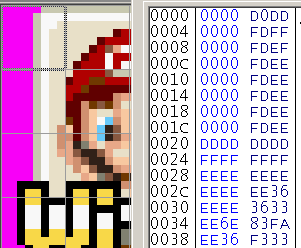
\includegraphics{images/0_home_fast6191_romhackingguide_unrenamed_files_and_original_borders_romhackingendiandemo.png}
\caption{PIC}
\end{figure}

\hypertarget{boolean-logic}{%
\subsection{Boolean logic}\label{boolean-logic}}

Often a more useful set of techniques than basic shifts and the other operations covered already. There are several types although you will probably see patterns soon enough (mainly that the NAND, NOR and XNOR are just the inverse of their counterparts). Boolean logic exists in two big areas ROM hacking and related pursuits might be concerned with; one is programming and the other is electronic logic where they perform identical functions but in some ways are thought of a bit differently.

Here is probably useful to discuss the idea of high and low as it applies to computing and electronics. In the vast majority of cases (especially software and ROM hacking) you should always assume that unless otherwise stated a high value corresponds to 1 and a low value corresponds to 0. This is unlike some other things in this section where you will usually want to seek clarification for things (what method of negative or point numbers you are using for instance). There is however a variation on this called negative edge logic (referring to certain chips that change on the falling edge of a clock pulse) that can be described with the opposite where 0 is high and 1 is low.

Examples will be done in binary.

\textbf{NOT aka inverse} Does what it says and flips every bit.

1001 1110 becomes 0110 0001

\textbf{AND} Here you take two numbers (preferably of equal length but if not the shorter sequence is repeated as appropriate in most cases) and combine the outcome so that only if both inputs are high the result is high

1100 1111 AND 1010 0100 becomes 1000 0100

\textbf{NAND} Much like AND you take two numbers and put them together but rather than if both are high this is if both are low. It is most useful as it is a fundamental logic operation; you can stack NAND operations or indeed NAND gates in such a way that you can make any other Boolean operation.

1100 1111 NAND 1010 0100 becomes 0111 1011

\textbf{OR} Again two numbers but if any one of the inputs it high the result is high.

1100 1111 OR 1010 0100 becomes 1110 1111

\textbf{NOR} Two numbers but only high if both inputs are low

1100 1111 NOR 1010 0100 becomes 0001 0000

\textbf{XOR} Two numbers but only high if only one input is high. Useful as encryption by itself and the basis of many more useful encryption methods. As a quick aside there are serious downsides when it comes to actually being used as encryption, if done properly it is one of the few that can not be broken with enough computing power. Also where the others can easily have multiple inputs in electronics a multiple input XOR is tricky at best.

1100 1111 XOR 1010 0100 becomes 0110 1011

\textbf{XNOR} Two inputs, only high outputs when none or both inputs are the same. Being the inverse of XOR it has similar problems to it.

1100 1111 XNOR 1010 0100 becomes 1001 0100

\textbf{Discussion of Boolean logic.} The most useful in day to day ROM hacking are probably NOT, AND, OR and, purely because of the encryption, XOR.

NOT aka inverse is useful on many occasions for many things especially in graphics (it might not be quite that simple in practice but inverting colours is quite common). Also useful to corrupt data and recover it easily (you just invert it back).

AND is useful to remove certain bits, for instance if you want to remove the highest bit in a byte just AND the result with 0111 1111 and whatever the rest is will stay the same but the highest bit will be 0 regardless.

OR is useful if you want to set a certain bit high, for instance to set the highest bit in a byte high just OR the result with 1000 0000 and the first bit will be set high regardless but the rest will only be high if they were to begin with.

XOR is also used a few times in the internals of the GBA and DS and is used extensively as simple protection at points in cheat devices and things like the GBA e reader.

\textbf{An aside on logical/relational operators} They share the same name and broad function as the boolean logic but here they are used as checks to see if both inputs meet a given condition. In C type languages it runs as follows

AND checks to see if both inputs are non 0 and returns true if it is the case

OR checks to see if just one input is non 0 and returns true if it is the case

NOT merely reverses the output of the other functions.

As far as most of ROM hacking is concerned this will usually be interpreted closer to assembly where compares and branching will be used instead.

Equally a right hand logical shift is different from a conventional right hand shift in that it will retain the most significant bit

1000 1110 right shifted by 1 makes for 1100 0111

\hypertarget{hex-mathematics.}{%
\subsection{Hex Mathematics.}\label{hex-mathematics.}}

Some people can operate in hexadecimal but most of the time the maths resembles long division and long form maths. It is quite useful to know as\ldots{} quickfire round what is 9 + 3 in hex.

The answer is C but courtesy of probably using decimal all your life your immediate thought might well have been 12 which could well mess your entire hack up if you put that into the ROM.

Subtraction works much the same way until you get to negative (signed) numbers in which case you get to figure out what method you are using for it.

Multiplication is easy enough

1D x 09 is 10 x 9 + 0D x 9 or 90 + 75 = 105

Division is a pain and more importantly depends on the programming language function used; many basic methods will chop off the stuff after the ``decimal'' point where others will turn it into a floating number. Floating point might not be that accurate as hex is somewhat less capable of displaying the results of common divisions, not to mention it will be rounded at some point. Such a trick is often used to confuse, and so teach, new programmers and even catches out older ones; finance packages are especially troubled by this for if they miss a couple of rounding points it can result in big amounts of money not going where it needs to go. There are however a few concepts worth noting as they crop up in programming languages and the processors they run on

\textbf{Mod} As mentioned some basic hexadecimal divide functions will leave you with just the whole number part of the result (99 divided by 6 is 16.5 but many divide functions would just give you 16). Mod is then a function that gives you the remainder as a whole number (99 divided by 6 is 16 remainder 3) which you can leave in the hope it will be multiplied back later or feed to another command (many divide functions struggle with large numbers and prefer small ones).

\textbf{Abs(olute)} Potentially confusingly regular maths sometimes also calls this modulus with the shorthand sometimes being ``mod''. Depending upon how far you want to take maths it can get quite complex but the short version is abs value of a number is just the number (always positive) without the sign. It is then quite useful to feed into functions so you can simplify them or the resulting maths.

\hypertarget{patching-and-patch-making}{%
\section{Patching and patch making}\label{patching-and-patch-making}}

ROM hackers change ROM images, copyright lengths being what they are it means such things are copyrighted code. Even edited code still has protections so the differences between the versions are found and made into a patch file, such a thing will also have the very nice bonus of tending to be far smaller and easier to transmit. Patch files then allow someone to take the original ROM, apply the patch to turn it into your changed version and then play it. As with most concepts you can use a computer to help out and, also like most concepts, there many methods by which you can create and apply patches. However unlike most other times where you need to decide between competing formats there is more to it than token differences and vendor lock in. Each type is linked to the best example/implementation at time of writing with a couple more at the end if there are others worth noting.

\begin{itemize}
\tightlist
\item
  \href{https://www.romhacking.net/utilities/13/}{IPS}. The original ROM hacking patching method of choice. It is a truly basic format (the basic form contains a magic stamp/value, a list of patches to apply (which consist of a location, length and payload) and a signal for the end of the file) although there are a few custom versions that are not widely supported. It can not handle location changes which is not a problem for older consoles but with consoles that have filesystems (which is to say most optical media using and post GBA consoles) it is a dealbreaker. It is also limited to files of 16 megabytes in size or less, again this is not a problem on older consoles but even the GBA allowed code up to 32 megabytes to be run.
\item
  \href{http://www.romhacking.net/utilities/519/}{UPS}. Made as a direct successor to IPS it has found some use in older consoles and later GBA patches but came a bit too late and the patching methods below had stolen the spotlight. \href{http://www.romhacking.net/utilities/677/\%20}{Upset}, \href{http://www.romhacking.net/utilities/519/}{Tsukuyomi UPS} and \href{http://www.romhacking.net/utilities/606/}{NUPS} are all good tools for UPS.
\item
  \href{http://www.romhacking.net/utilities/514/}{PPF}. Made originally to patch PS1 games (\textbf{P}laystation \textbf{P}atching \textbf{F}ormat being the longer form) it went through a few revisions and as such some are wary, however it saw some use on the Wii and continues to kick around. Size limits are not really a problem (it is unknown what the upper limit is) and shifts are handled OK. \href{http://filetrip.net/pc-downloads/applications/download-ppf-o-matic-30-f29416.html}{PPF-O-Matic} is a nice GUI patching program and the original \href{http://www.romhacking.net/utilities/353/}{PPF} program should provide a nice multiplatform patching and patch making alternative.
\item
  \href{http://xdelta.org/}{Xdelta}and \href{http://www.daemonology.net/bsdiff/}{BSDiff}. Both general patching formats (indeed they tend to position themselves as rival formats) that got used for the DS and newer consoles (ROM hackers have tended to favour Xdelta where BSDiff saw more use in the form of Scene trainers and patches). Shifts are handled well enough (although they might not be perfect) and sizes are not likely to get to a limit any time soon (although some implementations of BSDiff are rather low). Features some support for original file checking and hashing. The current version of Xdelta was linked but there is an \href{http://www.evanjones.ca/software/xdelta-win32.html}{older version} that was used for a while and there have been some compatibility issues.
\item
  \href{http://www.romhacking.net/utilities/329/}{Ninja}. An earlier candidate to replace IPS and fell out of favour for various reasons. Some patches have been seen to use it and in many ways it works quite well.
\item
  \href{http://www.quickpar.org.uk/}{PAR2}. Not a patching method per se and more of a corruption detection and data recovery format. Changed data is no different to corrupt data as far as it is concerned so can patch programs though it has some trouble with data shifts. Better yet though assuming you have enough redundancy you can be certain your patch will make the original ROM into exactly what you need which is quite useful when there are various corrupt or otherwise modified dumps out in the wild (headers on SNES ROM files for instance).
\item
  Custom. There were some other formats made for various things (Jump Super Stars for instance) and others aimed at more specific things (Fireflower is a patching format aimed at certain graphics hacks for instance) but those will not really be covered here. Some people decided to unpack the ISO/ROM files, patch those individually and build a ROM/ISO afterwards. This made for the smallest patch sizes, usually got around the issue of file relocation, made for some of the best compatibility with various ROM versions and the gave the option to have various options for the patch; a graphics translation might translate graphics that are for the most part decorative, rather than having to make an executive decision you can just make an option at the patch level. The main downside is that it might well be platform specific, require multiple batch files to be made or require runtimes to be installed. Can also help where files are encrypted or compressed and by making a patch you are still technically redistributing code that does not belong to you (encryption and compression looks like differences to a basic compare function).
\end{itemize}

Some people took this custom format concept a step further on the Wii and some other consoles by making a kind of jump loader using a dashboard/menu level console hack to apply a patch to a game's data when it was held in memory. This also had the added bonus of allowing those with the original game and an otherwise unhacked Wii to play the hacked game. Nintendo would do a similar thing to patch a bug in Wii sports resort as the Wii lacks a real patch management feature like the 360 and PS3.

\hypertarget{file-systems-and-operations}{%
\section{File systems and operations}\label{file-systems-and-operations}}

This section will detail the tools and general methods of operation of said tools to pull apart/unpack/extract ROM images. It will probably also be the only section to cover systems other than the GBA and DS in any real detail. The general form of this section is device name, name of method by which hacked code can be run and whether it can be emulated, the names/extensions/types of binaries, any hardware documentation and finally techniques to parse file systems. For additional information or information on systems not covered here then the main sources of hardware information and such like are typically homebrew developers, those wishing to run various flavours of Linux on consoles and emulator authors.

\hypertarget{non-filesystem-devices}{%
\subsection{Non filesystem devices}\label{non-filesystem-devices}}

Method - usually flash carts of various forms which may not exist in an up to date form or be quite expensive if they do exist. Emulation is usually available and very high grade if you want it to be and beyond that everything up to the late 16 bit era and slightly beyond can usually be emulated on newer consoles and handhelds at some level.

As the GBA is a focus of this guide it gets a proper section but in general devices that are older than the DS or do not use optical media will tend not to have a filesystem, this means you get to employ various techniques covered in the GBA section below. They are frequently directly accessible in memory but other than the GBA often have quirks you have to address (mappers in the NES, hirom and lorom in the SNES and Memory Bank Controllers on the original gameboy and GBC). It should be noted that these quirks often afford serious extra capabilities but as well as being hard to deal with they are often extremely difficult to add or remove from a game.

Today other than the GBA you will tend to only encounter a lack of a filesystem when editing the executables for things (although that is not a certainty) and if you get into editing the security/secondary processor/hypervisor programs for the consoles (things like IOS on the Wii and security code for the PS3 Cell coprocessors).

\href{http://www.romhacking.net/?page=documents\&category=12\&platform=\&game=\&author=\&perpage=20\&level=\&title=\&desc=\&docsearch=Go}{romhacking.net} maintains a database of hardware information for older consoles and some newer ones. You may also like \href{http://infrid.com/rcp64/documents.php}{infrid.com for the N64.}

\hypertarget{gba}{%
\subsection{GBA}\label{gba}}

Method - flash cart or emulator.

The GBA is self contained but the executable location (or start thereof and start of the useful stuff) is easily found.

\href{http://problemkaputt.de/gbatek.htm}{GBAtek} and \href{http://www.cs.rit.edu/~tjh8300/CowBite/CowBiteSpec.htm}{CowBite} are usually considered to be the top hardware documents, some more specific documentation for certain hardware areas like the audio setup also exists.

Aside from some homebrew the GBA does not really feature a file system meaning there is not really such a thing as exploding the ROM image into a group of files it is composed of. There is an advanced technique known as tracing though that can find where any data is located in the ROM and a handful of simpler, though sometimes less effective, variations on the theme (BIOS SWI call logging and pointer field searching) that will be covered in the appropriate sections.

Some tools like those seen in Atrius' Golden Sun editors contain searching routines for subfiles, compression can be searched for with various tools, the GBA ``sappy'' audio format such that it is can be detected in some cases and more general tools for games like Pokemon will also contain a listing of the location of various game components (or the things that point at them) as might some other games. Other than flash carts, some undumped ROM images (full length videos) and some of those 30 in 1 carts you find in tourist traps the whole cart is visible in memory at all times and that means the space limit is 32 megabytes.

\hypertarget{ds}{%
\subsection{DS}\label{ds}}

Method - flash cart or emulator. DS and DS lite run GBA code natively if you have a GBA slot cart.

The executable formats for the DS are ARM9, ARM7 and overlay files that usually come with the extension .bin and sometimes SRL.

\href{http://problemkaputt.de/gbatek.htm}{GBAtek} is the main reference document for hardware for the DS.

\textbf{NDStool}

\href{http://filetrip.net/nds-downloads/utilities/download-nintendo-ds-rom-tool-ndstool-1501-f29352.html}{NDStool on filetrip} Command line and very quick and easy but fails to rebuild certain ROM images properly (most still work).

\textbf{Nitroexplorer}

\href{http://filetrip.net/nds-downloads/utilities/download-nitroexplorer-2b-f7301.html}{Nitroexplorer filetrip} Built to make up for shortcomings in NDStool methods. Short of manual editing the go to tool for most.

\textbf{NDSTS}

\href{http://www.no-intro.org/tools.htm}{No-Intro tools page} Able to extract files and insert files of the same size (you can pad them if you want), if it crashes when you have edited it where it worked before with this then it is definitely your fault.

\textbf{Crystaltile2}

\href{http://filetrip.net/nds-downloads/utilities/download-crystaltile2-20100906-f23649.html}{Crystaltile2 filetrip} Able to parse the DS file system as well as extract individual files. Support at this level for compression as well as certain container files as well as support for all sorts of known formats and additional functionality. Click the DS icon on the the icon bar to open the viewer.

\textbf{Tinke}

\href{https://github.com/pleonex/tinke/}{Github link} A tool similar in capability to Crystlatile2 and also supports decompression of files, in ROM and extensive support for other formats.

The DS filesystem is well known and well understood so you have many more options here, indeed it is usually the first feature aspiring DS ROM editing tools gain. DSi compatible games can usually be parsed by standard tools and DSi specific code should now have relevant keys to help things there although it can not really be run. Most games will have archive formats for a handful of files stacked on top but a handful of DS games have been observed to use large single archives for all or most of their files with the files not put into the archive usually being download play components, sound or video.

Most usage will be covered or fairly obvious save for ndstool which has a basic extraction command like

``ndstool -x *.nds -9 arm9.bin -7 arm7.bin -y9 y9.bin -y7 y7.bin -d data -y overlay -t banner .bin -h header.bin''

Replace the -x with -c and the \emph{.nds with a valid name and you can reconstruct a ROM. NDStool is not that useful for end stage hacks but quite useful for quick tests. ``ndstool -l }.nds'' will make a file listing of the files inside a ROM and their locations.

\hypertarget{ds-1}{%
\subsection{3DS}\label{ds-1}}

Various hacks, though things are frequently in a state of flux as it is a modern system that can be updated. Trend is towards custom firmwares, though flash carts also exist. Decryption of whole games is possible, see XORpad and such like, and may have standalone methods before long. Decrypted ROMs may be avaialable online and some files can be obtained from \href{http://gbatemp.net/threads/3ds-cwav-dumper.361437/}{memory dumps}.

Running modified code is well within the scope of the hacks capable of running copied versions of the games.

\href{http://3dbrew.org/wiki/Main_Page}{3dbrew} is the main documentation on the 3ds hardware. A quick overview says it shares a lot of its history with the DS but it is also somewhat closer to a full modern computer architecture (hypervisors/kernels, segmented memory and the like), also features an opengl like implementation of 3d.

\hypertarget{gc-gamecube}{%
\subsection{GC (gamecube)}\label{gc-gamecube}}

Method - mod chip and miniDVD/modded case and regular DVD, SD loader, IDE adapter. Emulators demanding but viable.

boot.dol is the main executable format.

\href{http://hitmen.c02.at/files/yagcd/yagcd/frames.html}{Hitmen YAGCD} is generally considered the better gamecube hardware document.

\href{http://filetrip.net/wii-downloads/other-files/download-gc-tool-120-beta-f818.html}{GC tool}

\href{http://filetrip.net/wii-downloads/other-files/download-gcmutility-05-f606.html}{GCM utility}(mainly multiboot rather than iso handling).

\href{http://filetrip.net/wii-downloads/tools-utilities/latest-gamecube-iso-tool-f28774.html}{Gamecube ISO tool}

\hypertarget{wii}{%
\subsection{Wii}\label{wii}}

Method - Softmod loading from external USB. Modchips and some softmods support gamecube. Emulation demanding but viable.

\href{http://wiibrew.org/wiki/Wii_Hardware}{Wiibrew} houses the main collection of hardware information and information on software internals although there are others that move more into formats and editing of internal software.

.dol is again the main format although ELF appears in homebrew.

Wii games and files come in two original flavours and one used by some iso loading types.

\textbf{Discs} Several tools available but Wii scrubber will be the method of choice here

\href{http://filetrip.net/wii-downloads/other-files/download-wiiscrubber-kit-with-multiloader-140-f4399.html}{Wii scrubber filetrip download}

You might however also consider \href{http://wit.wiimm.de/}{Wiimms ISO Tools} for a nice command line alternative and support for some of the custom formats that became quite popular on the Wii.

\textbf{Virtual console and Wiiware aka WAD files} Not to be confused with doom wad files.

One of the former tools for this was WWpacker but better examples exist in

\href{https://code.google.com/p/libwiisharp/}{libwiisharp example binaries}. Simple tools but can unpack things well.

\href{http://code.google.com/p/showmiiwads/}{showmiiwads}. A GUI tool featuring the ability to unpack wad files and deal with common things done to the files they contain after that.

Many titles also nest things in a format known as u8 (and often combine it yaz0 compression) but both of those tools can extract, decompress and deal with that as well.

\href{http://libwiisharp\%20github\%20page}{https://github.com/BtbN/libwiisharp}

\href{https://github.com/Plombo/showmiiwads}{showmiiwads github page}

\textbf{HDD} Most people do not use whole iso images or the minor tweaks to them any more and will instead use a USB hard drive and maybe a custom format. These come in various formats and layers of support but WBFS is the main method that is often stacked on top of FAT or NTFS filesystems. Wiimms ISO Tools linked above have a measure of support for some of this.

\hypertarget{xbox}{%
\subsection{Xbox}\label{xbox}}

Method - Softmods and hardmods both using minor variations on the idea of internal hard drive or copied DVDs. Emulation not really game playing grade for most things but getting better, the 360 does feature a measure of hacked xbox game support when properly hacked.

The executable format for the 360 is xbe files.

As with most things here there are several options although three go head to head here.

C-Xbox tool

Qwix

Craxtion

\href{http://filetrip.net/oldies-downloads/xbox/iso-hacks-tools/}{Filetrip download (all three)}

\hypertarget{xbox-360}{%
\subsection{Xbox 360}\label{xbox-360}}

Method - no real softmod. DVD mod (does not allow altered games, XBLA or DLC unless combined with one of the following methods), JTAG (required older hardware) and RGH (can be done on most hardware though later updates can be harder to work around) lead to onboard and USB loading. Emulation nowhere near.

\href{http://free60.org/Main_Page}{Free60} features a lot of hardware information.

Xbox 360 games come in two broad flavours with a third method mentioned. The executable format for the 360 is .xex files. These can be extracted further (they are based on the Windows PE/portable executable format used in exe and dll files).

\textbf{Xex} Xextool and xextool GUI are tools that can help here. They can unpack the format, apply various patches both to the files themselves and apply the title update patches.

\href{http://filetrip.net/360-downloads/iso-tools/latest-xextool-f29383.html}{Xextool filetrip download}

\href{http://filetrip.net/360-downloads/iso-tools/latest-xextool-gui-f29384.html}{XextoolGUI filetrip download}

\textbf{Discs} Various programs will extract things, including the ISO checking tool known as ABGX360, but many are unwieldy so e-xiso is the main go to method.

\href{http://alecsis.free.fr/Extract-xiso/}{Extract xiso homepage}

\href{http://filetrip.net/360-downloads/iso-tools/download-e-xisogui-1007-f28976.html}{Filetrip download}

GOD and NXE/hard drive installs have come from discs and have but a few bytes difference between each other. They can be made back into more or less unusable isos with GOD2ISO.

XEX files are the binaries of the 360, there can be several. Patches exist in the form of title updates and can be applies to the XEX files if you really want.

\textbf{XBLA/DLC} PIRS, LIVE and CON. PIRS are signed by MS and can be installed on any 360 without issue. They are mainly sourced from Bethesda game of the year and Borderlands double pack games but there are several more.

LIVE is the format of XBLA and DLC. XBLA demos are full games but a little string is swapped to allow play of the full one (naturally this breaks signing and needs a developer or JTAG/RGH box to run it).

A related set of formats and usually handled by all the same tools. Le Fluffie is one of the main ones.

\href{http://skunkiebutt.com/?page_id=362}{Le Fluffie download page}

\href{http://filetrip.net/360-downloads/other-files/download-le-fluffie-690025-f28975.html}{Filetrip download}

\textbf{USB} Not really a format but one of the main methods of access so it is noted. Later in the life of the 360 Microsoft added support for a custom USB format (in practice it was a reserved section of a USB drive). XTAF.

Supported by several tools but USBXTAF is the main method.

\href{http://filetrip.net/360-downloads/hdd-tools/download-usb-xtaf-xplorer-44-f23780.html}{Filetrip download}

\hypertarget{ps1-and-ps2}{%
\subsection{PS1 and PS2}\label{ps1-and-ps2}}

PS1 - modchip. Emulation available for many years, though can be tricky if you venture into the often superior plugin based emulators.

\href{http://www.geocities.co.jp/Playtown/2004/psx/}{Playtown} has a lot on the PS1 (mainly in Japanese). The romhacking.net link from other systems has a bit of information and \href{http://psx.rules.org/psxrul2.shtml}{psx.rules.org} has some more.

PS2- modchip and some softmod driven network/USB loading possible. Emulation demanding but viable.

\href{http://www.philvaz.com/games/PS2.htm}{philvaz.com} has some good information on the graphics hardware and some internals. \href{http://research.scee.net/files/presentations/agdc2002/PS2forPCprogrammers.pdf}{scee.net (warning PDF link)} has a nice introduction as well.

ISO 9660 was for many the order of the day but later games on the PS1 and many on the PS2 added a dummy setup to that and instead made a new filesystem later on and/or read addresses directly from discs.

For the most part the PS2 was also a standard iso 9660 image that countless tools from the likes of 7zip upwards can open but certain games (most notably Square Enix games for music) used raw LBA reads or a custom file system to read certain parts of the iso images in question. There are a few tools that attempted to detect the signature of the music files and occasionally within the whole image.

LBA reads were also used in anti piracy protection for many of these games.

Both use a version of the executable formats known as ELF as their executables.

\hypertarget{ps3}{%
\subsection{PS3}\label{ps3}}

Method various- softmod (maybe with hardware trigger) leading to USB and hard drive loading. Emulation nowhere close.

Technically the PS3 uses a version of ELF for the executables.

ISO

PUP files (updates)

DLC and PSN content.

\hypertarget{psp}{%
\subsection{PSP}\label{psp}}

Method - softmod loading from memory card (official Memory Stick PRO Duo or microSDHC adapters available) or loading from onboard storage (PSP Go). \href{http://www.ppsspp.org/}{Emulation more possible than before} but undeveloped compared to many other systems.

\href{http://groups.csail.mit.edu/cag/raw/documents/R4400_Uman_book_Ed2.pdf}{PSP MIPS R4000 processor (warning PDF)} is a system developer level breakdown of the PSP processor.

Executable format pbp format (usually called eboot.pbp).

There are a few tools here but UMDGen is the dominant one and there is little reason to use another. It supports extraction, insertion of any length, rebuilding the file locations table and relinking files as well as creation of compressed images.

\href{http://filetrip.net/psp-downloads/tools-utilities/download-umdgen-400-f6743.html}{Filetrip link}

\hypertarget{saturn}{%
\subsection{Saturn}\label{saturn}}

Method- Modchip for the most part. Emulation surprisingly good, though the architecture of the Saturn means emulation is demanding for the relative age of the system.

\href{http://wiki.yabause.org/index.php5?title=Main_Page}{Yabause} (one of the more popular emulators for the Saturn) has a fair bit of hardware information.

A slight variation on the iso format although doable with standard tools.

\href{http://www.rockin-b.de/saturn-patching-enemyzero.html}{Guide involving the manipulation of saturn files}

\hypertarget{dreamcast}{%
\subsection{Dreamcast}\label{dreamcast}}

Method - Simply insert copied disc or use a disc loader known as ``Utopia''. Emulation not bad for some games.

Disc image handling varies. CD burners were a new concept when the DC was released and there were lots of competing formats for optical media, you will then want a standard iso tool to explode it into the component tracks (the good stuff is typically the third track onwards). The tracks function more or less like standard isos, save for the fact that they are offset and most normal iso tools can not handle this as is. Fortunately Iso LBA Fix (isofix) by DeXT exists and will change the LBA to start from zero at which point everything will handle it.

\href{http://dextremes.com/dc/data/index.html}{dextremes.com} has links to some information.

\hypertarget{amiga}{%
\subsection{Amiga}\label{amiga}}

Method - copied discs. Emulation well developed.

ADF images are the most common (ADZ are just zipped versions of ADF) but being sourced from floppy discs they tend to have a filesystem.

\href{http://amigadev.elowar.com/}{amigadev} has a lot of top quality information.

UnADF should allow you to unpack ADF images.

\href{http://lclevy.free.fr/adflib/unadf.html}{Unadf homepage}

\href{http://filetrip.net/pc-downloads/applications/download-unadf-10-f25764.html}{Filetrip link}

\hypertarget{pc-and-related-hardware.}{%
\subsection{PC and related hardware.}\label{pc-and-related-hardware.}}

Method- you control the hardware so disc emulation, cracked executables or method emulation (see Steam emulation)\ldots\ldots{}

Various executable formats depending upon development language and operating system.

A tiny bit more on PC hacking is mentioned later but for simple unpacking.

\textbf{PE}

Windows main format is the PE format which is usually known by the extensions exe and dll. This can be unpacked with many things including the likes of 7zip.

\textbf{ELF}

Used as the basis for a lot of executable formats (including many of the consoles covered elsewhere).

\textbf{Iso}

Broad term for images of optical discs (and sometimes other things) and there are various formats for it (many things will be called iso and burn as one but be unable to be extracted). Can be extracted by many tools including \href{http://www.7-zip.org/}{7zip} and \href{http://www.ezbsystems.com/ultraiso/}{Ultraiso (paid software)}

\textbf{Batch/bash}

Most operating systems provide a command line where commands can be typed and layered on top of this is are the concept of small text scripts that can do fairly extensive things but in practice are just a list of commands with a few extras.

\textbf{Scripts}

(Python, lua, Java, visual basic and many more). Many programming languages operate outside the realms of the standard executable (or have it for a wrapper) and can have their original code, or something close to it, recovered by various means.

\textbf{SD/CF/XD}

A points you may have to copy a SD,CF, XD or some other memory card at the sector by sector level. On these occasions there is a program called DD which is popular on linux and has a \href{http://www.chrysocome.net/dd}{Windows port} too.

\hypertarget{finding-the-object-of-your-interest.}{%
\section{Finding the object of your interest.}\label{finding-the-object-of-your-interest.}}

Games come as ROM images, or if they come from optical media originally then ISO images, but common to both is that they are one large lump of code. The previous section took care of methods to pull apart these initial files but that is only the start of things as you will want to find the relevant file or section that houses the thing you want to look at or change.

There are techniques here ranging from the obvious to the subtle, from the basic to the complex and from the crude to the precise and many will be useless to you without knowing several other things detailed elsewhere in this document. Many ROM hackers starting out will see the more advanced methods of locating data and panic but for the likes of the DS and most other file system sporting devices the main method people use to find the files they want is the file names (most games feature them even if they do not use them directly), file sizes and extensions either directly (English.bmg might well be the text in a DS ROM) or indirectly (sound\_data.sdat will probably be the sound so you can eliminate that chunk from your search for the text for a game which is doubly nice as sound is usually a good portion of space in a ROM) with a quick look at directory names alongside that (sound will probably contain sound, 3d will probably contain 3d and dwc\textbackslash utility.bin is probably download play\footnote{The download play component of a ROM sometimes acts as a cut down version of the main game but pulling it apart and using data gleaned there to attempt to reverse engineer the main ROM is not that useful. It can sometimes net nice artwork maybe provide a few more example files but it is not the first port of call when reverse engineering a DS ROM for most.} ).

Alongside this there are several known extensions and header values for various formats where the first few bytes decode as a known ASCII or hexadecimal string. Many more examples later but for now sdat is an extremely common sound format on the DS and bmg is a fairly common text format. It should be noted that extensions can often give away the presence of compression with common examples being if a file ends with ``.l'' , ``.lz'', ``.\_'' or something along those lines, especially if it has another known extension before it, then it might well be compressed and you can act accordingly.

ROM corruption should also be mentioned here. It gets a bit costly to do if you have to burn discs each time but when emulators and flash carts are available you can corrupt a part of the ROM, run it and when it errors or crashes you get to see what parts do what. The simple method is to use one of the hex operations you learned about earlier but there are dedicated corruption tools. Likewise the technique might need to be refined for certain things as things like graphics can only use a select series of values that the corruption tool might inadvertently use. You can also refine the concept to a point where alteration is probably a better term, for instance when trying to figure out how text is encoded it can be useful to repeat a value or sequence rather than using random garbage.

After this you start heading towards more programming level techniques like relative searching which uses the fact that in Roman character using languages A is followed by B which is followed by C and so should you know the word CAB is in a ROM you can search for a string what has one value followed by a value two less than it and that followed by a value one less than the opening value (although in practice a longer search term is more useful).

Tracing is understood to the be the ultimate method and it is still quite different to simple hex analysis and file names, however it is not that hard to follow along with the basic idea. In tracing you find the thing you want to look at in the memory (if it is on the screen or coming out of the speakers then it is likely in memory), find what put it there, find where that was told to look and so on until you have the location of the file in the ROM or enough data to find it, and possibly also the means by which it is all decoded. Naturally it is quite an involved technique but very accurate and very reliable. When dealing with PC games and to a lesser extent with some emulators you can observe which files are open and loaded when running the game but this is not always available/viable for the consoles. There is the lesser method of watching BIOS calls (BIOS often being used to handle compression can lead you right to the location on the GBA) and you can do things like search for a field of pointers (on the GBA this often means a list of 08 with 3 bytes afterwards as the most common GBA address is of the form 08XXXXXX) which can help.

\hypertarget{abstraction}{%
\section{Abstraction}\label{abstraction}}

Certainly a topic worthy of a document all to itself the main idea here is related to the jargon earlier. Coming at the cost of not being immediately accessible to all (or in this case the computer in question) you build a method by which to interpret something into a format understandable by a target, in this case usually the console in question which translates it to a usable format. Such a move obviously has speed penalties, the bonus however is that you can use a simpler method to store, deal with and hopefully change your chosen item as necessary.

Programming languages are all about this as they all attempt to move away from a user feeding the computer a string of 1s and 0s. A nice example might be to compare the GBA and DS for if you recall the GBA lumps everything into one file where the DS can explode a ROM into a series of other files. Now if you want to add a section of code to the GBA you either change all references to everything after the section you are increasing in size accordingly (a very tedious process that nobody ever does) or add to the end of the ROM (or some other blank space). On the DS your ROM rebuilding tool simply adds the extra to the locations of the subsequent files (and other sizes as necessary) and as the files are not usually tied to each other as whole (obviously files can work together on occasion) nothing is troubled. However when compared to the GBA it does mean the DS will have to do an extra step when it comes to running the ROM to figure out where to point the read command. Much like a unified theory of physics there exists a theoretical but perfect level of abstraction that you could feed an initial value into and have it run accordingly but much like physics you occasionally want to get some actual work done so you cut it off and possibly simplify/restrict things so as to set about getting that something done.

Related to this is that not all the data you see in a ROM will be used in it. For instance any file names contained within subfiles or occasionally even the files themselves might be completely irrelevant, as might be some of the pointers/size values. Generally though it pays to know and understand what each value might mean and account for it as you edit the files unless you can demonstrably prove it does not matter.

This also applies in reverse with some developers choosing to hardcode values somewhere despite not having to or it even being all that good from a programming quality standpoint (as a ROM hacker you might well have to fix several bugs introduced in such a manner); remember that game programmers are people too and are no strangers to the hack something together and knock off for lunch routine.

If a rule of thumb has to be made it would be understanding the level just above the thing you are trying to do will tend to be beneficial and such a logic underpins a lot of the content of this document.

\hypertarget{tools-of-the-trade-continued}{%
\section{Tools of the trade continued}\label{tools-of-the-trade-continued}}

The following simply lists some example tools as there are usually several options for a program to tackle a task, some very basic usage and some screenshots where necessary. In the case of large tools or area specific tools the proper usage will be covered in other parts of this document where there may also be other little tools to help out things. Basic usage of programs to parse relevant filesystems was already covered and will not be covered here. With the exception of the paid hex editors, a couple of audio programs, the debugging/reverse engineering tool known as IDA (a big exception) and some of the translation memory/CAT tools all the programs covered are freeware, often even open source, and everything can be done with the open source/freeware programs.

\hypertarget{hex-editor}{%
\subsection{Hex editor}\label{hex-editor}}

As part of the underlying project this document is part of several hex editors were tested and rated for their usefulness so as to come up with a shortlist. Most ROM hackers will have several at their disposal with each aimed at different tasks. However if you can pick a paid one, get the four freeware suggestions and get a ROM hacking specific one most things can be done with relative ease. In short though a hex editor is a hex editor and everything else is so much extra that could one day make your life slightly easier. The GUI for most of these is extensively customisable but for the most part the images are those of the stock editor with a few menus displayed as appropriate.

The features that make life easier for ROM hackers are

\begin{itemize}
\tightlist
\item
  Bitwise operations
\item
  Boolean logic/operations (sometimes lumped in with bitwise operations)
\item
  Byte flipping
\item
  Search and search all
\item
  Search and replace
\item
  Hex distribution
\item
  Operations on selected areas (some editors will only operate across the whole file)
\item
  Scripting
\item
  Format/structure listing support
\item
  Variable width windows
\item
  Undo/Redo
\item
  Insert
\item
  Hash values including custom options
\item
  String dumps (occasionally you might just want every string in a game even if inserting it back in will be a pain without the surrounding info)
\item
  Custom character encoding support
\item
  Compare files (including size differences/inserted section support)
\end{itemize}

Raw disk editing, program/memory editing, X86 disassembly, base64 decode and similar things are other features that an editor might be sold as having are great but they have been of limited use to ROM hackers in the past, even program/memory editing is usually taken care of by specialist programs as you will see when cheats are discussed.

\textbf{Paid} The freeware editors in many ways provide a more than adequate replacement for the commercial tools but many still like the commercial offerings. The two best ones are quite pricey and are roughly equal in ability.

\textbf{Hex workshop} \href{http://www.hexworkshop.com/}{Hex Workshop homepage}

Probably the most popular paid editor among ROM hackers.

\begin{figure}
\centering
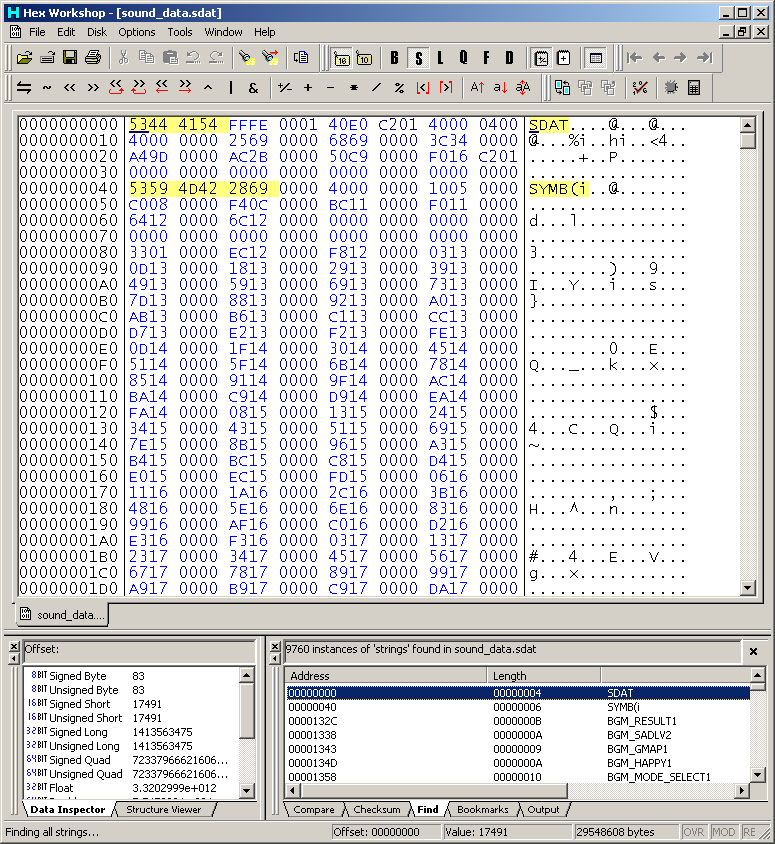
\includegraphics{images/1_home_fast6191_romhackingguide_unrenamed_files___mhackingguidehexeditorsshowcasehexworkshop1.png}
\caption{PIC}
\end{figure}

\textbf{010 editor} \href{http://www.sweetscape.com/010editor/}{010 editor homepage}

Another paid editor on a par with hex workshop

\begin{figure}
\centering
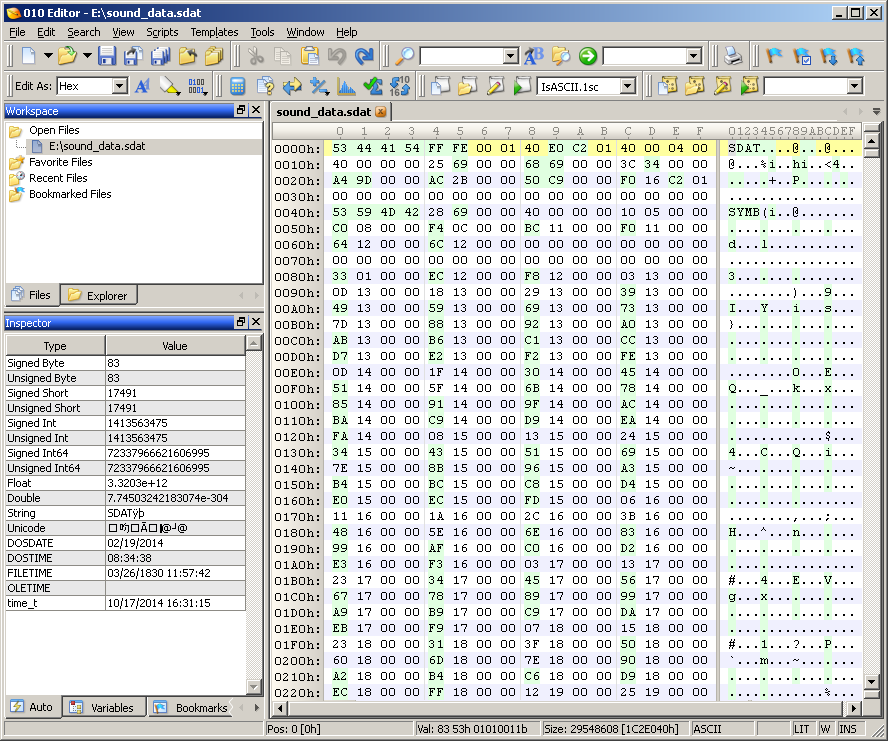
\includegraphics{images/2_home_fast6191_romhackingguide_unrenamed_files___romhackingguidehexeditorsshowcase010editor1.png}
\caption{PIC}
\end{figure}

\textbf{Freeware} The freeware offerings here, unlike some other areas of computing, are not on a par but with a slightly different GUI. However when the suggestions in the freeware category are combined it makes for all the functionality of the commercial offerings.

\textbf{ICY Hexplorer} \href{http://hexplorer.sourceforge.net/}{Sourceforge page}

Almost at the level where you could drop it in as a replacement for the commercial offerings (save for the lack of ability to have multiple files open at once). Needs some setup to get the GUI functioning well but once done it is suitable for use as a day to day editor.

\begin{figure}
\centering
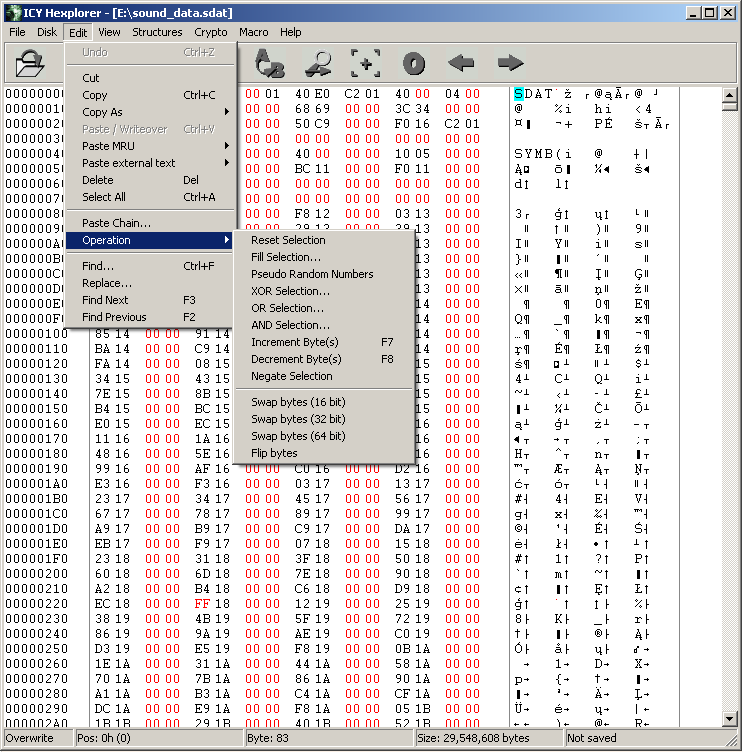
\includegraphics{images/3_home_fast6191_romhackingguide_unrenamed_files___hackingguidehexeditorsshowcaseICYHexplorer1.png}
\caption{PIC}
\end{figure}

\textbf{XVI32} \href{http://www.chmaas.handshake.de/delphi/freeware/xvi32/xvi32.htm}{Homepage}

Still being actively developed and it is mainly here as it features a powerful scripting language which can accomplish most tasks the paid and function heavy freeware editors sport with a bit more after that owing to it being a true scripting language.

\begin{figure}
\centering
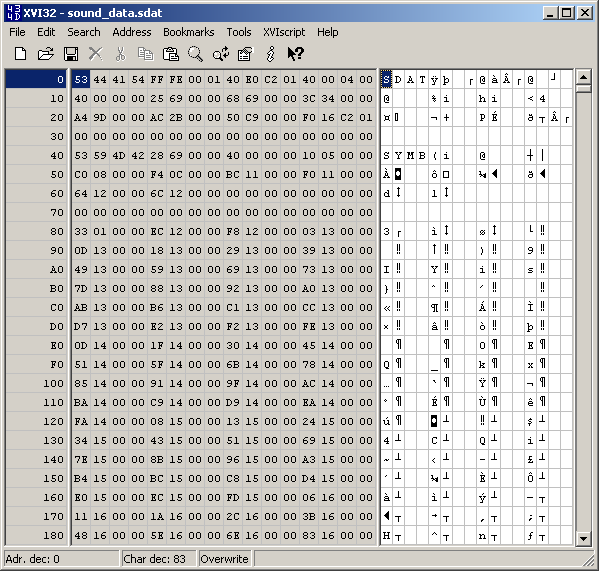
\includegraphics{images/4_home_fast6191_romhackingguide_unrenamed_files___rs_romhackingguidehexeditorsshowcaseXVI32_1.png}
\caption{PIC}
\end{figure}

\textbf{Tiny Hexer} \href{http://filetrip.net/pc-downloads/applications/download-tiny-hexer-1816-f29009.html}{Filetrip download}

A discontinued editor but has some very impressive features the equal of, and sometimes even better than, the commercial offerings.

\begin{figure}
\centering
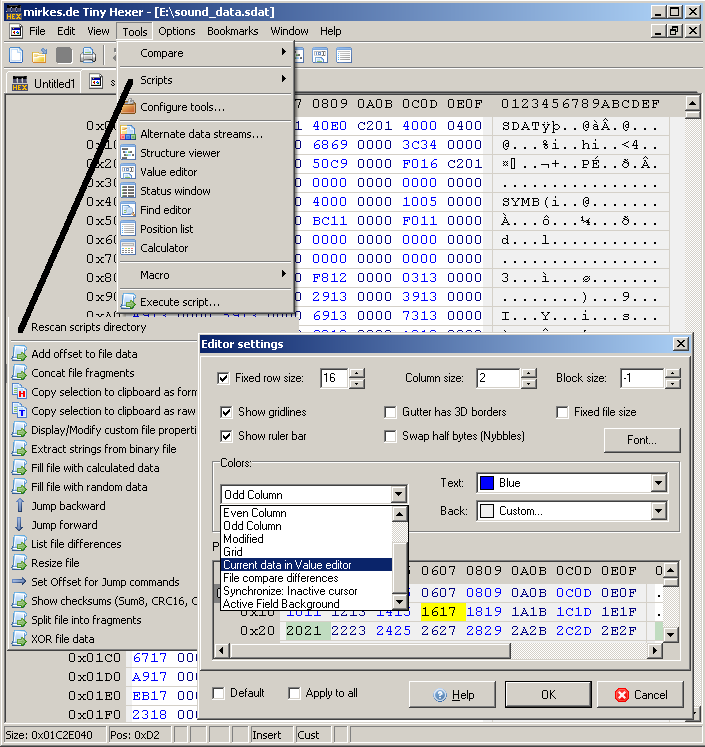
\includegraphics{images/5_home_fast6191_romhackingguide_unrenamed_files___romhackingguidehexeditorsshowcasetinyhexer1.png}
\caption{PIC}
\end{figure}

\textbf{HxD} \href{http://mh-nexus.de/en/hxd/}{Homepage}

\href{http://filetrip.net/pc-downloads/applications/download-hxd-hex-editor-1770-f12907.html}{Filetrip download}

Probably the simplest editor on this list but the go to freeware editor for a lot of people.

\begin{figure}
\centering
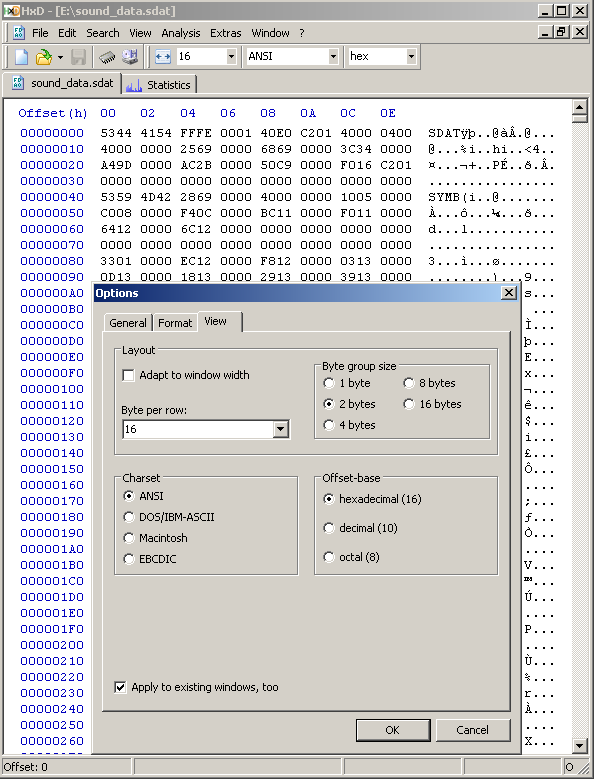
\includegraphics{images/6_home_fast6191_romhackingguide_unrenamed_files___rders_romhackingguidehexeditorsshowcaseHxD1.png}
\caption{PIC}
\end{figure}

\textbf{ROM hacking specific} As wonderful as the editors, commercial or otherwise, above are they lack things like high grade table support (most of the above will support a measure of custom characters but nothing truly custom like that which is seen in hacking) which is fairly essential for text hacking purposes.

\textbf{Crystaltile2} \href{http://filetrip.net/f23649-CrystalTile2-2010-09-06.html}{Filetrip download}

Supports many character sets out of the box and more importantly supports table files.

Lacks boolean manipulations along with the standard hex operations and seemingly fixed to 16 bytes per line.

Has a very good relative search (perhaps not quite as friendly as monkey moore but it works and goes right to up 4 byte/32 bit search as well as many other text grade features covered later)

Has a compression search (mainly type 10 LZ and lesser support for type 11 LZ and huffman).

CRC 16 and 32 are available and can be focused on a selection.

DS filesystem support and header viewing, top flight tile editor/viewer, full ARM9 and ARM7 as seen on the DS disassembler

Support for a fair few SDK and common formats (NARC, SDAT, NFTR, DS 2d formats, some general archive formats)

\begin{figure}
\centering
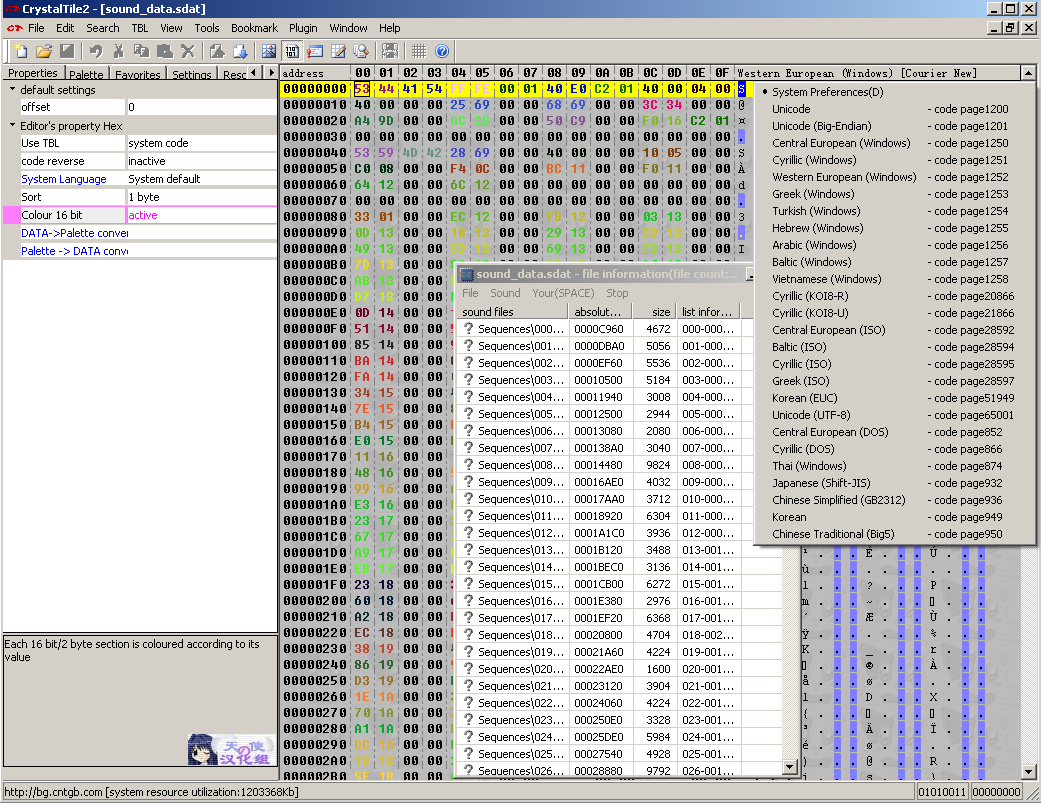
\includegraphics{images/7_home_fast6191_romhackingguide_unrenamed_files___ackingguidehexeditorsshowcasecrystaltile2_1.png}
\caption{PIC}
\end{figure}

\textbf{Windhex32} Not to be confused with the popular disk forensics grade hex editor ``\href{https://www.x-ways.net/winhex/}{winhex}'' which is not in the paid list owing to a lack of bitwise features and similar things (it is very good at disk forensics though).

\href{http://www.romhacking.net/utilities/291/}{Romhacking.net page}

Great table and text support (including multitable support you can switch between), some SNES specific memory mappings and SNES/NES tile editor. Mainly just a very nice text capable hex editor with table support and some tools to complement that. It lacks undo support and some GUI choices are a bit odd which prevents it from being a drop in replacement for HxD.

\begin{figure}
\centering
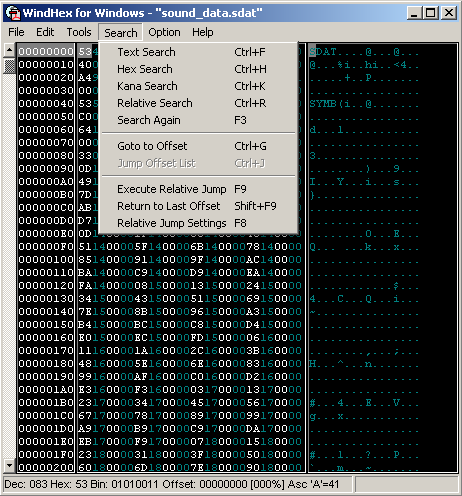
\includegraphics{images/8_home_fast6191_romhackingguide_unrenamed_files___omhackingguidehexeditorsshowcasewindhex32_1.png}
\caption{PIC}
\end{figure}

\begin{figure}
\centering
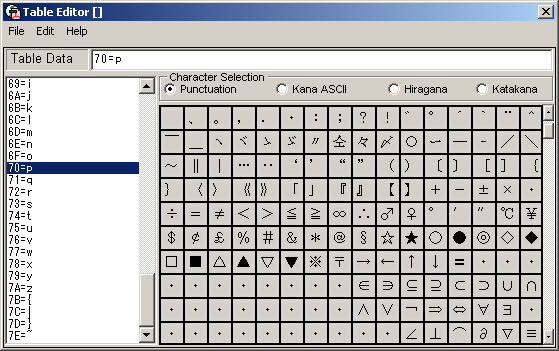
\includegraphics{images/9_home_fast6191_romhackingguide_unrenamed_files___omhackingguidehexeditorsshowcasewindhex32_2.png}
\caption{PIC}
\end{figure}

\textbf{Goldfinger} \href{http://www.romhacking.net/utilities/204/}{Romhacking.net page} Not to be confused with the GBA assembler Goldroad, the common translation of the Chinese term for cheats or the the common translation of the Chinese term for cart pins.

Support for 9 tables at once, it does not come with ASCII readout as standard so you will have to find/make one. It does feature some table editing abilities.

Although not quite suited to full text display it is unlike most other editors in that it is not necessarily bound by the end of the line. This makes it a nice choice for text editing without having to make a custom tool or dump the text and attempt to get something done in a more conventional text editor.

\begin{figure}
\centering
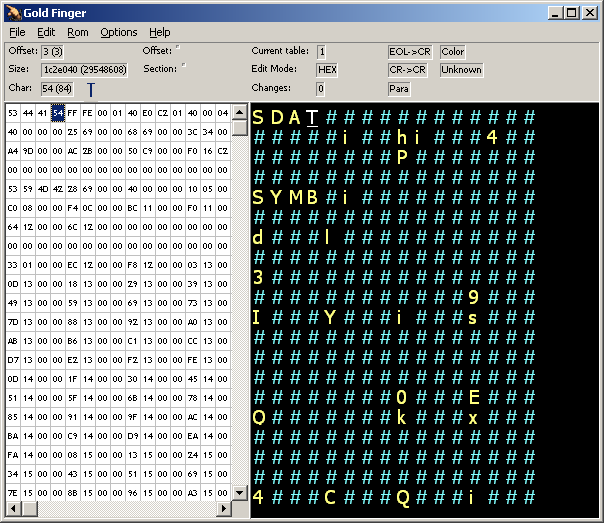
\includegraphics{images/10_home_fast6191_romhackingguide_unrenamed_file___omhackingguidehexeditorsshowcasegoldfinger1.png}
\caption{PIC}
\end{figure}

\textbf{Translhextion} \href{http://www.romhacking.net/utilities/219/\%20}{Romhacking.net page}

New fork/version \href{http://www.romhacking.net/forum/topic,14373.0.html}{Romhacking.net forum thread}

For many the standard ROM hacking hex editor for a long time now (although crystaltile2 is edging it out a bit).

Adjustment of hex window size possible via editor but not grouping.

Jump including relative jump support available and can manipulate bits

Can search using tables and relative search support is available.

No undo support but a nice read only option by pressing tab.

\begin{figure}
\centering
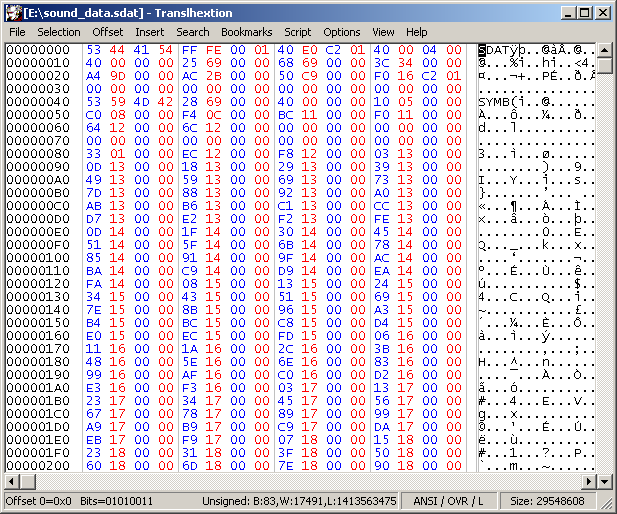
\includegraphics{images/11_home_fast6191_romhackingguide_unrenamed_file___ackingguidehexeditorsshowcasetranslhextion1.png}
\caption{PIC}
\end{figure}

\hypertarget{tile-editor}{%
\subsection{Tile editor}\label{tile-editor}}

Although you can edit anything with a hex editor it gets very complex to do anything other than the most basic editing using one and the first thing to move to a higher level tool is 2d graphics which get a tile editor. There are several available although only a handful will be focused on here. Various homebrew development kits have some nice programs as well aimed at conversion from common formats to the somewhat odd formats used by the handhelds and other consoles.

\textbf{Crystaltile2} \href{http://filetrip.net/f23649-CrystalTile2-2010-09-06.html}{Filetrip download}

Features one of the best tile editors out there (support even for the odd custom hardware display formats and a tile editor capable of being set to arbitrary widths) and has support for various DS image formats on top of the DS file system itself. Exporting and importing images is also possible.

\begin{figure}
\centering
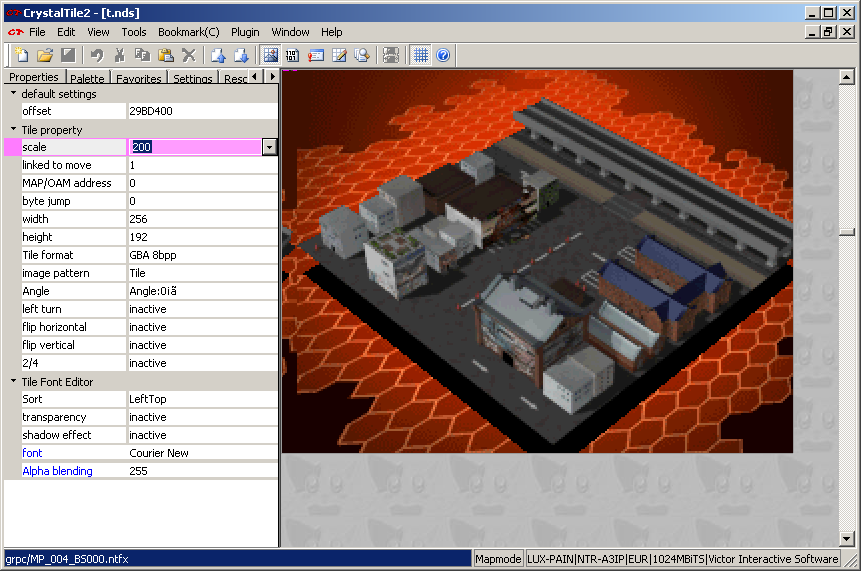
\includegraphics{images/12_home_fast6191_romhackingguide_unrenamed_file___kingguidetileeeditorsshowcasecrystaltile2_1.png}
\caption{PIC}
\end{figure}

\textbf{TileEd2002} \href{http://home.arcor.de/minako.aino/TilEd2002/}{Homepage}

\href{http://filetrip.net/gba-downloads/tools-utilities/download-tiled2002-064b-f7846.html}{Filetrip download}

A GBA vintage editor but as the GBA and DS hardware are largely the same it can get far. It can do basic sized tiles in the two most common hardware formats and has a nice palette fiddling option (one colour at a time if you want), something which some of the others lack and thus is useful when trying to figure out what amount of padding a palette format uses. Lacks support for highly custom tile sizes (it will crash if you try on GBA format imagery) although it does support loading of savestates to get palettes directly from those. Note also the use of imagery to display text as opposed to a text rendering engine; such a thing is very common in smaller puzzle games where there is not much need for actual text, for use in stylised text and in menus in general.

\begin{figure}
\centering
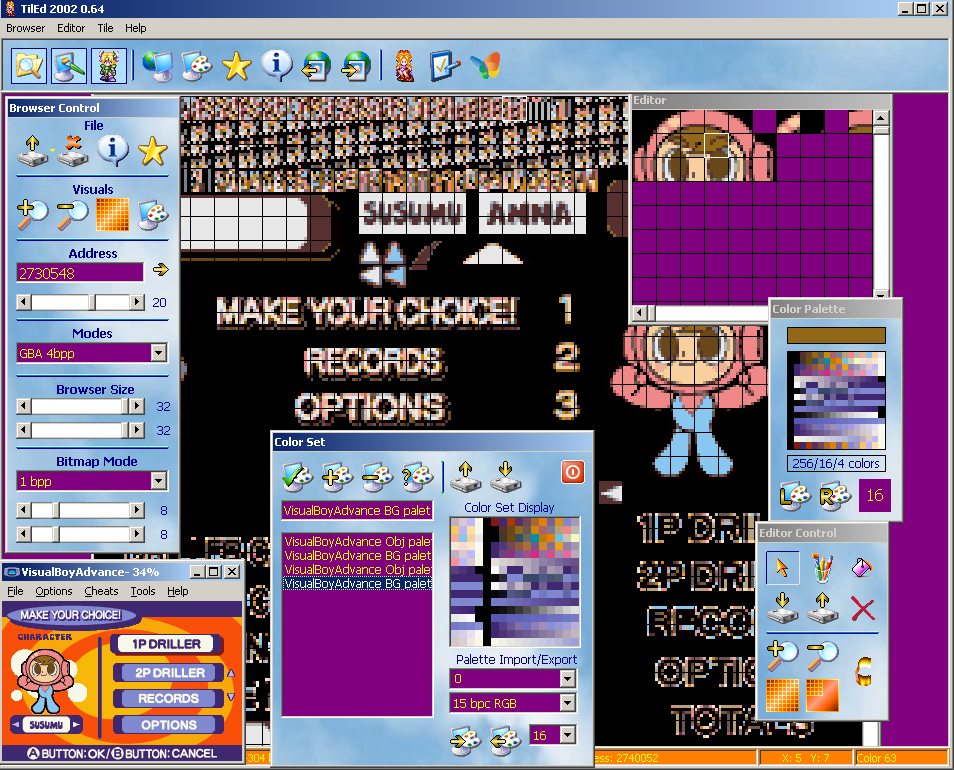
\includegraphics{images/13_home_fast6191_romhackingguide_unrenamed_file___hackingguidetileeeditorsshowcasetiled2002_1.png}
\caption{PIC}
\end{figure}

Also the palette as held in the GBA.

\begin{figure}
\centering
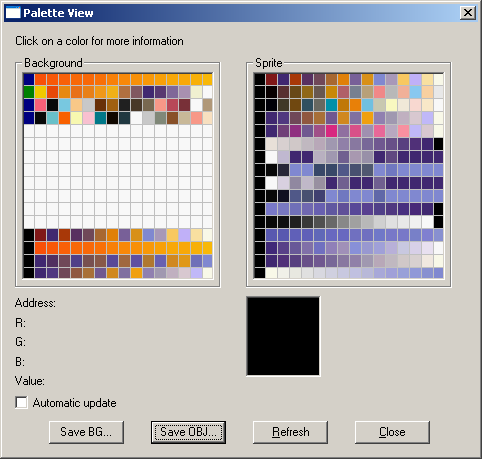
\includegraphics{images/14_home_fast6191_romhackingguide_unrenamed_file___detileeeditorsshowcasetiled2002VBApalette_1.png}
\caption{PIC}
\end{figure}

\textbf{TileGGD} \href{https://github.com/barubary/tiledggd}{Github page}

\href{http://www.romhacking.net/utilities/646/}{Romhacking.net download}

Although the above two should do for most editing purposes this program has hugely customisable support meaning most conceivable hardware formats should be covered (from 1 to 32bpp with big and little endian support) and in some ways has a slightly nicer user interface than crystaltile2. Unlike the other two there is no editing capability built into the program but there is export and the information can be used to direct an editor of another program.

\begin{figure}
\centering
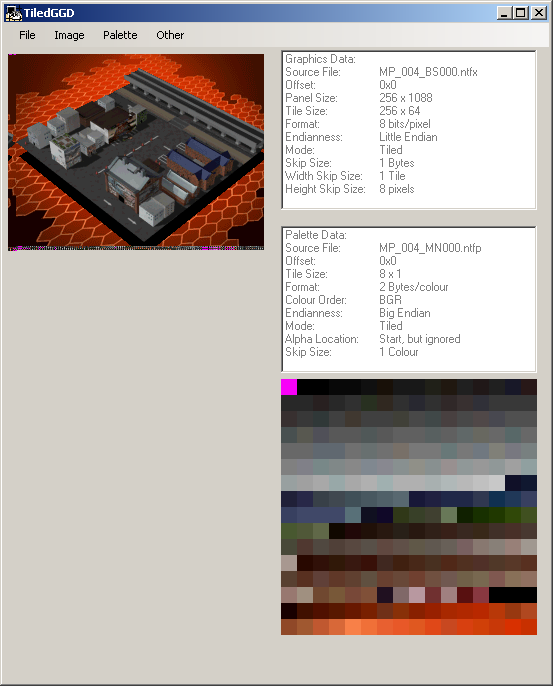
\includegraphics{images/15_home_fast6191_romhackingguide_unrenamed_file___romhackingguidetileeeditorsshowcasetileggd1.png}
\caption{PIC}
\end{figure}

\hypertarget{spreadsheet-and-command-line}{%
\subsection{Spreadsheet and command line}\label{spreadsheet-and-command-line}}

The following is a few basic tools that can be used to help out when ROM hacking when existing tools fall short and before/instead of jumping to programming a game/format specific tool.

\textbf{Libreoffice usage} \href{http://www.libreoffice.org/}{Office suite homepage}

\href{http://help.libreoffice.org/Calc/Welcome_to_the_Calc_Help}{Calc usage/help page}

Calc is the libreoffice spreadsheet program and it supports hexadecimal after a fashion. It is certainly no substitute for a fully realised programming language but it has proven quite valuable when making quick and dirty scripts or reverse engineering formats.

There are seven main operations that get done beyond the basic addition, subtraction and multiplication.

\textbf{Pasting} At least one of your hex editors should have a text export option that when you have set the appropriate amount of columns can export a text list of the hexadecimal (effectively making an array) and equally a search option should be able to export the results. Either way you will need to paste this into the spreadsheet which for the most part is fairly intuitive and automated but you will occasionally have to import as a fixed width or as a delimited set of text (usually a space or tab doing the delimiting). Merging cells (say for a 32 bit value spread across 2 columns where you do not want to change your editor's behaviour) can be done but the quick and easy way is to paste the columns into a text editor and search and replace for the delimiting value.

If you must though you are better off abusing a maths function and multiplying by the appropriate hexadecimal value (65025 and 255 to shift the hex equivalent by 2 and 1 bytes respectively) and the reverse using mod, floor and other functions.

Bitwise, boolean and flipping operations are best done in a hex editor and given the option you will also want to import as text (all the functions will still work) as numbers have a habit of being parsed to something.

\textbf{Fill} A basic command/option but not one everybody knows about. In the bottom right corner of a given cell when selected there will be a small square which you can click and hold before dragging down or up (or across) and the cells have the contents replicated in the cells covered by the drag range. If you have a pattern it will tend to be continued and if you have a formula that will tend to be continued but the cell contents aligned to the same thing (if the original was c4 - c3 the next will likely be c5-c4), it is not foolproof and some of the more advanced things you want want to do can be tricky to pull off but it has worked far more often than it has not.

\textbf{Dec2hex and hex2dec} Although calc does support hexadecimal and you can combine items into one function it is usually easier to have the initial hexadecimal values, the decimal equivalents and the conversion back again.

In calc the commands are dec2hex to convert from decimal to hexadecimal and hex2dec to do the opposite.

\textbf{Differences} Granted this is more of a technique than an actual function but it is the most used concept that actually changes/generate data. If you have a field of pointers (covered later but the general idea is a value that contains the location of another value) and the results of a search for something that indicates the start of a value you might need them to line up but it might not be readily apparent. Most of the time with pointers values change between them (if the data is a fixed distance apart there is no need to incur the time penalty for looking up the pointer and maybe doing some operations upon it) and this can give things away. To do this simply take the next pointer value and subtract the current one. The result will be the difference and if you do it for an unknown pointer set you can quite easily match things up and determine if they are ``out'' by a given amount. You can do a similar thing in reverse to generate new file lengths to save calculating and changing an entire pointer table by hand but by this point it is probably better to build a proper program.

Rounding function As mentioned data tends to like to be found at 8,16 or 32 bits or some other interval (several file formats on the DS have been observed to align to an address that is a multiple of 100h). CEILING is the main function here although remember it takes decimal input for the number to round to. MROUND can also be used in a pinch but remember it can also round down which would be bad so best to add an amount if you are going to use that.

\textbf{Sort function} Not quite so useful in ROM hacking as it is in day to day use is the ability to sort by a value (either letter order or number order)

\textbf{True/false queries and parsed data} Humans are not so good at recognising and interpreting numbers at pace but nice coloured squares are a different matter and quite possible in various spreadsheets. Still if you must use numbers 1 and 0 are easier to account for than lengthy values and spreadsheets can then help with this. The basic method uses the IF command and is typically formed ``IF(some value/cell, equals/is less than/is greater than, then FALSE/TRUE)'' but deleting as appropriate.

\textbf{Filecutter} \href{http://crackerscrap.com/}{crackerscrap.com (click on downloads)}

Usage: filecutter file.in length file.out \textless-s start\textgreater{}

As windows lacks the ability to slice up files from the command line you have this program. Once you have your list of addresses you can use this to generate a batch file with the addresses as the arguments and although it will be specific to that incarnation of the file (not such a problem if you just need everybody to slice up the file as it comes from the ROM) you have just built an archive unpacker. If you need to couple it with a decompression tool you can do that as well in just a few extra steps back in the batch file stage.

Input is in decimal by default but hex can be used if you stick 0x in front of the relevant numbers.

\textbf{Getmyhex} \href{http://www.romhacking.net/utilities/504/}{Romhacking.net download}

\href{http://filetrip.net/pc-downloads/applications/download-getmyhex-1500-f29200.html}{Filetrip download}

A simple tool to get the hexadecimal readout of various short sections of text.

\textbf{Radare(2)} \href{http://radare.org/y/}{Project homepage}

Now taking the place of the Romulan program featured in earlier editions. It is a scripting language but not quite, it is aimed at reverse engineering purposes though the focus is more on the PC and related platforms.

\hypertarget{compression}{%
\subsection{Compression}\label{compression}}

Compression was once the bane of ROM hackers but it got a lot easier to handle on the DS and is not so bad for the GBA either. At this point it might even have reduced to making for a simple extra step using a known tool when extracting something from a ROM or putting it back in but not much else.

\textbf{DSdecmp} \href{https://github.com/barubary/dsdecmp}{Github page}

Supports compression and decompression of LZSS formats seen on the GBA and DS (type 10, 11, 40 and binary/BLZ), RLE and Huffman.

\textbf{Cue's GBA DS compressors} \href{http://gbatemp.net/topic/313278-nintendo-dsgba-compressors/}{GBAtemp thread}

\href{http://filetrip.net/nds-downloads/utilities/download-cues-gba-ds-compressors-10-f29010.html}{Filetrip download}

Also supports compression and decompression of LZSS formats seen on the GBA and DS (type 10, 11, 40 and binary/BLZ), RLE and Huffman as well as LZE (used in Luminous arc titles).

\textbf{Crystaltile2} \href{http://filetrip.net/f23649-CrystalTile2-2010-09-06.html}{Filetrip download}

Has a measure of compression support built into the file manager (type 10, type 11, binary decompression support some RLE and maybe Huffman) and support for some compression searching options. Somewhat buggy but you can learn them and play to them well enough.

\textbf{GBA specific} BIOS and to a lesser extent general LZ compression can be searched for as it makes fairly distinctive changes to the hex. There are also a few tools geared towards being able to deal with GBA ROM images directly and work around issues stemming from a lack of a filesystem.

\textbf{GBA Multi DeCompressor} \href{http://www.romhacking.net/utilities/431/}{romhacking.net download}

Can be directed and fed VBA SWI logs (SWI being the name for the BIOS calls and as mentioned the BIOS in the GBA and DS feature decompression functions).

\textbf{NLZ-GBA Advance} \href{http://www.romhacking.net/utilities/529/}{romhacking.net download}

Ostensibly a graphics editor but one with compression support and compression searching.

\textbf{unLZ-GBA} \href{http://www.romhacking.net/utilities/362/}{romhacking.net download}

A slightly older tool but one of the few ones capable of compression searching.

\textbf{Lz77restructor2} \href{http://filetrip.net/gba-downloads/tools-utilities/latest-lz77restructor2-f29641.html}{Filetrip download}

A newer tool with abilities in graphics and text extraction and insertion/edition on top of the ability to search for compression and restrict those searches.

\textbf{GBADecmp} \href{http://www.romhacking.net/utilities/433/}{romhacking.net download}

A simple tool to decompress and recompress data from/to a known location.

\textbf{Crystaltile2} \href{http://filetrip.net/f23649-CrystalTile2-2010-09-06.html}{Filetrip link}

Supports type 10 LZ which is the same as the GBA BIOS LZ compression. Also supports compression searching.

\textbf{GBACrusher} \href{http://filetrip.net/gba-downloads/tools-utilities/download-gba-crusher-010-f28823.html}{Filetrip link}

A tool to compress files using GBA BIOS compatible compression methods like the 8 and 4 bit Huffman compressions, Differential, Run length encoding, LZ (type 10) for VRAM and for WRAM. Command line version included.

\begin{figure}
\centering
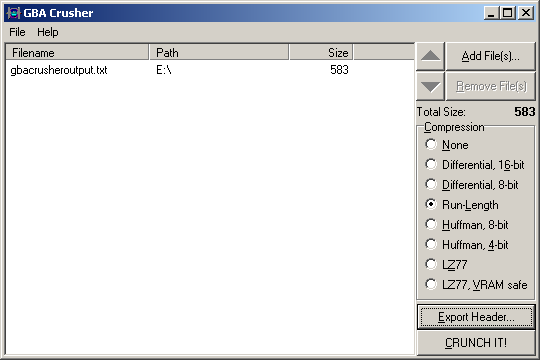
\includegraphics{images/16_home_fast6191_romhackingguide_unrenamed_file___hackingguidecompressionshowcasegbacrusher_1.png}
\caption{PIC}
\end{figure}

\hypertarget{music}{%
\subsection{Music}\label{music}}

Format and console specific tools will be covered in the relevant sections. However a few high level tools are useful to have.

\textbf{Wave editing - Audacity} \href{http://audacity.sourceforge.net/}{Audacity Sourceforge page}

Imports most wave, PCM and ADPCM variations and features editing, some mixing ability and filters.

\textbf{Tracker format - Open MPT} \href{http://openmpt.org/}{Open MPT homepage}

A fairly advanced program with support for playing, editing and exporting various tracker formats. Should have a measure of DLS support although it can be problematic. Formerly known as ModPlug Tracker which is what some tutorials written before the rename will refer to it as.

\textbf{Midi specific - Anvil Studio} \href{http://www.anvilstudio.com/}{Anvil studio homepage}

A freeware program that several of those editing audio for the GBA like to use.

\textbf{General editing - Awave studio} \href{http://www.fmjsoft.com/awframe.html}{Awave studio homepage}

A largely paid piece of software that can help convert files and deal with less than perfect implementations of some audio formats various game specific tools might output. Midi and DLS support is available.

\hypertarget{asmassembly}{%
\subsection{ASM/Assembly}\label{asmassembly}}

Usage is often as extensive as assembly itself but some tools none the less

\textbf{Emulators (debugging/hacking grade)} The following is a list of emulators that possess debug functions of a grade that is useful to ROM hacking without going to abstract methods of debugging.

\textbf{DS} there are a handful of emulators available but only three have any real support for commercial ROM images and debugging.

\textbf{Desmume}

\href{http://desmume.org/download/}{Desmume download page}

The developer and regular versions feature memory viewers, disassemblers, VRAM, OAM and other such viewers. Also features support for GDB and \href{http://wiki.desmume.org/index.php?title=Faq\#What_is_this_Lua_stuff_I_see.3F}{LUA type} debugging as seen in high grade hacking focused emulators like \href{http://www.fceux.com/web/help/LuaScripting.html}{FCEUX}. Its cheat making options are fairly well developed nowadays as well.

\textbf{no\$gba}

\href{http://problemkaputt.de/gba-dev.htm}{no\$gba developer version page}

The gaming version of no\$gba features very few debugging features (although there are some memory editors that interface with it) but there is a debugging version, which is now free to download, available with extensive debugging abilities. Note that ROM images may well need to have their secure area encrypted to run but \href{http://www.no-intro.org/tools.htm}{eNDryptS Advanced} should be able to handle that.

\textbf{iDeaS}

\href{http://ciacin.site90.com/ideas.php}{iDeaS homepage}

Though slightly less developed than Desmume on the commercial ROM front it does however support something closer to breakpoints as seen in no\(gba and the GBA emulators as standard. Function logs and run to selection command are more prominent in the debugging section though and it is not quite a full replacement for no\)gba.

\textbf{GBA} The GBA has a somewhat larger and more featured collection of debugging grade emulators.

\textbf{VBA-SDL-h}

\href{http://labmaster.bios.net.nz/vba-sdl-h/}{VBA-SDL-h Homepage}

\href{http://sharesource.org/project/vbasdlh/}{VBA-SDL-h sharesource page}

\href{http://filetrip.net/gba-downloads/emulators/download-vba-sdl-h-r070904a-f28914.html}{Filetrip download}

Version of the popular GBA emulator reworked to add debugging support like the ability to set breakpoints.

\textbf{VBA-h}

\href{http://filetrip.net/gba-downloads/emulators/download-vba-h-172-f28913.html}{Filetrip download}

VBA-sdl-h above is geared towards assembly hacking and lacks much in the way of a GUI where VBA-h is geared towards memory viewing and cheat making.

\textbf{no\$gba}

\href{http://problemkaputt.de/gba-dev.htm}{no\$gba developer version page}

Along with the DS the GBA is well supported in the debugging editions of no\$gba.

\textbf{BoycottAdvance}

\href{http://filetrip.net/gba-downloads/emulators/download-boycottadvance-028-windows-f28912.html}{Filetrip download}

Some prefer this to VBA-SDL-h and it certainly is a bit more GUI happy. It can take a bit more to get some ROM images working and some of the features are not as extensive but it does have breakpoints which counts for a lot.

\begin{figure}
\centering
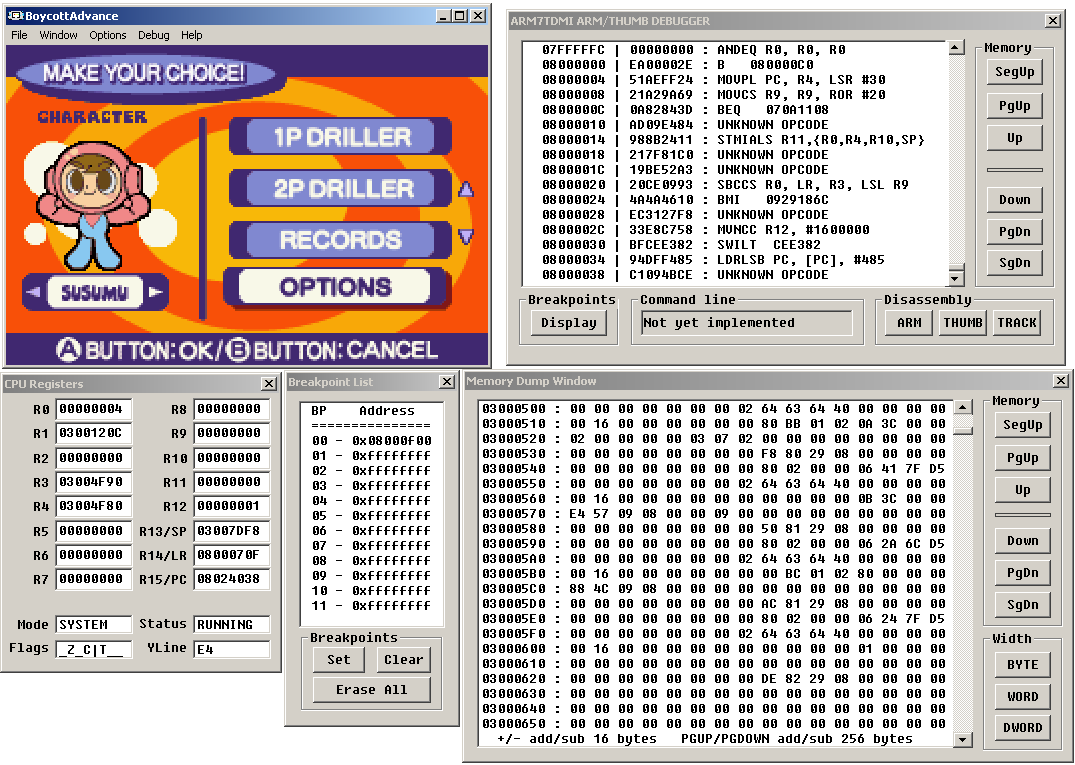
\includegraphics{images/17_home_fast6191_romhackingguide_unrenamed_file___ackingguideemulatorshowcaseboycottadvance_1.png}
\caption{PIC}
\end{figure}

\textbf{Disassemblers} Disassemblers are tools that can be directed to turn machine code and related information back into assembly code. They are pretty dumb for the most part and their output will tend not even to be able to be reassembled without some modification by a human, however take the time to set one up properly for the task you want and they are invaluable.

\textbf{GBA and DS} Emulators will usually provide some disassembly and as they know what mode the processor is running in at the time and have various viewers for memory (video, normal or otherwise) they can be even more useful but standalone disassembly tools do exist. Note that the DS does feature a custom, albeit widely supported, compression format that its binaries can and do use.

\begin{itemize}
\tightlist
\item
  Crystaltile2\href{http://filetrip.net/f23649-CrystalTile2-2010-09-06.html}{Filetrip download}. Has a basic disassembler for ARM9 and ARM7 built into the program and the ability to interface with other programs.
\item
  NDSDIS2 \href{http://hp.vector.co.jp/authors/VA018359/nds/ndshack.html}{NDSDSI2 homepage} \href{http://filetrip.net/nds-downloads/utilities/download-ndsdis2-223-f28977.html}{Filetrip download}. A basic standalone disassembler aimed at the DS.
\item
  arm-eabi-objdump \href{http://devkitpro.org/}{Part of devkitpro/GNU toolchains}. Not so useful on ROM images/for single files only and does not support compression but should work well if you can get it something it can sink its teeth into. If dealing with newer systems then looking at these sorts of toolchains will get you something.
\item
  IDA \href{http://www.hex-rays.com/products/ida/overview.shtml}{IDA homepage} Paid software, the freeware edition is quite locked down though (basically X86 or nothing). This is the go to general purpose disassembler/debugging tool and one all new disassemblers and debugging plugins/tools for various platforms tend to be written for.
\end{itemize}

\textbf{Assemblers} The processors in the GBA and DS are quite similar so you can usually go from one to the other. Developer no\$gba and crystaltile2 feature single instruction editing and IDA has some abilities in this arena too. Also tending to be 16 or 32 bits in length you can often edit instructions by hand. This will focus more on hacker grade assemblers, mainly as programming grade assemblers have great features like the ability to create variables/human readable references and similar things by default where hacker grade ones tend to require more raw input (although armips does have a lot of niceties here).

The GBA ARM7 and DS ARM9 are very similar and the added instructions for the DS ARM9 (all of three which are not all that commonly used) you can live dangerously and switch between them. Since the earlier versions of this document ARM have risen up even further in the world (they basically own all of mobile phones and tablets) so if you are using newer tools, or ones not suggested here, then make sure you are using the right modes.

Again assembly will be covered later (including some links to the official specifications) but in the meantime \href{http://imrannazar.com/ARM-Opcode-Map}{imrannazar.com ARM Opcode Map} has a full listing in a more readable form.

\textbf{armips}

\href{http://www.romhacking.net/utilities/635/}{romhacking.net download}

\href{http://aerie.wingdreams.net/?page_id=6}{program homepage}

A relative newcomer in the ROM hacking assembler world (the first release was back in September 2009). Geared towards GBA and DS ROM hacking (also MIPS R3000 for the PS1) it has the option to use macros, labels (global and local), can load tables so as to be able to load custom strings and something closer to C/C++ family maths than the average assembler. Owing to the way it works it has pretty good support for overlays as well.

\textbf{ARMeabitoolchain}

ARMeabi deals with the underlying assembler for the GNU development toolchains (although for the GBA/DS specific stuff you will want to be looking at \href{http://devkitpro.org/}{devkitpro}).

As part of an earlier hacking project a kit was made to assemble small file fragments into things that could be dropped into the ROM. Two main methods aimed at hacking here

\textbf{cracker's ARM ASM kit}

\href{http://crackerscrap.com/}{crackerscrap.com (click on projects)}

\href{http://gbatemp.net/up/cr-dstmt.zip}{gbatemp download (older version)}

\textbf{Garmy}

\href{http://www.romhacking.net/utilities/456/}{romhacking.net download}

For the GBA you may also like \href{http://forums.nesdev.com/viewtopic.php?f=5\&t=10176\&start=0\#p113532}{this script from Dwedit.}

\textbf{goldroad}

\href{http://www.romhacking.net/utilities/343/}{romhacking.net download}

For quite a while the main assembler available for the GBA as far as ROM hacking was concerned. It is not the cleanest tool out there but can get things done and for some armips replaced it but the above tools are now the preferred method.

\textbf{armish}

\href{http://common-lisp.net/project/armish/}{Project homepage}

Written in lisp and aimed more at homebrew programming it is another assembler for the ARM processor family.

\textbf{arm sdt}

More of a programming assembler and features some very nice functions to help with program development. Many of the GBA homebrew emulators, and some versions of moonshell on the DS, were coded using this in preference to the GNU toolchains, something which made maintenance, forking and third party contributions more difficult in some cases.

\textbf{FASMARM}

An ARM plugin for the X86 and x86-64 assembler \href{http://flatassembler.net/}{FASM}. You can find FASMARM \href{http://arm.flatassembler.net/}{here}.

\hypertarget{basic-file-format-concepts}{%
\section{Basic file format concepts}\label{basic-file-format-concepts}}

Much of the rest of this guide revolves around being able to pull part file formats and it will be covered and related back a bit to the underlying hardware and the concepts the area is based on but there are things to look for when pulling apart a file.

\textbf{Identifiers}

also known as magic stamps these are small lengths of usually ASCII text or hexadecimal that are ``unique'' to the start of a given file format, section thereof or command.

\textbf{Lengths}

most times the lengths of a file or the files contained within an archive format are very important to have. It need not be present if you can calculate the lengths otherwise.

\textbf{Pointers}

as well as lengths the locations of the files are useful to have as are the sub sections of a complex file format and these will tend to have values that state the location of them (point if you will).

\textbf{Header}

the start (or sometimes end) of a file that often houses information on the rest of the file.

It gets a lot more complex, area specific and there are various methods and pitfalls some of which have already been mentioned (things like word alignment) but if you can find one or more of the above and document those you will usually be well on your way to reverse engineering a file format.

Also for an example on why your hex editor will want to be able to change the size of the window (preferably when maximised and with a simple click and drag of the mouse)

Just having opened the file and then after quick resize and a tiny delete

\begin{figure}
\centering
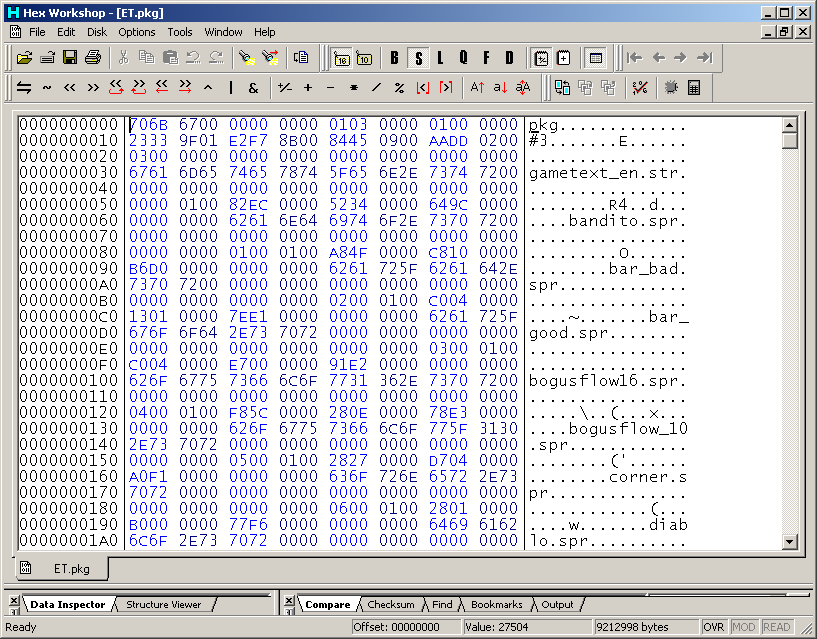
\includegraphics{images/18_home_fast6191_romhackingguide_unrenamed_file___borders_romhackingguidebasicfileformatshex1.png}
\caption{PIC}
\end{figure}

\begin{figure}
\centering
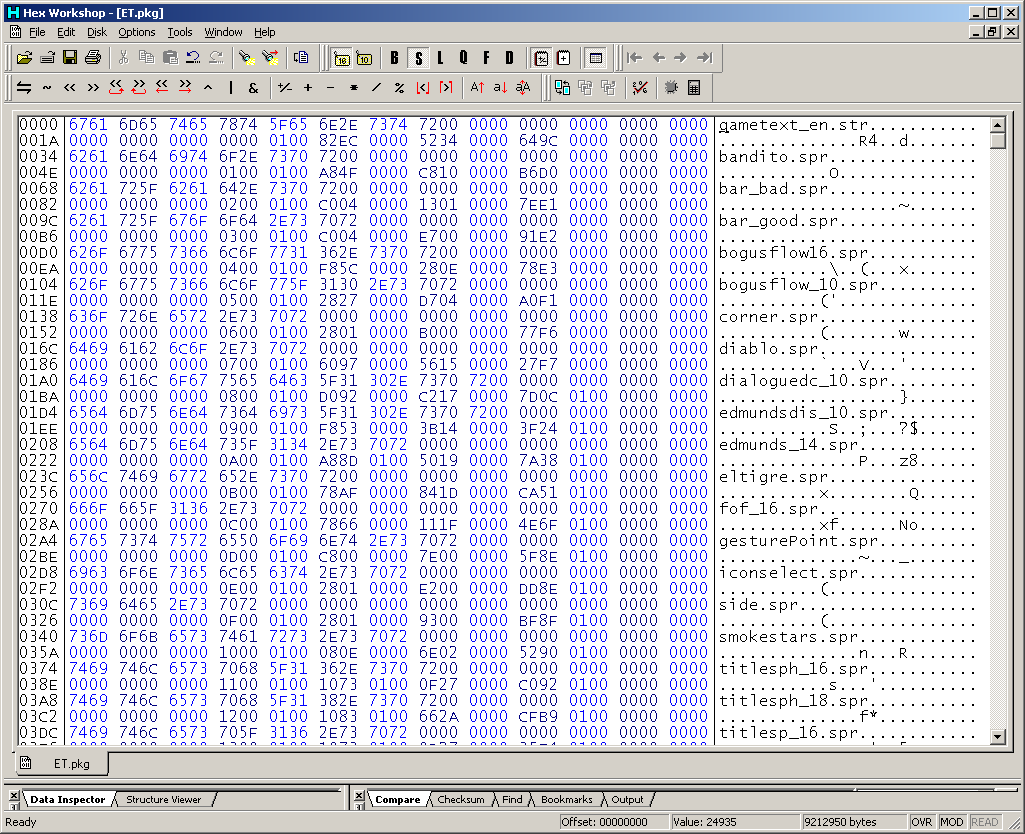
\includegraphics{images/19_home_fast6191_romhackingguide_unrenamed_file___borders_romhackingguidebasicfileformatshex2.png}
\caption{PIC}
\end{figure}

\hypertarget{graphics}{%
\chapter{Graphics}\label{graphics}}

Whether it is ripping them or wanting to edit them the field of graphics hacking is, and has long been, a huge part of ROM hacking. Generally there is a line that can be drawn between 2d and 3d imagery as they tend to have different hardware underneath it all, however both can be used in conjunction to influence and augment the other; isometric imagery and sprites used to generate a first person ``3d'' view is nothing new but many are surprised to hear that New Super Mario Brothers on the DS used 3d models instead of sprites to make a fairly traditional 2D platformer. The 3d hardware of the DS gets used in various ways that might not be immediately in line with the general perception of 3d as well.

\hypertarget{basic-graphics-concepts}{%
\section{Basic graphics concepts}\label{basic-graphics-concepts}}

In computer games, and most visual or other sensory media until you meet things like abstract works (note a somewhat different concept to abstraction as seen elsewhere in this document), there are two concepts that feed off each other at work. 1) is the suspension of disbelief and 2) is getting the audience to use their imagination. 2) is the subject of any good artistic tutorial but in the meantime think how a camera might pan away and use some audio cues rather than attempting to display violence or a good book will spend a lot of time setting a scene and describing things or otherwise describe situations compelling to humans. As it is very involved 2) is not really something that can be covered here other than to say it is well worth learning about, even if you are mainly a technical person, both in general and to help when you try to guess what methods will be used to achieve an effect. 1) however is much more of a scientific discipline, although to cover it in depth we would have to delve into various aspects of biology and psychology, so it gets covered. To make an image look real, assuming you want that sort of thing\footnote{It stems from robotics but there is a concept known as the uncanny valley which reads in brief ``As a robot gains more human like qualities then humans will react more favourably to it on an emotional level, this is until a tipping point is reached where the robot is fairly similar to a human but not quite and humans will start reacting less favourably, or even negatively, on an emotional level until the robot gets considerably more realistic (no small feat). At such a point the emotional reaction turns back towards the positive''. The idea has parallels throughout media and other attempts to emulate either a human or something that is seen in the real world. To this end going for ultra realism is not always the best bet.} , it

\begin{enumerate}
\def\labelenumi{\arabic{enumi}.}
\tightlist
\item
  Has to replicate enough colours that the human eye can not tell (this is typically taken to be about 24 bit aka 16.7 million colours, although those that edit images like to go to 32 bit (4294967296 values) so as to have more information to edit with and avoid having colours jump from to the other) and although the GBA and DS screen is 16 bit it can do the job if you do it right.
\item
  Has to have enough information, this typically means having a point and the point next to it not being distinguishable from one another (if you can see the points that make up the average image something has gone wrong). Now there are ways around this as the human eye is better at brightness (luminance) than colours and there is such a thing as empty magnification where you can blow things up/zoom in but no real new information will be gained, not to mention humans do not see ultraviolet so it tends not to be replicated in imagery. Indeed much of lossy compression is tasked with doing just this.
\end{enumerate}

The alternative to actual pixels and having 3d ultimately rendering into pixels is so called vector imagery. Vector imagery is named for the mathematical/graphing term called vectors and defines images entirely mathematically (for instance ``draw a square, line thickness 3 with a length of 4 at point 0,14'' can be scaled to any size with simple multiplication). Fonts on computers have used it for years and consoles have recently got into it (newer fighting versions of Street Fighter being noted for it) but it is quite rare to see in the end result of a console game, much less a handheld title. Still if you want to there are programs like \href{http://inkscape.org/}{Inkscape} that you can try out and attempting to render pixel art as vector imagery is quite a popular activity in certain circles.

\hypertarget{aliasing}{%
\subsection{Aliasing}\label{aliasing}}

Most screens in the world (and as far as games go it is mainly only the Vectrex that differed here) use a grid of pixels that can be individually set to various colours to display images. Rendering this out means a nice defined line can appear as a run of a couple of pixels and then appear to shift one pixel and then another run. The human eye is quite adept at picking this up, and, unlike certain other concepts in video and graphics, even when otherwise not trained to (see the example below) so techniques (known as anti aliasing) were developed to lessen the effect.

Example (might need to zoom in a bit)

\begin{figure}
\centering
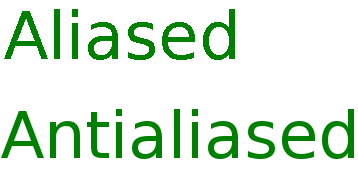
\includegraphics{images/20_home_fast6191_romhackingguide_unrenamed_file___iginal_borders_romhackingguidebasicaliasing.png}
\caption{PIC}
\end{figure}

This is also a problem when you take an image that was made at one size and scale it up, or sometimes when you scale it down, to something that is not a simple half (or quarter or so on) size of the original, beyond that though scaling non vector imagery has several potential pitfalls so do it sparingly or even better do not do it at all.

\hypertarget{haloing}{%
\subsection{Haloing}\label{haloing}}

Related in some ways to aliasing above, aliasing and the techniques to dodge it can trouble things. Here when trying to select just the outline of an item on a complex background it might be hampered by the anti aliasing which has a habit of causing a slight merging/smoothing of colours and transitions, as a result a coloured outline can appear around it which looks not unlike a halo. This is one of the reasons why sprite sheets and similar things will often come as a selection of sprites on a hot pink or lime green background which lessen merging effects.

\hypertarget{bit-depth}{%
\subsection{Bit depth}\label{bit-depth}}

In general imagery it means one thing and that is how many bits are assigned to colours, something which was covered in the introduction to this section, but in 2d console imagery it means what number is assigned to represent each pixel with typical values being 4 and 8, though 1 and 2 are seen commonly enough on various systems, including the GBA and DS. Now this does not mean 4 and 8 bit colours but that you can select from a choice of colours from a premade selection which is composed of 16 bit colours. Later on a concept known as ``sector addressing'' is covered which works on a related principle.

\hypertarget{palettes-and-colours}{%
\section{Palettes and colours}\label{palettes-and-colours}}

Although the GBA and DS capable of 16 bit (well 15 bit) colours you usually do not have the ability to define any number of 16 bit colours to use in a given image (remember tiles are like paint by numbers and you might only have 4 bits aka 16 colours at once or 8 bits aka 256 colours at once).

\hypertarget{gba-colours-15-bit}{%
\subsection{GBA colours (15 bit)}\label{gba-colours-15-bit}}

There is an undocumented feature on the GBA (and GBA mode of the DS) that swaps the green and blue but that is not that commonly used.

The GBA is said to be a 16 bit screen but as there are three colours used to make others each 16 bit value is in fact 15 with the 16th bit wasted.

Bits 0 to 4 deal with Red

Bits 5 to 9 deal with Green

Bits 10 to 14 deal with Blue

This allows 32 intensities (consider it a 5 bit number and higher numbers are more intense with lower ones being closer to black\footnote{The lower range until at least 10 decimal on the first GBA screens, and in some cases the later ones, are not so good so developers would often manually up the contrast or brightness for their games. This did not do well when the GBA SP arrived and which featured a frontlight, and later a backlight, as standard. To this end several people have hacked and continue to hack GBA games to improve the colours or, in the case of games with originals on the SNES (it also uses a BGR colour model) and such, port colours from the ``originals''. It should be noted Donkey Kong Country actually changed far more and downsized some sprites meaning it is not a simple hack to restore it.} ).

This also means that depending upon how you look at it the GBA/DS (and SNES) use BGR video instead of the standard RGB notation used almost everywhere else (naturally with printing using different primary colours to light it uses a different colour setup which is usually Cyan Magenta Yellow blacK hence your colour printer usually having four cartridges or ink level displays). The other method of note comes into play usually when video is involved and is known as yuv (which also leads to YV12) but that will be mentioned later and has no effect on any of the standard 2d and 2d imagery used on the GBA or DS.

In most operations the DS and GBA make a palette of various colours using the above method and the imagery refers to this to generate the colours. If you need to turn it into a 32 bit colour value, say for HTML colour notation, most of the time it is directly interpolated (multiply by 7.96875 which is 255 divided by 32) without correction, save maybe for a rounding (this can vary between implementations), and as most screens are not calibrated properly and the GBA/DS screens are not stellar to begin with it works well enough.

It should also be noted the DS has a master brightness section just before the image is displayed and optional capture hardware that change how an image ends up being displayed and this is in addition to some of the extra features afforded to the GBA and DS that will be covered later.

\hypertarget{tiles}{%
\section{Tiles}\label{tiles}}

Although you can draw an entire image on screen at once (many DS games are great fans of this and effectively make a tile 256 wide by 192 high necessitating a tile editor capable of handling it, a trick which many legacy ones are not able to) most 2d graphics are built from small building blocks known as tiles. Typically these tiles are 8 by 8 or 16 by 16 pixels although text fonts and 3d textures as well as the previously mentioned ``full screen tiles'' like to break from form here. The simple way to think about them is to think of them as very boring (thanks to the square pixels) versions of a paint by numbers picture with the numbers being looked up from a palette. Although most people never have to touch the graphics themselves with a hex editor an appreciation of how the hardware works is necessary to reverse engineer some of the more complex formats. Likewise to gain an appreciation for the animation/handling mechanisms learning about the methods by which tiles and palettes for them operate is all but mandatory.

\hypertarget{bpp}{%
\subsection{1Bpp}\label{bpp}}

Technically it is a compression method (the screen/video hardware itself does not display the mode in any real sense) but it is a special case as it is so simple that a basic tile editor can handle it and it can be edited in place without issue as indeed Crystaltile2 does, to that end it is here rather than later on when compression is discussed. The idea being if you have a black and white font or some other two colour image each four bits, the minimum length for a pixel the hardware accepts, will in fact be one or the other allowing you to compress the image down into 1 bit per pixel. Although it is not mandatory for developers to use it when dealing with 1bpp imagery the GBA and DS BIOS actually carry a ``decompression'' method in SWI10h that is known as BitUnPack.

\hypertarget{bpp-1}{%
\subsection{4 Bpp}\label{bpp-1}}

The workhorse of the GBA and a good chunk of the DS. Bringing back the icon from Yakuman DS. The ``marching ants'' selection is the section viewed in the hex editor which is as it is in the original ROM (certain hex editors can flip nibbles but it was not done here). As you can see each nibble looks up the value of a single colour (one of 16) which can be anything in the 15 bit format the GBA and DS can use. Equally there are 32 palettes each with the option for 16 colours which the game can swap between at runtime. Although not the only colour animation possible (the palette can also be edited at runtime) a developer can use these multiple palettes to change the appearance of items within the game and if you see the option to change at say the start of a battle (advance wars war room is good for this) or indeed at runtime then you are almost certainly looking at this.

\begin{figure}
\centering
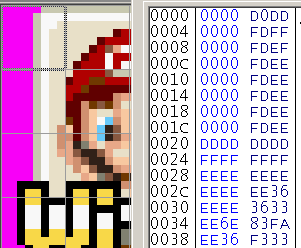
\includegraphics{images/0_home_fast6191_romhackingguide_unrenamed_files_and_original_borders_romhackingendiandemo.png}
\caption{PIC}
\end{figure}

Palette

\begin{figure}
\centering

\includegraphics{images/21_home_fast6191_romhackingguide_unrenamed_file___inal_borders_romhackingguide4bpppalettedemo.png}
\caption{PIC}
\end{figure}

As you can imagine the background is not pink in the real game and this is as the first colour in a palette is treated as though it was transparent regardless of what it is (although in practice is is fairly pointless with the way the screen works it allows for a full colour range without the loss of a single colour).

\hypertarget{bpp-2}{%
\subsection{8Bpp}\label{bpp-2}}

Although available and well used on the GBA it really started to be used on the DS.

Here each palette entry is 8 bits long and a two 256 colour palettes are available although only one for each mode (BG and OAM)

\begin{figure}
\centering
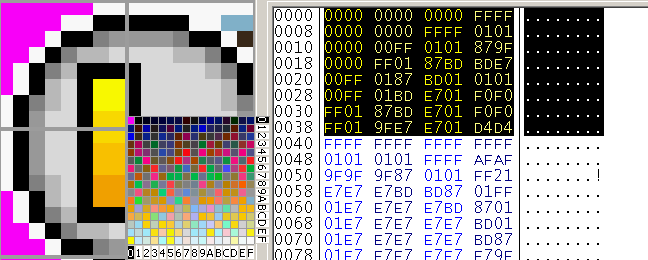
\includegraphics{images/22_home_fast6191_romhackingguide_unrenamed_file___inal_borders_romhackingguide8bpppalettedemo.png}
\caption{PIC}
\end{figure}

Here each hex digit is the lookup for the palette with the first being the row and the second being the column (although if you really wanted you could flip them and indeed the hardware probably does effectively just that but that is introducing completely unnecessary work for no real gain).

\hypertarget{gba3-xbpp}{%
\subsection{GBA3 Xbpp}\label{gba3-xbpp}}

There is another method that much like 1Bpp acts as a sort of compression meets hardware format method. Crystaltile2 is one of the few editors with support for this method and it is very rare indeed (the very occasional font being about the only thing that uses it).

It is a kind of 4 colour format (2 bits per pixel) but values are actually interleaved between two consecutive tiles.

Nibbles are ``flipped'' similar to the 4bpp GBA format. The order of the nibbles is then lower tile, upper tile, lower tile, upper tile\ldots\ldots{}

\textbf{A basic example of the interleaved format} 8x8 tiles (larger tiles of this pretty much follows the same pattern but to spare confusion it will not be covered here).

Palette as defined in the image. Remember the nibbles are actually flipped but ignoring that for the moment

\begin{figure}
\centering
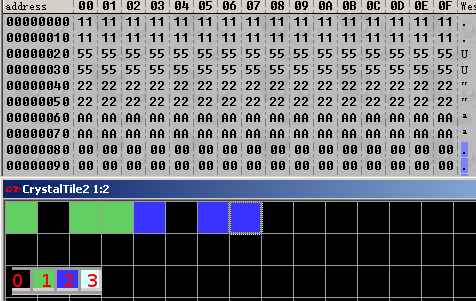
\includegraphics{images/23_home_fast6191_romhackingguide_unrenamed_file___original_borders_romhackingguide2dGBA3XBPP1.png}
\caption{PIC}
\end{figure}

The first pair of tiles is one fully green (01 binary on the palette) and one fully black (00 binary)

The second pair of tiles is both fully green (01 binary on the palette)

All this being said it is 4 bits between the start of a pixel in a given tile and the start of the next pixel in the tile which gives rise to the numbers seen

1 hexadecimal is 0001 binary hence the 00 going to the second (lower) tile and 01 going to the first (upper) tile.

The second pair is both green and is represented by 5 hex

5 hex corresponds to 0101 binary

The pattern still holds for the single blue and single black tile

The dual blue tiles

A hex corresponds to 1010 binary.

A more complex example Most of this is going to be left as an exercise to the reader but as mentioned the nibbles are flipped in a similar manner to 4bpp and it is not immediately apparent in the above example.

\begin{figure}
\centering
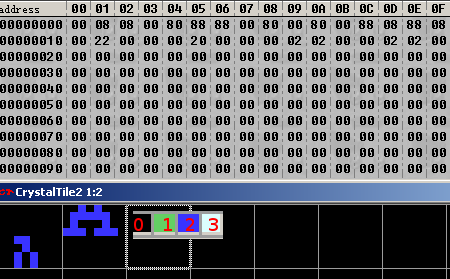
\includegraphics{images/24_home_fast6191_romhackingguide_unrenamed_file___original_borders_romhackingguide2dGBA3XBPP2.png}
\caption{PIC}
\end{figure}

The leftmost (upper) tile is blank for 4 vertical pixels but the lower tile has data in it.

00 08 08 00 hex

0000 0000 0000 1000 0000 1000 0000 0000 binary

80 88 88 00 hex

1000 0000 1000 1000 1000 1000 0000 0000 binary

The first pixel is blank on both counts as is the second so the 00 holds.

The third is not blank yet it is still 00, the fourth is blank but it is 10 (10 binary = 3 remember). As mentioned the nibbles are flipped with respect to the pixels they represent.

The fifth pixel is blue but it is 00 and the sixth pixel is 10 (again flipped).

Going to the next line

Blank and then blue. Flipped again (10 and 00 being seen in the binary).

\hypertarget{gba2-4bpp}{%
\subsection{GBA2 4BPP}\label{gba2-4bpp}}

For the sake of completeness crystaltile2 has another format known as GBA2 4bpp that is in some ways slightly more complex than GBA3 XBPP. Very few games have ever been observed to use it either.

It is a 4bpp format and technically is not nibble flipped like the other sub 8 bit formats but in practice it is a kind of interpolated format (each pixel technically having a choice of four colours) and additionally the first pixel in the pair of them sets the colour range for the second one.

The range in question is value 0-3, 4-7, 8-B and C-F. They could up so 0 through 3 allows the first four pixels (selection 0), 4 through 7 allows the second four pixels (selection 1) and so on but some more background is needed before that makes sense.

The first nibble selects from the first four colours using the range (0 through 3 pixel 0, 4 through 7 pixel 1 and so on)

The second nibble selects from one of four colours also in a row but what four it can select from is determined by the value of the first nibble. Within the values although it might not matter for the first pixel the second one has the four pixels also in a range of four and those are selected by the actual value within first pixel.

Examples

Selection 0 value 2 (in practice it would be 2 hex for the first pixel) allows the third group of colours from the palette for the second pixel.

Selection 3 value 2 (in practice it would be E hex for the first pixel) allows the third group of colours from the palette for the second pixel.

Selection 0 value 0 (in practice it would be 0 hex for the first pixel) allows the first group of colours from the palette for the second pixel (0 through 3 in the standard numbering).

\begin{figure}
\centering
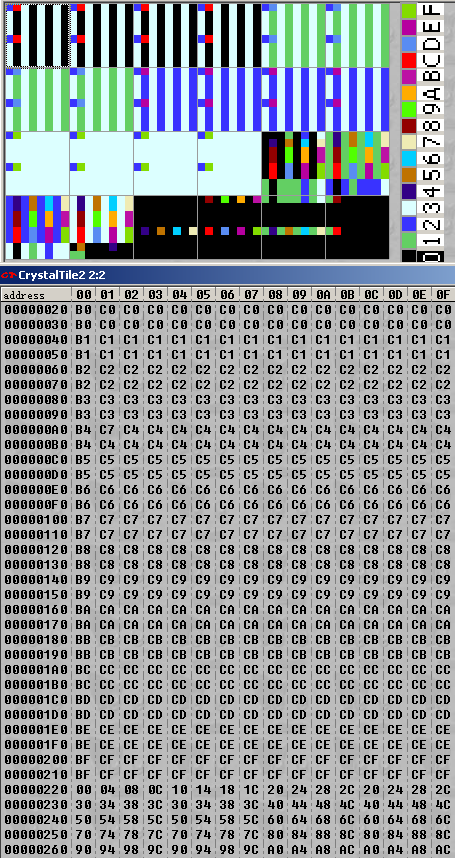
\includegraphics{images/25_home_fast6191_romhackingguide_unrenamed_file___original_borders_romhackingguide2dGBA24BPP1.png}
\caption{PIC}
\end{figure}

\hypertarget{bitmap}{%
\subsection{Bitmap}\label{bitmap}}

This will probably be better served after discussion of graphics modes and hardware but know this is not referring to the ``bitmap'' image format as seen in every basic image editor and most advanced ones, although some modes of it share a lot in common with said format.

The GBA has the ability to eschew tiles and just draw images line by line across the entire screen although it limits what can be done as to do it takes up most of the VRAM and it is not feasible to change it all every frame so extremely few games use it.

In the graphics it is known as modes 3, 4 and 5

3

is a 240x160 (aka the GBA resolution) 16 bit mode where colours are defined there and then (same BGR fashion as the rest of the hardware)

4

is a 240x160 8 bit mode where the full 256 colour palette is used (modes 3 and 5 do not allow transparent colours unlike this) and allows 2 frames to be defined in memory at once.

5

is a 160x128 (less than GBA resolution) mode using the same idea as mode 3 but the lowered size allows two frames to be stored in VRAM.

The DS has a kind of related tile mode where large tiles still composed or palette references like regular tiles can be used and it is quite popular but the DS has a slightly increased VRAM size to manage this better. It also has the ability to hold and manipulate images larger than the resolution in bitmap modes (it comes in handy for some end stage representation of 3d) although again this is better served for a discussion of hardware.

\hypertarget{known-formats}{%
\subsection{Known formats}\label{known-formats}}

Some games have been seen to use known/common formats like GIF, PNG and JPEG with the most prolific being that of the DS Opera browser. With it having to decode them as part of the general operation (what is the web without images after all) meant it could use such formats internally quite happily but other games have certainly been seen to do this as well. This becomes even more common on other more powerful consoles but the DS does have a few formats that Nintendo provides in the SDK that allow for some fairly extensive abilities, more on those in the layout/OAM section.

\hypertarget{crystaltile2-export-and-import.}{%
\subsection{Crystaltile2 export and import.}\label{crystaltile2-export-and-import.}}

Although Crystaltile2 usage is covered in depth later this is a basic operation and should be covered now. Most tile editors are just that and will allow you to edit an image but occasionally you are going to want to not be tied to a pixel by pixel editor and will want to use a more featured editor.

The act of exporting and importing images is easy enough. Although it is quite possible to do without a palette set properly it is best to have one in place else you will have to edit pixels accordingly in your proper image editor (red means blue and such) and much like hex mathematics you can fall foul of this when just making quick changes.

First select the tiles/area you want to edit. The either right click or click the edit pulldown menu

\begin{figure}
\centering
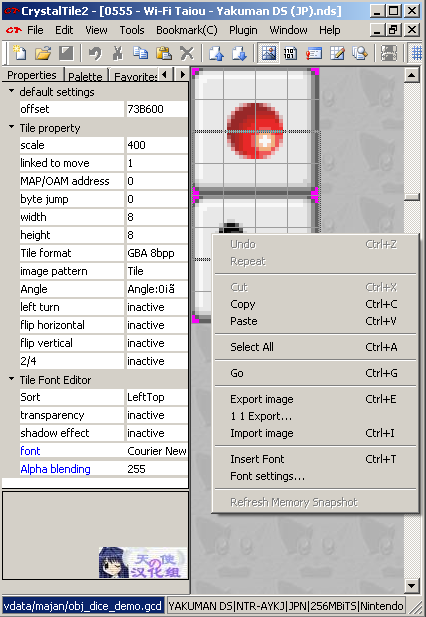
\includegraphics{images/26_home_fast6191_romhackingguide_unrenamed_file____borders_romhackingguidecrystaltile2export1.png}
\caption{PIC}
\end{figure}

You can either copy the image out if you have a few small edits but most will instead opt to export it. Crystaltile2 has a few basic options but BMP works for most purposes. Here you can import it into your chosen editor

There is also the second option of a 1:1 export which splits things along the tile lines and allows a sort of regular expression to be formed.

Once in the editor you can edit it accordingly

\begin{figure}
\centering
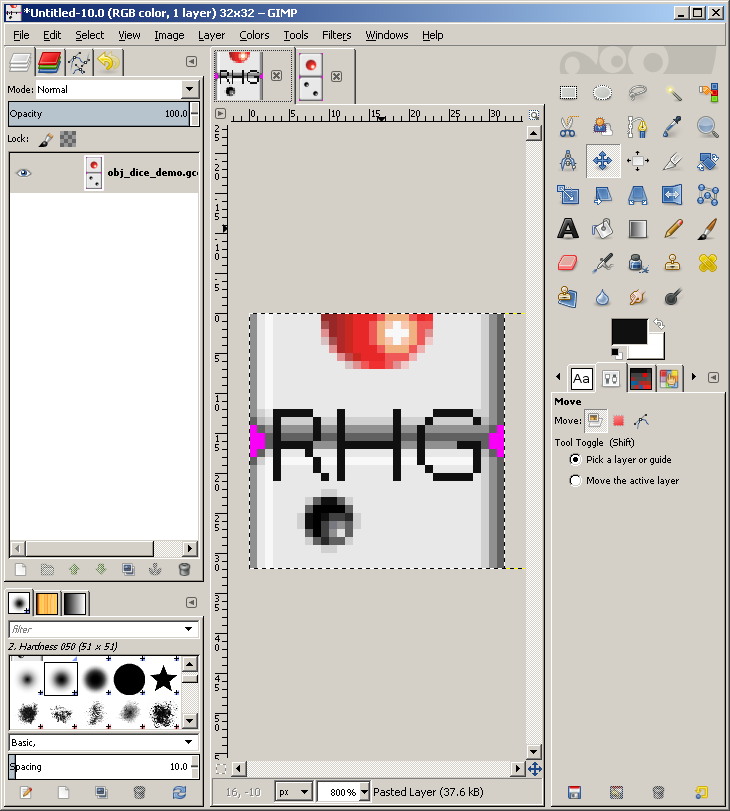
\includegraphics{images/27_home_fast6191_romhackingguide_unrenamed_file____borders_romhackingguidecrystaltile2export2.png}
\caption{PIC}
\end{figure}

Right clicking or clicking the edit pulldown menu and pressing import will import the newly saved image back into the editor where you can move it (it will snap to gridlines). Again you can use the copy and paste if you prefer although do remember to merge layers if your editor supports it.

\begin{figure}
\centering
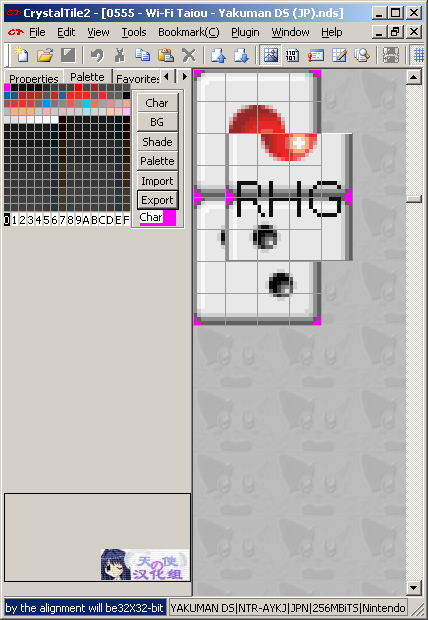
\includegraphics{images/28_home_fast6191_romhackingguide_unrenamed_file____borders_romhackingguidecrystaltile2export3.png}
\caption{PIC}
\end{figure}

Move it accordingly and then double click the image to set the image

\begin{figure}
\centering
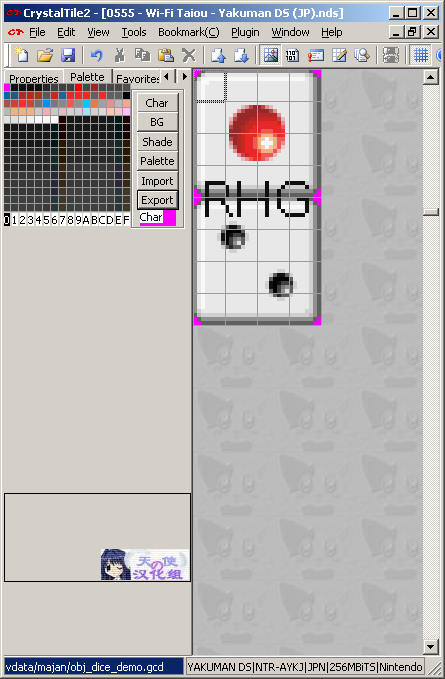
\includegraphics{images/29_home_fast6191_romhackingguide_unrenamed_file____borders_romhackingguidecrystaltile2export4.png}
\caption{PIC}
\end{figure}

\textbf{On palettes} If the colour you want is in the image then the dropper is usually sufficient but most tile editors have the option to export palettes to the commonly supported windows palette format; crystaltile2 has it right there in the palette window and BMP has a palette built into the file format (technically optional but crystaltile2 includes it).

\hypertarget{avoiding-gradients-aa-lossy-compression-noise-and-such-things.}{%
\subsection{Avoiding gradients, AA, lossy compression, noise and such things.}\label{avoiding-gradients-aa-lossy-compression-noise-and-such-things.}}

The name of this says it all really and most pixel artists will know this already, however it needs to be mentioned to spare you the hassle of having to redo the whole palette which might not even be viable if the palette is used elsewhere, not to mention if you only have limited colours available it makes sense not to waste them unless you do truly have the option to do so. To this end you should avoid gradients (hopefully one already exists if you need one), anti aliasing options (quite often added in when adding text), resizing (the nearest neighbour algorithm is probably the worst general usage scaling method but it has the benefit of using the colours it had to begin with if you truly need one), noise functions and other things that will add random extra colours to your image (like saving as JPEG, even at ``100\%''). This means that unlike most image editing you might have done at other points in life you are limited here.

On a different note much like changing palettes can change things elsewhere in the ROM you also have layout to contend with, or worse you face limited memory, which might limit the tiles you can edit but that is the subject of the next section.

\hypertarget{layout-timing-oam-and-special-effects}{%
\section{Layout, timing, OAM and special effects}\label{layout-timing-oam-and-special-effects}}

The consoles do not magically know how to sort tiles out and indeed much of 3d and 2d imagery, as well as coding in general, revolves around reusing things to lessen the drain on resources; you surely have seen old RPGs where you would fight a giant rat, a plague rat which looks exactly like giant rat but with a green and dark blue/purple paint job and later fire rat which has a red, orange and yellow paint job but looks exactly like the earlier rats. To do this the GBA and DS have hardware they can employ to change things in addition to the palette although said hardware can also control what palette is used. Most of the images used thus far have been simply one tile after the other and aligned manually for the purposes of clarity but there arises the concept of tile reuse which breaks the one after the other pattern and compositing (sticking one image over another) to trouble this, both are very common techniques in 2d imagery.

\hypertarget{introduction-to-the-oam-and-bg-modes.}{%
\subsection{Introduction to the OAM and BG modes.}\label{introduction-to-the-oam-and-bg-modes.}}

The GBA and DS have two principle graphics types known as ``BG'' aka background and ``OAM'' aka object area memory aka sprites which work together to display games. Although you can use one to do the other, and games have done as such, for the most part the distinction is observed and backgrounds will be left to do backgrounds (a big exception on the DS is 3d which is rendered in the 3d hardware and moved to the background to display) and OAM which is left to handle the sprites and image overlays (give or take windowing). Text can be in either BG or OAM depending upon the game although BG is far more common and usually the suggested method for developers to use. Finding out what method something uses is usually best done by getting to the point in the game it is used and viewing the OAM, sprite and BG in a given emulator (VBA for the GBA and desmume both feature such abilities). Such viewers are also a fairly good ripping method.

The GBA and DS are much the same although the DS has two engines known as A and B which is ostensibly one for each screen although they are not tied to a given screen and can easily be swapped at runtime. The ``A'' engine has more memory, the ability to do full VRAM bitmaps as well as what mainly houses the results of the 3d (engine B can use the results of the 3d but it requires some thought) and has use of the ``capture'' hardware which can be used to create effects although the more general general effects/functions still work on engine B.

As with most other things on the handhelds the hardware itself has sections dedicated to running various aspects of the hardware with graphics forming a large chunk of it. DS 3d aside there are two main components that go into video

• The main handler known as ``DISPCNT'' is found at 4000000 hex on both the GBA and DS (although the DS only has it on the ARM9 memory mappings and has a second one for the B engine at 4001000 hex).

• The actual BG (4 16 bit sections) and OAM stuff that handles all the lower level things for each of the various modes.

\hypertarget{timing}{%
\subsection{Timing}\label{timing}}

The graphics hardware tends to act as a timer for much of the rest of the system as far as software is concerned with a very significant component of the checks, updates and similar things being started when a vblank (vertical blank) happens.

The general idea is the screen is redrawn a scanline (a horizontal line across the screen) at a time. However after each scanline is drawn there is a pause known as hblank (equivalent to time taken to draw 68 pixels on the GBA) and after all the scanlines are drawn there is another pause known as vblank (on the GBA it works out to be about the time to draw 68 lines or just shy of 84000 cycles and the 71 lines for the DS means it is more or less the same refresh rate there). As updating the locations of things could cause tearing on the screen if it were done mid refresh any updates to the screen and other things closely related to it are triggered at these times (indeed the hardware itself dedicates the first couple of bits in interrupts solely to vblank and co). Either way the refresh rate is ever so slightly less than 60Hz which is why most games will aim for a framerate of just below 60FPS or half that at 30FPS.

Although knowledge of how the hardware works in this regard is definitely worth knowing about it should really be said that unless you are doing low level programming or are hooking into the code using timers based off it most of ROM hacking is not too concerned with it and more focus is put on the OAM, display registers and memory handling. The assembly section will cover more on interrupts but in the meantime if you do want to read more the\href{http://www.coranac.com/tonc/text/video.htm}{Tonc video section} has a nice worked example and \href{http://problemkaputt.de/gbatek.htm\#lcddimensionsandtimings}{GBAtek} has a lot of numbers.

Also as mentioned interrupts are a big thing so \href{http://problemkaputt.de/gbatek.htm\#gbainterruptcontrol}{GBAtek on interrupts}.

\hypertarget{gba-and-ds-oam-sprites}{%
\subsection{GBA and DS OAM (sprites)}\label{gba-and-ds-oam-sprites}}

Sprites (occasionally known as OBJs) are probably the main workhorse of games (they are typically the things you move, the game moves and you spend most of the game focusing on) and being able to manipulate them is a useful feature. The GBA supports up to 128 of them at any one time and each is given a section of memory.

07000000 hex is the location of the OAM on the GBA with obj 0 at 07000000 hex, obj1 at 07000008 hex obj2 at 07000010 hex, obj3 at 07000018 hex and so forth.

The DS is much the same but it has a second bank at 7000400 hex that is also 1 Kbyte long for engine B.

It gets quite complex and as not much beyond a basic appreciation of the concepts is necessary for most hacking work (if you have an appreciation for how it works, can look it up and with the help of the documents decode the values found that is good enough for most things), still you are referred to \href{http://problemkaputt.de/gbatek.htm\#lcdobjoamattributes}{GBAtek} which has a full listing if you want it.

Three 16 bit values make up most of the useful things and packed into each of those 16 bits

Attribute 0 - First 16 bits - Y coordinates (bits 0 to 7 leading to 256 options)

Attribute 0 - Second 16 bits - X coordinates (bits 0 to 8 leading to 512 options)

Attribute 0 - Third 16 bits - name, priority and 4 bpp palette selection

Priority is for each obj relative to the backgrounds and the lower values of objs have a higher priority relative to each other.

The other bits are used for rotation, flip, size and scaling options with the remaining 16 bits in the range used for the payload of the rotation and scaling functions when they are employed.

Most of the time edits to them are done manually with just a few tweaks or handled at function level when dealing with assembly but if you do need to edit them there are tools. Equally there are formats in the case of the DS that handle initial values/setup of it for various files so editing those is often more useful.

\textbf{OAM calculator for the DS} \href{http://filetrip.net/nds-downloads/utilities/download-oam-calculator-10-f29054.html}{Filetrip download}

If you need to edit OAM on the DS (it might also work for the GBA but be wary as a couple of things on the priority side of things are changed) or likewise decode a value you need not do it by hand thanks to this tool. Usage is fairly straightforward

\begin{figure}
\centering
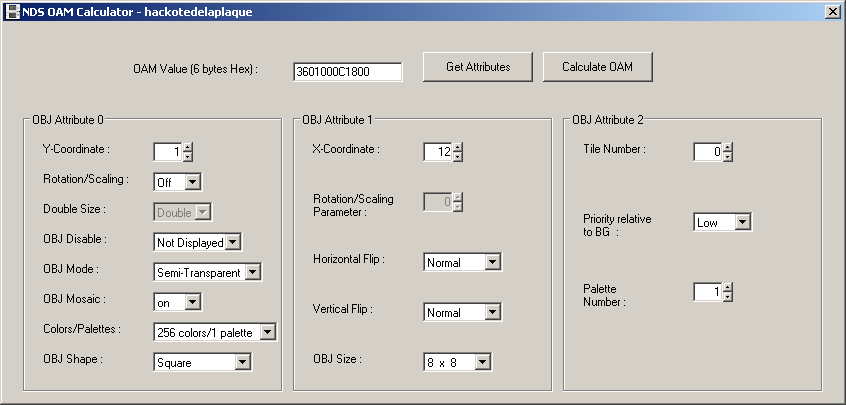
\includegraphics{images/30_home_fast6191_romhackingguide_unrenamed_file___orders_romhackingguidegraphicsOAMcalculator.png}
\caption{PIC}
\end{figure}

\textbf{Basic emulator view} This just has a quick example of viewing the memory (editing is sometimes possible here but often refreshed every vblank). From here you would trace the thing that originally changed the OAM and change things in the original binary (the DS quite often has helper formats for the graphics and the GBA was fairly good about keeping the actual binary code and the OAM values separate). It is also an early preview of animation via the OAM as well.

\textbf{GBA} VBA. The sprite here is actually made up of multiple tiles.

\begin{figure}
\centering
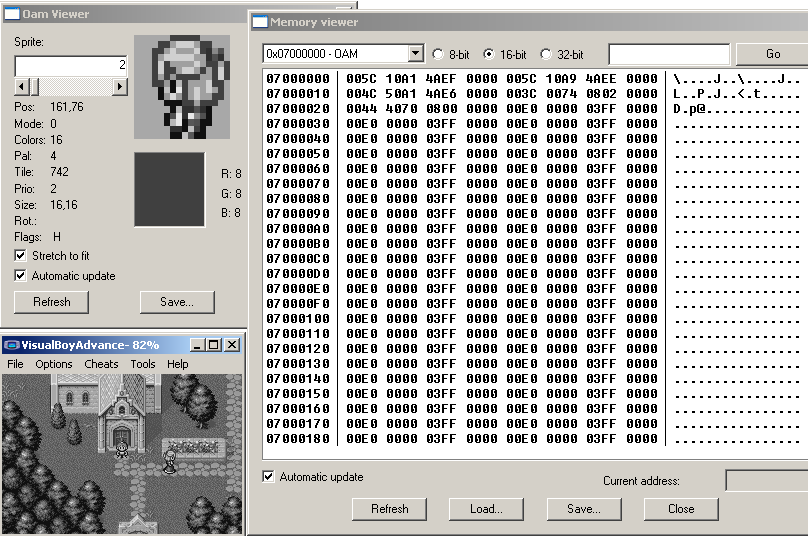
\includegraphics{images/31_home_fast6191_romhackingguide_unrenamed_files_and_original_borders_romhackingguide2dOAMvba_1.png}
\caption{PIC}
\end{figure}

\begin{figure}
\centering
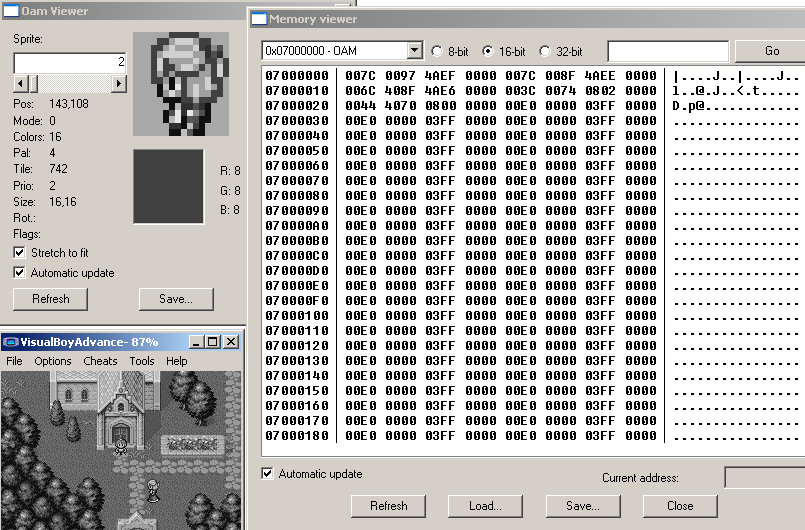
\includegraphics{images/32_home_fast6191_romhackingguide_unrenamed_files_and_original_borders_romhackingguide2dOAMvba_2.png}
\caption{PIC}
\end{figure}

DS Desmume.

\begin{figure}
\centering
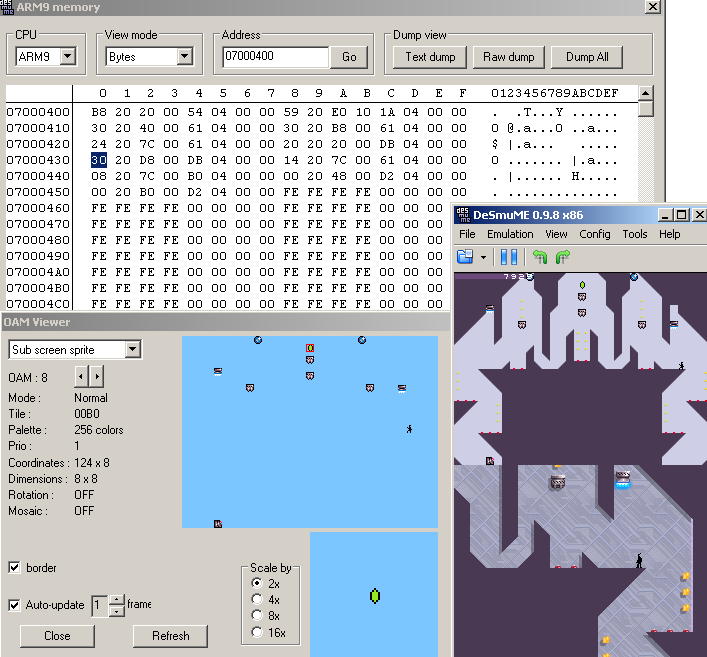
\includegraphics{images/33_home_fast6191_romhackingguide_unrenamed_file___ginal_borders_romhackingguide2dOAMdesmume_1.png}
\caption{PIC}
\end{figure}

\begin{figure}
\centering
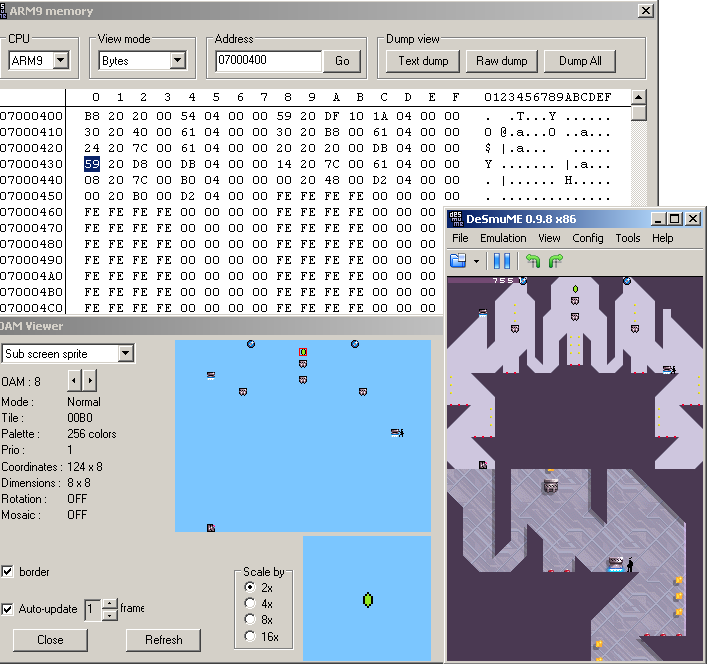
\includegraphics{images/34_home_fast6191_romhackingguide_unrenamed_file___ginal_borders_romhackingguide2dOAMdesmume_2.png}
\caption{PIC}
\end{figure}

\hypertarget{gba-and-ds-bg-modes}{%
\subsection{GBA and DS BG modes}\label{gba-and-ds-bg-modes}}

The BG modes tend to be for backgrounds, text and some menus, as well as providing the end result of the 3d rendering on the DS. On both the GBA and DS there are 4 backgrounds given the name 0 through 3 (again the DS has a second set of BG modes for engine B).

On the GBA there are 4 BG layers (0 through 3) and 7 modes, although different layers are restricted in what they can run. BG layers can be a higher resolution than the screen if given the right options/conditions and such things can be used for animation and general game usage to save having to stream content.

\textbf{How it works} There are two main options here for developers to use in games.

\begin{enumerate}
\def\labelenumi{\arabic{enumi}.}
\tightlist
\item
  Use a bitmap image
\item
  Generate a background from tiles
\end{enumerate}

The second is superior in most cases owing to the ability to do animations more easily (as mentioned previously the hardware is incapable of refreshing an entire bitmap each screen update) and as such is used by the majority of games.

\hypertarget{emulator-shots}{%
\subsection{Emulator shots}\label{emulator-shots}}

Most of the debugging emulators feature the ability to see the various layers that make a background. Typically this is called something like ``view map''. Examples of the VBA ones are present in the next few examples of other methods and it is much the same for any emulator with the only differences being in how much the hardware supports.

\textbf{Scrolling} The BG can be placed behind something and scrolled as a type of animation (often combined with other sorts of animation) or just have a larger BG section to focus the rest of the window on (there are other methods by which to have bigger ``rooms'' than the screen so do not assume this is how a game does it).

Visible in many games but an especially nice example exists in Tetris worlds for the GBA. From the same BG image the impression of random stars is given as a background.

\begin{figure}
\centering
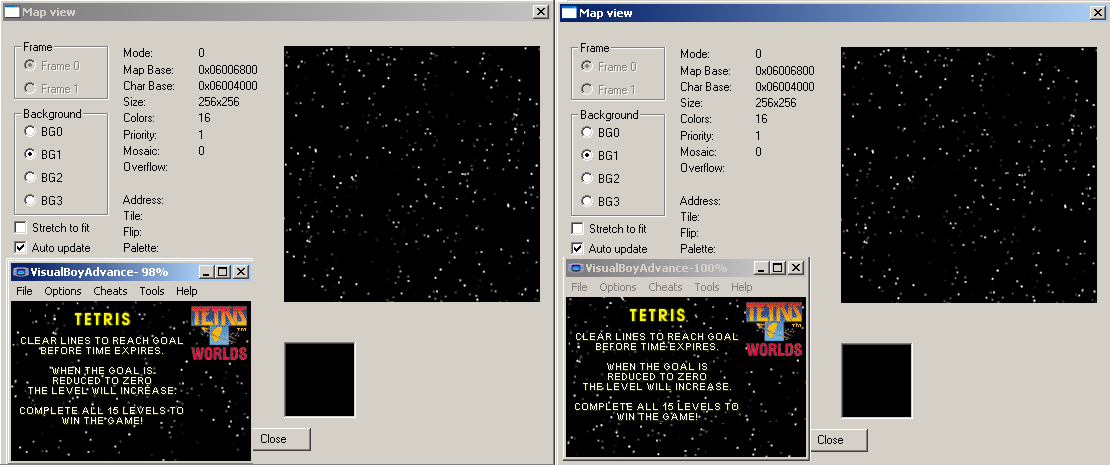
\includegraphics{images/35_home_fast6191_romhackingguide_unrenamed_file___inal_borders_romhackingguide2dBGscrolling_1.png}
\caption{PIC}
\end{figure}

Another good example exists in the first advance wars which actually makes use of the wrapping ability (see the lack of a complete Yellow Comet flag/logo)

\begin{figure}
\centering
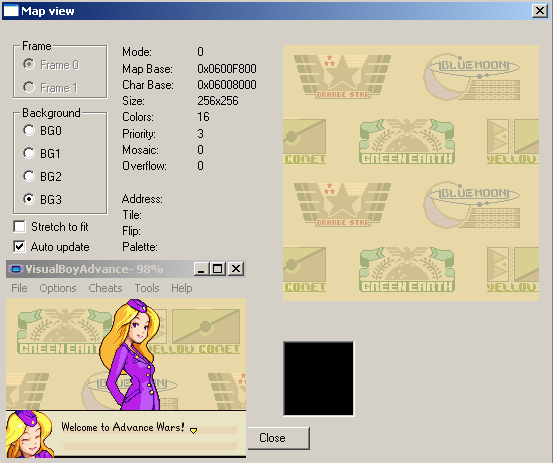
\includegraphics{images/36_home_fast6191_romhackingguide_unrenamed_file___inal_borders_romhackingguide2dBGscrolling_2.png}
\caption{PIC}
\end{figure}

\textbf{Layering effects} The classic example of this feature being used is beds in RPG games where the character will have a head visible above the pillow but the rest is covered. To do this there will be at least two layers with one being assigned a higher priority than the sprite and the second being assigned a lower one.

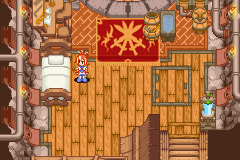
\includegraphics{images/37_home_fast6191_romhackingguide_unrenamed_file___original_borders_romhackingguideBGlayering1.png}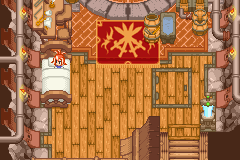
\includegraphics{images/38_home_fast6191_romhackingguide_unrenamed_file___original_borders_romhackingguideBGlayering2.png}

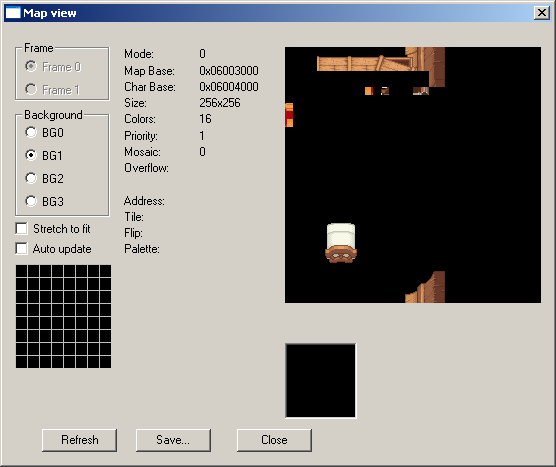
\includegraphics{images/39_home_fast6191_romhackingguide_unrenamed_file___original_borders_romhackingguideBGlayering3.png}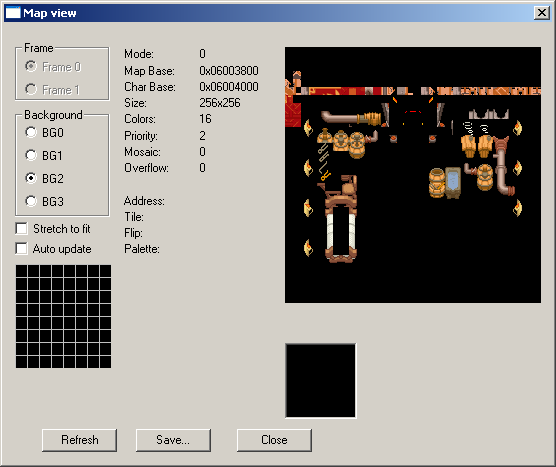
\includegraphics{images/40_home_fast6191_romhackingguide_unrenamed_file___original_borders_romhackingguideBGlayering4.png}

\begin{figure}
\centering
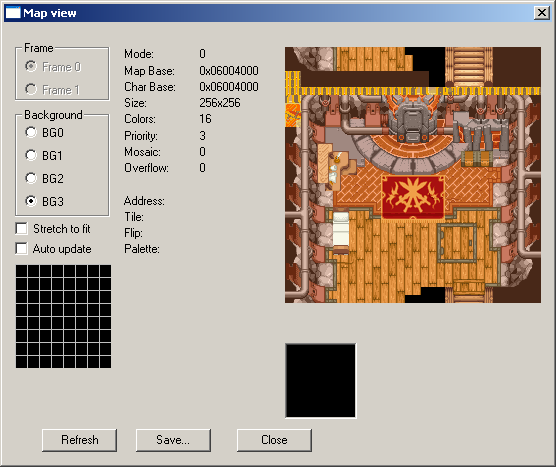
\includegraphics{images/41_home_fast6191_romhackingguide_unrenamed_file___original_borders_romhackingguideBGlayering5.png}
\caption{PIC}
\end{figure}

After disabling BG1

\begin{figure}
\centering
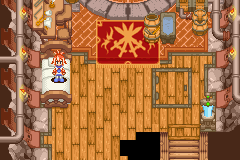
\includegraphics{images/42_home_fast6191_romhackingguide_unrenamed_file___original_borders_romhackingguideBGlayering6.png}
\caption{PIC}
\end{figure}

The second classic example which is slightly less involved is where trees or a structural beams will be placed over the game map allowing the sprites to move underneath them. Here many emulators will allow you to disable layers which can be useful when ripping maps to generate a game walkthrough.

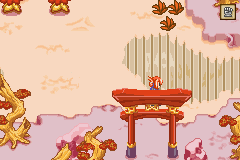
\includegraphics{images/43_home_fast6191_romhackingguide_unrenamed_file___original_borders_romhackingguideBGlayering7.png}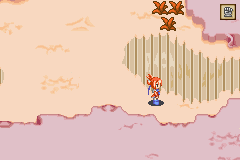
\includegraphics{images/44_home_fast6191_romhackingguide_unrenamed_file___original_borders_romhackingguideBGlayering8.png}

Example of beams from Phantasy Star 2

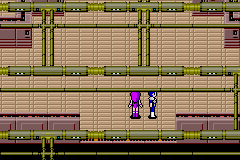
\includegraphics{images/45_home_fast6191_romhackingguide_unrenamed_file___original_borders_romhackingguideBGlayering9.png}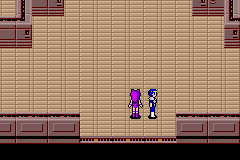
\includegraphics{images/46_home_fast6191_romhackingguide_unrenamed_file___riginal_borders_romhackingguideBGlayering10.png}

\begin{figure}
\centering
\includegraphics{images/47_home_fast6191_romhackingguide_unrenamed_file___riginal_borders_romhackingguideBGlayering11.png}
\caption{PIC}
\end{figure}

\hypertarget{basic-animation}{%
\subsection{Basic animation}\label{basic-animation}}

As the OAM can control what is on screen and where things are it is the thing responsible for most animation. There are additional abilities in rotating, scaling and such but those will be covered later. Although it is fairly obvious when seen from static images it should be noted that seeing it in real time is better so if you have the chance then do so.

There are concepts to consider.

\begin{enumerate}
\def\labelenumi{\arabic{enumi}.}
\tightlist
\item
  Screen movement
\item
  Sprite swapping
\end{enumerate}

As you will see later in video if you swap the images displayed on a screen fast enough it will appear to the human eye as though they are moving. This means you can swap sprites out to the relevant places after a given number of frames (the screen gets updated every vblank which is both the conventional and suggested point at which this is done). Combine this with movement of the screen or background and you get the impression of movement. Now, as you might have seen in the imagery representation section, images tend to be composed of multiple tiles so you do not have to swap an entire sprite set if you can swap swap the top half of a body instead and have the character throw their arms up as a result though this technique can go much further.

Formats will be covered in a few sections from here but the DS SDK does provide developers a fairly seldom used animation format known as NANR but moving back to the hardware there are several good examples of this in the Ace Attorney (Phoenix Wright) series.

Dragon Quest Rocket Slime The game provides a great example of OAM animation in the pre title screen sequence. Again if you can see it in real time it is quite a lot clearer.

\begin{figure}
\centering
\includegraphics{images/48_home_fast6191_romhackingguide_unrenamed_file___ginal_borders_romhackingguideOAManimation_1.png}
\caption{PIC}
\end{figure}

\begin{figure}
\centering
\includegraphics{images/49_home_fast6191_romhackingguide_unrenamed_file___ginal_borders_romhackingguideOAManimation_2.png}
\caption{PIC}
\end{figure}

\begin{figure}
\centering
\includegraphics{images/50_home_fast6191_romhackingguide_unrenamed_file___ginal_borders_romhackingguideOAManimation_3.png}
\caption{PIC}
\end{figure}

\textbf{Original Phoenix Wright animation} The above was plain animation via OAM but games occasionally get more interesting.

The first Phoenix Wright game had some fairly notable character animations but rather than redrawing each frame of the animation the characters themselves were actually split into components (usually face and hands) and those swapped out as necessary to create animation. The tile view is not quite how the internal formats do it (those usually being set up to take advantage of the hands and face being one visual concept).

\begin{figure}
\centering
\includegraphics{images/51_home_fast6191_romhackingguide_unrenamed_file___nal_borders_romhackingguideOAManimation_2_1.png}
\caption{PIC}
\end{figure}

\begin{figure}
\centering
\includegraphics{images/52_home_fast6191_romhackingguide_unrenamed_file___nal_borders_romhackingguideOAManimation_2_2.png}
\caption{PIC}
\end{figure}

\textbf{Background animation} The scrolling effect was mentioned already but if you are using a tiled background you can change the tiles the make up the background and create animation there. Animations with bitmap images has often been done on a programming basis but much of that is either very obvious or quite arcane and steeped in programming methods.

Another use of the scrolling effect is more commonly used as camera animation in 3d imagery but here if you rapidly move around the BG map a ``camera shaking'' effect is created and is well documented/entrenched in cinematography as something seen when a character or location is startled or hit.

\textbf{Palette animation} It has been mentioned briefly in the past but there is also the matter of palette animation aka dynamic palettes to consider as well. Here the game will change a colour or a handful of colours in the palette and this has a corresponding change in the main game.

From Summon Night Swordcraft Story 2 a quick sample of three stages of an animation. Changing parts of the palette have a black square added around them.

\begin{figure}
\centering
\includegraphics{images/53_home_fast6191_romhackingguide_unrenamed_file___rs_romhackingguidegraphicspaletteanimation1.png}
\caption{PIC}
\end{figure}

The game, unlike most on the GBA, also features a few different colour modes for the original GBA, GBA-SP, TV and the option to change brightness on a slider.

\textbf{Developer tricks} There is more on this in part III but some on 2d for now. The idea here is the developer will do things to make the demands on system resources less and in doing so allow them the potential for a larger amount of other things to be done which is always good.

For instance a character walking left is much the same as a character walking right so you only need to animate one direction and flip the sprites over. This might also trickle down into the sprite itself which will not be seen holding a weapon or something that will mark it as a flipped sprite.

If an area of a level is not being seen at present there is no need to animate it. The basement/smithy of the Summon Night Swordcraft Story 2 used in the palette animation section provides a great example. The 3d equivalent of this is backface culling and viewpoint rendering.

Another effect commonly seen in 3d animation but still useful in 2d, and seen in several games, is the addition of a single dark circle as a shadow.

\hypertarget{window-feature}{%
\subsection{Window feature}\label{window-feature}}

Although you can fill the whole screen the GBA and DS have abilities to pick and choose things to show and the technique is known as windowing. The basic idea is the mode is triggered which selects a region (you have two windows allowing for a four way split if you prefer) and you can change the display of BG and OBJs within it. Various things and games can employ it in the actual game but menus are a common usage.

\href{http://problemkaputt.de/gbatek.htm\#lcdiowindowfeature}{GBAtek windowing feature} explanation/description. The feature first has to be enabled in the DISPCNT register and then has the windows defined in other registers which can then have various BG or OBJ layers disabled as appropriate but do remember that transparency can be made to work for the BG so do not always expect windows to be used.

An animation technique can be done here and henke37 noted that things can be tweaked on hblank to create certain effects beyond the obvious classical or offset windows with \href{http://www.youtube.com/watch?v=1t8wWnI_I1I\&feature=related}{ghost trick (see around 5:20)} providing a nice example.

\hypertarget{special-features-flipping-affine-transformation-alpha-and-such}{%
\subsection{Special features (flipping, affine transformation, alpha and such)}\label{special-features-flipping-affine-transformation-alpha-and-such}}

Despite all the limited memory and quirks the GBA and DS or perhaps because of it both feature all sorts of methods that developers can employ to perform various alterations to the images seen.

\textbf{In OAM transformation} Mentioned briefly a few paragraphs back the OAM has options to flip sprites and individual tiles. and is quite often used to have characters walk to the left or walk to the right despite using a single set of sprites (you can see an example of it up in the GBA OAM viewing section). Double size is also available although intended use seems to be for working around affine transformation induced issues (preventing parts from being clipped off when rotated in most cases) rather than the immediately obvious (although that works as well).

\textbf{Affine} Many guides and documents will refer to this by the two most common things it does, which are the other two big transformations done to geometry known to most as rotation and scaling (the third one, translation, being fairly well taken care of by everything else). Strictly speaking though it does allow for shear transformation and some other things and so the term affine transformation is more fitting.

In the case of sprites/objs it is split across the first two attributes and the fourth hidden ones. The s in ones is not a typo as the normally unusual 4th attribute is in fact affine transformation data but it allows for 32 attributes (somewhat less than the 128 objects possible but that is not so bad as there is nothing stopping things from sharing a set of attributes) in all as the first four hidden attributes are used for a single transformation value and this is repeated.

Attribute 0 activates the mode

Attribute 1 selects the transformation grouping in bits 9 to 13.

The hidden attribute 3 is in fact split over four hidden attributes as mentioned and each carries one 16 bit value (signed 1 bit sign, 7 bits integer, 8 bits fraction format) corresponding to what are known as PA,PB,PC and PD which can be used to effect rotation, scale and shear transformation and all the same time if necessary (it does not quite work like it but if you imagine having control of every corner and how you can use that to scale things, shear things and rotate things at the same time) .

\href{http://www.coranac.com/tonc/text/affine.htm}{Tonc} has a worked example of a lot of the maths involved (in many ways it is as complex as maths in ROM hacking gets outside of some very in depth assembly hacking), it also returns after a fashion for the 3d system. It will be returned to there in earnest as it underpins the entire 3d system.

For those used to the maths the reference point is the top left of the object rather than the screen and the rotation centre is set as the middle of the sprite. In some ways this is quite limiting as some interesting things can be accomplished with different origins and centres of rotation but it does serve to simplify things for basic transformations.

\href{http://problemkaputt.de/gbatek.htm\#lcdobjoamattributes}{GBAtek} has basic listings and \href{http://www.coranac.com/tonc/text/affobj.htm}{tonc} has more worked examples.

BG affine transformation is slightly more involved but follows much of the same logic, \href{http://problemkaputt.de/gbatek.htm\#lcdiobgrotationscaling}{GBAtek} has more.

\textbf{Mosaic} Usually seen as the single corner pixel repeats for every unset pixel in the rest of the screen but it is available for smaller values. Has to be enabled in the individual control register and then set accordingly in 400004C hex but is available for all the BG layers as well as equivalents for sprites. \href{http://problemkaputt.de/gbatek.htm\#lcdiomosaicfunction}{GBAtek mosaic} section and \href{http://www.coranac.com/tonc/text/gfx.htm\#sec-blend}{Tonc} has some nice worked examples.

\textbf{Alpha and brightness} Alpha blending is a method by which two images can be merged together, the not entirely accurate but layman's equivalent term being called transparency, and can be used to achieve a variety of effects. Note that the DS 3d system has a rather more complex setup for alpha depending upon textures used and more.

For the most part alpha is a flag and variable which is to say if it wants to be alpha blended there will be a flag to say so and somewhere else a variable to say by how much (this is also where the 3d differs slightly in some modes).

Brightness adjustment, which the DS has a special mode in the capture unit for, is also possible with it being available instead of alpha if you want it. Note that many developers instead chose to alter brightness at the palette level for the original GBA model hence the hacks to restore colours that looked rather washed out in later GBA models.

Three registers are used here with 04000050 hex aka BLDCNT being the main select this mode 4000052 hex aka BLDALPHA being the alpha modes and 4000054 hex aka BLDY doing for the brightness. Note that although sprites can be blended here the setting can be overridden to always blend in the OAM.

\href{http://problemkaputt.de/gbatek.htm\#lcdiocolorspecialeffects}{GBAtek} has more depth and full listings.

\textbf{Mode 7} The SNES (which the GBA owes a lot to in terms of abilities and hardware design) was one of the first to allow for a perspective transformation of an image. Though now looking quite poor to those used to modern 3d imagery it was revolutionary at the time, so much so the hardware term from the SNES became shorthand for the technique. \href{http://www.coranac.com/tonc/text/mode7.htm}{Tonc} has more.

\hypertarget{basic-ds-layout-formats-and-mapping}{%
\subsection{Basic DS layout formats and mapping}\label{basic-ds-layout-formats-and-mapping}}

Although games and indeed many games do use raw formats and declare what they should be rendered as/mapped to elsewhere (or just have a tile for every tile on the screen) the nitroSDK provides several formats for developers to use. They range from simple wrappers for a layout to full animation formats. Also worth noting is that if an image is composed of tiles some of those tiles might be reused as a kind of compression so you might have to edit those (this is very often the case in Japanese puzzle games where text is part of the image and the two kanji can afford to have a blank tile in the middle).

A basic demonstration of the compression/tile reuse concept

\begin{figure}
\centering
\includegraphics{images/54_home_fast6191_romhackingguide_unrenamed_file___ginal_borders_3wizardozndsdemohack13jul2011.png}
\caption{PIC}
\end{figure}

A few clicks later

\begin{figure}
\centering
\includegraphics{images/55_home_fast6191_romhackingguide_unrenamed_file___ginal_borders_7wizardozndsdemohack15jul2011.png}
\caption{PIC}
\end{figure}

\textbf{Palette formats}

\textbf{NCLR}

Occasionally seen as RLCN it is a palette format. Most of the time a fairly pointless wrapper for the palette but other times does act as an archive format.

\textbf{NTFP}

Technically part of the NCLR format but seen quite often by itself and especially on earlier games.

\textbf{.PAL}

Not always a palette (it still being the shorthand for European and Australian TV standards and so versions of games aimed at there will sport that extension) but quite often palettes are seen with this extension.

\textbf{Tile storage} Tiles themselves need to be stored and various archive formats have been made for them

\textbf{NCGR}

A format that includes all the relevant data about the data stored (widths, heights, colour depths, whether it is tiles or not and more). Aimed more at sprites/objs but remember full screen images are possible and still used for BG type images.

\textbf{NTFT}

Another raw format that is technically part of another (in this case NCGR) but seen by itself on occasion.

\textbf{NSCR}

Aimed at background (BG) images and contains information on how to decode and set things up.

\textbf{NTFS}

Once more part of a bigger format (NSCR in this case)

Mapping Mapping merely involves arranging the OAM or BG into the proper order. It can be done in many ways but the nitroSDK provides a handful of methods although many are encompassed either by animation or by the storage methods themselves.

\textbf{NCER}

Aimed at sprites and provides initial OAM data among other things.

\textbf{Animation}

\textbf{NANR}

An infrequently used animation format.

\textbf{NMCR}

A format seen in pokemon to provide animations. In some ways it might be considered a wrapper to NANR.

Fonts It will be covered later in the text hacking section but there is a fairly complex font format many DS games use. Many other games use equally complex formats where others might use simple plain tiles (maybe in a slightly odd size).

\textbf{NFTR}

A font format the includes character widths/dimensions, line locations and various types of mapping available.

\textbf{General observations} Most DS editing programs will feature editing abilities for these formats and related ones and exporting and importing should not be a problem. However if you are after a more general image editor and have one that supports the Susie plugin format (a fairly popular plugin format seen in a lot of Japanese image editors) loveemu's \href{https://github.com/loveemu/nitroscrap/releases}{nitroscrap} heads down such a path.

Although they can and frequently are found by themselves they might be put into basic container formats like narc, custom ones as will be covered several times over during the course of this guide, occasionally stripped of components of (maps being ignored and such), be stripped down to the their basic components (basically a headerless file), have a single palette for an entire range of images (often this will be named accordingly but not always and either way it can confuse programs that expect the same name, which is most of them). This is especially true of animation which rarely uses the NANR format.

The formats have remained largely static over the course of things although pokemon has a habit of changing a few things, using rarely used features and reworking some others so tools built to earlier standards might not work properly with that franchise.

The names above are the extensions the files that carry them usually have but they are occasionally known by the magic stamp which is usually a reversed version of the extension (NCLR=RLCN and such).

In the absence of the formats at the end of the document

\href{http://llref.emutalk.net/docs/}{Lowlines current specifications}

\href{http://www.romhacking.net/documents/469/}{Lowlines older specifications}

\href{https://github.com/pleonex/tinke/tree/master/Tinke}{Tinke source code} (trunk/ Tinke/ Imagen and trunk/ Plugins)

\href{http://nvwr.googlecode.com/svn/trunk/libs/formats/}{Nintendo VieWer source code (python)}

They are largely aimed at programming with the latter two being source code to various programs.

\hypertarget{video-memory-handling-and-alignment}{%
\subsection{Video memory handling and alignment}\label{video-memory-handling-and-alignment}}

The GBA and DS video systems are quite in depth which serves both to work around issues of low power and to provide developers the options to do things they might otherwise have to spend a lot of time programming. One of the more interesting aspects of this is the memory handling as it is quite possible to run out and there are other quirks such as alignment.

2d memory management Games, especially on the GBA but the DS is no easy street, frequently push up against the limits of the memory and this means there is certainly not so much of it you can never run out and with certain graphics modes it is very easy to do. As ROM hacking so often wants to add things you will probably brush up against this eventually. The most common scenarios are you have a 2d overlay on a background and either the repeated tiles want to be edited or you want to extend the overlay a bit and run out of memory that way.

\href{http://pineight.com/gba/managing-sprite-vram.txt}{pineight.com}details a streaming method homebrew programmers can use to hopefully never run out of ram. DS programmers are not quite so fortunate and will tend to have to fiddle with maps and tiles or accept a slightly lesser image.

\textbf{Alignment} In short the GBA VRAM will only accept writes to values aligned to 16 bits and this most commonly rears up when compression is being dealt with. It has had such an effect that it led to a whole class of methods being described as VRAM safe or otherwise WRAM safe if they do not work on VRAM. Unless you are physically managing the VRAM as part of a hack (and not say relying on a function to read so much from the cart into it) it is usually just a matter of making sure you select the ``VRAM safe'' compression function of whatever program you are using.

\hypertarget{d}{%
\section{3d}\label{d}}

Although some games on consoles are experimenting with vector images between tiles and 2d above and 3d covered in this section the vast majority of imagery use in games is covered. Note it is far from unheard of for games to use their 3d hardware to display 2d imagery and animation (several title screens on games have been seen to do this at various levels and even swapping out 3d for conventional 2d at points), it was already mentioned how several apparently 2d games have used 3d models in place of sprites (New Super Mario Brothers being noted for it) and others have augmented 2d imagery by doing things like having backgrounds rendered on the 3d hardware (various reasons but mainly that it really troubled the nascent DS emulation scene finds the first Castlevania game being noted for it).

For the most part this section will be very basic general concepts and DS specifics as the GBA lacks proper 3d hardware and anything there is likely to be prerendered and given to the 2d, a trick like isometric imagery or ``mode 7'' style techniques. This section will also assume a knowledge of GBA/DS 2d hardware and can be considered to follow on directly from it.

On computers and to a lesser extent consoles as well (although they use the hardware designed for it the software development kit developers will often still cook up their own programming methods for it) the two dominant methods for rendering 3d at time of writing, and for some time prior, are known as DirectX (a 3D technology from Microsoft and used in Windows and the xbox line of consoles) and OpenGL (a 3d technology of similar power and scope but as it is relatively open it is used in most other places as well as being available for use in Windows).

Lines are blurred between the hardware running things and the standards built on top of them; DirectX and OpenGL will put standards out which the hardware makers will build to and the hardware makers (and engine developers) will also have a say in what should go in the next versions of the DirectX and OpenGL standards with it only getting more blurred as those technologies also start to encompass general computing tasks (physics and such for games but owing to the way they are built they are also pretty good for aspects of high performance computing) with GPGPU being the term of choice to look up. Also in the case of DirectX the standard also defines input methods and helps with sound.

For the most part though the GBA and DS have all that 2d animation capabilities that consoles or 2d animation in general ever wanted (naturally support for larger amounts of sprites and such, being faster and operating at higher resolutions are desirable) the DS 3D systems are not that much like current 3d systems or even that much like past ones. Basically if you knew all that was to know about GBA 2d and underlying methods you could do 2d anything but knowing all there is to know about DS 3d and the underlying methods will leave a large gap in your knowledge (the idea of shaders, much of light reflection and some of the ideas that have led to shortcuts/approximations are at best going to be touched upon) although it should not do a disservice to any future intentions to learn 3d imagery. Learning 3d imagery is quite possible thanks to the internet and \href{http://www.youtube.com/playlist?list=PL6A7DF3D7866EB076\&feature=plpp}{The Guerrilla CG Project} put out a nice series that covers a lot of the basic concepts.

\hypertarget{basic-3d-bones-coordinates-keyframes}{%
\subsection{Basic 3d (bones, coordinates, keyframes)}\label{basic-3d-bones-coordinates-keyframes}}

You can do 3d imagery in a lot of different ways and for the most part 3d and the way 3d is animated is not really possible to separate. In practice it comes down to keyframes which have quite a lot in common with their 2d counterparts, morphing which is a hybrid of keyframes and the following and bones which as the name implies a bunch of jointed (often imaginary) lines running through a character that can be moved to provide animation (lesser systems using fewer bones and joints and winding up with things like hands always in a ``pistol'' grip).

Coordinates. For the most part the X, Y, Z coordinate (Cartesian) system appears once more although with two main refinements either in hardware or when doing maths on them.

\begin{enumerate}
\def\labelenumi{\arabic{enumi}.}
\tightlist
\item
  The ability to define a line with an angle and a length
\item
  The ability to have a coordinate system within a coordinate system (helps when you have a complex shape and do not want to have to worry about recalculating a lot of points despite them not changing relative to each other).
\end{enumerate}

Angles and lengths are quite useful as they can be manipulated somewhat more easily in some ways (the general idea is a line is defined at the origin with an angle to the given axes and a length and then maybe translated which gives the same information as a set of coordinates but allows easier rotation and more). Strictly speaking it is not used in the hardware but it often feeds into the multiple coordinate systems.

Multiple coordinate systems are extremely useful once you get past basic 3d for as mentioned they allow you to rotate an entire shape and not have to worry about recalculating all the components within it and deal with odd angles not to mention it allows for independent animation. For instance consider your hand when curling your arm it is at the end of your wrist but if you curl your arm leaving the hand in the starting position and then try to map the coordinates your hand just passed through it gets horribly complex despite your hand not changing position relative to your wrist.

In most games made points are defined which then become the corners, or more accurately vertices, of a model and lines drawn between them to make the image and those points moved accordingly (usually via the bones technique) although the latest techniques at time of writing are experimenting with a technology known as geometry shaders where new lines can be generated after an explosion or something. Back on topic most of the time this line is straight although some more advanced systems can define a type of line to make for a curved image (other times you see this it can be textures though) which usually falls under the remit of subdivision although there is a lighting trick known as Gouraud shading that achieves a similar effect.

Another type of imagery seen mainly in 3d scanning (medicine and parts of reverse engineering devices) and certain types of computer modelling (usually scientific in nature) is known as point cloud data where individual points are used and expanded from there. As you might imagine this can be very costly in terms of resources which for more real time use leads to voxels where a image is composed of small boxes or if you prefer the points themselves expanded so as to meet their neighbours and can be seen in \href{http://voxelstein3d.sourceforge.net/}{voxelstein3d} among other things.

Optional maths lecture on arrays/matrices Arrays are a concept that arises early in discussions of 3d and programming in general and as they have some very useful functions they never really go away. With one though you can effectively define in a few numbers a primitive anything really; a 3 x 3 array stores 9 values which works quite well when you have an X, Y and Z value and three sets of those can define a triangle (the building block of most 3d images) and more although the DS favours 4x4 for a lot of things (even if it turns those 4x4 into 3x3 by setting all the but the bottom right coordinate to 0 and the bottom right one to 1.0) and does not use them for defining vertices per se but the model format might well store things in one. The underlying maths is not hard it is just not as most people that have previously spent time doing algebra immediately expect. For some of the more in depth 2d affine transformations the same maths and many of the same concepts will arise.

Both \href{http://problemkaputt.de/gbatek.htm\#ds3dmatrixexamplesmathsbasics}{GBAtek} and \href{http://www.coranac.com/tonc/text/matrix.htm}{Tonc} have more on this with the latter aimed at the GBA 2d.

Still there are a few select concepts worth knowing

\begin{itemize}
\tightlist
\item
  Dot product
\item
  Cross product
\item
  Scalar multiplication
\end{itemize}

Depending upon your point of view scalars are either regular numbers or a 1x1 matrix.

\[To finish\]

\textbf{The decimal point} Floating point was covered back in the introduction and it is surely not hard to see what the ability to represent numbers after the decimal point is useful in 3d modelling. Combined with the need to do operations on lots of data all at once (a problem ``solved'' by the introduction of \textbf{S}ingle \textbf{I}nstruction \textbf{M}ultiple \textbf{D}ata/ SIMD instructions) this is why 3d tends to have a piece of dedicated hardware inside the system and systems will have their performance measured in FLOPS (floating point operations per second). The DS specifically tends to eschew floating point in favour of fixed point using a variety of different formats for fixed point depending upon the operation.

A couple of different fixed point methods are used depending where you are

1bit sign, 3bit integer, 12bit fraction for a lot of the vectors (usually involving light and view)

1 bit sign + 3 bit integer + 6bit fractional for the 32 bit vertex set command (X,Y and Z in the same command each with 10 bits)

1bit sign + 9bit fractional part for the 64 bit vertex set command (X and Y in one 32 bit command, Z and wasted space in the next) and the commands that be used when reusing a previous coordinate (set X and Y but use the same Z or the other permutations of that concept).

\hypertarget{viewpoints}{%
\subsection{Viewpoints}\label{viewpoints}}

As well as lighting (covered elsewhere in this section) the idea of the viewpoint/camera is important where in 2d both those are something of an abstract concept at best. As the name implies it is the thing that ultimately decides what is rendered (3d learned early on you only need to render what the camera(s) can see) and more importantly can be used for animation (although in practice bugs in the DS hardware sometimes mean the camera is not animated but the world instead).

Additionally the DS supports a cutoff value so items beyond a certain distance will not be rendered (this helps the hardware by having less to do and likely the resulting image by having things that are only visible as single pixels not be rendered.

This is where matrices are most prevalent with the principle example being that of achieving a perspective view. The DS hardware supports either orthogonal rendering which is useful for 2d games like New Super Mario Brothers or games which use it for basic animations (certain RPG battle sequences) or rendering with perspective which is useful for first and third person type games where the camera is behind the player.

\hypertarget{textures-and-material-colours}{%
\subsection{Textures and material colours}\label{textures-and-material-colours}}

The earliest 3d just defined the points at corners (vertices) and lines (quite often green or grey) in a process known as wireframe; this is not used much any more with it tending to be reserved for cheat modes/bonus content, testing out the game itself and those creating the 3d content in the first place so in place of that there is material colours and textures. This being said many systems including the DS will still allow the ``wireframe'' to be coloured differently.

Further down the line there are also concepts like bump mapping where the illusion of surface roughness can be created by assuming another light source on the object, some systems will have hardware support for this but the DS does not and any you see will be the result of those responsible for 3d models and textures calculating such things ahead of time (if you plan to do any work with DS 3d the idea of precalculation is one that will appear again and again).

Material colours are just what they sound like and the 3d object will be coloured in according to a given value somewhere, with lighting and shadows it can look different and with each vertex in the case of the DS being able to be assigned a colour basic coloured models can be made however it tends to look a bit plain which brought in the idea of textures.

Textures are more or less 2d images placed over the 3d models or parts thereof which is more demanding than simple material colours. Unlike palettes in 2d you can map a texture to a part of a model and then between light/shadows, certain graphics modes, angles to the camera and fog a final image might be generated that is nothing like the texture colours. To this end with the pixels that make up a texture not being quite what it will be in the final image they are known as texels instead. Also available is alpha blending with the material colours so the texture and the material colours combine to create an image.

w8\_bridge.nsbmd is a nice example here.

First image is what it looks like, second is without the texture.

\includegraphics{images/56_home_fast6191_romhackingguide_unrenamed_file___ders_romhackingguidegraphics3dtexturehack_1.png}\includegraphics{images/57_home_fast6191_romhackingguide_unrenamed_file___ders_romhackingguidegraphics3dtexturehack_2.png}

Also worth noting is 3d has seen several titles allow the player to create their own textures with Mario Kart being on the more notable ones and other common ones include clothing games and games like the sims. There has been a bit of this in 2d as well but not half as much although for the most part textures will tend to manifest as 2d images anyway (certainly some editing has been done with 2d tile editors where necessary).

This brings a secondary issue up that developers and hackers alike have long had to think about when attempting to map a 2d image to a 3d object. Doing as such tends to make for some distortion so models will tend to be painted in 3d with a program and then converted to a 2d texture for storage; for more on that subject ``Texture unwrapping'' and ``UV Mapping'' are good search terms.

\textbf{DS textures} When being editing many will resemble custom size 2d formats. Equally much like 2d there are additional options and textures can be repeated, flipped and more.

\href{http://problemkaputt.de/gbatek.htm\#ds3dtextureattributes}{GBAtek} has more on the various methods and although at times they resemble things seen in the 2d palette/tile world other times see something quite custom in comparison.

\hypertarget{models}{%
\subsection{Models}\label{models}}

Basic constructions

There is the idea of a 3d primitive although this takes two forms with the likes of the DS and truly low level hardware and more general 3d modelling.

The DS hardware uses four concepts

\begin{itemize}
\tightlist
\item
  Triangle (three points defined anticlockwise)
\item
  Quadrilateral (four points defined anticlockwise)
\item
  Triangle strips (three points defined anticlockwise to start with and then either up down or if you prefer clockwise anticlockwise)
\item
  Quadrilateral strips (four points defined ``up and then down'')
\end{itemize}

Straight lines (line segments) are usually made by setting two of the points in a triangles to the same value. Equally although there is little in the way of support for or need for subdivision on the DS quite a few models eschewed the reliance on triangles that marks most game consoles apart from conventional 3d modelling which opts for quadrilaterals instead.

Although more conventional 3d modelling recognises those types as primitives (and if they are not primitives they are certainly fundamentals) on top of this and when dealing with slightly higher level ideas there are three other primitives

\begin{itemize}
\tightlist
\item
  Spheres
\item
  Cylinders
\item
  Cuboids
\end{itemize}

Either way when reverse engineering a model should developers have been kind enough to leave a selection of these primitives and when reverse engineering a format seeking these out and/or creating them is a useful step but more on that later.

\textbf{Parent and child} This is often where the idea of multiple coordinate systems comes into play.

The basic idea is there is a primary set of coordinates known as the world (although do note some call the entire level the world and it is a separate concept) and from here several extra coordinate systems can be defined and known as children; children can have further children but are each tied to the parent going right back to the world.

It becomes useful as having a large level and defining it only to want to move an item within it or worse it relative to another item it touches can get to be a nightmare very fast and even more so when there are say 300 points defining that item which all have to be accounted for possibly using a coordinate system with an origin several hundred of a given unit from the location of the model at the time.

\hypertarget{lightingshadows}{%
\subsection{Lighting/shadows}\label{lightingshadows}}

Where 2d is inherently assumed to be lit, indeed the whole colour scheme is designed around differences in brightness of the component colours, lighting and shadows as an extra concept do not really exist but most 3d systems will allow the phenomenon to me modelled and so lighting and shadows needs to be discussed.

\textbf{Theory} There are three types of light reflection known as specular, diffuse and emissive and the DS supports all three in hardware. Where light is blocked it makes shadows and where it is partially blocked it changes the colour of the light coming in but the DS has very limited support for both of these concepts.

\textbf{Light} There are the three sources and they all combine to make for images humans are used to seeing. Although the DS supports them most of it is precalculated/nice approximation. Approximation however is common in much of 3d regardless of where it is at.

\textbf{Specular}

This is the traditional concept of reflection where a single beam, provided it is below the critical angle for a material, will be reflected out.

\textbf{Diffuse}

This is the ``scattered'' light as often seen in crystalline structures but many materials will have a measure of diffuse reflection.

\textbf{Emissive}

As the name implies this is light generated by an object.

There are also three types of light source and although it is key to most light modelling which are a spherical source (light in every direction and dropping in intensity with distance), a conical source (light expanding as a cone with distance and also dropping with intensity) and a tube/parallel source (think laser beam where a single set of parallel light beams and not dropping in intensity with distance). They are not quite so key here as only the parallel sources are available to the DS although there can be multiple ones coming from various locations and are reflected accordingly. GBAtek also notes that the DS diffuse light engine is bugged and does not reflect properly if the camera is turned so in those cases diffuse is not used or the entire world is rotated instead.

\textbf{Shadows} If there is light there must be shadows to go with it. The DS lighting engine provides only light to the camera but it does have the ability to generate shadows as separate entities too. As mentioned in 2d the lack of shadows is fairly notable to the human eye but it can be placated by adding a simple circle shadow a lot of the time.

\textbf{DS basics} The DS supports light in the three forms although it is only reflected to the camera and not to other objects. As mentioned it does however provide the option to make shadows using a polygon so developers can precalculate shadows and add them to images and they often choose to also add a basic shadow (no shadow is quite noticeable but even a basic blob/circle shadow will help believability).

\hypertarget{d-smoke-and-fog}{%
\subsection{3d smoke and fog}\label{d-smoke-and-fog}}

Although in real life the fog and smoke are roughly treated as similar concepts as far as physics modelling is concerned in games the differences are quite extreme although developers have often been known to make one stand in for another.

Fog is most commonly associated with draw distance and indeed is usually there to make up for the hardware being unable to draw far enough ahead in real time although games like Silent Hill used it as part of the gameplay. It should be noted though that developers will also do things like make winding corridors, use a skybox, make things have trees/buildings either side of the level itself and use low light conditions to mask the inability to draw at long distances to say nothing of things like mip mapping and 2d overlays but more on that in animations and developer tricks in part 3.

Back on topic the DS hardware has a fog option as do most other 3d hardware/engines that aspire to be useful; it provides the ability to define fog colour (including alpha), location and density (typically to allow for things to fade out but not restricted to it).

\textbf{Smoke} Assuming it is not the result of the fog engine being used most smoke is a simple 2d animation maybe as a texture to an item with an animated texture or as conventional 2d imagery. On other computers there have been several smoke generation algorithms that are considerably less demanding but they are usually well out of reach of the DS and certainly not supported in hardware.

\hypertarget{animations}{%
\subsection{Animations}\label{animations}}

\textbf{Basic animation} was alluded to elsewhere but it takes three main forms.

\textbf{Bones animation} The traditional transformation types of rotation, scaling and translation return and provide most of the ideas here.

\textbf{Texture animation} Textures can be added, removed, have their level of alpha changed, combined with other textures (the result of an explosion say), have mirroring and expansion/scaling turned off and on more advanced systems which does include the DS the texture origin can be changed creating a similar effect to the scrolling BG from 2d animation. Also why go to the effort of uncoupling the wheel from a car and making it move when you can just rotate the texture of the wheel (or indeed just have a white shiny line move up and down or flicker).

\textbf{Camera animation} Much like real life although you can rotate the entire world to have something appear upside down it is usually easier to change turn the thing viewing it upside down and similarly for the other types of transformations. The do remember the bug with rotation on the DS and diffuse reflection (if a camera does a Dutch angle then it is probably the world that rotated instead).

\textbf{Clipping} Yet another area worthy of a section to itself. 3d by itself is just an imagery method and the camera itself can go anywhere within the space provided without restriction. Naturally this is not desirable for games so clipping comes into play and it can take many forms with some hardware and game engines even providing a measure of support for it. Sometimes clipping can be detected by using the 3d hardware itself similar to some level systems that use OAM for 2d but on the DS much of the time it is another file that will mirror the level (as a developer it is not terribly hard to generate one if you have the level sitting in front of you) will be made instead with a nice example being the KCL format used in many first party Nintendo games like the Mario Kart series.

\textbf{2d overlays} Although things can be done in 3d all proper 3d systems will work with the 2d hardware as well ranging from things as simple as skyboxes where the horizon is visible but rather than being a single colour there will be a 2d image placed on it of what the horizon would look like (or the sky above it) and as it is incredibly far away at this point. Some 2d engines go a step further than this and will replace actual objects in the distance with 2d representations and swap them out for 3d as the distance to them becomes less.

Others rather than creating a full model of a plant (traditionally quite a hard thing to do and demanding once it is done) will instead make a very thin box, make it transparent save for the plant and display that. An example of the idea can be seen in the map\_point.nsbmd from New Super Mario Brothers on the DS.

In fact it is the little marker for the levels that have been done from the world map show as it is in the game, as wireframe and as it is without a texture. Note also the potential for a specular highlight which in in this case is done in textures.

\includegraphics{images/58_home_fast6191_romhackingguide_unrenamed_file___s_romhackingguidegraphics3dtextureclear2d_1.png}\includegraphics{images/59_home_fast6191_romhackingguide_unrenamed_file___s_romhackingguidegraphics3dtextureclear2d_2.png}\includegraphics{images/60_home_fast6191_romhackingguide_unrenamed_file___s_romhackingguidegraphics3dtextureclear2d_3.png}

Animations can also happen here and smoke or sparks can be simple 2d animations set to a given point.

Basically regardless of what is done 2d imagery plays a serious role in creating 3d worlds. Speaking of that it ends up as 2d in the case of the DS.

\hypertarget{ds-3d-hardware}{%
\subsection{DS 3D hardware}\label{ds-3d-hardware}}

\href{http://problemkaputt.de/gbatek.htm\#ds3dvideocontains}{GBAtek}a lot of detail on the subject but the basics behind the 3d hardware are worth knowing about.

The general idea is that there is a geometry engine and a rendering engine. The geometry engine is what the DS communicates with and it calculates the changes required before passing it to the rendering engine (a process triggered by a Swap Buffers command) which puts everything together and makes a picture out of the result or would but rather than an entire rendered frame (otherwise known as using a framebuffer) only 48 lines are rendered at a time and put into a cache.

Communication is typically done via write only registers starting at 4000330 hex and ending at 40006A4 hex, the display control register for 3d (DISP3DCNT) is however found at 4000060 hex and controls what modes are selected. Buried within the 3d IO range is the geometry command range which is either accessed directly or send a series of commands via the GXFIFO arrangement where geometry commands can be called by type instead.

Although some maths can be done it is a fairly low level arrangement and there is little in the way of high level constructs compared to say programming for a modern PC or console targeted 3d game engine where models themselves are essentially data types.

\textbf{Matrices} The DS emulators desmume and no\$gba dev version will allow you to view the matrices.

\begin{figure}
\centering
\includegraphics{images/61_home_fast6191_romhackingguide_unrenamed_file___l_borders_romhackingguidegraphics3dmatrix_1.png}
\caption{PIC}
\end{figure}

\begin{figure}
\centering
\includegraphics{images/62_home_fast6191_romhackingguide_unrenamed_file___l_borders_romhackingguidegraphics3dmatrix_2.png}
\caption{PIC}
\end{figure}

Although there is a matrix stack which allows things to be swapped out in very short order there are four main ones that are useful at any one point in time. Once you know the Direction matrix refers to the light direction most are fairly self explanatory and if you recall affine transformation and mode7 from the 2d side of things most of it drops into place.

Still

\textbf{Projection}

handles the change between orthogonal and perspective view and although those are the main two it can handle everything in between.

\textbf{Position}

handles the ultimate locations of vertices

\textbf{Direction}

used for light and the testing vectors (light is the most commonly handled).

\textbf{Texture}

handles the texture mapping using the texture modes the hardware supports.

They are set by selecting the mode by writing to 4000440 hex aka the MTX\_MODE register aka command 10h after which there are write matrix commands, read commands (for clipping), various multiplication and read as well as stack handling commands.

\href{http://problemkaputt.de/gbatek.htm\#ds3dmatrixloadmultiply}{GBAtek} covers the basics here.

\hypertarget{the-shift-of-the-3d-to-ds-2d}{%
\subsection{The shift of the 3D to DS 2d}\label{the-shift-of-the-3d-to-ds-2d}}

As mentioned the 3d hardware is not addressable directly in memory and it is not really tied to the screen rendering so the resulting frames from 3d rendering are turned over to the BG0 layer of engine A where it can have the usually selection of overlays and sprites done to it (many games will also render a 3d background to put behind the game). This being said the BG0 can be further transferred (with a speed penalty) and used elsewhere with the typical destination either being engine B or the capture hardware. By shifting layer priorities this is how a lot of ostensibly 2d games (like Castlevania) could use the 3d hardware to render a 3d background and have a conventional 2d game run on top of that.

\hypertarget{nsbmd}{%
\subsection{NSBMD}\label{nsbmd}}

NSBMD is the standard SDK 3D format and format used by a lot of games, that said some appeared before NSBMD became finalised and others like some Yu Gi Oh games have their own custom format. It has also been seen a couple of times with the textures mapped to a simple square in title screens and as mentioned elsewhere some ostensibly 2d platformers like New Super Mario Brothers used the 3d systems to in place of 2d sprites; note this is not Rare's SNES Donkey Kong or Resident Evil style prerendering but actual 3d movement restricted to a 2d world. It also led to the introduction of ``2.5D'' but that is a different discussion.

The basic idea is that NSBMD is a 3d coordinate driven format with support for materials colours, textures, points to hook in for animations and not a lot else. It is sometimes flanked by the formats NSBTX (optional textures) and NSBCA (animations) where necessary and you should probably also remember the BMD or BMD0 is the actual model contained within (it shares a stamp with 3d formats for the gamecube and wii in this regard). Much like most things on the DS it is quite close to the hardware it ends up on in many ways.

Tools and specifications

\begin{itemize}
\tightlist
\item
  \href{http://filetrip.net/nds-downloads/utilities/download-nsbmd-tool-10-f28230.html}{nsbmd tool}
\item
  \href{http://kiwi.ds.googlepages.com/nsbmd.html}{kiwi.DS NSBMD specs}
\item
  \href{http://llref.emutalk.net/docs/?file=xml/bmd0.xml\#xml-doc}{lowlines specs} (also \href{http://llref.emutalk.net/docs/?file=xml/btx0.xml\#xml-doc}{NSBTX} and \href{http://llref.emutalk.net/docs/?file=xml/bca0.xml\#xml-doc}{NSBCA})
\item
  \href{http://llref.emutalk.net/projects/ctool/}{lowlines's the console tool}
\item
  \href{https://github.com/pleonex/tinke}{tinke}
\item
  \href{http://gbatemp.net/topic/299444-mkds-course-modifier/}{mkds course modifier}
\item
  \href{http://filetrip.net/nds-downloads/utilities/download-nsbtxextractor-10-f29535.html}{NSBTXExtractor}
\end{itemize}

Nsbmdtool is the tool created from the first attempts at reverse engineering the NSBMD format and although it lacks the ability to render quite a lot of imagery since discovered it has the ability to parse 3d models and give locations of the models, textures and similar ideas contained within the format which means it is still invaluable for editing models be they from new or old titles.

lowlines' console tool is a newer attempt at reverse engineering the specifications and did better than nsbmdtool in a lot of cases.

Tinke includes a texture viewer and later versions include a model viewer as well as a great human readable version of the events.

MKDS course extractor includes NSMBD viewing features and some manipulation ability.

NSBTXExtractor is mainly aimed at texture extraction but it works on a lot of things and simply being able to extract textures helps in a lot of cases.

There are additional tools but they are usually game specific save editors and the like (mario kart emblem editors, Animal crossing texture editors in saves and such).

\hypertarget{basic-nsbmd-hacks}{%
\subsection{Basic NSBMD hacks}\label{basic-nsbmd-hacks}}

There are four main hacks done here although many of them translate to the other 3d formats as well.

\begin{itemize}
\tightlist
\item
  Filesystem hacks
\item
  Texture modding hacks
\item
  Scale and minor tweaks
\item
  Full injection/modding hacks
\end{itemize}

Filesystem hacks are many and varied but were seen early on in the likes of the Mario Kart course hacks (it was mentioned elsewhere but Mario Kart used a KCL format for the track layout so unlike many games on more powerful machines simply editing the model does not do much) and several hacks since. Note that animations and textures can often be tied to a given model and odd things can happen if they are changed with some good examples being seen in some of the Super Smash Brothers hacks for the Wii. Occasionally injection from other games was attempted although it usually works better when it is for a similar franchise.

Texture modding hacks are not that common but equally they are not that hard. Generally a combination of something like nsbmdtool, tinke and looking at the specifications will allow you to direct a tile editor to the appropriate location, get the required dimensions (they are usually a simple multiple of 8 for each dimension but not always) and get the appropriate palette sorted which allows for conventional 2d editing. By similar logic palettes and any offsets for the textures can also be edited.

Scale and minor hacks. With 3d models being tied directly to the points that created them minor hacks are quite possible if the would be hacker can get a handle on the layout of the layout of the model in the file.

Full injection uses various techniques ranging from using leaked parts of the nitroSDK (parts were leaked and that included plugins for older versions of several industry standard 3d modelling programs such as 3ds max, maya and Softimage 3D/XSI which exported files to an intermediate format and conversion software for that intermediate) where others have done things like export images into a human readable format and between viewers and hex editing managed to change models enough to count as a full injection hack. At time of writing there is nothing resembling a high level editor of models themselves either standalone or via plugins.

\hypertarget{example-of-minor-hack}{%
\subsection{Example of minor hack}\label{example-of-minor-hack}}

The following is a quick example of a minor model tweak. ``map\_point.nsbmd'' from New Super Mario Brothers will be returned to as it only being four vertices means less chance in being bogged down with a complex model. The model could be worked up from the specification but Tinke provides a nice human readable output

\begin{figure}
\centering
\includegraphics{images/63_home_fast6191_romhackingguide_unrenamed_file____romhackingguidegraphics3dminorNSMBDmodel_1.png}
\caption{PIC}
\end{figure}

polygon0 is the item of choice and following it should be the commands. Note that as it is a flat square and thus shares some coordinates from point to point the smaller 3d hardware commands can be used to generate it, should the points be different on all three coordinates then longer commands will need be used.

\begin{figure}
\centering
\includegraphics{images/64_home_fast6191_romhackingguide_unrenamed_file___gguidegraphics3dminorNSMBDmodel_hexeditor_1.png}
\caption{PIC}
\end{figure}

Might as well change a single vertex to begin with so 01D9 was changed to 80

Wireframe of the modded version and the original version

\includegraphics{images/65_home_fast6191_romhackingguide_unrenamed_file____romhackingguidegraphics3dminorNSMBDmodel_2.png}\includegraphics{images/66_home_fast6191_romhackingguide_unrenamed_file___uidegraphics3dminorNSMBDmodel_wireframeorig.png}

With textures

\includegraphics{images/67_home_fast6191_romhackingguide_unrenamed_file____romhackingguidegraphics3dminorNSMBDmodel_3.png}\includegraphics{images/68_home_fast6191_romhackingguide_unrenamed_file____romhackingguidegraphics3dminorNSMBDmodel_4.png}

\hypertarget{basic-texture-viewing-hack}{%
\subsection{Basic texture viewing hack}\label{basic-texture-viewing-hack}}

Textures are usually just stored as 2d images of some format, although do remember it might not be a colour format commonly seen in regular 2d editing (see the hardware notes for DS 3d textures). This is not usually so bad for much like editing without the proper palette by using a somewhat abstract method (if you know this green corresponds to that red in the image it is still possible to edit) a tile editor is little more than a hex editor that shows coloured pixels instead of letters and can arrange it in a few more orders, just make sure you have all unique colours if you do this or you risk getting quite confused. You could try exporting the texture in something to a bitmap format and importing the palette from that as well.

Game is Fire Emblem - Shin Monshou no Nazo Hikari to Kage no Eiyuu. It used (as did most DS fire emblem titles) 3d textures to help with 2d images.

File is title\_logo.md (the series has the curious habit of using only the last two letters from the SDK extensions) from title12 directory.

\textbf{NSBMDtool output}

Nsbmdtool, despite being old and not working on a lot of NSBMD files, can provide some useful output.

\begin{figure}
\centering
\includegraphics{images/69_home_fast6191_romhackingguide_unrenamed_file___gguidegraphics3dminorNSMBDtexturedecoding_1.png}
\caption{PIC}
\end{figure}

\textbf{Tinke output}

Tinke provides two windows with useful output information.

\begin{figure}
\centering
\includegraphics{images/70_home_fast6191_romhackingguide_unrenamed_file___gguidegraphics3dminorNSMBDtexturedecoding_2.png}
\caption{PIC}
\end{figure}

\includegraphics{images/71_home_fast6191_romhackingguide_unrenamed_file___gguidegraphics3dminorNSMBDtexturedecoding_3.png}\includegraphics{images/72_home_fast6191_romhackingguide_unrenamed_file___gguidegraphics3dminorNSMBDtexturedecoding_4.png}

\begin{figure}
\centering
\includegraphics{images/73_home_fast6191_romhackingguide_unrenamed_file___gguidegraphics3dminorNSMBDtexturedecoding_5.png}
\caption{PIC}
\end{figure}

\textbf{Palette finding} Plenty of information was given but no direct address of the palette in question.

The palette offset is given at 38 hex in the TEX0 section.

\begin{figure}
\centering
\includegraphics{images/74_home_fast6191_romhackingguide_unrenamed_file___gguidegraphics3dminorNSMBDtexturedecoding_7.png}
\caption{PIC}
\end{figure}

TEX0 starts at 1E30

Palette set to 0001 AA68 (within the tex0 section)

This gives 0001 C898 as the start of the palette section. It is not however the first palette in the palette section (it is the third although numbering starts at 0 so 2 is the actual number if using internal logic)

Tinke says 13E0 which needs a shift/divide by 2 to get 09F0. Adding that on gives

0001D288 hex

\textbf{Crystaltile2 filtering} Setting the appropriate locations as given in tinke and the nsbmdtool output.

The offset was given by nsbmdtool and tinke. 16 colours aka 4bpp.

\begin{figure}
\centering
\includegraphics{images/75_home_fast6191_romhackingguide_unrenamed_file___gguidegraphics3dminorNSMBDtexturedecoding_6.png}
\caption{PIC}
\end{figure}

Setting the palette.

\begin{figure}
\centering
\includegraphics{images/76_home_fast6191_romhackingguide_unrenamed_file___degraphics3dminorNSMBDtexturedecoding_6_pal.png}
\caption{PIC}
\end{figure}

From here it is so much basic image editing although do note the gradient. It looks like there is a periodicity in the X direction after a fashion (there is odd shading within the characters on the shorter widths) but vertical give or take shorter widths that trouble the X direction and the marks above the second and third from the right could be made to have a constant. Certainly though it would be quite possible to make a layer mask after recreating a more basic version of the gradient.

\begin{figure}
\centering
\includegraphics{images/77_home_fast6191_romhackingguide_unrenamed_file___gguidegraphics3dminorNSMBDtexturedecoding_9.png}
\caption{PIC}
\end{figure}

\begin{figure}
\centering
\includegraphics{images/78_home_fast6191_romhackingguide_unrenamed_file___gguidegraphics3dminorNSMBDtexturedecoding_8.png}
\caption{PIC}
\end{figure}

\hypertarget{command-decoding-aside}{%
\subsection{Command decoding aside}\label{command-decoding-aside}}

Returning to map\_point.nsbmd from New Super Mario Brothers and some of the commands decoded as a quick example. Once again Tinke provides a nice human readable output

\begin{figure}
\centering
\includegraphics{images/63_home_fast6191_romhackingguide_unrenamed_file____romhackingguidegraphics3dminorNSMBDmodel_1.png}
\caption{PIC}
\end{figure}

Being a single quadrilateral it is defined anticlockwise with the first command being point 0.

\textbf{Point 0} Cmd 24 hex aka VTX\_10 sets the vertex coordinate with 3 ten bit (signed bit, 3 bits, 6 bits fraction) with the upper 2 bits ignored.

19028270 hex

0001 1001 0000 0010 1000 0010 0111 0000 binary

Splitting it up

-- (the two skipped bits)

0 110 010000 = + 6.25

0 010 100000 = + 2.5

1 001 110000 = - 1.75

Z

Y

X

\textbf{Point 1} Command 25 hex aka VTX\_XY is just two points with the Z point taken to be the same as the previous.

Full bits used (0 to 15 being X, 16 to 32 being Y)

signed, 12 bits given over to the fractional part

28006400 hex

Splitting it up

0010 1000 0000 0000 0110 0100 0000 0000 binary

0 010 1000 0000 0000 = + 2.5

0 110 0100 0000 0000 = + 6.25

Y

X

\textbf{Point 2} Command 26 hex aka VTX\_XZ assumes the Y point is the same as the previous and sets the X and Z. Same bit breakdown as the other two point commands.

9C006400 hex

1001 1100 0000 0000 0110 0100 0000 0000 binary

Splitting it up

1 001 1100 0000 0000 = - 1.75

0 110 0100 0000 0000 = + 6.25

Z

X

\textbf{Point 3} Command 25 hex aka VTX\_XY returns

28009c00 hex

0010 1000 0000 0000 1001 1100 0000 0000 hex

Splitting it up

0 010 1000 0000 0000 = + 2.5

1 001 1100 0000 0000 = - 1.75

Y

X

\hypertarget{non-nsbmd}{%
\subsection{Non NSBMD}\label{non-nsbmd}}

Although NSBMD is a pretty good format developers have attempted to make their own for various reasons including additional features the NSBMD format might well lack, what has been seen says most of the SDK for it requires the use of certain expensive (although industry standard) modelling packages, ports from other platforms (although no conventional high level formats of any form have been seen thus far and any that are seen are more likely to be a developer left extra) or that NSBMD was not finalised at this point (Metriod Prime Hunters being a good example of this and also one of the earlier tools for it in \href{http://filetrip.net/nds-downloads/utilities/download-dsgraph-10-f29517.html}{DSGraph}).

As has been mentioned a few times and will be a few more before this is done the formats the end product will use in embedded systems will try to stay reasonably close to the hardware that will eventually use them (see things like custom audio formats on the DS tending to be wrappers for PCM or ADPCM audio which is what the DS hardware supports) which is why the hardware itself was covered and NSBMD given a section rather than it being the main focus of 3d hacking. It did not use standard 3d formats but \href{http://gbatemp.net/topic/109587-model-swapping-in-soma-bringer/}{model swapping} was still able to be done.

\textbf{Yu Gi Oh WC 2011} \href{http://gbatemp.net/topic/322715-yu-gi-oh-world-championship-2011-model-ripping/}{An attempt to rip} the models from Yu-Gi-Oh World Championship 2011 soon revealed the game be one that did not use the NSBMD formats and what was there did not \href{http://www.youtube.com/watch?\&v=ccqzbFvC3Vg}{look especially like} the sort of thing NSBMD is usually brought in to handle.

After breaking through the wrapper formats to reveal NARC and after extracting that many files were obtained with an example being

m8970\_matanm.bin

m8970\_mdl.bin

m8970\_mdlanm.bin

m8970\_texanm.bin

Most groups were just mdl and mdlanm files with the occasion extras having texanm and matanm which a quick playthrough of the game makes sense as not all creatures have complex animations. mdl presumably expanded to model and the others were likely model animation, texture animation and material animation. There was also a single visanm file. A strings search on the smallest file and other mdl files yielded some interesting results

m7091\_mdl.bin was the smallest file and it had strings like pSphere and pCylinder inside it where others were named things like arm and wing as well as a lot of romanised Japanese names for similar things and 3d concepts (Blinn (phong) and Lambert among other things).

The smallest file and names pointed directly at developer left extras (circle and primitives) and where trying to figure out mappings that might be rotated, scaled and assigned assorted parent/child relationships and coordinates could be tricky knowing how a basic set of primitives worked could prove useful for further reverse engineering.

The format header was further reverse engineered.

\[To finish\]

\hypertarget{notes-and-further-reading}{%
\section{Notes and further reading}\label{notes-and-further-reading}}

Games usually account for it but so as to be able to deal with it should the need arise the ``bezel'' between the top and bottom DS screens is taken to be 90 pixels.

\href{http://problemkaputt.de/gbatek.htm\#dsvideodisplaysystemblockdiagram}{GBAtek DS video block diagram}

Worth studying a bit for although it can slow things down to use anything other than the shortest method to output sending it round the capture a time or two can create some interesting effects.

A collection of a few hardware and software coding links

\href{http://www.cs.rit.edu/~tjh8300/CowBite/CowBiteSpec.htm\#Graphics\%20Hardware\%20Overview}{Cowbite GBA video}. Cowbite was at one time a document linked alongside GBAtek for GBA hardware discussion.

\href{http://problemkaputt.de/gbatek.htm\#dsvideo}{GBAtek DS video}. For the most part it is similar to the GBA but that covers what differences there are.

\href{http://www.coranac.com/tonc/text/video.htm}{TONC on GBA video}. A nice worked example of how a lot of the GBA video hardware works and it is not that different for the DS.

\href{http://www.coranac.com/tonc/text/toc.htm}{TONC}. A GBA programming tutorial but covers a lot of the concepts underpinning things.

\href{http://pineight.com/gba/managing-sprite-vram.txt}{pineight.com VRAM streaming technique}. Covers methods by which the limitations in the GBA VRAM size can be overcome.

General graphics programming

\href{http://www.gamedev.net/page/resources/_/technical/graphics-programming-and-theory/graphics-programming-black-book-r1698}{gamedev.net} has a nice guide to a lot of graphics editing although it gets a bit low level at times.

\href{http://www.youtube.com/playlist?list=PL6A7DF3D7866EB076\&feature=plpp}{The Guerrilla CG Project} has a series of fairly short videos that cover the basics of 3d. There is also another video covering UV mapping for textures.

\hypertarget{text}{%
\chapter{Text}\label{text}}

Games can and have stored their text as simple graphics but developers learned quickly that for longer games this is not very helpful at various levels so games have long featured text decoding and display engines. Said engines are very often highly custom things with various abilities and restrictions that people hacking them have to figure out and are second only to the game level files and assembly in terms of how custom things can get. Games still have text in the images they might display, very often for low text games like puzzle games but not always and anything highly stylised is probably graphics, and conversely some early hackers altered the encoding of characters to have them appear as others in certain places (often messing up the text in the rest of the game).

Never the less text engines are very much a part of games now and as such aspiring ROM hackers have to know how to deal with them. Know that games can and do often enough use multiple versions of the following concepts within the same game and even on the same screen at once.

\hypertarget{tables}{%
\section{Tables}\label{tables}}

More recently there have been efforts to turn tables into a higher level concept ( \href{http://transcorp.parodius.com/scratchpad/Table\%20File\%20Format.txt}{Table file format proposal} ) which is good as it allows for easier hacks in the end but classically speaking tables are just simple text files containing a long list of hexadecimal numbers of various lengths and what they represent in readable text. One of the other reasons for the proposed standard above is there are several types of table file format with varying abilities.

There is nothing to stop one character from being encoded multiple times (indeed it is often done as a cheap way of doing bold, small, italic or otherwise stylised text), encoding multiple characters in a single entry (a process known as dual or multiple tile encoding) and or even mixing 8 bit and 16 bit encodings/character sets together (this troubles a lot of simpler text readers/decoders as they expect everything to be of one length and maybe even alignment).

Normally they would all be on separate lines but for the sake of readability here is a sample of encoding used by Golden Sun Dark Dawn's ``kiaro1212'' font

\begin{figure}
\centering
\includegraphics{images/79_home_fast6191_romhackingguide_unrenamed_files_and_original_borders_romhackingencodingdemo.png}
\caption{PIC}
\end{figure}

Most conventional hex editors will not really support tables/custom encodings in a manner useful to ROM hacking (that is to say easy to load a single file with a full custom encoding, several will support changing the odd character though) so we have ROM hacking specific hex editors with the main ones being Transhlextion and WindHex32 although they lack some of the features of a more general hex editor like Hex Workshop. Crystaltile2 and some of the related tools do have a measure of table support as well.

\hypertarget{table-creation-and-figuring-out-custom-encodings}{%
\subsection{Table creation and figuring out custom encodings}\label{table-creation-and-figuring-out-custom-encodings}}

There are several methods used to figure out the text encoding for a game. The first step for anything like it though is to check to see if it uses or uses enough of a known encoding to start getting things done.

As far as ROM hackers are concerned this branches into three types

\begin{enumerate}
\def\labelenumi{\arabic{enumi}.}
\tightlist
\item
  Known conventional encodings - things like \href{http://www.asciitable.com/}{ASCII}, \href{http://www.rikai.com/library/kanjitables/kanji_codes.sjis.shtml}{shiftJIS}, \href{http://www.rikai.com/library/kanjitables/kanji_codes.euc.shtml}{euc-JP}, \href{http://unicode.org/charts/}{UTF 16 unicode} and \href{http://www.utf8-chartable.de/}{UTF-8}
\item
  Known game and game company encodings - Capcom have a table used in several of their games and games with Japanese tables often using fragments of existing encodings (be it from other games or conventional encodings).
\item
  In the case of the DS the NFTR font carries the encoding information for the font inside it and other formats doing similar things have been seen as well. In many cases you can pull a table from it but other times you will have to manually create one using the encodings (or use OCR)
\end{enumerate}

Although it is rarely seen any more games can do a type of compression where if the first hex character/byte is repeated in a 16 bit value the game can take one 16 bit value and assume all the following ones are also to be decoded with the first hex character/byte until told otherwise (for instance in shiftJIS the entire Roman alphabet, Hiragana and katakana will have the first byte as 82 or 83 even though it allows for a 16 bit encoding). A second interesting concept that is also rarely seen these days is games can swap out encodings at will by signalling as such but do not get hung up on this as it is very rare indeed (it is far more likely to be something else).

\textbf{A note on Unicode.} \href{http://www.joelonsoftware.com/articles/Unicode.html}{Joel on Software's unicode post} details a lot that is good to know about the encoding standard known as Unicode. Now unlike the fairly simplistic encoding that most games use Unicode is actually quite far reaching and not necessarily hard to implement but not a simple translation of a set length of hex to a known character most of ROM hacking is concerned with (any fancy extras usually being a set option that the coding team gets the call to deal with). There is however a simplified version of Unicode that forms the basis of a few encodings in ROM hacking known as UTF16 Unicode (sometimes u16 Unicode) that is always 16 bits (no flags or other such things) that is definitely worth knowing about as games tend to use it; in short it eschews the abilities like right to left text and variable length characters in favour of set 16 bit lengths and as far as most games are concerned no extras. Still if you want a nice tool to help with it have a look at \href{http://www.isthisthingon.org/unicode/index.phtml}{The unisearcher}.

Assuming it is not a known encoding or a known encoding only accounts for part of it after this you have to actually figure out what is going on.

There are several ways of doing this ranging from simple and not unreliable but not universal (especially as far as Japanese goes) to complex but will figure anything out. Combining methods here is not only a good idea it is suggested and encouraged. There is quite a bit of overlap between finding the text in the ROM itself and finding out how it is encoded with various methods if not doing both at once then seriously aiding the other.

\hypertarget{relative-searching}{%
\subsection{Relative searching}\label{relative-searching}}

Going back to the Golden Sun table and looking at the Roman character side of things

\begin{Shaded}
\begin{Highlighting}[]
\DecValTok{41}\OtherTok{=}\NormalTok{A}
\DecValTok{42}\OtherTok{=}\NormalTok{B}
\DecValTok{43}\OtherTok{=}\NormalTok{C}
\DecValTok{44}\OtherTok{=}\NormalTok{D}
\DecValTok{45}\OtherTok{=}\NormalTok{E}
\DecValTok{46}\OtherTok{=}\NormalTok{F}
\DecValTok{47}\OtherTok{=}\NormalTok{G}
\DecValTok{48}\OtherTok{=}\NormalTok{H}
\DecValTok{49}\OtherTok{=}\NormalTok{I}
\NormalTok{4A}\OtherTok{=}\NormalTok{J}
\end{Highlighting}
\end{Shaded}

The word BAD would be encoded as 424144

If you then searched the ROM of better yet a file you suspect of being text (assuming you had no compression or had dealt with it) for any strings with one value and the next one lower and the new two higher than the original you will quite often get the text you want. Most relative searching tools are 8 bit but you can get 16, 24 and even 32 bit relative searching tools.

There are several tricks and things you can do to make you more likely to get what you need.

\begin{itemize}
\tightlist
\item
  If you suspect a variable (value of something in a shop, character name if you are allowed to customise it, amount of HP and so forth) or you see some effect being applied to the text (even if it is just bold or italic text as games will not render fonts as standard computers do but have multiple characters) try somewhere else as it will likely be something else entirely in the text (see markup and placeholders a few sections later for more).
\item
  If you see something that might be dual tile encoded (character names often are even if you can not change them) or is a symbol (™ for example and games will quite often encode their yes/no selection as a single tile) try something else.
\item
  Longer (to a point) is better, three characters as in the example above is pushing it and finding two characters is at best going to leave you with a lot of stuff to wade through to find the good stuff.
\item
  If the text looks to be split across two sections avoid it or shorten the search.
\item
  On a more positive front you can live dangerously and search for a common phrase (the word ``the'' with a space either side of it is very likely to appear in English text) or a game specific one (moogle in Final Fantasy for example).
\item
  Japanese does not feature ordering in Kanji and kana only have a weak ordering (to say nothing of odd things games do for Handakuten and Dakuten) but you can get some things done if you suspect an ordering (font order and encoding order are quite often the same).
\end{itemize}

Many ROM hacking text grade hex editors tools feature relative search but for the purposes of this guide there are two main tools you will want to look at

\textbf{Monkey Moore} \href{https://github.com/rjricken/monkey-moore}{Monkey Moore github page}

\href{http://filetrip.net/pc-downloads/applications/download-monkey-moore-05-f29133.html}{Monkey Moore filetrip downloads}

A standalone relative search tool and one geared towards this sort of thing (where others are often very much simple implementations of the theory/search technique this has a few more options and works better with language).

\textbf{Crystaltile2} \href{http://filetrip.net/f23649-CrystalTile2-2010-09-06.html}{Filetrip download}

In some ways not as polished as Monkey Moore (you can have a fairly well realised table from Monkey Moore inside 30 seconds where you would struggle to do that with this) but it does feature a nice 16 and 32 bit relative search you can use.

\textbf{Examples of relative search} The game of choice here is Megaman ZX, although the table has actually been seen in several Capcom games. By chance the lower case letters in the table line up with the ASCII upper case equivalents which means relative search is probably not that useful, give or take a minor shortcut in table making. However it is a bit less abstract than some other tables so it makes a good example for this.

\begin{figure}
\centering
\includegraphics{images/80_home_fast6191_romhackingguide_unrenamed_file___inal_borders_romhackingguiderelativesearch1.png}
\caption{PIC}
\end{figure}

In monkey moore

\begin{figure}
\centering
\includegraphics{images/81_home_fast6191_romhackingguide_unrenamed_file___al_borders_romhackingguiderelativesearchmm4.png}
\caption{PIC}
\end{figure}

A search using a wildcard in an older version

\begin{figure}
\centering
\includegraphics{images/82_home_fast6191_romhackingguide_unrenamed_file___al_borders_romhackingguiderelativesearchmm2.png}
\caption{PIC}
\end{figure}

Later versions included kana support using the Gojuon order (although you will probably want to do wildcards between characters to allow for 16 bit entries). It is not always viable thanks to the Handakuten and Dakuten (extra marks added to Kana to indicate pronunciation) but it is one of the few occasions relative searches might work in a reasonable/non esoteric manner with Japanese.

\begin{figure}
\centering
\includegraphics{images/83_home_fast6191_romhackingguide_unrenamed_file___al_borders_romhackingguiderelativesearchmm6.png}
\caption{PIC}
\end{figure}

\textbf{Crystaltile2 relative search}

Available in the hex editor window from the tools pulldown menu.

\begin{figure}
\centering
\includegraphics{images/84_home_fast6191_romhackingguide_unrenamed_file___l_borders_romhackingguiderelativesearchct21.png}
\caption{PIC}
\end{figure}

Usage is fairly self explanatory and you can double click results to set location in the hex window. It will save those results to a text file similar to the results page which allows you to direct a more conventional table creator.

You can enter Japanese characters as well although unicode as opposed to shiftJIS is the standard method

It also has a slightly more functional value search than even the later versions of monkey moore. Usage is set the options how you need them in terms of length and entry type and add characters one at a time before pressing search.

\begin{figure}
\centering
\includegraphics{images/85_home_fast6191_romhackingguide_unrenamed_file___ders_romhackingguiderelativesearchct2value1.png}
\caption{PIC}
\end{figure}

Note also the second to last visible result and consider it a reason for wanting longer search terms.

The Monkey Moore search was used to create a table and it was then imported into crystaltile2

\begin{figure}
\centering
\includegraphics{images/86_home_fast6191_romhackingguide_unrenamed_file___relativesearchcrystaltile2basictableexample.png}
\caption{PIC}
\end{figure}

It is not yet complete owing to the missing punctuation but that is where the other methods come in. Here it is fairly obvious that 07 hex represents the apostrophe character and 00 represents space leading to

\begin{figure}
\centering
\includegraphics{images/87_home_fast6191_romhackingguide_unrenamed_file___elativesearchcrystaltile2basictableexample2.png}
\caption{PIC}
\end{figure}

Having a look at the font for the game there is a lot more to it than that so other methods will have to be employed

\begin{figure}
\centering
\includegraphics{images/88_home_fast6191_romhackingguide_unrenamed_file___rs_romhackingguiderelativesearchfontviewing.png}
\caption{PIC}
\end{figure}

Regarding the buttons seen in the font the Japanese font is a 16 x 16 array so the game probably accounts for this somewhere (complex font formats with individual characters being assigned a size\footnote{In practice it is easier to have identical size tiles and then include a size elsewhere for the game to account for at runtime as the game would likely already be doing calculations on widths but there have been instances of games doing uniquely sized tiles for each character.} are quite possible on the DS) but there have been instances of half a character being encoded in two ``separate'' characters to be assembled at runtime. Note this is not the same as dual/multiple tile encoding (covered later) where multiple characters or indeed a run of them is encoded in the same space as a regular character.

\hypertarget{corruption-and-alteration}{%
\subsection{Corruption and alteration}\label{corruption-and-alteration}}

Corruption is a general purpose technique where you corrupt sections of the ROM before running it and seeing what breaks. If you find a text file by this or some other method you can then change things and either by seeing the surrounding text you can see what the text either side of it is encoded as.

On the less crude side of things comes alteration where you can do things like put a run of a single character in the file and then when you encounter a long run of them you know what that character is (which might well leave you in the position to have the rest of the encoding) or you can put a section counting up so if you encounter text that now reads say fghijklm you might well know a few things (this can be further refined by putting things in a non repeating pattern of some form to allow you to easily align things, something like ABBCCCDDDDEEEEE\ldots\ldots{} for instance).

This process can be troubled as text engines can be quite picky about their content and if you mess up section markers and other would be formatting things can start going very wrong but if you do not corrupt enough of the game finding what went wrong is harder.

Once you have some characters though you can start changing things and noting what you change before matching it up and gaining the complete encoding. Indeed this is often one of the better ways to figure out what different symbols and punctuation type things are encoded as. In encryption attacks like this often fall under the remit of known plaintext and chosen plaintext but more on those later.

Megaman ZX again

This game was loaded and the text that loads within a few seconds of the game loading was sourced. It also makes a good case study why variable width fonts and line handling are good but fonts in a couple of sections time.

The text in a hex editor

\begin{figure}
\centering
\includegraphics{images/89_home_fast6191_romhackingguide_unrenamed_file___nal_borders_romhackingguidertextalteration2.png}
\caption{PIC}
\end{figure}

Say the interest is finding out what goes past z (5A=z from the table earlier)

\begin{figure}
\centering
\includegraphics{images/90_home_fast6191_romhackingguide_unrenamed_file___nal_borders_romhackingguidertextalteration3.png}
\caption{PIC}
\end{figure}

Original and modified

\includegraphics{images/91_home_fast6191_romhackingguide_unrenamed_file___nal_borders_romhackingguidertextalteration1.png}\includegraphics{images/92_home_fast6191_romhackingguide_unrenamed_file___nal_borders_romhackingguidertextalteration4.png}

z was started with to give a reference point which means \{\textbar\} are 5B, 5C and 5D

The 01 was left as it could have been something the game relies on, apparently it was a exclamation mark so add that to the list.

Then a space was left and it starts again with tilde, middle dot or maybe a bullet symbol, Euro symbol and it carries on.

Either way this is more information than might ever have been gathered with basic static analysis; not many occasions in text use a two dot leader and what could well be a triple prime/triple quotes (whether the game would use the triple in place of double quotes and a single quote for a quote within a quote as a workaround for the fixed width font is left for others to debate).

\hypertarget{memory-viewing-and-corruption}{%
\subsection{Memory viewing and corruption}\label{memory-viewing-and-corruption}}

By the time you see the text on the screen it has probably been in the memory for several seconds and will tend not to be refreshed from memory once it is there (VRAM yes, actual memory not so much) so editing it there is usually of little use, with the possible minor exception of a game that allows you to scroll back through the last few lines of text. The big exception to this though is name entry screens which are often updated in real time. Equally the saves files they make can also yield information as they will tend to be encoded in the same manner which allows similar things to the corruption and alteration techniques above.

If you manage to catch the data in memory before it gets turned into graphics you might be able to do something though. Equally memory viewing/editing can be quite useful if you are otherwise having to deal with a custom compression type you have not yet managed to figure out (or written a compression tool to recompress), here you would snatch the uncompressed/unencrypted text from the RAM (remember when working in a group that once the translation/text editor side of things has the text they can get going and the ROM hacking specifics can be ironed out later).

Example from Mr Driller 2 on the GBA. Cheat finding methods were used to narrow down what memory locations changed as a character was entered and by increasing the character by one value each time it was noticed a particular value increased by 1 each time.

\textbf{Pointing the memory window at it.} There were a lot of changes noted here but 02001CDC displayed interesting changes and perhaps more interestingly the blank character at the bottom right was quite far in value from the smiley face before it. In this case relative search actually worked on the ROM and it turned out it was quite different (upper and lower case available and decoded as a different set of values- 0A=A and 24=a) but the potential of the method is quite clear to see.

\begin{figure}
\centering
\includegraphics{images/93_home_fast6191_romhackingguide_unrenamed_file___inal_borders_romhackguidetextmemoryviewing1.png}
\caption{PIC}
\end{figure}

\begin{figure}
\centering
\includegraphics{images/94_home_fast6191_romhackingguide_unrenamed_file___inal_borders_romhackguidetextmemoryviewing2.png}
\caption{PIC}
\end{figure}

\hypertarget{frequency-analysis}{%
\subsection{Frequency analysis}\label{frequency-analysis}}

The most common character in a section of text is usually the space character and in most languages words rarely make it past the 12 letter mark so if the most common character is on average less than 12 characters apart and rarely has two together you probably have the space character; from here you can use other methods or try filling in the blanks if you have some text from the screen in front of you. Space might not be that useful to search for so consider instead that e is the most common character in English.

Do remember to restrict any frequency analysis to just the text section or you might end up with 00 if it is used to pad out parts of the header. Also remember that it does not have to be exact as there are things the game might miss or include that are not strictly part of the script but are contained within the script section never the less.

Example using the MegamanZX file from earlier (limited to a portion of the text)

\begin{figure}
\centering
\includegraphics{images/95_home_fast6191_romhackingguide_unrenamed_file___ders_romhackingguidertextfrequencyanalysis1.png}
\caption{PIC}
\end{figure}

00 which is known to be space is the most common

69 which translates a lower case e (remember the upper case ASCII lined up with the lower case in this custom encoding).

The next few characters are largely composed of the lowest scoring letters in scrabble (1 point characters being E, A, I, O, N, R, T, L, S, U).

The FC value will probably want to be investigated further.

Doing a search for 00 gives a good indication that it is indeed the space character.

\begin{figure}
\centering
\includegraphics{images/96_home_fast6191_romhackingguide_unrenamed_file___ders_romhackingguidertextfrequencyanalysis2.png}
\caption{PIC}
\end{figure}

\hypertarget{language-analysis}{%
\subsection{Language analysis}\label{language-analysis}}

Not everything has to be programming related and knowledge of how words are constructed in a language and how punctuation is used can be just as powerful as any technique originating from a programming point of view. For instance in English the letter u almost always follows a q character and every word has a vowel in it bar some words which tend to have a y instead (try, fly, rhythm, by, sky\ldots.). As mentioned before many sentences and almost certainly larger sections of text will feature the word ``the''. Capitals start the first letter of every sentence, sentences are are ended with a full stop or some small selection of punctuation (typically ! or ?), and repeated characters will tend to be one of a few selections as opposed to any character with any frequency. That is just a few things that work for English and most languages have traits that can be seen like this, indeed a truly random language as far as word creation and grammar goes would probably not take off.

Equally in the Megaman ZX example mentioned in the relative search had pieces of punctuation that were obvious as well as capitals often being obvious from basic knowledge of the language as well and if you are editing a game in French and you see things like Fran?ais you can be fairly certain the word is Fran�ais.

\hypertarget{pointer-and-encodinghex-analysis}{%
\subsection{Pointer and encoding/hex analysis}\label{pointer-and-encodinghex-analysis}}

You have some language tricks, you have some encoding tricks, you have some computing tricks but you can also combine them and do things with the raw hex by itself and the pointers it uses.

Pointer analysis is twofold depending upon what you are doing. On the GBA if you do a search for 08 (the start of the most commonly used address type) your results might well be large in number and for the most part 8 bytes or slightly further apart but preferably still a set distance (you do not have to put pointers end to end and 08080808 is a valid address and aligned for that matter as well) you have probably found a bunch of pointers. Now it might be for sound or graphics but a lot of them are usually worth following to see what goes. Equally (and this would be the second part of the twofold thing) if you have a list of what are probably pointers and you suspect the operate at the sentence or paragraph level they are probably not going to be several hundred bytes apart.

Furigana, markup, links and such. As mentioned elsewhere things like commas, spaces, full stops and more can give away lots of information but that is not the whole story as Japanese has a concept named Furigana (in practice game makers and others often use it to hold little hints, notes and other such things), most languages will allow for text to be changed to emphasize something (making it bold, italic and such), you might have a mini encyclopedia that links to other entries in the text and more. Unlike relative searching if you suspect one of these follow up on it and it might give away a lot of the encoding and even part of the text engine itself.

\textbf{Compression searching} Alongside conventional hex analysis various compression searching tools exist (some worked examples of compression can be seen later but standard compression methods have quite distinct fingerprints which can be searched for) and conventional compression tends not to be used on sound and video so by searching for compressed items and combining it with other methods you can often quite quickly locate and decode text.

\hypertarget{assembly-tracing}{%
\subsection{Assembly tracing}\label{assembly-tracing}}

Much like tracing a file involves finding it in memory and working backwards this involves finding the text in memory and watching how it decodes it into characters or finding the characters and working backwards from there. Second to this if you have a proper scripting engine you can observe how it works from on an assembly level.

\hypertarget{font-viewing}{%
\subsection{Font viewing}\label{font-viewing}}

A game will often have the encoding in the same order as the font (it certainly appears that way in the Megaman ZX example). Done properly this can even allow a relative search to happen when there is no relative encoding in the game (the relative search tools do support number driven searches or you can go abstract) or you can use it to form the basis of an alteration attempt to decode the encoding. Do note that although they might be following each other in the font the actual hex values that represent them might have large gaps between them for various reasons as even in ASCII the upper and lower case is 20 hex apart despite not needing to be (it allows for simple conversion which is another sort of thing to look out for).

\hypertarget{language-comparing}{%
\subsection{Language comparing}\label{language-comparing}}

If you have a game or versions of it with six or so languages embedded within you can compare things between them and figure things out that way. Do note though that games frequently use different fonts between languages and in the case of Japanese to Roman languages may even have changed from a 16 bit encoding to an 8 bit one. Although there are some language level things that can be done the main idea here is to figure out file formats and rough ideas of encoding ranges rather than anything specific but knowing pointers and basic things about the encodings can reveal quite a bit as demonstrated elsewhere in this section.

\hypertarget{table-creation-tools}{%
\subsection{Table creation tools}\label{table-creation-tools}}

So after employing techniques that would make early codebreakers proud you have found out how the game has encoded the text, however you do not have the patience to sit there and handmake the table, especially not for Japanese if you have to enter several hundred Kanji you might not recognise/know how to type. This is OK for although tables are largely just text files it can be useful to add large tracts of data at once. Various tools are available for use here but the de facto standard for those that need it is TaBuLar, although others do like table manager and tblmaker. Crystaltile2 has some abilities here although the tables it makes sometimes deviate from the ``standard'' table format if you are not careful, it happily uses its own format and usually the differences are in encoding or how many spaces the file ends with.

Here was the table as seen at the end of the relative searching exercise. Much like a spreadsheet it is read row column with the numbers being the hexadecimal they represent.

\begin{figure}
\centering
\includegraphics{images/97_home_fast6191_romhackingguide_unrenamed_file___al_borders_romhackingguidertexttablemaking1.png}
\caption{PIC}
\end{figure}

If you hold over the part you want to edit you get a tooltip with the hex decoding and the decimal one.

So far only slightly nicer a text editor for making these but the real abilities come in the options

\begin{figure}
\centering
\includegraphics{images/98_home_fast6191_romhackingguide_unrenamed_file___al_borders_romhackingguidertexttablemaking3.png}
\caption{PIC}
\end{figure}

Block ops allow copy and pasting of blocks which is nice when your table has repeated versions of the same value (sometimes it is used for different fonts and somethings it seems to be just to be awkward but it happens none the less). Block lock and unlock (it causes the greyed out things) prevents editing but more importantly allows insertion of larger sections without having to overwrite things.

The 16 bit entries option from the edit pulldown menu

\begin{figure}
\centering
\includegraphics{images/99_home_fast6191_romhackingguide_unrenamed_file___al_borders_romhackingguidertexttablemaking2.png}
\caption{PIC}
\end{figure}

Import from file and add series are quite useful.

\textbf{Oriton} \href{http://www.magicteam.net/index.php?page=programs\&show=Oriton}{Homepage}

\href{http://filetrip.net/pc-downloads/applications/latest-oriton-f29376.html}{Filetrip download}

In the spirit of providing alternative programs where possible we have Oriton. Oriton has had a lot of development done on it more recently than most alternatives. It lacks the ability to add long lengths of known orders beyond those of a basic codepage (right click on the start cell to add it) but the regular expression style addition options and 16 bit support (and greater if necessary) more than make up for it. It also plays reasonably well with the text insertion program Kruptar 7 which will be covered later.

\begin{figure}
\centering
\includegraphics{images/100_home_fast6191_romhackingguide_unrenamed_fil___ders_romhackingguidertexttablemakingOriton1.png}
\caption{PIC}
\end{figure}

\hypertarget{pointers}{%
\section{Pointers}\label{pointers}}

Granted these are not only a text engine feature (if you have been reading through you have probably seen several thus far) and are pretty essential for packing/file formats but text editing is where people first tend to encounter pointers in earnest so they are here.

Three principle types

\begin{enumerate}
\def\labelenumi{\arabic{enumi}.}
\tightlist
\item
  Standard. Start counting from the start of the file. Sometimes known as linear pointers although the term does technically encompass the second type.
\item
  Offset. Start counting from some point in the file (quite often the start of the proper data/end of the header).
\item
  Relative. Start counting from where the actual pointer is at (if the pointer reads 30h and is located at 20h the data in question is likely at 50h).
\end{enumerate}

Games can use mixtures of these and even in the same file and you can get a hybrid of relative and offset although more likely you have a wrapper around your text if this happens or you are reverse engineering a compression format in the LZ family. Pointers can also apply to various sections and have things like offset pointers with one offset value dealing with section but the next section might use a different offset.

Also worth noting is on larger formats which are not usually seen on the DS you can use sector or block based addressing where instead of pointing at the byte address you call a given number of bytes a sector or a block (strictly speaking a sector is a point on a disc and a block is the proper term but most people will understand when you speak of sector based addressing) and point to that instead. This is usually done to make up a limitation in the number of bits available for your address. For an example 32 bits allows for 4 gigabytes or so but if you instead say assign 8 bytes per 32 bit address all of a sudden you can deal with 32 gigabytes at the cost of either having a complex addressing system (sector 37, bytes 2 through 6\footnote{The graphics imagery used by systems that used palettes uses a similar concept where each pixel value refers to a table holding lots of other values (which can be changed) or if you prefer each 4 bit pixel value addresses a 16 bit sector.} ) or having to lose out on so many bytes if you do not use them all in a sector (if you have a modern version of Windows the properties option on right click will often have ``size'' and ``size on disc'' and this is the reason behind it). Addresses in this case will typically appear as a multiple of the pointer value but occasionally formats have been seen to use pointers that are proper calculations based on data held in the pointer table.

A related concept that might be better for the section below is sometimes lengths can be used instead of addresses so you get to calculate the location by adding up the lengths (and maybe accounting for a bit of alignment/boundaries) from the files before it.

Speaking of alignment and boundaries it will usually be fairly obvious but not always and this means simply adding up the file lengths will be that good to do when recalculating the locations of the new files (remember unless you can demonstrate otherwise then match the format of the original ROM) or indeed just using the length values to calculate things if you are building a tool.

Pointers themselves can be found everywhere in a file but usually the start of the file, a file with a similar name (it is easier to open/store a small file in memory and refer to that rather than opening a large archive) or the end of the file are the locations where pointers can be found. Less commonly pointers can be seen in between each section or indeed at the start of each section (the scripting example in the scripting section dealing with The Wizard of Oz - Beyond the Yellow Brick Road providing a good example of this).

\hypertarget{special-cases-and-non-pointer-concepts}{%
\subsection{Special cases and non pointer concepts}\label{special-cases-and-non-pointer-concepts}}

Pointers are very useful in the long run but there are alternatives. The obvious method used on more powerful systems and some games is to simply have a flag/value that signifies the end of a section and calculated at run time. Doubly nice is most of the games that use such techniques will usually use plain text or files very close to it as their text (Zombie daisuki seen later has a nice example).

You can also do away with pointers entirely and just use a fixed length of text and you quite often see this in menus, fixed length entries for in game dictionaries, bestiaries, item lists and such as well as on older systems. It is one of the reasons older RPGs originating from Japan like Final Fantasy and Phantasy Star have odd/short names for their spells compared to later entries in their franchises or their Japanese counterparts. You can try hacking the game to support a longer value but this can be tricky (if nothing else you might have a box bounding the text and will then have to edit that) and you might also face memory issues so another workaround is related to the early font editing and dual tile encoding where you might combine a few characters (or fragments of them) onto a single tile.

Most pointers are kept apart from the rest of the data they concern (either by being at the start or end of a section of a different file entirely) but sometimes games will have each section with a length and there was a truly special case in Riz-Zoawd/The Wizard of Oz - Beyond the Yellow Brick Road where the text at points was a sort of scripting language and each section had a type, a length of the whole section and the actual data/payload, if any, it contained. Also depending upon how you want to look at it many DS formats can be seen as a nest of pointers (in the case of the SDAT sound format the whole file has a length, the subsection has a length, the sound file might have a length and then the actual sound generation section will have a length).

Pointers being part of the header might also house extra data, the DS format NARC for instance uses the highest bit in a pointer to indicate a subdirectory.

\textbf{Pointer compression} ``fire megafire ultramegafire''

A poor example of a spell name progression perhaps but the last version contains the previous two spell names. Even on older systems it was uncommon but games have been seen to just encode ultramegafire and point to the appropriate fragments when necessary.

\textbf{File format pointers and flags} File formats can see several sorts of pointers in their main table (which is usually found at the start of the file and is usually thought of as part of the header) although the three most common are file location and file length (sometimes all three, two of them or sometimes just the one) with further ones including number of files contained within, header length, flags for compression, both compressed and uncompressed sizes, intended locations in memory, files linked to the file in question (SDAT SBNK and SSEQ).

A nice example can be found in El Tigre- make my mule. A basic example of the system as shown back in the introduction section but it will be returned to shortly with an eye towards reverse engineering it properly.

\hypertarget{example-reverse-engineering-of-pointers}{%
\subsection{Example reverse engineering of pointers}\label{example-reverse-engineering-of-pointers}}

Returning to the ``talk\_gd1\_en1.bin'' from megaman ZX. The start of the file is something that is not text by the looks of things

\begin{figure}
\centering
\includegraphics{images/101_home_fast6191_romhackingguide_unrenamed_fil___borders_romhackingguidepointersexamplehexw1.png}
\caption{PIC}
\end{figure}

Pasting that into a new file, it fairly obviously needs to be flipped though

\includegraphics{images/102_home_fast6191_romhackingguide_unrenamed_fil___borders_romhackingguidepointersexamplehexw2.png}\includegraphics{images/103_home_fast6191_romhackingguide_unrenamed_fil___borders_romhackingguidepointersexamplehexw3.png}

Still not immediately obvious as the text does not start until the late 0110 hex range. Equally the first two values are odd until you consider the length of the file is 54C6 and if you ignore the first two values (offset pointers) the rest of the pointers appear to finish there with some odd values where (steadily increasing and then something else entirely)

Location (hex) readout (hex) and decode in ASCII from the export

0100 4E16 N.

0102 4E6A Nj

0104 4EDB N.

0106 4F9D O.

0108 5096 P.

010A 5118 Q.

010C 5258 RX

010E 529F R.

0110 52BE R.

0112 532B S+

0114 01F2 ..

0116 02F2 ..

0118 26F3 \&.

011A 1AF8 ..

So 0110 hex long pointer section followed by something else and then the text.

There is still the problem of the first pointers being 0000 and 0093 though

Looking at the text again it looks like FE appears at the end of most sections (FEF2 in most of those but the last one which is FEFF) and there are repeated sections after those but that is left for markup covered next.

Still it is not meaning much so spreadsheet time. It is best to label your columns for although you can probably work it out some 3 seconds reading names versus half an hour just to get back on form if you come back to them at the end of a three month translation period is far nicer.

\begin{figure}
\centering
\includegraphics{images/104_home_fast6191_romhackingguide_unrenamed_fil____romhackingguidepointersexamplespreadsheet1.png}
\caption{PIC}
\end{figure}

The column A is the address in the pointer section and B is the value from it

The column C is the location of the FE values and their decimal equivalents

Next (column D) comes the interesting parts where the decimal values have how much they differ from the previous value (E)

Next (F) is the decimal of the pointer value column and the difference each has from the previous

Notice a pattern between that the the one three up? The last column was just a test to make sure the pattern held (it did in this case but there have been games that offset pointers each section).

The best part is now you know the trick to ending a line in the game if you do not want to code something to do it you can use the very same spreadsheet with a few minor tweaks to recalculate your pointers as you just need to find the new locations of FE and drop those in instead (redoing pointers by hand is a very tedious and very error prone process so definitely automate it if you can).

Still just to check here, by cutting the file off at the end of the ``proper'' pointers but still leaving the odd stuff

\begin{figure}
\centering
\includegraphics{images/105_home_fast6191_romhackingguide_unrenamed_fil___borders_romhackingguidepointersexamplehexw4.png}
\caption{PIC}
\end{figure}

It seems the pointers are 1 after the FE but that is fine and to be expected really. The main things left to determine now are what the stuff after FE means, a good guess would be character names.

\hypertarget{markup-control-codes-and-placeholders}{%
\section{Markup, control codes and placeholders}\label{markup-control-codes-and-placeholders}}

Even if you are not much of a web developer or coder you will probably have a rough understanding of variables and markup (you have probably posted on a forum before if nothing else). Text engines are rarely at the level of a modest scripting language and almost never Turing complete but they can and do have markup options and placeholders. It was noted in the past but if by looking at the text in the game you suspect some form of markup or placeholder it is best not to use it for the basis of a relative search.

Back on topic the markup and placeholders can take many forms ranging from simple square bracketed plain text, hexadecimal flags in the text (we see numbered sections do this often enough and plain hex used to signify a new line or end of section all the time), XML style markup right through to things contained in with the pointers (think back to the various file packing formats that might have a flag to indicate compression for an example of a similar idea).

Control codes are a similar concept even though they are usually treated as part of the encoding and do things like signify a new line, a tab or some such. At what point in the reverse engineering of a text engine you want to try figuring them out is up to you though.

\hypertarget{worked-example}{%
\subsection{Worked example}\label{worked-example}}

Continuing with the Megaman ZX game on the DS. The file has been changed to talk\_m01\_en1.bin purely as it appears at the start of the game. It does however appear that the FE example might not hold entirely true (there are ones that line up with FE but there now others with FD in some cases being a potential) but that sort of thing is what makes hacking non trivial.

Looking at the text there is a FC value in the text on occasion. Running the game it would seem these correspond to line breaks; sometimes pointers do this, sometimes it is automatic and sometimes it is in the text.

More interesting than that though is the F202 F9E9 03F3 0DF8 03 that the text starts with.

At the next section

FD F202 F9EA 03F3 0DF8 03

FD is one thing and can be ignored for the time being (that it does not appear in the first value would appear to mean that it is not strictly part of it) leaving

F202 F9EA 03F3 0DF8 03

The original

F202 F9E9 03F3 0DF8 03

E9 = 11101001

EA = 11101010

Probably not a bit level flag which is nice. Equally is is probably not a length value as the first section is 38 hex long and the second is 20 hex\footnote{Remember just because it can be done one way a game does not have to (calculating things at run time is less than ideal) and equally redundancy exists so if something is there it might be ignored in the final product.}.

What is the same about those first two sections is they are being spoken by the same person (Giro). It is however unlikely that there need to be 72 bits just to represent a character name so there is probably more to it than that.

F202 F9EB 03F3 02F8 00 is the next one and that is spoken by someone different (???? and no picture/``sound only'' at this point)

This goes back and forth for a while with the next character (Vent) having a picture appear on the right hand side of the screen

F203 F9F4 03F3 05F8 01

Next screen has the Giro character at the bottom of the screen. Worryingly there appears to be two extra bytes.

F201 F202 F9F5 03F3 0DF8 03

Vent at the bottom of the screen

F201 F203 F9F7 03F3 07F8 01

Before dealing with that getting the first bunch in a line

F202 F9E9 03F3 0DF8 03

F202 F9EA 03F3 0DF8 03

F202 F9EB 03F3 02F8 00

F202 F9EC 03F3 0DF8 03

F202 F9ED 03F3 02F8 00

The third byte appears to be counting upwards which is quite common in text systems (it is effectively numbered paragraphs). You will probably want to keep it intact as the game might trigger animations from a counter using it (if nothing else it is good form to change as little as is necessary) although you could test if you wanted.

Speaking of testing static analysis might get somewhere and is proving quite useful thus far but why analyse something statically when you have a machine capable of running the example and giving you results.

There are three schools of thought at this juncture

\begin{enumerate}
\def\labelenumi{\arabic{enumi}.}
\tightlist
\item
  Copy and paste another string
\item
  Minor edit to the value
\item
  Assembly
\end{enumerate}

Assembly is always an option regardless of what you are doing seen as it is the lowest level that gets manipulated and it can be combined with the other two methods. It could be a simple value that loads directly (or via a simple instruction like a multiplication) to the OAM, it could be the input value to a nightmare function or indeed something in between. However although a highly respectable method most of ROM hacking and computing general is about getting away from assembly if you can so the other two are employed.

There are presumably some working values so one school of thought would be to replace a working one with another working one and seeing what happens. The other is a minor, hopefully educated, guess and then seeing what happens. Either could lead to a crash but it takes but a few seconds to check.

For the first go around the entire ???? pre text section was used to replace the one from the opening text sectionThere were actually two copies of the file in the ROM so both were replaced for the sake of this example leading to the following (hacked game and original game)

\includegraphics{images/106_home_fast6191_romhackingguide_unrenamed_fil___iginal_borders_romhackingguidemarkupexedit1.png}\includegraphics{images/107_home_fast6191_romhackingguide_unrenamed_fil___iginal_borders_romhackingguidemarkupexedit2.png}

Only the first section was done and it reverted to the original character right afterwards but perhaps more interestingly the little sliding animation that it does between characters was done between the hacked ???? and the Giro character.

Next up was editing a single value, the original replacement was left for this and it continued to display the picture.

The value chosen was the very last one (the final 8 bits before the actual text, values in hex)

04 appeared to put Prairie

09 appeared to put Model L

10 appeared to put Hivalt

FF caused screen corruption that stuck around for quite a while (the broken background eventually got replaced after a swap out for a scene but the text pictures stayed broken and there was additional text corruption for several screens after).

Were it not in the markup this would probably count as multiple tile encoding and it certainly appears the same way when it happens in regular text (a single byte/character or a couple being used and the game generating a whole name).

This does however leave 64 other bits (save for the counting section) doing something.

F202 F9E9 03F3 0DF8 03 = origin

F202 F9EA 03F3 0DF8 03 = second

F202 F9EB 03F3 02F8 00 = ???? and picture to match

Replacing the 0DF8 with 0AF8 gave

\begin{figure}
\centering
\includegraphics{images/108_home_fast6191_romhackingguide_unrenamed_fil___iginal_borders_romhackingguidemarkupexedit3.png}
\caption{PIC}
\end{figure}

Replacing the F8 with F9 cut off the first letter. Replacing with FA jumped the text ahead for a line before coming back and stuck things on odd lines and changed the name to ``????'' where F7 appeared to do nothing at all other than change the name. Relegated to magic number/constant/find out later.

Vent has a box with the name on the right hand side although still at the top

F203 F9F4 03F3 05F8 01

``F203'' as opposed to F202

Sticking 03 in there did indeed put the portrait on the right at the top and it also mirrored it.

\begin{figure}
\centering
\includegraphics{images/109_home_fast6191_romhackingguide_unrenamed_fil___iginal_borders_romhackingguidemarkupexedit4.png}
\caption{PIC}
\end{figure}

Not long into the conversation there is a short with the portrait on the left but at the bottom of the top screen. Pulling the command from it

F201 F202 F9F5 03F3 0DF8 03 = bottom left

xxxx F202 F9E9 03F3 0DF8 03 = first command of the game.

xxxx was added to line things up but could it be a variable length command system?

Before debating that though 01 was tried and it stuck it on the bottom with the portrait at the left. 04 and FF appeared to do nothing though.

Some more experimentation could be done but the rest is just filling in the blanks and most of the interesting stuff appears to have happened already.

\hypertarget{fonts}{%
\section{Fonts}\label{fonts}}

If you have not read the graphics section then it might be best to cover some of the basics there or be able to reference back to it.

When it comes to computers the handling of fonts is a whole game unto itself and it requires fairly extensive knowledge to implement a font handling system. Despite some exceptions with newer/more powerful consoles the older consoles are all bitmap fonts and have no vector graphics to allow for any size characters. If a game does have multiple font sizes then it is probably another font in the game, further encodings in the game or some combo of the two. Fonts, more than any other type of graphics format, like to stray from the power of 2 tile size even if they are otherwise largely fixed width, sport no fancy extras like tails or plain. It cuts the other way too and any characters with diphthongs, diacritic marks and other such devices will tend to be extra characters within a font as opposed to generated extras. For the most part they are largely single colours or only feature minor shading and any animations/real time effects you see usually being done at a graphics level with markup to trigger it. That is not to say fonts are all simple formats as the DS features a quite complex font format known as NFTR that many games use. NFTR is variable width by nature but in general if it looks like word art or sometime you would have to bust out an image editor for (title and introduction screens especially) you are probably looking at a picture. Although NFTR is popular perhaps just as many use simple 2d graphics or something truly custom.

Additionally much like music there is a whole raft of \href{http://www.fontshop.com/glossary/}{field specific terms and concepts} that come into play and as such font design/construction has long been a highly specialised field/skill. Equally the concepts have largely fallen out of favour in recent years but 16 bit ``flags'' similar to scripting have been seen in games. Such things were used to allow a given number of 8 bit commands to follow (if you look at the shiftJIS encoding every Hiragana entry will start with 82 and every katakana will start with 83, this means 8 bits is quite viable if you script it in), the game to enter 8 bit decoding mode, and some games will have a command to switch out the table/font switching to use Dakuten and Handakuten or punctuation or custom characters (this is not to be confused with games just having multiple fonts and tables to match as that is annoying but nothing uncommon).

\textbf{Dual/multi tile encoding} Perhaps more commonly known by the initialisms DTE or MTE the idea is selections of multiple tiles/characters are encoded in the length of space one character would normally occupy (no technical reason beyond space saving for using the length of a ``single'' character space but it usually is the case). Very strictly speaking DTE, which is a special case of MTE, refers to when a single value has a result encoded across dual (two) or multiple (the M in MTE wouldn't you know) tiles, however nowadays many use it as a catch all term for dealing with values that see something other than a single character encoded on a single tile (two characters on tile, a character split horizontally across multiple tiles, an entire phrase split across tiles, an encoding that generates a phrase from a single value but uses the tiles normally\ldots.). Naturally this can really frustrate a relative searching session.

If your characters/glyphs are split vertically across tiles you probably just have to set the height value with the three main exceptions to this rule being

\begin{enumerate}
\def\labelenumi{\arabic{enumi}.}
\tightlist
\item
  GBA3 XBpp, which as discussed in graphics is a 4 bpp ``compression'' format that interleaves the tiles between the values
\item
  Graphics level font compression where the half of a character (think d and b bottom half, j and i top half, R and B top half and so on) is used to generate things
\item
  If the tiles themselves are scattered across the file/section (this is usually just a matter of lining up one row with the next though). The GBA saw quite a few instances of this.
\end{enumerate}

\hypertarget{nftr}{%
\subsection{NFTR}\label{nftr}}

The NFTR font format was previously mentioned and it is a fairly complete font format featuring variable width abilities, and in some cases with later versions you also have line handling abilities. It carries the encoding for the font with it so if you find a NFTR font you have the encoding/mapping right there, do note it still could be custom or feature custom characters so you might have to match things up by hand or go with OCR. There was a revision later on in the DS lifetme to the format so some older tools might fall short here but otherwise there are a variety of tools that can do things with the format (although many will not be in English as the format was first reverse engineered in Chinese language hacking circles).

Three tools will be focused on here.

\textbf{Crystaltile2} \href{http://filetrip.net/f23649-CrystalTile2-2010-09-06.html}{Filetrip download}

Crystaltile2 features NFTR parsing and decoding support including the ability to run a basic OCR (optical character recognition) on the font to help with deciphering the encoding.

It has a limited ability to generate new NFTR fonts from custom encodings (or a selection of standard ones) using fonts from your computer too. For the most part it should not matter but the files it generates are not strictly compliant and it struggles to make smaller sized fonts although that is usually more a factor of the fonts on your computer with the general rule of thumb being the ``size'' of the font add two is the minimum pixel dimensions.

Equally useful is once you can view the font you can type directly and your chosen font will replace the characters typed (this goes for any point in the tile viewer/editor)

\begin{figure}
\centering
\includegraphics{images/110_home_fast6191_romhackingguide_unrenamed_fil___rders_romhackingguidefontnftrcrystaltile2_1.png}
\caption{PIC}
\end{figure}

Editing the font just by typing. Right click also allows a complete insertion of a font using a table file.

\begin{figure}
\centering
\includegraphics{images/111_home_fast6191_romhackingguide_unrenamed_fil___rders_romhackingguidefontnftrcrystaltile2_2.png}
\caption{PIC}
\end{figure}

The main NFTR dialog which is available from the tools pulldown menu in every section of Crystaltile2.

It pulls double duty as the information window (after clicking the triangle to expand options click the Nftr button to open a font) although most of it is fairly self explanatory.

\begin{figure}
\centering
\includegraphics{images/112_home_fast6191_romhackingguide_unrenamed_fil___rders_romhackingguidefontnftrcrystaltile2_3.png}
\caption{PIC}
\end{figure}

The other interesting tool is OCR which is available in the tools menu when in the graphics editing window. Note it need not only be restricted to NFTR fonts and will operate on any text you can give it.

It is not a good OCR tool by any stretch of the imagination and any you have used for ripping subtitles from DVDs is probably a lot better, however it gets some things right and even does some Japanese which is quite rare. If you can get rid of any shadows that will probably help and if the font is complex then by all means try but do not expect much.

Usage is

\begin{itemize}
\tightlist
\item
  Set the font up so it is viewable in single tiles
\item
  Open the tool (tools pulldown menu when in the graphics editing window).
\item
  Select the approximate size (it only has shiftJIS options unfortunately) of your font and press ``Recognise'' to have it guess what it is.
\item
  You can also try ``Recognise Whole Page'' which will attempt to decode every character in the viewable window.
\item
  In the likely event it is wrong enter the correct character (be very careful as you may be looking at it guessing a Greek, Japanese or Cyrillic character) in the space next to the learn button and press the learn button.
\end{itemize}

Once you are happy with the results press save and it will transfer them to the left box accordingly, the selections allow for just the list of characters, to pair them up with their encodings for the currently selected codepage, to start numbering in order from the box provided (numbers in hexadecimal) or in the case of index two save it as 16 bit (little endian) starting at the number provided. Copy and paste this as your table file.

\begin{figure}
\centering
\includegraphics{images/113_home_fast6191_romhackingguide_unrenamed_fil___rders_romhackingguidefontnftrcrystaltile2_4.png}
\caption{PIC}
\end{figure}

\begin{figure}
\centering
\includegraphics{images/114_home_fast6191_romhackingguide_unrenamed_fil___rders_romhackingguidefontnftrcrystaltile2_5.png}
\caption{PIC}
\end{figure}

\textbf{Tinke} \href{https://github.com/pleonex/tinke}{Github page}

Although the self contained tools focused on thus far has more or less been limited to Crystaltile2 with a few mentions of the others Tinke does feature a good amount of support for it and is one of the few tools that will try to add a character to NFTR which is often not such an easy task owing to the more complex nature of the format.

\begin{figure}
\centering
\includegraphics{images/115_home_fast6191_romhackingguide_unrenamed_fil___inal_borders_romhackingguidefontnftrtinke_1.png}
\caption{PIC}
\end{figure}

\textbf{NFTRedit} \href{http://filetrip.net/nds-downloads/utilities/download-nftredit-19-f29196.html}{Filetrip download}

Although Crystaltile2 has some very nice abilities this is the go to tool for most needing to do something with the NFTR font format.

\begin{figure}
\centering
\includegraphics{images/116_home_fast6191_romhackingguide_unrenamed_files_and_original_borders_romhackingguidenftredit1.png}
\caption{PIC}
\end{figure}

\hypertarget{adding-characters-to-nftr}{%
\subsection{Adding characters to NFTR}\label{adding-characters-to-nftr}}

Simple editing is able to be done in most programs but adding things, assuming you do not want to just generate a new font, is a slightly more tricky prospect.

The NFTR format is actually quite complex even before the second known version appeared in that there are \href{http://gbatemp.net/topic/105060-nftr-editor/page__view__findpost__p__1455382}{three classes} of encoding method.

Tinke is the suggested method for this.

The ``add char'' button is your first port of call. Doing this will add a character to the end of the bitmap readout but it will not be mapped to anything at first. Add your character now and press apply changes to see it added in.

\begin{figure}
\centering
\includegraphics{images/117_home_fast6191_romhackingguide_unrenamed_fil___nal_borders_romhackingguidefontnftradding_1.png}
\caption{PIC}
\end{figure}

The ``Change Map char'' button is next

\begin{figure}
\centering
\includegraphics{images/118_home_fast6191_romhackingguide_unrenamed_fil___nal_borders_romhackingguidefontnftradding_2.png}
\caption{PIC}
\end{figure}

This is where the real trick is for the NFTR font allows for a variety of methods of encoding ranging from fairly simple defining of a start point to code by code. It also allows for multiple sections of code (each section being known as CMAP depending upon the documents you read) which can be defined or restricted as desired. Image number aka Char number on the left and char codes in decimal here on the right.

\begin{figure}
\centering
\includegraphics{images/119_home_fast6191_romhackingguide_unrenamed_fil___nal_borders_romhackingguidefontnftradding_3.png}
\caption{PIC}
\end{figure}

Press accept (and then save new font)

\begin{figure}
\centering
\includegraphics{images/120_home_fast6191_romhackingguide_unrenamed_fil___nal_borders_romhackingguidefontnftradding_4.png}
\caption{PIC}
\end{figure}

Testing it in another editor

\begin{figure}
\centering
\includegraphics{images/121_home_fast6191_romhackingguide_unrenamed_fil___nal_borders_romhackingguidefontnftradding_5.png}
\caption{PIC}
\end{figure}

\hypertarget{common-hacks}{%
\subsection{Common hacks}\label{common-hacks}}

Pulling back from NFTR there are a group of fairly common things to do when hacking game fonts. How easy any one might be varies from game to game.

\textbf{Variable width font hack (VFW)} Along with the 16 bit to 8 bit font conversion mentioned later this is considered one of the hardest things to do as far as fonts go. Japanese fonts are all fixed width where Roman character set using languages are very much not when it comes to characters and especially punctuation. Alas ``add 16 pixels to horizontal location'' is considerably easier to program than ``read value from table and position item accordingly, repeat for every character, maybe also handling line breaks'' and as it would be unnecessary for Japanese games the programmers will tend not to add it to the game, although it is getting better as time goes on, development gets forced to have to have to consider the international versions and people start using standard libraries/text handling engines.

As the previous sentence intimated the object here is to find the text drawing routine and get it to determine a value for the width of the text (a premade table usually being the best choice of method) before using that value to set locations accordingly and handle any troubles with line wrapping; it might be set to break and jump when something equals some set value which is quite possible with a fixed character size (16 + 16 + 16 will always pass through 160), with variable though it is far from a certainty. Almost invariably needing to do all this means assembly level hacking, creation of new functions and subverting old ones, hence it being dubbed one of the harder hacks to do. The main exception to this would be NFTR and similar formats that might well have a fixed width character set coming out of Japan but the format itself (and presumably the libraries used to decode it) supports VFW which reduces the hack to image editing and adjusting values.

A nice worked example of the assembly side of things for the GBA exists thanks to KaioShin which can get on \href{http://www.romhacking.net/documents/337/}{Romhacking.net}.

\textbf{Font handling hack} This comes in two forms

\begin{enumerate}
\def\labelenumi{\arabic{enumi}.}
\tightlist
\item
  Line handling
\item
  Skinny font/font size change
\end{enumerate}

Line handling (for characters like pqfgjy that do not sit within the lines, unlike Japanese which always does) reads quite similar to the variable width font hack, though with the added fun of having to deal with the vertical spacing as well.

Skinny font/size change is perhaps the more common font related hack that is not simply colour change, character/glyph modding or character addition. Japanese characters tend to be contained within a square box where Roman characters can be contained, and indeed more often are contained, in a rectangle with the lengthier side being the vertical. To this end making it so the game places characters closer together can not only allow you to fit more on the screen but make it look better if done properly.

This is a bit simpler than a true variable width font for all you have to do is find the value that adds a given amount for each character and change the payload to something lower (or perhaps something wider if you are improving a already narrow font).

On top of this you might wish to use a sort of dual tile encoding and split wide characters like w and m over two characters if you head down this path and encode one half of each on a tile to itself. Speaking of tiles containing something other than just a single character

\textbf{Pseudo variable width font hack} In practice this adds a kind of dual tile encoding to a font and all sorts of things can be done with it. A basic example would be to add two lower case l (as in lemur) to a single tile. Returning to megaman ZX the font\_bin.pal file was decoded (it is a NDS 1BPP 8 by 16 pixel straight decode) and changed accordingly to change the game from the original to the one next to it which should hopefully look a bit nicer.

\includegraphics{images/108_home_fast6191_romhackingguide_unrenamed_fil___iginal_borders_romhackingguidemarkupexedit3.png}\includegraphics{images/122_home_fast6191_romhackingguide_unrenamed_fil___inal_borders_romhackingguidefontpseudoedit1.png}

Here the 5B character from earlier was replaced with two l characters and the occasions where double l happened had the two single l characters replaced with a single 5B hex value (for the sake of the example the spacing was also accounted for). In practice most games with a fixed width font will add serifs and such to the thin characters to try to flesh them out a bit which works for some smaller fonts but does not scale well.

For an example of the serifs idea the ll was left but the font was replaced with a font from the Courier family (remember Crystaltile2 allows you to add characters directly to images just by typing), look at the i (as in India) characters.

\begin{figure}
\centering
\includegraphics{images/123_home_fast6191_romhackingguide_unrenamed_fil___inal_borders_romhackingguidefontpseudoedit2.png}
\caption{PIC}
\end{figure}

Making fonts nicer is certainly a common improvement hack and changing a font when translating a game is too, however one of the more useful things you can do with this pseudo variable width font concept is should you encounter a fixed width/fixed length menu (older Japanese RPGs are especially fond of this and the problem is magnified by Japanese having Kanji which can say a great deal in a few characters) and are faced with the choice of butchering the language/name, possibly doing a 16 to 8 bit conversion (although that might not help screen real estate issues) or hacking the game to support longer sections (both in code and in the screen real estate department). As menus are made up of set and commonly used text it is then quite often beneficial to encode multiple characters across tiles (no need to fit only whole characters on tiles unless the game spaces things) thus allowing you a few more characters if you do it right.

\textbf{Encoding change} Replacing a single character with another has largely already been covered so it will be left out of this discussion.

You might want to change how the game encodes characters at some point with the the classic hack being the 16 bit to 8 bit conversion. It does not tend to happen much today save for where there are memory restrictions but is definitely a skill worth having. You may also wish to change the game so where it might have decoded 33 hex as the character 3 it will now decode 23 hex as the character 3.

Back on topic the 16 to 8 bit conversion and the standard encoding tweak stem from the same concept and that is how are the encodings determined in the first place. Methods are many and varied so some examples

\begin{enumerate}
\def\labelenumi{\arabic{enumi}.}
\tightlist
\item
  A variation on table files where the encoding and the tile are matched up, this can be somewhat formal or just pointers in a binary table that do the same job. It will still usually be in order rather than a full blown database style lookup though.
\item
  A start point is set in the tiles and the encoding counts from there. There may be multiple and the same set may be gone over several times, not to mention it may have some maths done on it (think offset pointers).
\item
  A start point is set in an encoding (at this point a list of ``random'' numbers) and tiles are matched to those.
\end{enumerate}

The NFTR format has three main variations similar to those built into it that developers can choose from.

\hypertarget{scripting-and-layout}{%
\section{Scripting and layout}\label{scripting-and-layout}}

The concept has been mentioned a few times at this point, however it still not seen that much in the handhelds and earlier consoles. As some notable examples exist though it is going to be covered here. The idea here is beyond the basic text display the rest of the game revolves around a complex engine/interpreter.

The main one of choice here is Riz-Zoawd/The Wizard of Oz - Beyond the Yellow Brick Road on the DS.

The game actually displays all three main forms of text methods and for good measure some XML as well (see op.dat).

\begin{enumerate}
\def\labelenumi{\arabic{enumi}.}
\tightlist
\item
  Fixed length sections
\item
  Conventional pointer techniques
\item
  Scripting
\end{enumerate}

The first two have been covered but the scripting engine is worth seeing and can be seen in event.dat in the data directory

The initial things are the setup for the maps and scenes but are a nice example

\begin{figure}
\centering
\includegraphics{images/124_home_fast6191_romhackingguide_unrenamed_fil___original_borders_romhackguidetextscripting1.png}
\caption{PIC}
\end{figure}

\begin{figure}
\centering
\includegraphics{images/125_home_fast6191_romhackingguide_unrenamed_fil___original_borders_romhackguidetextscripting2.png}
\caption{PIC}
\end{figure}

Initial analysis of the scripting engine as it was reverse engineered mimicked the markup reverse engineering techniques, which is to say a combination of static analysis and testing things to see what happens. Also of possible interest is the opening few lines which appear to be setting up a debug scene, for as mentioned elsewhere the things developers leave in for debugging are often simple examples of the engine/concept in question and can demonstrate concepts that might otherwise have to be extrapolated from the complex ones in the game itself.

\textbf{Zombie daisuki} Of course the scripting seen is not always so complex as the example above and a nice example can be seen in the game Zombie Daisuki which has scripting as seen in the following picture. If you want to look then in the data directory of the game itself there are some files with the extension .ini which are shiftJIS compatible. Note the variable names including spelling mistakes which can see the hacker accidentally correcting them and causing lots of issues, as well as markup and lack of pointers.

\begin{figure}
\centering
\includegraphics{images/126_home_fast6191_romhackingguide_unrenamed_fil____borders_romhackingguidescriptingzombiedai1.png}
\caption{PIC}
\end{figure}

\textbf{Lua} The programming language lua was seen a handful of times on the DS. It was however converted to a bytecode esque arrangement compared to the plaintext it is usually left as on the PC.

\textbf{El Tigre- make my mule} The game features a nice archive format worth exploring a bit as it showcases a lot of things seen in archive formats.

\begin{figure}
\centering
\includegraphics{images/127_home_fast6191_romhackingguide_unrenamed_fil___al_borders_romhackingguidearchive_eltigre_1.png}
\caption{PIC}
\end{figure}

Deleting the first and setting the window width very wide, the first part which was the names (although do not assume that as names quite often follow the rest of the information covering the file in question) was chopped off for this shot but the long name has been highlighted to get an idea of what goes.

\begin{figure}
\centering
\includegraphics{images/128_home_fast6191_romhackingguide_unrenamed_fil___al_borders_romhackingguidearchive_eltigre_2.png}
\caption{PIC}
\end{figure}

There appear to be a bunch of plain ASCII names (underscore allowed) in alphabetical order by extension although the extensions are no in alphabetical order. Looking later in the file seems to say that upper or lower case for the names does not matter (on some systems it does). Remember that the fewer changes made in a thing like this the better so that order probably wants to be maintained when reassembling the archive

The numbers counting up in the 8 bits following the name section (actually flipped 16 bits as you will see in a moment) might well file numbers (ordinals might also be an acceptable term) which are useful for the system as referring to things by name is quite troublesome where maths gives file numbers.

0100 will want to be returned to later.

Three sets of three numbers, if possible it would be nice to leave them as they are in the original but that makes simply looking at the more troublesome than it has to be so a 32 bit byte flip later

\begin{figure}
\centering
\includegraphics{images/129_home_fast6191_romhackingguide_unrenamed_fil___al_borders_romhackingguidearchive_eltigre_3.png}
\caption{PIC}
\end{figure}

The 0100 became 0001 in what is now the upper 16 of the 32 bits.

Three numbers then. The first seems larger than the second and the second plus the third is the next in the sequence in the third number.

Size and location then. For the time being no padding between values is assumed but there is frequently padding to make sure it lines up with 32 bits or even more but seeing them start on odd values makes it fairly likely that no padding is here.

Scrolling down a bit further

\begin{figure}
\centering
\includegraphics{images/130_home_fast6191_romhackingguide_unrenamed_fil___al_borders_romhackingguidearchive_eltigre_4.png}
\caption{PIC}
\end{figure}

The swav files were checked for (they have a fairly unique start of the file aka a magic stamp) and they were indeed the swav audio format and as audio is not usually compressed beyond making it in the first place it finishes off the rest.

The 0001 now in the upper 16 bits is indeed a compressed flag. (a few files were extracted and then attempted to have compression applied without any real success - a quick and easy check).

In the swav examples the first and second of the three numbers is the same (and the pattern for 3 holds).

The first of the three values is the uncompressed size, the second the compressed size and the third the location.

\textbf{pkg archive data table}

Defined as follows

32 bytes for the name presumably ending with the first 00 in the name and padded out from there (the last 4 bytes might be necessary though)

2 bytes for the file number (flipped and counting from 0)

2 bytes for a compressed flag (flipped, 1= compressed, 0 = uncompressed)

4 bytes for uncompressed size (flipped)

4 bytes for compressed size (flipped)

4 bytes for file location (flipped, standard pointers (not relative) and starting from start of main file (not offset))

4 bytes padding (00 filled)

The header format is not finished as there is still the part that was deleted at first to make everything line up nicely (flipped to make things easier)

\begin{figure}
\centering
\includegraphics{images/131_home_fast6191_romhackingguide_unrenamed_fil___al_borders_romhackingguidearchive_eltigre_5.png}
\caption{PIC}
\end{figure}

pkg is clearly the magic stamp for this format.

301\ldots{} the last file number is 300 hex and starting with 0000 for numbers means that is likely the file count.

008C 9446 is the length of the file (usually a common sight in headers) but is absent

008B F7E2 plus 9C64 (the location of the first file and end of the header) is 008C 9446 and having lengths ignore headers is quite common.

\textbf{Header format}

4 bytes 706B6700 hex (pkg\[00\])

4 bytes 00 filled.

4 bytes file count (flipped)

4 bytes 0000 0001 when flipped

4 bytes unknown (019F3323 when flipped)

4 bytes size of file - header (flipped)

4 bytes unknown (0009 4584 when flipped)

4 bytes unknown (0002 DDAA when flipped)

4 bytes unknown (0000 0003 when flipped)

12 bytes 00 filled (padding?).

\textbf{The compression} The header is a nice example of a custom file format and most of the time that is where it ends (give or take building something to remake the archive) but compression was detected. Sadly it is one of the few times a custom format for compression has been seen on the DS. The extensions appear as though they can be trusted so for the time being they were. This section might be more useful once compression (covered in game logic) us covered.

Other than the swav files there were a handful of uncompressed files but they were usually quite small. That it happened is nice as it points to file level compression rather than archive wide library compression (formats like 7zip do this to achieve very high compression rates for groups of similar files at the cost of decompression time, resources, potential for the archive to be corrupted beyond recovery of anything via simple means and not able to be extracted without a complete archive set in the case of split archives).

tmpCopy.txt was extracted. It sounds like a debug text file if ever there was one.

C86 is the length of the compressed file. According to the header it should be 2DAC hex long.

entities.xml was extracted. xml should have lots of nice brackets to look at.

16D8 is the length of the compressed file. According to the header it should be 00010344 hex long

Neither appeared to have any flags to start (the first clue it might be custom) and neither had any obvious starting out OK and degradation as it went on (LZ usually starts out fairly readable and becomes less readable as things repeat and get picked up and RLE is much the same) which points to something like Huffman (the DS BIOS does support huffman but it was not a standard BIOS compatible version by the looks of things)

\[to finish\]

Assembly reverse engineering (full assembly as seen across the decompression function).

Memory viewing reverse engineering (files have to be decompressed to run)

dat files (some naturally decompressed and compressed, partial known plaintext analysis).

\textbf{The lua} The header is a nice example of a custom file format but later in the file there are some files with the extension lua which is the chosen extension of a fairly powerful scripting language of the same name that has been seen on the DS (the puzzle quest series and several times in homebrew). These were all compressed using the custom compression format.

\[to finish\]

\textbf{Puzzle Quest and Theta} \[to add\]

\textbf{Further reading} A scripting engine for the Wii game Tales of Symphonia: Dawn of the New World was reverse engineered and although GBA and DS games rarely require anything so extensive it is well worth a read. Links to the matter at hand at \href{http://blog.delroth.net/2011/06/reverse-engineering-a-wii-game-script-interpreter-part-1/}{blog.delroth.net part 1} and \href{http://blog.delroth.net/2011/06/reverse-engineering-a-wii-game-script-interpreter-part-2/}{blog.delroth.net part 2}.

\hypertarget{layout-and-limits}{%
\subsection{Layout and limits}\label{layout-and-limits}}

Covered in part earlier (the megaman ZX markup) but worth a quick subsection. Where most of the time outside games if the text reaches the edge of a screen it will automatically wrap back around games, and especially earlier games and games on the handhelds, can certainly never be assumed to do this.

The methods games employ to do things here and what you will run up against are as varied as any other area of hacking. The first thing to note is it might not be the screen dimensions that causes you trouble but a text box or, worse, an imaginary/invisible text box which usually means an ASM hack to change. Equally important and somewhat more troubling are memory limits, be it in the console's memory (the DS cart is not available in normal memory so everything has to be copied in), cart memory (seldom a problem on the GBA or DS) or format memory (if the game only uses 16 bit pointers you might have limitations). Strictly speaking this too is an assembly hack but you can get a lot done by simply viewing the memory and adjusting your habits accordingly.

\textbf{Auto screen (press to continue) making} Not really in the same class as the others mentioned, save for some quite annoying to handle games, but definitely worth knowing about as it is something you will probably run into sooner or later. The game might have more text in a given conversation than can be displayed in the text box given and as such it will either have to auto change to the next one or allow the user to control what happens. Equally some games are fairly concise and there might not be provisions for it, or will require editing of the game's text engine itself.

The possibilities here are extensive. Some will have a basic end of section command which the game will pause on pending user input and others will scroll automatically. The eventually ends up at the choices menus in games (the classic ``yes/no'' option in a game, a concept that very frequently sees dual tile encoding used for it) which can a sort of linked list/level design approach or something buried deep in the game.

\textbf{OAM/tile driven wrapping} This is more reserved for text in images/tile maps like those often seen in puzzles, however those doing a variable width font hack might use reads of the OAM or BG tile management to direct things. There have been games like \href{http://gbatemp.net/topic/320192-japanese-programming-madness/}{Kenshuui Tendo Dokuta} that used a font representation and a nitroSDK graphics format to repeat tiles as necessary to display the scene.

\textbf{Line wrapping} Much like pointers being used to indicate the location and end of a section of text a game might not have the ability to automatically wrap a line when it comes to the edge of the screen/boundary box. Sometimes it is automatic, sometimes it is pointer driven, sometimes it has a unique character or set of values (Megaman ZX used FC if you recall) and sometimes it uses the same character as another ending value.

\textbf{Section wrapping} Much the same as line wrapping but note that it is not always the same as the line wrapping used in the game you are dealing with, it may not even be the same concept (pointers to end a section and characters to wrap a line is actually a pretty good way for devs to do a lot of this).

\hypertarget{text-extraction-and-insertion}{%
\section{Text extraction and insertion}\label{text-extraction-and-insertion}}

Knowing what text is, how it is encoded and how any markup happens is all well and good but for anything beyond a trivial character replacement it gets to be troublesome to edit things in your hex editor unless you are very fortunate and have a scripting engine or something similar. Equally your translation team/programs might not appreciate having to deal with programming style arrangements and will much prefer to have something that can at least be edited in a general purpose editor.

\hypertarget{text-extraction}{%
\subsection{Text extraction}\label{text-extraction}}

Even with a somewhat more complete table many ROM images might not have their text easily extracted to a plain text file thanks to things like markup and placeholders; even simple things like the section has no new lines/end of section marker how most text editors understand it can trouble things. It is for this reason that custom programs are often made to support a given game/series rather than dealing with a simple script dump. However a simple script dump is quite nice to have on occasion and with a bit of thought can be made so as to allow things to be brought back into the text at a later date with a little bit of effort rather than require a full manual rework.

Technically table files do support a line, string and section break parameter (tabular has the ability to add them) but whether your extraction tool supports them is a different matter. Also recall that not all games use them and might use pointers or fixed length sections instead.

To this end it can be quite useful to replace such concepts with things you can edit back in later. Although there are exceptions the vast majority of ROM images will use a binary format for things like line breaks.

The two main approaches to this are XML style markup and (massive) flags.

XML is a programming language after a fashion and allows you to define a simple dataset but here the idea of using \textless{} and \textgreater{} around custom strings to indicate concepts in a fashion like \textless newline\textgreater, \textless end of paragraph\textgreater{} and later on proper markup like \textless bold\textgreater{} holds a bit of appeal and for the most part games will not tend to use such concepts (although do check). If you have these then they allow for a simple search and replace to do the job of a more complex tool. Not to mention you can go really far and actually use proper XML with a parser you built for it.

Flag and massive flag is kind of like the XML stuff above but instead the actual hex representation of things will be used so you can replace more easily.

A nice example might be that in basic editors in windows new line in text is indicated by 0D0A hex (other operating systems like Apple (0D) and Unix systems (0A) are different but they will tend to support the windows version as well), here you might make it so the original end of line is indicated with a symbol like \# or @ (one not likely to be used in the game), has an extra line added in the actual hex (or not if you prefer that) and then you can replace easily in a hex editor at the end. Massive flag just uses a long run of symbols so you can be sure it is not part of the normal game.

\textbf{Crystaltile2 scripting window} One of the earlier projects of the original author of Crystaltile2 was a tool known as Crystalscript which aimed to unite table support, programming approaches and some more linguistic/language driven approaches to text extraction. Its functionality more or less made it into crystaltile2 and is available in the little discussed text editing window.

This is where the hastily translated (with the aid of some machine translation) nature of crystaltile2 brings the process down a bit.

The general idea is after creating a table and telling it to use it on the pulldown menu (if necessary - remember Crystaltile2 supports a wide range of known encodings) you open the file in this mode.

After this you can click on the search pulldown menu and press ``Ambassador'' search which acts much like a strings search from a standard hex editor. After this you can narrow down your selection with one or more of the special search methods (bungee column means aligned here) and once you have the files selected you can press ``Extract Retrieved Project'' or use the similar commands on the edit menu.

\begin{figure}
\centering
\includegraphics{images/132_home_fast6191_romhackingguide_unrenamed_fil___l_borders_romhackingguiderCT2textextraction.png}
\caption{PIC}
\end{figure}

\textbf{Conventional text extraction} Despite the potential troubles enough games have done things in similar ways that some programs have been made that can help facilitate text extraction. The two most popular tools are Cartographer and Kruptar 7 although romjuice (one of the earlier tools) remains quite popular as well.

\textbf{Cartographer} \href{http://www.romhacking.net/utilities/647/}{Romhacking.net download}

A command line only tool which you feed file and a commands list (which includes a table) before it spits out a fairly nicely formatted text dump. The included readme contains full usage and a few examples. Most of it is fairly straight forward but it does also support pointers of various types (though no explicit command to support GBA games).

If your GBA game sports some new line/end of section tokens those might be worth using but if you are using pointers the addition of a 08 or similar at the start of the value (it does support an endianness swap) might make things tricky. You can attempt to use the ``\#POINTER SPACE'' command to skip bytes and you might try using the relative pointers option but a large negative value might not work well. Failing that a search and replace or better 32 bit bitwise AND with 00FFFFFF (FFFFFF00 if you account for endianness) across the pointer field will allow you to get things done; workarounds like this are commonplace if you have to use premade tools and having the ability to do them is usually a sign of a good hacker.

\textbf{Kruptar 7} \href{http://www.romhacking.net/utilities/612/}{Romhacking.net download}

A newer graphical tool (or at least the current rewrite is fairly new) and one that interfaces with the table making tool Oriton fairly well (they come from the same hacking group/site). It does also have some editing and insertion abilities as well as table editing.

Pointer abilities as seen on the picture are some of the best around and it can support plugins written in turbo pascal.

\begin{figure}
\centering
\includegraphics{images/133_home_fast6191_romhackingguide_unrenamed_fil___mhackguidetextextractionkruptar7_1_tofinish.png}
\caption{PIC}
\end{figure}

\hypertarget{text-insertion}{%
\subsection{Text insertion}\label{text-insertion}}

Once you have found, decoded, extracted and altered/translated the text comes inserting it back into the ROM. Even the basic text edit can take some thought to get it back into the ROM and if you had to change some things to make it more amenable for a general text editor or your team it can get worse.

After this you also have to recalculate the pointers but that is a different matter. You might also have the even more annoying task of recalculating pointers and editing the ROM binary if your text was eventually found among the instructions in the game binary or overlays, something several DS projects that initially seemed quite easy have encountered.

Even more so than the detailing of how to find files/desired data or creating tables the insertion of text in many tutorial documents amounts to ``grumble grumble, just do it'' and moving on. This is not without reason as there are a great many things that can trip it up and although some ostensibly general purpose tools do exist they are either impossibly basic and useful for only a few things (or will do it but extensive manual prodding beforehand), nearly a programming language unto themselves or very game specific. Speaking of game specific if you can then it is generally best to get it done that way as there are so many methods games can use for text.

Still you are going to want to know four things

\begin{enumerate}
\def\labelenumi{\arabic{enumi}.}
\tightlist
\item
  What, if any, markup and placeholders are available, used and what the extraction stage might have left them as.
\item
  What, if any, layout, section end and line wrapping commands/markup are available.
\item
  What, if any, restrictions you have on line width (note that you might also have restrictions not immediately obvious if the text is used elsewhere with things like flashback sequences, chapter introduction sections and conversation recounting methods).
\item
  What, if any, limits on text size you have from the perspective of the file format limits or, often more troubling, the memory space limits.
\end{enumerate}

If you have changed the markup from a binary one to one more resembling HTML, XML or a forum markup (or used the flag technique) you need to change it back. You should also take note of your character encodings as games and computers can do things differently. This can be simple things like British English still uses the different types of quote marks (inverted quotes) which will have different encodings and American English (also the default setting for most games) will tend to use the single style of quote (typewriter quotes) or indeed eschew double quotes in favour single quotes (which appear the same as apostrophes and a game might use the same character for the different types of punctuation). Also if you are not careful a given font on a computer will confuse such things as far as the on computer representation goes but leave them encoded differently, not to mention the related problem of if a game uses a full stop as a section end (there is often a proper section end command but not always) and having the quotes outside the punctuation (again differences in types of English grammar appear here).

On the subject of character encodings it is usually best to match the original encoding with the output; several games have used shiftJIS for parts and regular ASCII for others (even merging them together within the same string) and will complain a lot if it is not that way when it it comes to being run, however this is one thing that is definitely worth checking out/experimenting with as it can save some space.

Other than that it should be fairly easy to determine if you have things of legal lengths (although in practice you would probably have someone act as a script editor for this in a big project).

\textbf{Conventional text insertion} Much like text extraction there have been attempts to make general purpose tools. They are quite often limited in ability or so complex as to be nearly a programming language unto themselves but it is worth knowing about Atlas. Atlas is something of a standard in general purpose ROM hacking text insertion and most extraction tools aim to have a measure of compatibility with it, not to mention most other insertion tools will copy part of the functionality as well. Equally even if the encoding has not been changed it is not uncommon for there to be tables for text extraction and modified versions thereof for text insertion.

\href{http://www.romhacking.net/reviews/62/}{Atlas (romhacking.net)}

It is a script based inserter where the script type is defined. The download includes both source code to allow for modifications (although the program itself does have limited plugin support) and a manual with several worked examples on usage. In many ways it is aimed at/has provisions for the SNES and similar consoles with memory mapping but can be made useful for the file level pointers as seen in many DS formats.

\hypertarget{language-detection-in-ds-games}{%
\section{Language detection in DS games}\label{language-detection-in-ds-games}}

The DS features some firmware on which you can select from six languages\footnote{There is also a China only DS model known as the iQue DS (occasionally iDS) that features Chinese as well as a Korean model DS that is less well examined. There have only been a handful of Chinese games aka iQue games that are supposedly locked out but in practice it is a simple check. Chinese ROM hackers however are some of the most prolific out there and have translated well over one hundred titles into Chinese with most being of fairly good quality including several that did not make it out of Japan.} (Japanese, English, French, Spanish, German and Italian) and games then have the ability to automatically choose a language. More than once have various languages been locked out despite being present in the ROM (there have been a few GBA games to have similar features with one of the most notable being Magi Nation although that is slightly different) although probably the best known example is Japanese in Advance Wars Dark Conflict/Days of Ruin (the first mainline advance wars/famicom wars never to appear in Japan) which was present in the game but even with Japanese selected it would default away from it. There were however cheats made that ultimately forced the game to run in Japanese. More will be detailed in cheats and game logic hacking later but it is worth noting it exists here.

Other games will allow the end user to select at boot time and maybe later on as well.

\hypertarget{translation-hacking}{%
\section{Translation hacking}\label{translation-hacking}}

The first rule of translation hacking is under no circumstances should you touch a machine translator; they are certainly fascinating pieces of kit and they have their uses but for the foreseeable future they have no place in a creative work like translation hacking\footnote{Some have said the invention of realistic virtual sex will spell the end of the human race but others would argue the invention of a machine that can do humour would be more damning and the first step to that would be being able to translate humour and/or wordplay from one language to another.} and especially not for nearly entirely unrelated languages like Japanese and European languages.

\footnote{The traditional example is to provide a translation of a piece of a text and back again so using the paragraph just written from English to Japanese and back again: The first rule of hacking your translation should be touching the machine translation is located under any circumstances; they are attractive part of kit indeed, although they have their uses, for the time being, they are hacking translations for language completely unrelated nearly as well as the language of Japan and Europe, not particularly There is no place for creative work like.}

Translating games is a very popular activity among ROM hackers and if you go outside ROM hacking and ROM running circles fan translation/ROM translation will almost be a synonym for ROM hacking. Most translation is from Japanese to English, Japanese to Chinese or Japanese to another language of European origin (although Arabic, Russian, Korean and Thai translations are growing in number) and, unlike almost all the other areas of ROM hacking, this is not simply a matter of technical prowess as it requires language ability as well. There have been a few ROM hacker translators in the past but they are rare and usually were more one than the other so it usually means setting up a translation group to get things done. This certainly does not mean you as a ROM hacker would not do well to know a bit about the language you are translating from and this typically means Japanese.

Perhaps above all else you should recognise and appreciate that despite languages sharing many things in common (verbs, adjectives and nouns for one) they may also lack things (English does not really have gender for words, some languages have two and languages like Russian have three) and do things differently in things like adjective ordering. On the subject of word ordering most modern games that use markup/placeholders can work around it, or even change it without any negative consequences. If the thing to be replaced with a value is at a fixed point in a script you might have to work around it which can be troublesome or accept a slightly clunky translation. Some games have encoded larger pieces of text as part of the variable/markup though and that leads to things like innkeepers saying ``it costs gold 600 to stay here for the evening''.

Equally languages are built upon hundreds of years of history, history which seriously informs how they work; Japanese culture was and in many ways still is strongly informed by notions of social hierarchy which influences the language no end and can be quite hard to translate/convey effectively if the culture of the language you are translating into, which is to say most European languages, does not have such a history. Likewise they have various levels of influence upon and from other languages; Chinese formed a large chunk of the Japanese written language for instance but nowadays they are far from entirely mutually intelligible (see kokuji and kokkun) and nowadays you are far more likely to encounter minor tweaks upon English words in Japanese than you might have been a hundred years ago.

The study of the differences between languages is seemingly quite a common thing for those in scientific and technology fields to engage in, however despite it being great to have an appreciation of it is not directly related to translation hacking so time to get back on topic.

The debate over whether a translation should be kept literal or be able to be adapted a bit has raged for years no end in sight, indeed several retranslation/cleanup projects have been set up to fix problems with official and unofficial translations over the years. Each and every side has valid arguments here with the only real consensus being changing a work drastically and calling it a translation is pushing the limit at bit (although if the end result works it can be quite interesting) and having your translation be readable is a good thing; note that readable and understandable only with a frame of reference for the franchise or a given culture/history is not necessarily the same thing, however such a thing can inform how you proceed with a translation.

Things one should appreciate about the Japanese language when playing ROM hacker (hacker side of the fence)

\hypertarget{the-types-of-japanese-characters-and-how-they-work--}{%
\subsection{The types of Japanese characters and how they work -}\label{the-types-of-japanese-characters-and-how-they-work--}}

Hiragana, Katakana and Kanji form the basis of the language

\textbf{Kana}. A collective term for the Hiragana and Katakana they are the basic constructs of the language with Katakana usually being used for loanwords/foreign words, also where the Hiragana are fairly freeform the Katakana are somewhat angular in appearance. Hiragana tends to be reserved for native words and both are phonetic, which is to say several are combined to make words.\href{http://www.rikai.com/library/kanjitables/kanji_codes.sjis.shtml}{rikai.com shiftJIS} has examples of both.

There are some fairly accepted ordering/sorting methods with Gojuon order being the most popular. Common ROM hacking table making tools like \href{http://www.romhacking.net/utilities/55/}{TaBuLar} should add it and few games deviate here. On the flip side be aware the ordering might change, that standard tools might well leave out some of less common, and possibly obsolete, ones the script writer might use (or the font that was borrowed had included) or that the game might add entire characters for characters with punctuation (see Dakuten, Youon/Yoon and Handakuten although most good table creation tools should be able to add these) so be aware of this when constructing tables. ShiftJIS and EUC-JP use the order but will also include Dakuten for the respective characters between them and many games use or take their cues from the ShiftJIS and EUC-JP encodings.

\textbf{Kanji} Kanji are the elaborate symbols sourced from Chinese Hanzi characters (if presented with an unknown Asian language script one tends to tell Chinese and Japanese apart by looking for the simpler Kana which Chinese lacks) and there are a very large number of them. Indeed there is no upper limit, although a book known as Dai Kan-Wa Jiten is considered one of the more complete listings and almost a must for any translator. Even among native speakers they are considered the harder part of the language and many translators/language grades will reference various lists of them; most day to day language usually stops short of the 2000 mark. Unlike Kana they are ideograms and one symbol tends to represent an idea, although they can still be combined to form related concepts/compound words.

Importantly for ROM hacking there are various types of works and fields (medicine for example) that aim to reduce the number of them in their text. One of the more notable examples would be that shounen manga and anime do attempt to reduce the amount seen, a practice quite favourable for ROM translation as they tend to produce a lot of fairly interesting games that do not always make it outside Japan.

A few people have tried to make something resembling an ordering for Kanji and there are a few things you can learn that might help but in practice there is none and this means relative searching, which is very useful when making tables for Roman language games, is at best very tricky and more often largely ineffective.

If you do w want to try relative searching you will want to have an idea of the existing ordering such as from a font, via fiddling with the ram, via the name entry screen or something similar before resorting to a value search or an abstract search. It should also be noted that as far as encodings seen in the wild go there have been somewhat logical methods including order of appearance in the game text (or text from another game if the table is borrowed), character count in the text (most popular first for example), ordering borrowed from a known encoding (even if the encoding values are different) and similar things so do consider that as well. Also as game development/publishing companies may not be wanting to bother defining a new encoding for every game they make they may well share them between games, either in whole or in part, or use existing encodings to create new ones.

As mentioned above there are lists of Kanji you might want to look at to help make tables, it is far from sure fire though and might be more useful to those doing the translation; after all modern games are usually written by modern writers for modern audiences, both of which tend to be products of modern education and modern language reform. One should be wary though as games do like to use older symbols as magic symbols and decorations, to say nothing of wordplay and language appreciation being a fairly common thing in Japanese culture.

Historically there were things known as moji (categories) which also presumably led to the slang word ``moji bake'' for when the encoding used by the decoder is wrong (not to be confused with cavespeak which is where a 16 bit encoding is swapped for an 8 bit one which breaks the untranslated text), these might be useful to know about but this is getting into Japanese orthographical history and even with a decent knowledge of Japanese will probably not be that helpful for those tasked with reverse engineering game text files. On the other hand you should know what the terms radical and stroke ordering mean as they are in very common usage. To that end radical refers to the base stroke/component the Kanji in question started at/as and stroke is quite literally how many brush/pen strokes are needed to complete the Kanji in question. It is not a true ordering system but when looking things up these will be what is used in the vast majority of cases.

ROM hacking tools, or even general use tools, to add vast lists of Kanji in a manner similar to TaBuLar's abilities in Kana and Roman languages do not really exist although TaBuLar will support adding lists of 16 bit characters if you have them premade. Should you have a common ordering (or a couple of fragments of it they can arrange and add to accordingly) or if pulling it directly from the game; OCR (optical character recognition) for Japanese does exist and is even in a couple of ROM hacking tools like crystaltile2, although it works better on Gothic fonts and is troubled by some of the more fanciful/handwriting esque fonts like those in the Kaisho and Gyosho lines and sometimes even Mincho, also if you get a tool that can do it Tensho and Reisho, which appear very different to other Kanji, is not that bad to OCR. In the end you do have some options but do expect a high amount of manual work until proven otherwise.

As far as basic regular expression type searches are concerned Kanji and the kana are able to be anywhere in the text and nowhere, naturally if you improve your Japanese knowledge you will there are situations that commonly call for one or the other, or a set thing (think u always follows q in English), and you might get something done.

All that said if you need to change a font as part of the game hack and keep enough characters/language for your translators to still do some ongoing play testing then Kanji are usually the better choice for something to lose.

\textbf{Kanji ordering} Although it was stated there is no order there are groupings which you might wish to learn to recognise or at least appreciate. The most notable versions of this are the

\begin{itemize}
\tightlist
\item
  ?-moji. Although now considered if not obsolete then not best practice by many, both in Japan and even outside it, the idea of categorising kanji into groups with the suffix moji it is still known of and influences things. Six groups exist, four of which go by the basic stroke/aesthetic and the latter two by their meaning. Lists are hard to come by and not that widespread but so you know if your translator tells you it is grouped roughly like this you will have at least heard the term before.
\item
  kyoiku. A list of kanji as specified by the Japanese ministry of education and broken down by school year/age range. Depending upon the person you are speaking to the complete collection/concept of the grade by grade breakdown can go by the name gakushu although that is not ideal.
\item
  joyo. This would be the complete list (kyoiku plus the ones from secondary school age ranges) of common use kanji.
\end{itemize}

Once again various game specific methods have been seen and many custom methods will share portions or even whole sections with shiftJIS, eucJP or something similar as it is just as awkward for the original programmers to define a new order as it is to do it yourself. Equally there are examples of games using an ordering based upon the order in which characters first appear in the script and orders based upon how common characters are.

\textbf{Furigana} Furigana is supposed to be to help with pronunciation for Kanji (aimed mainly at younger people and those learning the language) but has been seen to hold little jokes, extra explanations and much more, basically turning it into the equivalent of an asterisk or a footnote/reference. It was not that common on older systems, mainly for technical reasons, but the DS sporting a nice touch screen and enough resources that you do not always have to heavily optimise things has seen it used extensively. It usually comes as a type of markup or flagged text but not always, pointers for example could handle it, and you can use the space they used to help you fit more into the file/memory if you are limited there.

\textbf{Others (yakumono)} Although Japanese has many of the same concepts as languages using the Roman character set in terms of punctuation, shorthand and constructions stemming from them the characters they use can be radically different. \href{http://www.sljfaq.org/afaq/symbol.html}{sljfaq} has more on this. This can allow for some hex analysis type techniques to return.

\hypertarget{japanese-glyphscharacters-and-observations-on-the-language}{%
\subsection{Japanese glyphs/characters and observations on the language}\label{japanese-glyphscharacters-and-observations-on-the-language}}

There was some mention of the types of fonts seen in Japanese but in general the characters are fixed width and stay within the lines. This contrasts with the Roman alphabet which has things like ijlt, and on the flip side WQMK, as well as punctuation which almost always sits right next to the previous character without much of a gap, and on the matter of lines thing characters like j y p q and f in some fonts/writing styles.

Also note Japanese does not have space characters per se with any you see being largely aesthetic or for line wrapping purposes; you will probably encounter this when translating a game from Japanese that has a text engine built by a Japanese programmer for use with the Japanese language but the same could be said of most aspects of translation.

\textbf{Tategaki} In short Japanese is usually written horizontally, much like English and European languages, and it is even read left to right. However it can be written vertically and read top to bottom with the name for the concept being tategaki. It is usually only reserved for introduction sequences and artwork as far as games and most modern Japanese goes so it does not tend to trouble translation, however it was seen in Sigma Harmonics on the DS.

Equally although it is not strictly legal in English grammar the use of it for short amounts of text (for instance how often have you see a hotel, cinema and some such use it in a sign) or simply to cause a mental association with Japan; it is a fairly recognised visual effect and given it will also probably be floating over an anime style image or ink wash painting it helps too. To that end you might wish to leave it.

\textbf{Romaji} One of the main reasons Japanese is considered hard to learn is that unlike learning most other languages you also have to learn a new character set. To lessen this and in some cases allow Japanese to be written without a proper input method editor (IME)/Japanese keyboard (which remember could be thousands of keys in size if you wanted to include even a small subset of kanji) ways of overlaying the Japanese language to the Roman alphabet were devised. There are several with the most popular, although not necessarily most liked, being Hepburn. Very few Japanese games will use it and occasions where it might be instead often opting for all English and almost definitely Arabic numbers but it is a fairly important concept and doubly so when dealing with multiple languages at once.

\textbf{Sentence length} Whether due to the existence of kanji or maybe just in general the written version of the Japanese language is quite often shorter than the English translation which ROM hackers and the official translation teams both run up against. Speech is a different matter and is usually roughly equivalent in length which is quite nice for the would be translation team usually as it will be peppered with honorifics and such things.

\textbf{Wordplay} All languages and humour using them have many examples of wordplay but Japanese is especially noted for it and indeed many translators have missed things like this and delivered a translation very different in tone to the original over the years because of it. With a few very notable exceptions (Rudra no Hihou on the SNES usually being first in that list) not many games have used language play as a core concept/mechanic similar to how English gets treated when magic gets brought up.

It is also yet another reason why machine translation is not to be trusted.

\hypertarget{on-language}{%
\subsection{On language}\label{on-language}}

Translating a game that already has a translation out there has happened several times over the course of things and this is usually because the translation does not fit with various ideas; it could be an awful conversion and full of bad slang, it could be that the translation team lacked technical skills (even with the source code some games can be hard to translate\footnote{A Japanese to Dutch translator over at \href{http://www.loekalization.com/mistakes.html}{Loekalization} details many of the issues faced by those translating games ``for real''. Some things are very much focused on professional translation but a lot of it also rings true for ROM hacking and even the professional stuff hints at the issues that are seen when it comes to ROM hacking.} ) or it could be that the translation team were hampered by the developer/publisher and had to change the tone of the language or word choice to appeal to a broader audience or meet censorship requirements. Although this is a very interesting field in ROM hacking, and depending upon what you are doing this can even be a solo project, it is not what this section is about.

Several discussions have been had over the years on the matter of how to translate certain concepts. It also applies to Japanese with a good example being found in many Final Fantasy and other Square Enix titles where the folklore and literature of Europe and the Middle East is often a source for monsters and themes, not to mention other games use Chinese history and folklore as a theme. Much like the translations of games from Japanese to English the translations of items and concepts to Japanese can also see people butcher a meaning of something.

On a different note Japanese, English and other languages are often quite different, there are also loanwords that might have had meaning lost at points. For instance you might know Sushi is not raw fish but more than a few people still consider it as such, not to mention where it is a normal enough food in Japan it is still quite exotic elsewhere and as such you might consider losing sushi entirely and replacing it with a common foodstuff of your intended location if the setting is a contemporary city or something.

\hypertarget{right-to-left-languages-and-translation.}{%
\subsection{Right to left languages and translation.}\label{right-to-left-languages-and-translation.}}

It has been mentioned a few times already but it is worth having a quick section here as well. Not all languages favour reading from left to right and this can trouble translation hacking, especially as more and more countries that use such writing systems start to make games and seek those made before. There is tategaki mentioned in Japanese but most will be more concerned with Arabic and Hebrew, as well as the languages that took one of those as a base and ran with it. Fortunately languages that alternate direction, a concept known as boustrophedon though strictly that should probably also mirror the line, are not in common use. Back on topic those that live in locations, want to learn languages from said locations and otherwise are interested are many in number and games are fairly universally enjoyed by people. Typically there seem to be three schools of thought

\begin{enumerate}
\def\labelenumi{\arabic{enumi}.}
\tightlist
\item
  Just leave it left to right
\item
  Cheat
\item
  Full hacking
\end{enumerate}

Owing to most computer and standards development tending to happen outside of the locations that use RTL written languages most computing that supports it has not quite filtered down into the consoles yet, for a related concept see 8bit and 16 bit encodings and the historical fun and games there. Even on computers though things are not great so a lot of people get used to reading things on a screen differently to how they might read a piece of handwritten or printed text. Indeed RTL and such computer programming \href{https://github.com/nasser/---}{is a relatively new concept}. To that end as long as the glyphs are there and in the right order it works, you probably do something similar when you read 2\^{}4 as 24 on a computer. Not ideal by any means but perhaps better than nothing.

Cheating then\ldots{} if you have ever watched someone new to text editing use a text editor then you might have seen them put text in the middle of the screen using space or tab and force new pages by pressing return enough times. A similar technique is used here and for every line of text enough spaces/tabs will be added that it appears on the right hand side of the screen. Usually here ROMs with the largest scripts will be chosen as the base ROM, even if they are not changing that language (those tackling the the N64 Zelda games tending to use the French ROM but the English script because of this). Again this is far from ideal but getting better.

Full hacking then. A surprising amount of the text engine, and possibly even the underlying hardware as far as references for screen position, will be predicated upon text appearing from left to right, however such a thing potentially not even as bad as hacking in a variable width font. The idea being where a text engine might do something like ``draw character, add 16, draw another character, if end of line then start new one\ldots{}'' you instead tell it to start at the end draw a character, take 16, draw a character and handle new lines accordingly''. You will have to be wary about negatives and how it might handle going over (lose a character space and say if it is below the width of the largest character then new line is fairly safe here) but all in all it should probably be easier than a full VFW hack, which you may also have to do.

It should also be noted that various characters might be joined in up written Arabic, many will take the ``it is a computer therefore it does not matter'' approach but if you are being flash then perhaps consider it.

\hypertarget{japanese-text-editors-and-translation-tools}{%
\section{Japanese text editors and translation tools}\label{japanese-text-editors-and-translation-tools}}

The following section mainly covers various tools for those that need to work with the Japanese language might find useful. Little, if any, usage will be covered in favour of some links and a quick overview.

\href{http://gbatemp.net/topic/311523-densetsus-translation-toolbox/}{Densetsu's translation toolbox} maintains a nice set of links to various tools and resources useful to those doing the translating.

\hypertarget{general-japanese-capable-text-editors}{%
\subsection{General Japanese capable text editors}\label{general-japanese-capable-text-editors}}

Although given an input method editor and an appropriately configured operating system just about anything will do there are certain features that are useful to have in a text editor when you are editing Japanese. To this end a link to a couple of them

\textbf{NJStar} \href{http://www.njstar.com/cms/njstar-japanese-word-processor-download}{NJStar}

This is the most commonly used text editor for the Japanese language and has found favour among the translation teams working on ROM hacking. It is largely shareware/trial although paid options do exist.

\textbf{JWPCE} \href{http://www.physics.ucla.edu/~grosenth/japanese.html}{JWPCE}

An older freeware program that in many ways sits alongside NJStar above.

\hypertarget{rom-hacking-tools}{%
\subsection{ROM hacking tools}\label{rom-hacking-tools}}

A hex editor capable of reading tables is quite useful but there are a couple of other tools that are useful

\textbf{Get My Hex} \href{http://filetrip.net/pc-downloads/applications/download-getmyhex-1500-f29200.html}{Filetrip download}

\href{http://watercrown.info/}{Author homepage}

\begin{figure}
\centering
\includegraphics{images/134_home_fast6191_romhackingguide_unrenamed_files_and_original_borders_romhackingguidegetmyhex1.png}
\caption{PIC}
\end{figure}

Does what it is named for and will return the hexadecimal equivalent of the input text for several common encoding methods.

\hypertarget{cat-tools}{%
\subsection{CAT tools}\label{cat-tools}}

Although this is not a language document there are things you can do as a ROM hacker to help projects along and one of those is Computer assisted translation (CAT). This is not the same as machine translation but a kind of lookup program and database for previous translations and helps to ensure consistency in terms and other such things; for instance if you are translating a massive RPG and you meet a concept three times in a game but translate it three different ways it is not going to look good.

\textbf{Free and Open source} tools Although the professional field is dominated by a handful of pricey tools there are some freeware/open source tools

\textbf{Anaphraseus} \href{http://sourceforge.net/projects/anaphraseus/?source=recommended}{Project sourceforge page}

\textbf{OmegaT} \href{http://sourceforge.net/projects/omegat/?source=recommended}{Project sourceforge page}

A java based tool and one of the more popular open source programs.

\textbf{XLIFF Translator} \href{http://felix-cat.com/tools/xliff-translator/}{Project homepage}

XLIFF is about as close as to an inter software conversion standard as it gets in CAT tool world. The program itself is an MIT licensed hook for a piece of professional software but functions none the less.

\textbf{Commercial tools} On the paid/commercial front there are other options. Being ``industrial''/professional/industry specific software though the prices have a habit of getting rather high and there is a fairly well recognised/supported format known as XLIFF (an XML based format aimed specifically at translation) many of the open source tools support as well as some of the commercial ones.

Still

\textbf{Trados} \href{http://www.trados.com/en/freelance-translators/default.asp}{Homepage}

Arguably the market leader in the professional CAT tools.

\textbf{memoQ} \href{http://kilgray.com/products/memoq}{Homepage}

Not as popular as the other two and similarly priced but rapidly gaining a following.

\textbf{Wordfast} \href{http://www.wordfast.net/}{Homepage}

Various tools have been released under this branding and depending where you go the term wordfast can refer to any or all of them. Still a very popular series of CAT tools and related technologies.

\hypertarget{multimedia}{%
\chapter{Multimedia}\label{multimedia}}

Humans have many senses which go into shaping the experience of the world around us and storytellers have long recognised the power and perhaps more importantly the limitations of these senses. Games being a branch of the narrative story device use sound and either because of the limitations of a device or for the purposes of narrative a game might choose to use a video as well both of which warrant the attention of hackers. Generally speaking the three main things to do here are

\begin{enumerate}
\def\labelenumi{\arabic{enumi}.}
\tightlist
\item
  Ripping things - games often contain audio/video tracks people want to listen to outside of the game
\item
  Simple in game tweaks - usually quite possible without extensive editing
\item
  Full replacement - either for the purposes of total conversion, restoration or simply for customisation
\end{enumerate}

Speaking of ripping things simple filesystem changes are often very powerful here.

\hypertarget{sound}{%
\section{Sound}\label{sound}}

Sound exists as a wave and it was discovered long ago if you sampled the sound wave at twice the highest frequency you wanted to capture (the concept became known as the Nyquist--Shannon sampling theorem although there are others although it is fairly logical when you think of it as wanting to capture the rise and the fall of the pulse) and depending upon what you read the young and healthy human ear works up to the low 20KHz hence the 40KHz range and upwards being used for higher quality sound capture\footnote{Some go further for various reasons although that gets into interesting territory and less useful for the end users than it is for those working with the audio in the first place} although the human voice is usually far lower than that limit not to mention the all sounds are not equal (higher frequencies are harder to hear) so you can often get away with sampling at a lower rate.

There are two types of audio commonly used in games (and most other places)

\begin{itemize}
\tightlist
\item
  Wave replication
\end{itemize}

Here you sample the wave at a given frequency (already covered) and given sample depth (usually 16 bits to allow for 65536 different options for the loudness of the wave at that point although 8 bit is used on many occasions) and through a series of various mathematical techniques depending upon the format you are using you can store and reconstruct the wave to play back later. These can be hours in length or something less than a second.

\begin{itemize}
\tightlist
\item
  Sound generation/trackers
\end{itemize}

Here you have a collection of sounds (either simple notes/tones or longer samples it does not matter so much) of various forms which usually get called instruments and arrange their playback (and playback speed) at runtime in effect creating music.

Each have their advantages for both audio creators and hackers.

\begin{itemize}
\tightlist
\item
  Waves are quite easy to rip and make sure play back exactly as you want and are quite capable of recreating sounds well enough to capture voice and more but they are not so easily controlled in game and are quite large owing to the amount of data that has to be stored.
\item
  Sound generation is easy to control in that you can add and remove things easily, change the speed, change how loud it is played back, loop things according to actions in a game (a very potent technique) and they are usually quite small as they are only a sequence of commands a few bytes long at worst however text to audio generation aside they are generally not capable of replicating a human voice without serious processing ability being dedicated to them which rarely done.
\end{itemize}

A few terms are necessary to make the most out of audio

\begin{itemize}
\tightlist
\item
  Sampling - the process of picking points in time to grab snapshots of the amplitude of a wave with the aim of replaying it at a later date using just the information from the samples.
\item
  Frequency - the amount of samples you take per second. Measured in Hertz (Hz).
\item
  Bit depth - the amount of bits you store your sample in.
\item
  Bit rate - in lossy compressed audio the amount of bits you aim to use over a given time period to store the audio contained within.
\item
  Amplitude - the difference between 0/base and the current position.
\item
  Normalising - the process of increasing the amplitude as high as it will go. Many modern tracks will have individual sections normalised.
\item
  Noise - sounds that get picked up at various points in the system that sit on top of the audio and reduce the ability to hear it.
\item
  Noise floor - how quiet you can get before the noise picked up by the equipment overwhelms the actual signal (usually above complete silence).
\item
  Headroom - certain processes and capture methods result in an unavoidable amount of amplification in one form or another. Headroom is the difference between the audio and the clipping limit.
\item
  Decibels (Db) - a logarithmic scale used to measure power of sound and other things but mainly sound as far as this is concerned. Note there is a difference between Db in audio and Db in some aspects of electronics.
\end{itemize}

\textbf{The GBA and DS audio hardware} With regards to playback of some of the common compressed audio formats, the GBA and DS feature somewhat limited audio hardware compared to consoles like the 360 which have hardware level support for it. That said they do have various interesting features that allow for some interesting things to be done on the both sound generation and wave replication fronts alike. The GBA BIOS also has some fairly extensive abilities and the standard DS audio format SDAT, which has its own section, also affords a lot of nice things. Additionally the GBA has a format Nintendo provided which is usually known as Sappy and, although it did not quite as much as use as the likes of the DS SDAT format, it too has serious scope for changing things and is well worth knowing about.

In practice most audio formats abstract the handling of the audio hardware to such a level that you are better off either editing the audio format directly (most are extensible enough that you can do whatever you need, quite often including changing from wave to sound generation) or editing the ROM to change what audio is played if that is your goal.

Realistically you will probably not spend as much time fiddling with the audio hardware compared to those times you hack text, levels, stats and graphics which see you do far better if you have an appreciation for the lower level concepts there. In the long run this is a good thing.

\textbf{The GBA} The GBA supported stereo in headphones but the actual unit only had the one speaker. The GBA has six audio channels although their uses are somewhat restricted.

The four primary channels similar to those seen on the original gameboy and gameboy color are there mainly for noise, short samples and tone generation so basically the sound generation support and the latter two (usually referred to as A and B) can be used for direct reads of wave audio, usually triggered by direct memory access (DMA) although interrupts can be used as well.

\begin{enumerate}
\def\labelenumi{\arabic{enumi}.}
\tightlist
\item
  Tone with sweep capabilities (sweep is where the frequency is changed in a continuous manner)
\item
  Tone (no sweep capabilities)
\item
  PCM playback for ultra short samples.
\item
  Noise
\end{enumerate}

\href{http://belogic.com/gba/}{belogic.com} houses arguably the best public collection of information and worked examples on the GBA audio hardware (navigation at the top of the page). Naturally \href{http://problemkaputt.de/gbatek.htm\#gbasoundcontroller}{GBAtek} has a fair bit on the DS sound controller as well.

Typically 1 and 3 are used and indeed that is where most of the BIOS functions (of which there are many) focus their efforts.

\textbf{BIOS} The GBA BIOS features several sound controller handling functions (which are not present in the DS). \href{http://problemkaputt.de/gbatek.htm\#biossoundfunctions}{GBAtek} has more but most are for the hardware to function properly and are what gets called to initialise and maintain the sound system, save for ``SoundBias'' which can change the internal sampling rate.

\textbf{The DS} The DS actually gained a fairly appreciable upgrade in terms of internal capabilities with support for 16 channels of audio, support for onboard PCM (8 or 16 bit) and ADPCM audio decoding, and a second speaker in hardware (the GBA also supported stereo but only for headphones).

Each of the 16 channels/registers can be told what volume to play things at and whether to pan the audio to a given speaker as well as hold and loop options for short samples. The channels 8 through 13 can be told to generate various types of PSG noise (a square wave you can change the duty cycle of) and 14 and 15 (numbers start at 0) can be used for white noise. Noise is important for various effects in audio (for one absolute silence is not something most humans can abide) and can make things sound more complex than they actually are, not to mention noise is hard to compress and being noise there is no real need for it to be repeated exactly so generating it is both useful and quite doable by ``dumb'' hardware.

\textbf{Basic music theory} One of the many sections that has guides to it longer than this one but a knowing a few things about how music has traditionally been formulated can help and much like learning a bit about how various creative works are often constructed can help you work with others in a team, put into words why you find something not to your liking or indeed why it works and more importantly give an educated guess as to the limits, design and capabilities of a given setup. Much like ROM hacking though many of these ideas and techniques are not hard and fast and those that know what they are doing can break from them to great effect although also much like ROM hacking and other scientific pursuits those attempting to take shortcuts and twist techniques without a somewhat deep understanding of why they are doing it will often come up short with little chance of being able to move backwards and make something good from their efforts.

For the most part these will be more useful for the times you are dealing with tracker type formats as other times you will usually just be injecting wave type sound of some form which if you know the header and encoding format is probably just a long winded and tedious task at worst.

Although human hearing is relatively continuous it became useful to classify certain frequencies (and multiples thereof) as notes. Typically there are seven which in most of the English speaking world and much outside it are given the letters A through G before they wrap around and start counting upwards again in the next octave which at this point is double the starting frequency. There are all sorts of relations and breakdowns after this with two of the most useful ones being the circles of fifths and the idea of musical scales.

Two or more notes (typically three) that sound like they were played together can make a chord. In general parlance a chord should be sounds that sound pleasant to the ear.

Dissonance is where notes/chords played together or the interval at which notes are played does not sound that pleasant or could be said to sound harsh. Quite often dissonance can be used but will then need to be resolved before moving to something else. As mentioned though musical ``rules'' can be broken to great effect with a special case of dissonance known as tritone aka the Devil's chord forming the basis for a lot of hard rock and heavy metal.

Tempo refers to the speed at which notes are played and has large implications for how a piece of music is perceived even going to so far as to be a hallmark of a genre; in games an increase in speed will often be used in a panic scenario with the drowning/low air warning in early Sonic platformers or the increase in tempo when you near the top of a Tetris playing field being great examples. The ability to easily and controllably change tempo on the fly is then one of the main reasons sound generation has stuck around as opposed to simply opting for waves all the time.

Most music is based on repetition, anticipation and buildup and indeed most find such arrangements pleasant to listen to. A popular example of this being ignored in part is the drop where something will be played repeatedly, quite often at a faster pace for each repeat, in an attempt to build up a pattern before intentionally being halted (technically it is just a change in rhythm or occasionally the instrument doing bass as they tend to provide rhythm for a song or are perceived to) and moved into something else; sometime Tetris backing track and Russian folk song Kalinka is a fairly noted for using a drop.

Not such a concept as much as a technique commonly is used is layering where various instruments (or indeed noise) are played at all over the top of each other with the adjustment of volume levels for each and timing thereof being known as mixing. Although it is more associated with video and dubbing of audio should there be a noticeable pop as the sound recording is started or silence be replaced with some noise (often referred to as room noise) and that makes it into the final cut people have a tendency to notice. This is not so commonly seen on handhelds and older consoles but as games have gained increasingly larger amounts of voice acting this idea has not been observed as well as it might.

Today games consoles are reasonably able to play sounds even a trained ear can not distinguish from one another and thus are often afforded full compositions no different to standalone music but corners can be cut\footnote{There is also the case of games doing it better with a notable case being guitar hero where Death Magnetic from Metallica was often considered to be mastered better in the game than the CD version. This is something of an aside though and moves into territory known as the loudness wars where tracks are amplified to the point of clipping (the point at which the amplification can not happen any more without a loss of information also known as normalising) and then often more if only a handful of instruments will be cut out (typically drums) and then often a bit more to make sure all parts of the track are as loud as they can be. \href{http://www.youtube.com/watch?\&v=u9Fb3rWNWDA}{Bob Katz - Loudness: War \& Peace} is a nice video on the subject and \href{http://www.youtube.com/watch?\&v=DRyIACDCc1I}{Metallica Death Magnetic - How to lose the Loudness War} is a link to the Metallica song in question and a side by side compare of the versions.} and ROM hackers can be called in to drag it back to form.

\hypertarget{sdat-nds}{%
\subsection{SDAT (NDS)}\label{sdat-nds}}

Although several other formats have since been discovered to be quite popular (for years the list of non SDAT games stood at less than ten) the dominant format for audio on the DS is known as SDAT.

\textbf{Format overview} The SDAT format is a fully featured if not very extensible or compressible audio format for the audio engine supplied with the DS SDK.

It features the ability to do tracker/midi style audio in the format known as SSEQ, short samples in the likes of SWAV and full length audio tracks in the form of STRM and anything else is a helper format to allow the above formats to do their job.

\textbf{Format and formats within}

\begin{itemize}
\tightlist
\item
  SDAT - the main format that both stores the files and stores the relations to each other.
\item
  SSEQ - the tracker (midi) like format that plays instruments according to a scripting language.
\item
  SSAR - archives of small SSEQ sounds. Usually used for sound effects rather than music.
\item
  SBNK - the instruments library for SSEQ. Articulation Data can also be given to determine how a sample is read (attack, decay, sustain and release options available).
\item
  SWAR - the library of the actual wave representations of the instruments. Every SWAV is stored in an SWAR without exception.
\item
  SWAV - the individual wave representations of the instruments and occasionally sound effects.
\item
  STRM - longer wave files (PCM or ADPCM) that can extend for several minutes and include full vocal audio tracks. Can be found outside the SDAT
\end{itemize}

There are a few other formats sometimes seen alongside them including SMAP and SADL but they are usually considered leftovers from the build process. Useful to look at and indeed the finding of an SMAP file played a key role in the early reverse engineering of the format but not usually necessary to do anything to for hacking purposes. SMAP files can be generated with tools like vgmtoolbox and although other parsing tools are available these are often in a very readable format.

\textbf{SSEQ basics} SSEQ is a scripting language of sorts aimed at tracker style audio and things people like to do there. It is probably closer to midi than some of the more advanced tracker formats like XM but unlike midi rather than an instrument being turned on and then off the instruments are called with a duration value inbuilt into the call.

The scripting commands are not always the same length, sometimes contain a payload and such so decoding them from an arbitrary point can be a bit trickier than simply reading things. You can however get a full text decoding of the format though using sseq2mid and the - l option (you might want to pipe it to a text file with \textgreater\textgreater sometextfile.txt) and VGMtoolbox will also provide the same output (it has sseq2mid as part of the toolchain).

It will produce something like

\begin{verbatim}
SEQ\_BGM\_C_01.sseq:   
00000000: 53 53 45 51 | Signature | SSEQ   
00000004: FF FE | | Unknown   
00000006: 00 01 | | Unknown   
00000008: EC 0F 00 00 | SSEQ file size | 4076   
0000000C: 10 00 | | Unknown   
0000000E: 01 00 | | Unknown   
  
00000010: 44 41 54 41 | Signature | DATA   
00000014: DC 0F 00 00 | DATA chunk size | 4060   
00000018: 1C 00 00 00 | Offset Base | 0000001C   
  
0000001C: FE 77 02 | Signify Multi Track | ***-***--*------   
0000001F: 93 01 D4 02 00 | Open Track | Track 02 at 000002F0h   
00000024: 93 02 D7 05 00 | Open Track | Track 03 at 000005F3h   
00000029: 93 04 EF 06 00 | Open Track | Track 05 at 0000070Bh   
0000002E: 93 05 23 0B 00 | Open Track | Track 06 at 00000B3Fh   
00000033: 93 06 A8 0C 00 | Open Track | Track 07 at 00000CC4h   
00000038: 93 09 F9 0D 00 | Open Track | Track 10 at 00000E15h   
0000003D: C7 00 | Mono/Poly | Poly (0)   
0000003F: E1 69 00 | Tempo | 105   
00000042: 81 2D | Program Change | 45   
00000044: C0 40 | Pan | 0   
00000046: C5 0C | Pitch Bend Range | 12   
00000048: C6 40 | Priority | 64   
0000004A: CA 00 | Modulation Depth | 0   
0000004C: CB 10 | Modulation Speed | 16   
0000004E: CC 00 | Modulation Type | Pitch   
00000050: CD 01 | Modulation Range | 1   
00000052: E0 00 00 | Modulation Delay | 0   
00000055: C1 7F | Volume | 127   
00000057: D5 7F | Expression | 127   
00000059: C0 4D | Pan | 13   
0000005B: 48 6E 0B | Note with Duration | C 5 \[72\] vel:110 dur:11   
0000005E: 80 0C | Rest | 12   
00000060: 47 6E 0B | Note with Duration | B 4 \[71\] vel:110 dur:11   
00000063: 80 0C | Rest | 12   
00000065: 48 6E 0B | Note with Duration | C 5 \[72\] vel:110 dur:11   
00000068: 80 0C | Rest | 12   
0000006A: 43 57 0B | Note with Duration | G 4 \[67\] vel:87 dur:11   
0000006D: 80 0C | Rest | 12   
0000006F: 45 62 0B | Note with Duration | A 4 \[69\] vel:98 dur:11   
00000072: 80 0C | Rest | 12   
00000074: 47 6E 0B | Note with Duration | B 4 \[71\] vel:110 dur:11   
00000077: 80 0C | Rest | 12   
00000079: 48 6E 0B | Note with Duration | C 5 \[72\] vel:110 dur:11
\end{verbatim}

Also available is a graphical decoding in VGMtrans but editing is not really possible in VGMtrans.

Being a fairly straightforward scripting language you can then change whatever you like in whatever fashion the engine is capable of with one of the most common hacks is looping which will be covered later. High level options are available where you convert things from midi to SSEQ and use looping flags afforded by various programs however it is reasonably easy to do manually and allows for a greater range of methods.

General commands Most programming languages from assembly up to the highest level programming languages will have a huge selection of inbuilt commands but most of the time it will boil down a handful of key commands or classes thereof used over and over again. SSEQ is no different and the four main classes of item are

\begin{itemize}
\tightlist
\item
  Tones/instrument
\item
  Jumps, branches and calls
\item
  Volume and tempo manipulation.
\item
  Mathematical and file operations
\end{itemize}

Tones/instruments do what they say and call an instrument and a length it wants to be played for. On the stock setup (if such a thing can be considered to exist) middle C is located at 60 with the range running from 0 to 127 (00 to 7F) but games can and do change the instruments not to mention have the ability to call slightly longer samples.

Jumps, branches and calls are somewhat limited compared to general programming but it allows for the construction of loops and includes loop counters and other such things.

Volume (including panning) and tempo manipulation do what they say. Maximum tempo is 240 beats per minute (see timing section in a few lines)

Mathematical and file operations are typically designed to be used to augment other areas rather than anything general purpose.

Multitrack is possible if it is declared at the start of the first track , up to 16 tracks can be done in one SSEQ.

\textbf{Timing} The timing engine underpinning the SSEQ sound engine stems from the ARM7 timer and works in an overflow manner where each pulse (cycle) the tempo value (units of it known as ticks) is added to a counter and if the value exceeds 240 the SDAT/SSEQ is processed processed for one instruction and 240 is taken from the counter before it starts all over again. A quarter note aka a crotchet is 48 ticks and is fixed as such.

\textbf{Ripping} STRM and SWAR/SWAV files can be easily converted/extracted and manipulated seen as they are little more than wave files but ripping the SSEQ tracks themselves has a variety of methods that can be used, converting too them takes some more thought and will hopefully become apparent after basic SSEQ manipulation is covered. Some of the earliest methods here after the use of loop back cables from headphones ports and emulators were tools that just attempted to translate the standard SSEQ sounds to a midi interface and it kind of worked although was often nothing like the original. Crystaltile2 has the ability to parse SDAT and supposedly play it back but for the most part it is broken so it is not mentioned as a ripping tool.

On more than a few occasions hidden tracks and tracks that did not make the final game have been recovered from games.

All the tools linked should also be open source as well.

\textbf{Emulators and loopback} The easiest method and often the crudest; has three main advantages in that you can mute audio tracks in emulators (and if you get creative with cheats hardware as well), you can edit the ROM to play the audio in whatever order you wish with filesystem level hacks and it also works on the occasions a custom format you do not wish to reverse engineer has appeared. Desmume has featured audio grabbing capabilities for a long time now.

\textbf{SSEQ2midi} \href{https://github.com/loveemu/loveemu-lab}{loveemu}

The earliest method that attempted to decode the SSEQ format into another format. It attempted to approximate the standard banks/logic to midi controllers and worked fairly well for the most part but things did not sound exactly as they did on the originals.

Usage is command line only and here is the output of the usage

usage : sseq2mid (options) \[input-files\]

options:

--help show this usage

-0 --noreverb set 0 to reverb send

-1 --1loop convert to 1 loop (no loop)

-2 --2loop convert to 2 loop

-d --loopstyle1 Duke nukem style loop points (Event 0x74/0x75)

-7 --loopstyle2 FF7 PC style loop points (Meta text ``loop(start/end)''

-l --log put conversion log

-m --modify-ch modify midi channel to avoid rhythm channel

\_\_\_\_ sseq2mid \[20070314\] by loveemu

There are also STRM and SWAR conversion tools available from the same author.

\textbf{NDSSNDEXT} \href{http://filetrip.net/nds-downloads/utilities/latest-nds-sound-extractor-f28818.html}{Download mirror}

Technically called NDS Sound Extractor it usually gets called for the name of the exe file (NDSSNDEXT) and it is a self contained tool for ripping DS audio files. Much like SSEQ2midi and some aspects of VGMtrans it attempts to approximate the original sounds but in a different way to standard SSEQ which frequently had better results than the original SSEQ2midi and it also converts SWAR archives by default. It is command line only and usage is quite simple

\textless\textless NDS Sound Extractor v0.3 by TENDON\textgreater\textgreater{}

Usage : ndssndext.exe \[options\] \textless file\ldots\textgreater{}

Options: -x extract files only(no decoding)

-s show processing status

--help show this usage

\textbf{VGMtrans (DLS)} \href{http://filetrip.net/nds-downloads/utilities/download-vgmtrans-92909-f27960.html}{Download mirror}

Arrived around the same time as NDS Sound extractor and eventually got more stable. Still used today primarily as it has the ability to create DLS files although certain programs can have issues (awave studio usually cuts through it and can put things in rmi format which carries instruments) which some midi playback methods can use to make the sounds match more closely to the original hardware; the trained ear can still tell the difference between hardware and midi DLS but it is not the night and day different the other methods often exhibit. It does also feature graphical parsing of SSEQ and similar files which is invaluable when actually editing SSEQ tracks even if you have to actually edit thing in another editor. Usage is drag and drop onto the file (SDAT or NDS) and right click on various sections to get what the allow for. GUI is quite customisable as well with toolboxes able to be dragged around at will.

\begin{figure}
\centering
\includegraphics{images/136_home_fast6191_romhackingguide_unrenamed_files_and_original_borders_romhackguidevgmtrans.png}
\caption{PIC}
\end{figure}

\textbf{vgmtoolbox} \href{http://sourceforge.net/projects/vgmtoolbox/files/vgmtoolbox/}{Homepage}

You will also need to find the relevant decoder kit (Caitsith2's testpack.nds) that is not included with the standard download.

\textbf{CRC32}

\texttt{FB16DF0E}

\textbf{MD5}

\texttt{3D902DED2E237D9D0A329E3BC8C0A577}

\textbf{SHA1}

\texttt{7B23ABA82BA2957B3D5FC12B4FA99F02DA6FF766}

DLS files from VGMtrans are very useful so it sticks around to this day but in many ways VGMtoolbox is the best method available for ripping. Much like earlier audio formats the playback methods actually use an emulation of the DS sound hardware (foobar compatible plugins are available in \href{http://filetrip.net/nds-downloads/utilities/download-vio2sf-2011-05-27-foobar-f29356.html}{vio2sf}) although the playback side of things has since been abandoned so it is not up to par with the latest DS emulation.

Also features the ability to generate SMAP files and other such niceties (also highlighted green on the picture below).

\begin{figure}
\centering
\includegraphics{images/137_home_fast6191_romhackingguide_unrenamed_files_and_original_borders_romhackguidevgmtoolbox1.png}
\caption{PIC}
\end{figure}

\textbf{NCSF} This was a replacement made in 2013 to cater to some of the failings of the ageing 2sf format. Still aimed at the SDAT format it adopts a high level approach which works better in some instances.

\textbf{Other tools} Various tools have been made to convert to and from various things and play them back and they will be mentioned quickly

\textbf{MKDS\_Course\_modifier}

\href{http://gbatemp.net/topic/299444-mkds-course-modifier/}{GBAtemp thread}. Along the way MKDS course modifier picked up several pretty good abilities in the conversion to and from SDAT audio stakes including the ability to generate DLS files.

\textbf{Kazowar's\_Player}

\href{http://gbatemp.net/topic/306997-nds-music-player/}{GBAtemp thread}. Although more or a playback tool than anything else Kazowar and a handful of others developed a tool that could play back the SDAT audio format on DS hardware.

\textbf{swavtoswar}

\href{http://gbatemp.net/t243430-swav-to-swar-converter}{GBAtemp thread}.A simple tool that can convert from swav to swar and from wave to swav.

\textbf{midi2sseq}

\href{http://fincs.drunkencoders.com/2011/07/03/mid-to-sseq-converter/}{fincs mid to SSEQ}. Usually the subject of a lot longer tutorial the idea was if SSEQ could turn to midi then midi could be turned to SSEQ. Between slightly troubled conversion and different sound banks reproduction is not always 100 percent accurate but combined with other techniques and injection methods a lot can be done and it can be used as an intermediate format for those that want some higher level editing options. Two main versions exist and additionally looping hacks are quite commonly done on top of this although the later version of midi2sseq linked there does support a lot more in that field.

\textbf{tinke}

\href{https://github.com/pleonex/tinke}{Github page}. Mentioned elsewhere in the guide as it has some serious abilities in a lot of fields it is definitely worth having if you are undertaking any sound work on the DS (SDAT or otherwise). It is also one of the few tools able to insert files into SDAT files and repoint accordingly.

\textbf{Rebuilding} Rebuilding a SDAT file after a minor edit (that changed a file length) is possible and \href{http://filetrip.net/nds-downloads/utilities/download-nds-editor-01-f5658.html}{Kiwi.DS' NDS editor} has a rebuilding option available but the reliability is suspect at best so most opt to either repoint the relevant file to the end of the SDAT file and change various lengths in the file (the SDAT length, the File Block size and the location in the FAT section).

More recently \href{https://github.com/pleonex/tinke}{Tinke} has gained a measure of injection ability (with the ability to repoint) so it is worth having a look here. Usage is quite similar to the rest of the program but the general order of operations is open the SDAT file and view it, press ``Change file'', find the replacement file, repeat as necessary and finally press ``Save SDAT''.

\begin{figure}
\centering
\includegraphics{images/138_home_fast6191_romhackingguide_unrenamed_fil____borders_romhackguidesoundtinkereplacement1.png}
\caption{PIC}
\end{figure}

\hypertarget{others}{%
\subsection{Others}\label{others}}

Although SDAT is very common there are other formats used by several games and worth knowing about. There have been a few occasions where some of the SDAT stuff has been found external to an SDAT file and if there is an archive/packing format on top of the standard nitro file system the SDAT component will usually be found separate to it but not always (recall the packing example from El Tigre) but this is not what this section is about. With the exception of music games most games with that use a custom format will be a known format or at best a simple wrapper to PCM audio. Midi was seen in Rhythm N Notes but it might well have been a developer leftover.

\url{http://gbatemp.net/threads/the-various-audio-formats-of-the-ds.305167/}

\textbf{DAT format} Seen in Disgaea it appears to be a wrapper format for the files usually contained within SDAT. Composed mainly of .dat files which are archives starting with the magic stamp ``DSARC FL'' and followed by the amount of files to come (in hex) and then a listing of the file names and 0000 0100 0000 before starting the file name, size and location (each subfile is padded/aligned to 100 hex). On top of this there is a file with the extension .tbl which appears to contain various pieces of information about the files.

The SSEQ side of things is further wrapped in MSND files which start with a DSEQ section and some of the other files appear to be followed by other sections.

\textbf{Procyon Audio (DSE audio format)} \href{http://www.procyon-studio.co.jp/dse/}{Developer information page (Japanese)}

\href{http://projectpokemon.org/wiki/Digital_Sound_Elements}{Some notes on the format from project pokemon}

Usually better known by the extension it commonly comes in known as SAD (SD and SADL as well). Seen in several notable games in the DS library including Luminous Arc and Professor Layton. In practice it is a wrapper format for some IMA-adpcm. It differs from system to system depending upon their implementation of ADPCM but for the most part it holds. Some versions (mainly ones similar to Professor Layton) are supported by the VGMstream library which has had frontends made in several programs and additionally is used by tinke.

\textbf{SMD, SED and SWD} Occasionally seen in wrapper formats (SIR0 in Zombie daisuki and various versions of PH in Inazuma Eleven) this is actually a sequenced format as well and one of the few to use a truly custom format to do it.

\textbf{PCM audio} N+ used raw PCM audio (although it is minimal the wave format does actually provide some more information). Import and export with Audacity should be possible.

\textbf{Conventional wave files} Electroplankton was observed to use standard windows style wave files and could be edited as such. Brothers in arms also used standard wave files but every file in the game was put into the BAR packaging format (a fairly basic offset pointer affair) first. Luminous arc despite using other formats also had a wave file for the opening section.

\textbf{OGG files} Some of the official wrestling games were seen to use the OGG audio format and it is popular on other systems; WWE SmackDown vs Raw 2010 was the original source and looking at some of the other information it is likely to hold for other entries in the series as well. OGG is a fairly complex format that arose in an attempt to provide an audio (and later video) compression format free from patents and the associated issues (for commercial use you may have to pay codec creators for using their format). VGMtrans can search for and extract OGG files from container formats.

\textbf{ADH/AHX/ADX} Cri middleware made a series of audio and video formats that first rose to prominence back on the Dreamcast although it was spotted on the DS and really came to the fore when it was seen to be used in The World Ends With You (TWEWY) which allowed remixes to be made with some simple tools.

\href{http://www.geocities.co.jp/Playtown/2004/dcdev/dcdev.html}{DCDEV} has ADX2WAV and WAV2ADX tools which do much of what is wanted but newer versions of Tinke also support it as does VGMToolbox (Misc. Tools -\textgreater{} Extractions tools -\textgreater{} Streams) and as popular game music format libraries have existed for a long time with support for it there are plugins and support for it in lots of places.

\href{http://www.cri-mw.com/product/adoption/platform/ds.html}{Cri middleware} maintains a list of games that use their technology (note that not all are the audio as they do video and file management formats as well). If you want some more on how the format is implemented and some of the abilities of it there is \href{http://wiki.multimedia.cx/index.php?title=CRI_ADX_file}{multimedia.cx CRI ADX format discussion} and \href{http://wiki.multimedia.cx/index.php?title=CRI_ADX_ADPCM}{multimedia.cx CRI ADX ADPCM discussion}.

It should be noted they Cri middleware have made a new ADX format seen on a few PSP games known as ADX2.

\textbf{Proper custom stuff} This is usually reserved for music games that need extra formats as part of their method of operation although this gets closer to level formats. Taiko no Tatsujin used SDAT and a custom format known as DSB, Daigasso Band brothers which uses a format known as BDX and another called gak and has a selection of tools at \href{http://home.usay.jp/pc/etc/nds/}{Yasu soft} and information at \href{http://www.auby.no/wiki/index.php?title=Band_Brothers_DX}{Auby.no}.

\hypertarget{tracker-formats}{%
\subsection{Tracker formats}\label{tracker-formats}}

More popular in the late 1980's and early 1990's than right now they are none the less very closely tied to games and game/hacking culture (some people erroneously call the sort of sounds they produce keygen music with a better term being chiptunes). There are many formats but the big ones are XM, MOD (not to be confused with the DS video format or the camera video format), IT and midi although midi is not quite the same thing. As you have seen already Nintendo made their own tracker format called SSEQ which is used extensive although if you open up GBA and DS games and find something else you are more likely to find XM or MOD than any others (not that they can be dismissed lightly as s3m also featured on the GBA).

They are usually editable directly and options vary as widely as music creation does but \href{http://openmpt.org/}{Open MPT} should get you started.

\hypertarget{general-rule-of-thumb-for-custom-audio-formats}{%
\subsection{General rule of thumb for custom audio formats}\label{general-rule-of-thumb-for-custom-audio-formats}}

Mentioned in passing already but worth noting properly is that although there are a handful of exceptions (mostly music games) most of the time if you see an audio format that is not SDAT it is likely one of three things

\begin{enumerate}
\def\labelenumi{\arabic{enumi}.}
\tightlist
\item
  A known complex audio format (ADX/AHX, MP3, OGG, one of the tracker formats and such)
\item
  A wave/PCM file or a wrapper for it
\item
  A known custom format that rose up with the DS (mainly music games).
\end{enumerate}

If it is not a plain audio format (remember to match things if you change it unless you can demonstrate it works with better or worse) then chances are it will have been seen in games before. Equally if it is not one of those it will probably match the hardware quite closely.

Also and far less of a hard and fast rule it is usually SDAT format or something else entirely but some do still mix SDAT and their other formats.

\hypertarget{common-ds-sdat-audio-hacks-undubbing-injection-tweaks-and-relinking}{%
\subsection{Common DS SDAT audio hacks (undubbing, injection, tweaks and relinking)}\label{common-ds-sdat-audio-hacks-undubbing-injection-tweaks-and-relinking}}

Although much has been covered there is more and the need for some example hacks. SDAT hacking can be very simple or it can require a lot of thought and effort to do although that is usually just a matter of thinking things through as the format is fairly logical.

\hypertarget{basic-undub}{%
\subsection{Basic undub}\label{basic-undub}}

The basic undub is a very simple hack; you find the sdat or equivalent files in the source game (usually the Japanese version) and replace the European or North American's SDAT file (renaming if necessary) and rebuild the ROM if you unpacked it to do it. If the sound format got changed en route (unlikely but covered later) then at best relinking will need to be done and at worst a proper header rebuild or injection (or the script is converted to the game that houses the would be sound source).

\hypertarget{relinking}{%
\subsection{Relinking}\label{relinking}}

Occasionally ROMs come with nice tracks for part of the game and ones someone may not like to hear at other times. An early example of this with a ROM that was hacked to alter things here is Tetris DS which had a version of the Korobeiniki (even if it was internally called Karinka (Kalinka) which is another somewhat similar sounding Russian folk song sometimes seen in Tetris games) which only played at later stages in the game and it otherwise played a selection of tracks from the original NES Mario brothers title. Knowing how to do this also forms the basis for several other types of SDAT audio format hack.

Although you could go into the game and change the relevant calls to tracks in the game there are two main ideas on how to set about changing this

\begin{itemize}
\tightlist
\item
  The crude way that usually works
\item
  The slightly more complex but proper way
\end{itemize}

The crude method relies on the idea that most tracks will not deviate from the standard bank for the game so all you need to do is find the location and size markers for the file you want to change and the one you want change them to and replace as appropriate. Once you have the relevant data this quite often can be done with 20 seconds of copy and paste.

There are all sorts of methods but step zero is finding out what tracks you want to edit and be replaced by which is usually this is done by ripping the relevant audio although much like regular file finding names can quite often help you.

You could generate an SMAP file if you wanted but an output from something like Crystaltile2 is often just as helpful

\begin{figure}
\centering
\includegraphics{images/139_home_fast6191_romhackingguide_unrenamed_fil___original_borders_crystaltile2sdatrelinking1.png}
\caption{PIC}
\end{figure}

The crude method sees that the relative addresses and size values contain the relevant information

Now either because you read the value from SMAP, read it from the file itself (at location 20 hex for 4 bytes there is a pointer to the FAT section) or simply searched for FAT in ASCII (every SDAT file will have it).

Going to a hex editor

\begin{figure}
\centering
\includegraphics{images/140_home_fast6191_romhackingguide_unrenamed_files_and_original_borders_relinkinghexworkshop1.png}
\caption{PIC}
\end{figure}

007C

20A1

80BF

\ldots..

All just the flipped numbers.

If you look back at the SDAT file readout from Crystaltile2 you will see that is the relative address. 9496 in hex is 2518 so you have the size as well.

The crude method which often works well simply copies and pastes the location and size values over the files to be changed.

\begin{figure}
\centering
\includegraphics{images/141_home_fast6191_romhackingguide_unrenamed_files_and_original_borders_relinkinghexworkshop2.png}
\caption{PIC}
\end{figure}

The more complex method takes the idea of multiple banks into account and will change those as well else the game might try to play with a different bank which could well make for a very interesting ``cover'' so to speak but maybe not what you are searching for here.

On the crystaltile2 readout the final column has some data which corresponds to the relevant information for the file in approximately the same manner as an SMAP file.

The actual meanings, to use the same terminology as kiwi.DS' SDAT specifications, are in order ``file number'' ``bank'' ``volume'' ``channel pressure'' ``polyphonic pressure'' ``polyphonic''. FileID which is not necessarily the same as file number (fileID and file number can differ between sections as you can see in an SMAP file). What is a flag and what is just information is debatable but much like the sizes and locations in the crude relinking method it does not really matter as long as it is the correct version.

In the example SEQ\_SEN\_P.SSEQ was the file in question. It has the information about it in the INFO section which again you can either search for or read off from 18 hex.

Now INFO is not quite as nice as FAT but it is still well within the realms of some light copy and paste and much like everything else INFO has a header section and a pointer section before that actual data section.

The pointer section it at 40h (technically there is a pointer but it should always be at 40h as there is nothing variable before it), the first entry is the number of files and you could multiply through and calculate it (if you were making a program you probably would) but the value after is the pointer to the first entry so use that instead.

You will end up with something like the following picture (note for the sake of readability the address was shifted to the start of the INFO block)

\begin{figure}
\centering
\includegraphics{images/142_home_fast6191_romhackingguide_unrenamed_files_and_original_borders_relinkinghexworkshop3.png}
\caption{PIC}
\end{figure}

Pulling some information from it

0000 0000 3300 6440 4000 0000

0100 0000 0800 6440 4000 0000

Looking back at crystaltile2 and accounting for hex to decimal conversions it all appears to hold

Now you do not want to replace the fileID as the SSEQ engine might use it to address the file but the rest needs sorting.

\begin{figure}
\centering
\includegraphics{images/143_home_fast6191_romhackingguide_unrenamed_files_and_original_borders_relinkinghexworkshop4.png}
\caption{PIC}
\end{figure}

In this case it does not matter but SWAR archives contain the actually wave form representations of instructions and sound effects, they are however somewhat apart from the rest of the SDAT and will need to be handled separately. Fortunately other than relative pointers they are quite simple archives and all data on files is contained within the files themselves so no need to edit things beyond the pointers.

\hypertarget{injection}{%
\subsection{Injection}\label{injection}}

With undubbing, whole SDAT replacement, a bit of slicing files up (unlike whole replacement it allowed at least some of the original audio to remain) and relinking indicating that SDAT was a fairly resilient format the next step was to try injection of other files into the game. Much of it fairly obvious if you have a basic appreciation for the SDAT format but an example none the less.

Phoenix Wright 2 replaced with a Phoenix Wright 1 track is the order of the day here. The audio from the first game is often considered to be top notch and the second game left much of the classic audio out to the dislike of many so here injection will be used to change the a track from the second game into one as heard on the first game.

Rather nicely VGMtrans allows in place playback so

BGM070 in second game is used as the objection track (Phoenix Wright Justice for all track 7/objection if you go searching)

BGM002 from original game used (a track otherwise known as ``Phoenix Wright \textasciitilde{} Objection! 2001'')

There are of course several ways to approach this but as one file is being replaced with another the obvious thing to do is replace one file with the other.

Basic file replacement with tinke was already covered but here is what the Phoenix Wright Justice for All SDAT will look like

\begin{figure}
\centering
\includegraphics{images/144_home_fast6191_romhackingguide_unrenamed_fil___inal_borders_romhackingguidesdatinjection_1.png}
\caption{PIC}
\end{figure}

Name and location of the track that wishes to be gone and the track being used to replace it. With things known it is but a few basic clicks\ldots. it will probably play but will not sound anything like the original. This is as the SSEQ format is not standalone and in this case has three helper files (see bottom left box).

\begin{figure}
\centering
\includegraphics{images/145_home_fast6191_romhackingguide_unrenamed_fil___inal_borders_romhackingguidesdatinjection_2.png}
\caption{PIC}
\end{figure}

No problem just replace the other files in the same manner; the trouble comes in that the SWAR ``wave\_agb\_bgm'' is common to a few files in both games and it providing a fair few samples (the ones that match the names in this case merely seem to be house a few longer samples). Replace and damn the consequences works well enough and does indeed net the promised change and as it would seem the games are quite similar at least the opening track which is a rendition of Bach's ``Toccata and Fugue'' and has only a couple of small samples works well enough with the replaced file.

The proper way to resolve the issue as straight replacement only works to a point is somewhat closer to the older methods involving a manual rebuild (or indeed trying to dodge having to rebuild). Here rather than repoint an entire file the relevant files would be added to the end of the SDAT and the files repointed to that in a similar manner to the standard repoint but alongside that the section lengths would also have to be expanded and on top of this the grouping data will need to be changed to reflect the new bank. The following is purely for the WAVE\_AGB\_BGM in this case as the other sample library is unique to the replaced SSEQ file; not all games will need this as some have a bank and a sample library for each song and equally some games will just have a single bank/sample library used for every sequence. Adding an entirely new file is quite tedious and long winded so another song will be sacrificed and the sample library it uses being used to house the required file instead; the bonus here is there are a few voice samples for non English languages that could be looked at.

Getting back to the matter at hand the track SE0B8 is the sacrifice today and replacement is simple enough but now comes the trick of reassigning the sample libraries. As with most things in ROM hacking there are a few options but the easiest way that will not damage the rest of the file beyond the otherwise unused sacrifice is the chosen one. The bank file itself controls what notes look to what SWAR but it references the INFO section of the SDAT header so that is probably the better thing to edit.

After the SSEQ info section seen earlier and one for SEQARC there comes the list of files associated with banks

\begin{figure}
\centering
\includegraphics{images/146_home_fast6191_romhackingguide_unrenamed_fil___inal_borders_romhackingguidesdatinjection_3.png}
\caption{PIC}
\end{figure}

Sample from the SMAP file (alas fileID is in decimal here but 181 dec =B5 hex)

\begin{figure}
\centering
\includegraphics{images/147_home_fast6191_romhackingguide_unrenamed_fil___inal_borders_romhackingguidesdatinjection_4.png}
\caption{PIC}
\end{figure}

Sample of the wavearc listing

\begin{figure}
\centering
\includegraphics{images/148_home_fast6191_romhackingguide_unrenamed_fil___inal_borders_romhackingguidesdatinjection_5.png}
\caption{PIC}
\end{figure}

Format is internal file number for bank (16 bits, flipped), 0000 (unknown) and then the bank numbers and FFFF if there is no need to link it (very few games have more than two associated wavearc files but it can go to four). As noted before many BGM tracks are linked to file 0 (WAVE\_AGB\_BGM) and they often have their own wavearc as well for a couple of samples but stripping the other data from the smap to leave what is necessary for this hack

\begin{figure}
\centering
\includegraphics{images/149_home_fast6191_romhackingguide_unrenamed_fil___inal_borders_romhackingguidesdatinjection_6.png}
\caption{PIC}
\end{figure}

219 decimal = DB hex

163 decimal = A3 hex

\begin{figure}
\centering
\includegraphics{images/150_home_fast6191_romhackingguide_unrenamed_fil___inal_borders_romhackingguidesdatinjection_7.png}
\caption{PIC}
\end{figure}

Replacing the second 0000 with A300 (flipped as usual)

\begin{figure}
\centering
\includegraphics{images/151_home_fast6191_romhackingguide_unrenamed_fil___inal_borders_romhackingguidesdatinjection_8.png}
\caption{PIC}
\end{figure}

\textbf{Music creation and injection} Injection from another source just means making a SSEQ or some other file, tools like midi2SSEQ which admittedly have some of the same pitfalls as the original SSEQ2midi tools do exist though (different instruments leading to a different sound), on the GBA some people created an instrument library from the standard midi controller and allowed that where some on the DS use the DLS format VGMtrans (and MK DS course editor) can create to guide Anvil studio to do things (DLS files from VGMtrans and open MPT have some issues). On top of this looping is common thing for tracker/sequenced audio and even some wave files to do and will have to be taken care of. There are various ways to get looping done and some of the later versions of midi2sseq did support looping flags after a fashion.

Replacing tracked/sequenced audio with wave based audio has not really been attempted, it might work as the SDAT seems to call based on file listings more than anything else but the information it also carries might trip it up.

\hypertarget{propercomplex-undub}{%
\subsection{Proper/complex undub}\label{propercomplex-undub}}

Note that quite often if an undub fails it is more likely to be the fault of the tool/process rebuilding the ROM after it is unpacked but occasionally ROM images do change layout between regions and not usually for the better. For those few you might have to relink the file in such a manner that it plays back in an acceptable manner on the localised game but there are other occasions like Spectral Force Genesis that had voice acting (in AHX format no less) in the Japanese game but lost it in the move out of Japan; here it would either be ASM to add it back in or more likely try to translate the game by getting the official translation and putting it in the Japanese game (Suikoden Tierkreis had a hack that did just that as part of an undub). Megaman ZX is an early example of a game that got somewhat gutted when being localised so it might prove to be interesting to look at as well.

\textbf{Castlevania portrait of ruin} The game actually features the hidden option to change voices to Japanese (hold L and press A to make a selection at the menu with an audio cue for doing it successfully\footnote{Despite the L and A button combo/option the US game was eventually returned to some time after this section was written. At that point it was observed that 020e0200 in memory in the US version of the ROM held a value/flag. By holding it at 00 hex (the basic Action Replay format cheat being ``220e0200 00000000'') it always played Japanese, 01 hex was the value it used for English and everything else was still English. More interestingly though if it changed during runtime the voices would change as well.} ) but for the sake of this example it will be assumed that the setup there is sub optimal as maybe only a minor remix is wanted/only a select few things want to be undubbed. As they are quite long voices (sometimes several seconds in length) SSEQ and such is probably not the order of the day and indeed the STRM files were chosen. A quick sample from Crystaltile2

\begin{figure}
\centering
\includegraphics{images/152_home_fast6191_romhackingguide_unrenamed_fil___inal_borders_romhackguideSDATcomplexundub_1.png}
\caption{PIC}
\end{figure}

A nice developer left extra in 3710 (it is the voice presumably from the E3 video that said available Fall). Either way as STRM files they are effectively full wave files there and can be tweaked as per a conventional relinking hack, or injection if you really want. To make life more interesting though not all the voiced audio is there and buried within the nearly 1600 sound effects are a few voiced sections (broken up rather nicely into BGM and sound effects here). These mainly line up with the 380 hex to 560 hex range (ndssndext conversion) from ``WAVE\_SE\_ALL.SWAR'' (3665 in the main SDAT file) which will also want to be remapped accordingly, the SWAR file type is fairly basic and all data is contained within the files it houses rather than any header so the bigger problem is figuring out what is what (sadly names are lacking in SWAR).

\hypertarget{sseq-editing}{%
\subsection{SSEQ editing}\label{sseq-editing}}

Editing commands is occasionally useful so here a few notes will be changed in one file, the header will be messed with to effect a speed change and then a loop added in another with image representations of the resulting waveforms for each being shown.

\textbf{Tetris DS zelda victory sounds} Tetris DS featured a bunch of minigames based on tetris and featuring some of Nintendo characters as the artwork in the background and providing some backing audio. One of these minigames featured Zelda characters in a quickfire mission mode with the classic Zelda victory sound when you succeeded however there were a few notes that came out as drum hits after it as a lead back in for the game that play when ripped.

VGMtrans shot (ignore the later highlighting as it breaks down later on although actual worked breakdown on the right is OK).

\begin{figure}
\centering
\includegraphics{images/153_home_fast6191_romhackingguide_unrenamed_fil___original_borders_romhackguideSDATSSEQedit_1.png}
\caption{PIC}
\end{figure}

There are a couple of schools of thought here with the two main ones being ``what are those other tracks for?'' and ``just edit the notes''. If it was just for ripping they are in fact mixed for at least one hit so a simple chop in a more conventional editor would not do, removing tracks would probably help (indeed converting it to midi and removing some of the later channels does exactly this) but this is more for an example of a technique than the end results at this point.

There are a few things to note here although the main thing is the classic Zelda success sound is well known and is four notes long which means everything after the first four notes might want to be axed.

The C700 command means it is polyphonic (notes can happen at the same time, C701 means monophonic) and as chords can be built from several notes playing at the same time simply blanking everything after four notes might not work. Still it was done and everything after ``four'' notes had their length values replaced with 00 or changed to waits with length 0.

On the picture above that means everything after 204B80 was replaced accordingly to give

\begin{figure}
\centering
\includegraphics{images/154_home_fast6191_romhackingguide_unrenamed_fil___original_borders_romhackguideSDATSSEQedit_2.png}
\caption{PIC}
\end{figure}

Good news is that it did indeed remove the drum hits from the end of the sample but it changes things for the worse and part of the strings was what was ended up with (edited version on the bottom)

\begin{figure}
\centering
\includegraphics{images/155_home_fast6191_romhackingguide_unrenamed_fil___original_borders_romhackguideSDATSSEQedit_3.png}
\caption{PIC}
\end{figure}

Editing once more but with the knowledge that the drum hits are 5 beats and the zelda sound is four beats; it led to track 5 being edited which turned out perfect. The classic test of such things is to invert the second signal and play it back which highlights any differences or in the case of two otherwise identical tracks cancels out the main track and leaves only the differences and doing so left just the drum hits.

\begin{figure}
\centering
\includegraphics{images/156_home_fast6191_romhackingguide_unrenamed_fil___original_borders_romhackguideSDATSSEQedit_4.png}
\caption{PIC}
\end{figure}

\textbf{Tetris DS Korobeiniki speed change} A good starting place for audio hacking is the crystaltile2 SDAT information.

\begin{figure}
\centering
\includegraphics{images/157_home_fast6191_romhackingguide_unrenamed_fil____original_borders_romhackguideSDATlooping_1.png}
\caption{PIC}
\end{figure}

As mentioned for reasons unknown Korobeiniki (ancient tetris in the game itself) is called Karinka (Kalinka) in this but that is what needs to be edited.

\begin{figure}
\centering
\includegraphics{images/158_home_fast6191_romhackingguide_unrenamed_fil___ders_romhackguideSDATSSEQedit_speedchange_1.png}
\caption{PIC}
\end{figure}

Even in the SDAT viewer double clicking a file in Crystaltile2 sets the hex editor window to the location in question but if not there are several other tools that can help and if you decide to change the file length (remember there are jumps/branches that might be broken) other tools have already been covered to help here. Some however consider it a bit too fast (and it is slightly faster than many classic renditions in tetris) so changing the tempo is in order. E1BE it is. E1 hex is the command for tempo and BE (190 decimal) is the payload so it was changed to something a bit slower at 78 (120 decimal) which might be a bit slow but does make for a very clear result. Here none of the others had a tempo command but repetition is easy enough.

\begin{figure}
\centering
\includegraphics{images/159_home_fast6191_romhackingguide_unrenamed_fil___ders_romhackguideSDATSSEQedit_speedchange_2.png}
\caption{PIC}
\end{figure}

The resulting wave files (modified slower version clearly on the bottom)

\begin{figure}
\centering
\includegraphics{images/160_home_fast6191_romhackingguide_unrenamed_fil___ders_romhackguideSDATSSEQedit_speedchange_3.png}
\caption{PIC}
\end{figure}

Although it is quite possible to do this with a wave file to do it in real time on the DS hardware would push it to the limit where just modifying a sequenced piece of audio is not only easy it is catered for.

\textbf{Tetris DS Korobeiniki looping} At one point looping was mostly done for those injecting custom files that were first converted to midi or never started life as a SSEQ, however the newest versions of midi2SSEQ support multiple looping flags and will add things into the resulting SSEQ accordingly. This means today it is largely done for improvement style hacks or those porting SSEQ files between games. Methods here typically involved adding in dummy commands that could be replaced with a loop flag.

Although the song itself is a classic for this example hack the first few bars are all that is desired.

\begin{figure}
\centering
\includegraphics{images/157_home_fast6191_romhackingguide_unrenamed_fil____original_borders_romhackguideSDATlooping_1.png}
\caption{PIC}
\end{figure}

There are several loop commands available to the would be SSEQ composer

Length of parameter needs one byte added to get length of the whole command.

~~~~\textbar{} \textbar{} \textbar{} \textbar{}\\
--- \textbar{} --- \textbar{} --- \textbar{} --- \textbar{} * * * \textbar{}\\
Command \textbar{} Param length \textbar{} Description of parameters \textbar{} Explanation \textbar{} * * * \textbar{} * * * \textbar{}\\
94 \textbar{} 3 \textbar{} offset jump address \textbar{} Offset = start of pointers (typically 1C) \textbar{} * * * \textbar{}\\
95 \textbar{} 3 \textbar{} Location within \textbar{} Calls another track into position \textbar{} * * * \textbar{}\\
FD \textbar{} 0 \textbar{} - \textbar{} Returns to call address plus 4 hex \textbar{} * * * \textbar{}\\
D4 \textbar{} 1 \textbar{} Loop count \textbar{} Starts a loop counter \textbar{} * * * \textbar{}\\
FC \textbar{} 0 \textbar{} - \textbar{} End marker for D4 command \textbar{} * * * \textbar{}

Various commands are used for various things depending upon the composer although the 94 command is the one typically used by hackers

4B= start of the track proper (67-1C) for track 1 as the set mono/poly command is not necessary. As this is just the start of the track for this hack the last commands in most tracks are jumps back to their respective track starts and can be copied from there (note VGMtrans has a habit of adding the end of track markers into the file) and where different command lengths were entered rather than try to reconfigure them FC was used as a type of NOP as it would do nothing unless there was a loop running.

This was done for several tracks as there are multiple tracks that can work at once; this can be quite tricky if you are facing multiple tracks but persevere and things start to make sense. It is not immediately obvious in the wave form but some interesting things did happen and at points it sounds like a badly conducted piece as others attempt to start a section.

\begin{figure}
\centering
\includegraphics{images/161_home_fast6191_romhackingguide_unrenamed_fil____original_borders_romhackguideSDATlooping_3.png}
\caption{PIC}
\end{figure}

\begin{figure}
\centering
\includegraphics{images/162_home_fast6191_romhackingguide_unrenamed_fil____original_borders_romhackguideSDATlooping_2.png}
\caption{PIC}
\end{figure}

\hypertarget{gba-audio}{%
\subsection{GBA audio}\label{gba-audio}}

Nintendo did provide a format for the GBA developers to use, indeed many did (in ROM hacking circles it is usually known as Sappy) and there was some support for other tracker formats from a selection of companies (\href{http://knzl.de/krawall/}{Krawall} and Apex Audio System being two notable examples of alternatives). Because of alternatives and a few other reasons it did not however come as close to dominating the GBA platform when compared to the SDAT format has for the DS. That said it is definitely worth having a look if you are trying to rip sounds from a GBA game. Sappy is a sequenced/tracker style format and that is the main method of audio for most GBA games but with a bit of thought wave type audio arrangements can appear (indeed Golden Sun eventually got voice acting added in as a hack).

Much of GBA audio hacking information for those games with sappy formats is ROM specific but that list does include most of the popular titles for hacking (pokemon, fire emblem and golden sun being especially well represented) and many tools will attempt to scan a game for the.

\hypertarget{sappy}{%
\subsection{Sappy}\label{sappy}}

\href{http://filetrip.net/gba-downloads/tools-utilities/download-sappy-2006-f9566.html}{Filetrip download (both main forks)}

The name of the basic GBA audio ripping tool. There are three main lines for it with 1.6 being the standard one and Sappy 2005/2006 being a later version/fork that is not used as much as it might be but there is a further fork in the Sappy mod line.

The 200? line does technically have the ability to insert audio but many will prefer manual editing and insertion instead. It has some mapping abilities so games with custom audio mappings sound better when they are played (the 1.6 line outputs to midi format). Although the DS SSEQ audio format takes a healthy dose of inspiration from the format it is not similar enough to draw too many broad comparisons beyond them both having commands and concepts common to sequenced/tracked audio.

1.6, 2006 and 2006 mod screenshots

\includegraphics{images/163_home_fast6191_romhackingguide_unrenamed_fil____original_borders_romhackingguidesappy1_6_1.png}\includegraphics{images/164_home_fast6191_romhackingguide_unrenamed_fil___original_borders_romhackingguidesappy2006_1.png}

\begin{figure}
\centering
\includegraphics{images/165_home_fast6191_romhackingguide_unrenamed_fil___al_borders_romhackingguidesappy2006_mod16_1.png}
\caption{PIC}
\end{figure}

\textbf{Quick overview of format} \href{http://www.romhacking.net/documents/462/}{Romhacking.net's copy of Bregalad's sappy audio notes}

Bregalad (who did the Final Fantasy audio restoration hacks among other things) wrote up a nice overview of the format.

\textbf{midi2GBA} Occasionally known as mid2AGB or midi2AGB it started out as part of the official GBA SDK and so is not linked here. Probably the main tools other than sappy that get used for GBA audio hacking as it is very capable of turning midi files into sappy audio. It should be noted the toolkit does not seem to deal with metadata well and several midi tracks have been observed to use dummy tracks as a type of metadata.

\textbf{wave2gba} \href{http://www.darkfader.net/gba/}{Darkfader GBA section}

Darkfader made a tool ostensibly for homebrew but as part of the ``close to hardware'' idea it became able to be used to make custom samples. Supposedly the Sappy mod line renders this less useful.

\textbf{Zahlman's song editor} \href{http://filetrip.net/gba-downloads/tools-utilities/latest-zahlman039s-song-editor-f29864.html}{Filetrip download}

A python script also capable of doing a lot with Sappy audio. Although it has a lot of automated functions most of it will have to be manually guided so most consider it a nice tool to flank tools like sappy with.

\textbf{loveemu tools} \href{https://code.google.com/p/loveemu/downloads/list?can=1\&q=\&colspec=Filename+Summary+Uploaded+ReleaseDate+Size+DownloadCount}{Google code download}

\href{https://github.com/loveemu}{Github} has some other things.

loveemu made a couple of tools for the GBA known as gba2wav and gba2midi that attempt to scan the ROM for Sappy audio and decode it.

\textbf{Caitsith2 saptapper} \href{http://gsf.caitsith2.net/ripping.html}{Project homepage}

Aimed more at audio ripping than audio hacking itself it does still generate some interesting information.

\textbf{GBA audio ripper} \href{http://filetrip.net/gba-downloads/tools-utilities/latest-gba-audio-ripper-f29863.html}{Filetrip download}

Atrius made a simple tool somewhat in line with saptapper above that aims to rip audio for 1:1 playback (in this case in the author's GBAjukebox program.

\begin{figure}
\centering
\includegraphics{images/166_home_fast6191_romhackingguide_unrenamed_fil___rs_romhackingguideGBAaudio_GBAaudioripper_1.png}
\caption{PIC}
\end{figure}

\textbf{VGMtrans} VGMtrans supposedly features a measure of support for the Sappy audio format.

\textbf{Others} There are various other tools that can be used like \href{http://www42.atwiki.jp/_pub/blackonix/Tools/}{LoopMaker} from blackonix as well as assorted plugins/wrappers for sappy and midi2agb usually aimed at specific games.

\textbf{Basic Sappy audio injection hack} XXXXXXXXXXXXXXXX

There are three methods commonly seen

\begin{enumerate}
\def\labelenumi{\arabic{enumi}.}
\tightlist
\item
  tr.exe strip and inject
\item
  sappy inject
\item
  manual inject
\end{enumerate}

There is a program usually referred to as tr.exe that comes as part of the Mid2Agb/midi2GBA toolkit that can inject sappy style audio from midi files and return a basic playback ROM file (playing back audio on actual hardware is a fairly popular thing to do as it is usually very accurate). It is probably also the best conversion tool from midi the GBA has (mainly as it is really part of the SDK). The typical method you will see is summed as up as convert with tr.exe (usually after making the midi file as basic as possible), strip the GBA header and inject at equivalent alignment in the GBA ROM before changing a couple of pointers to go where things need to be. This is long winded but works quite well and is one of the more favoured methods for games that are more extensively hacked (whether it is a good thing or not depends upon your perspective).

Sappy inject (usually with the later versions of the program) works as part of the same toolkit there is mid2agb.exe which creates .s files which sappy supports for inject purposes. Previous versions of sappy 200X were not that stable so the tr.exe method took off instead.

Manual inject works much as the same as sappy inject but with elements of the first method (typically via Zahlman's song editor). It can also be used on games sappy does not support (assuming you do not want to add support for it).

Any way you do it 10 tracks per midi is the suggested limit and in the case of tr.exe it does not appreciate the inclusion of extra metadata type tracks some midi editors/creation tools like to add.

XXXXXXXXXXXXXXXXX

\hypertarget{notable-gba-audio-hacks}{%
\subsection{Notable GBA audio hacks}\label{notable-gba-audio-hacks}}

Although some hacks have been noted elsewhere for the most part this document is not a collection of hacks but here there are a few hacks well worth reverse engineering if some of the other and the latter two titles have some fairly extensive game specific documentation included.

\textbf{Final fantasy} The last SNES final fantasy games (using Japanese numbering 5 and 6) were ported later in the GBA lifetime to the GBA. One of the main criticisms was that the highly regarded audio from the SNES games did not make the transition (we have since seen a few other hacks aimed at improving other aspects of the games) but Bregalad made a series of hacks aimed at improving the audio and indeed the final hacks are nigh on perfect reproductions of the SNES audio. If you want an example of a Sappy style audio format hack these are well worth having a look at.

\textbf{Advance Wars} \href{http://forums.warsworldnews.com/viewtopic.php?t=2002}{warsworldnews guide to it}

\textbf{Golden Sun} Atrius did a lot of work with the sappy audio format and Golden Sun was the base ROM for a lot of it up to and including adding \href{http://forum.goldensunhacking.net/index.php?action=downloads;sa=view;down=4}{voice acting} to the game. Hacker led voice dubs have happened in the past but it is very rare and exceptionally so on low power systems that do not have a filesystem for their code.

\textbf{Fire emblem} Fire emblem on the GBA saw several audio hacks. An overview of some of the audio hacking work and a bit of general audio hacking can be seen at \href{http://www.feshrine.net/ultimatetutorial/}{feshrine}.

\hypertarget{video}{%
\section{Video}\label{video}}

The GBA and DS are capable of playing video and as such several games use full motion video of various forms in their games. On the DS at least a company (now owned by Nintendo) called Mobiclip made a format used for a lot of the games.

Reverse engineering video formats is in many ways one of the hardest things you can do in game hacking. Fortunately on the handhelds you are quite lucky as they are not usually powerful enough to allow for some of the complex methods that make up a modern video format like H264, or indeed that much in the way of a true legacy format like MPEG1. Mind you the DS homebrew media player known as moonshell uses MPEG1 for the video as part of the DPG format and there were ports of MPEG4 ASP aka xvid/divx to the DS as well. The GBA also saw a codec from the same people that made \href{http://www.ds-video.com/index.htm}{Caimans}. If you want some history then \href{http://gbatemp.net/threads/video-codec-for-gba.354591/\#post-5038482}{this post} has a bit more.

The traditional thing at this point is to point at \href{http://www.cmlab.csie.ntu.edu.tw/cml/dsp/training/coding/mpeg1/}{MPEG1 coding methods} and say MPEG1 had a final draft over 20 years ago at time of writing (late 1992). Now if you recall back to simple 2d graphics and how just changing a single tile width could drastically alter things consider trying to work backwards via analysis methods from there to getting images and then building a compatible encoder; some DS stuff is somewhat simpler than this but not by a lot.

As most hacking work on handhelds does not allow for video encoding or editing there have to be workarounds to do things. If just ripping the video is your desire most emulators have recording options and you can augment things here by changing the video files so if a game has an ending cutscene or something you can repoint the intro sequence to play that instead and rip it from there or inject it into a more suitable game for ripping and by the same logic if you are ``undubbing''/``delocalising'' a game you can often just drop the equivalent video in and call it a day. If you do need to add something to the video the traditional method used in a handful of DS hacks works off the fact that video is just 2d images in the end so you can add images, subtitles and such as sprites or overlay something; this is quite an involved hack and will probably require some knowledge of assembly (it is part of the reason hardware was discussed back in graphics editing) unless the game itself already has images placed over the video that you can subvert.

As just as reverse engineering a video format is a hard task the act of creating a new one is equally or even troublesome (and that is before you get into the likes of software patents that trouble just about anyone wanting to break into the video encoding world) game developers/companies will tend to buy one off the shelf for use in a game.

Do note that video seen on the DS and games in general frequently does not to have audio built into it so you might have to find another method by which to rip the audio or account for this if you do a basic relink/repoint hack or undubbing the game (especially if the video length changes).

\hypertarget{general-video-theory}{%
\subsection{General video theory}\label{general-video-theory}}

Following on from the graphics and audio is that video can work by tricking senses with the general idea behind video is you play back enough frames fast enough and you can create the illusion of movement; the magic number seems to be somewhere around the 17 frames per second mark although the low to mid 20s are where it gets better although lower can work depending upon what you are doing. Updating full images to a screen 25 odd times a second places a serious demand on system resources (storage space and bandwidth mainly) and when you think about it most video does not really change much frame to frame so there are things that can be done. More so than other areas moving video is still very much the domain of the lossy encoder (several great lossless options exist but they are mainly for storage, editing and capture purposes as opposed to playback) and in many ways the DS is no exception. The two principle methods/assumptions are

\begin{enumerate}
\def\labelenumi{\arabic{enumi}.}
\tightlist
\item
  One frame tends not to change from one to the next.
\item
  One pixel probably does not change much from the one next to it.
\end{enumerate}

Lossless codecs take advantage of this and lossy codecs go one step further and choose to lose some information based on those principles. There are a very wide selection of methods and levels of use of those methods which only get more complex as time goes on but videos are typically broken up into squares (quantisation - if you have seen what is usually a high action scene break down into squares where the action should be this is the reason) or treated as a waveform (wavelet encoding used in encoders like Dirac and Snow but there was a DS homebrew program called DSVideo that used it). On top of this although one frame does not change much from one to the next (on average) inter frame encoding is not mandated and glorified slideshows are quite common on lower powered systems (motion JPEG is typically given as an example) but some have been seen on the DS as well.

\hypertarget{modsvxact-imagine-by-mobiclip.}{%
\subsection{Mods/VX/act imagine by Mobiclip.}\label{modsvxact-imagine-by-mobiclip.}}

First it should be stated Mobiclip (also known by the former name of Act Imagine) did make a codec/standard for mobile phones and web which did enjoy a measure of success there but it is nothing really to do with the console side of things (certainly if you find the codec for it nothing much will come of it).

Although now a Nintendo subsidiary before that happened they sold their video encoding software for use on the gameboy advance and it became part of the Nitro SDK so as such became the standard video encoder for DS games, use of it is not as widespread as the likes of the SDAT audio format for not every game has video and not every game that uses video uses this.

Some tentative reverse engineering work has been conducted (\href{http://gbatemp.net/topic/125374-player-of-vx-file/page__view__findpost__p__3830983}{GBAtemp thread}) and it seems to be a fairly simple format without many of the trappings of higher end formats. \href{http://wiki.multimedia.cx/index.php?title=Mobiclip_Video_Codec}{multimedia.cx} has some more and notes it used \textbf{B}lock \textbf{T}runcation Coding.

There are also a few versions of the standard floating about in different games (VX became mods) so that will need to be accounted for when time comes.

\hypertarget{radbink}{%
\subsection{RAD/Bink}\label{radbink}}

Seen usually with the extension .bik it is probably the most well known computer game video format and it is used everywhere on the PC and home consoles as well as the likes of the PSP; you can even download a simple playback codec from the \href{http://www.radgametools.com/bnkdown.htm}{developer's website}. The DS has support for it but it has not been seen in many games presumably as Mobiclip was tied to the SDK quite closely and those games that have used it have largely been multiplatform titles. For this document a handful of games \href{http://www.radgametools.com/binkgames.htm\#games}{from the list} were tested against standard decoders and they worked.

Looking at the various output methods and sales information it appears as those they support a fairly raw decoding of YV12 encoded colourspaces; YV12 is a subset of the YUV colour encoding method which rather than representing all three component colours as has been common up until now instead chose to split the resulting colours into luminance and chromiance which allows some greyscale compression.

Output of ``attract.bik'' (a full video taken from a camera as opposed to an animation rendered and stored as a video file) from the fairly early game ``Greg Hastings Tournament Paintball Maxd'' has info of

Video: YV12 512x192 12.00fps \[Video\]

Audio: PCM 22050Hz stereo 705kbps \[Audio\]

It also clocks around 8.36 megabytes and other videos have been seen to use lower bitrate audio.

Upon upscaling significant blocking can be seen suggesting a measure of quantisation and as the audio output says there is audio in the file although it is unknown if it is interleaved or left as blocks (in some cases easier on a system but non contiguous reading/seeking is not something the DS is good at). Header appears to start with ``BIKi'' in ASCII and be followed immediately by a 32 bit value stating the length minus 32 bits which presumably is the the length of the stamp and size combined (remember many values will ignore the header or parts thereof).

?20 appears to indicate sound presence (credits.bik lacks it in file where others have it) and there may be a mono/stereo flag.

100 and C0 appear in the format and seem to indicate 256 and 192 dimensions (the decoder reports double height for all videos including those from other consoles).

Bik was also seen in Impossible mission with a few different framerates (20fps for logo.bik, 10 for winning.bik and 12 for losing.bik)

Of special interest is likely to be beep.bik which has following output as the information about it and was largely blank.

Video: YV12 512x32 1.00fps \[Video\] Audio: PCM 16384Hz mono 262kbps \[Audio\]

\hypertarget{criware}{%
\subsection{Criware}\label{criware}}

More commonly known as the purveyors of the ADX and AHX audio format discussed a little while back they do have video formats as well which are largely wrappers for MPEG video of various forms with the audio being taken by their AD* format..

\hypertarget{cut-scenes}{%
\section{Cut scenes}\label{cut-scenes}}

In addition to the use of video the games can opt to do things in engine with text, 3d and 2d all being employed to various ends. This has two benefits to hackers as it is small, quite easily understood and quite easily manipulated compared to plain video where replacing existing content is tricky at the best of times (if you do have to edit video again consider instead that it all ends up in the 2d engine and inject stuff there outside even the video handling code).

How you actually end up hacking it has elements of 2d imagery in OAM handling (basic OAM animation was already covered), 3d manipulation including distortion (you can move bones but you can also move vertices) and aspects of level design where you have to figure out the format controlling the movements which will be covered next.

\hypertarget{game-logic}{%
\chapter{Game logic}\label{game-logic}}

Text, graphics and sound count for a lot and a lot can be done just editing them (indeed entirely new/different games have been made using those features alone) but eventually you are going to want to change how the game plays out or the options of the player within it and for this we turn to editing of the game logic.

\hypertarget{levels-and-stats}{%
\section{Levels and Stats}\label{levels-and-stats}}

Graphics are you have probably seen are composed of small tiles that get assembled to create a greater image. Levels are much the same although they tend to come in four broad categories, although unlike graphics there is no underlying hardware to shape things and that means anything goes. The items of interest are the level itself, the placement of static objects and the placement of interactive objects (enemies and such which also includes scripted events) and in many ways can apply to 2d, 3d, text and higher dimensions of games.

\begin{enumerate}
\def\labelenumi{\arabic{enumi}.}
\tightlist
\item
  All in one
\item
  Layers of the items of interest
\item
  Procedural generation and dynamic content. Depending upon what level you are editing at this can still manifest as one of the others.
\item
  Linked lists of items (maybe with choices/branches).
\end{enumerate}

First ``All in one'' need not be static or large, this is as you might just need to do something like define the starting/entry point of your enemies and then the game will take over from there. For all but the simplest games though it quickly gets unmanageable unless you make a complex format, to this end it is falling out of favour with the others taking over. Should you be editing older arcade style games or throwbacks to them then you might still encounter it and the GBA/DS has no shortage of throwbacks and ports of old games.

Layers of items of interest will tend to be broken down into categories (the background, the level itself, the enemies, the extras\ldots.) and stacked by the game engine (indeed this is a feature many walk through walls cheats have used and on the reverse side how many ``hidden'' areas are made). A game might break it down further than that and define the level using a grid system (each piece being assigned coordinates or indeed define it entirely block by block in a given pattern). It should also be noted that 3d games sometimes attempt to detect collisions by the 3d models themselves and their locations; you surely would have seen or experienced an occasion where a character in a game fell through the floor or through a wall. However some other times they define what goes by another file, usually generated at the same time the level model is exported, with the .KCL files seen in recent versions Mario Kart being a great example of this, such things can also be used to allow a finer level of control (in the Mario Kart example there is road, completely off road and off road enough to slow you down) as trying to calculate this according to where textures are mapped would be a nightmare; given games still tend not to autobreak for a new line of text then imagine how much more would be needed to calculate player/enemy locations related to textures. It should be noted that 2d games quite often use things like the OAM to help control where things are on a level.

Procedural generation was originally quite a common concept with many notable early games like Elite using it to great effect. It fell out of favour for a while with only a few notable uses like dungeons in dungeon crawling games like Diablo and Dungeon siege, it is now getting some more attention as people are learning to constrain it (you have some points a given distance apart, some extras and then you generate everything in between those points while making sure you have a route between them in game) and use it to enhance other games (the many guns of the Borderlands series being a good example). With regards to the it manifesting as the other types of levels mentioned in this section then procedural generation can just mean when the game loads up it makes the file and then stores it in memory as one of the other methods for use during that game. Dynamic is reserved for things like GTA that do not model an entire city but just the area a given distance from the player, however this does extend to things like enemies only starting to move when you are just off screen, a trick which goes back to the earliest devices.

Linked lists are usually reserved for adventure games like myst, visual novels, puzzle/quiz games and similar works but aspects of it can appear in anything at points like games where later events depend on your choices earlier in the game (a branching story) or you have a conversation with choices in a game the underlying system might look a bit like this.

It should be mentioned at this point that linked lists is actually a programming term; each event is called a node and it contains the data used in the event and the location of the next node which can be anywhere and can be changed at runtime quite easily. Linked lists and their variants (doubly linked lists and trees to name two of the common ones) certainly do exist as game levels and storage a game might use to remember choices, however a lot of levels that use these sorts of techniques are in practice closer to arrays (items decoded one after the other) or scripting similar to the Wizard of Oz and SSEQ audio.

On top of all this is scripted events which are very common and only getting more so. Here events will happen when certain conditions are met (certain conditions and locations/areas in a level).

Compared to a lot of other areas of hacking the practice of level hacking does not get as much attention until a game has tools made to parse/view levels, at this point the amount of edits available for a game often explodes. Naturally platform games, RPGs with platform elements, strategy games and racing games are prime targets for this sort of thing (Pokemon, Zelda, Metroid, various versions of Mario platformers, Mario racing titles, Advance Wars, Fire Emblem and Sonic platformers being prime targets over the years) with all sorts of hacks being made (remaking old games, making boss rush modes, tweaking levels, hard modes right up to total conversions where the original game is mostly gutted save for the engine and a new game made on top of that). Most of these have examples of things you can study in depth and it should be noted that plain swapping of files can have interesting effects; indeed swapping levels can make reverse engineering easier as will be seen in the example reverse engineering of a level.

An interesting technique which has taken off on the PC but has been around for a while is watch the game memory as levels can be streamed or might need to be manipulated at play time and fog of war is especially good for this. It plays right into it as well but much like changing the width of your hex editor to see patterns in pointers, text and more you can line up memory dumps (again they can change which brings in cheat making type arrangements) and if you colour them it can make things even more apparent.

\hypertarget{example-tools}{%
\subsection{Example tools}\label{example-tools}}

The following is a list of a few more well developed tools for the DS and some source code/format explanations with a worked example in the next section.

There are plenty of other editors you can find for various games if you go searching.

\textbf{New Super Mario Brothers} \href{http://treeki.rustedlogic.net/romhacking/docs.html}{Treeki's New Super Mario Bros Documentation}

New Super Mario Brothers was Nintendo's throwback to some of the original 2d Mario games but as already covered it instead opted to use the 3d hardware. This did not stop the levels from being hacked fairly shortly after launch although it would be a while before more fully featured programs and listings appeared.

\textbf{Advance Wars} \href{http://www.warsworldnews.com/index.php?page=mapsindex.html}{Wars World News} which is probably the foremost advance wars hacking related website has a lot of information on the various games in the advance wars franchise.

\textbf{Mario 64} The DS got an enhanced port of the N64 version of Mario 64 and level editors eventually appeared for it.

\href{http://kuribo64.cjb.net/downloads.php}{Homepage} \href{http://sm64dse.googlecode.com/svn/trunk/}{Google code page}

\href{http://filetrip.net/nds-downloads/rom-hacks/download-sm64ds-editor-mario-64-ds-20-beta-3-f29354.html}{Filetrip download} (XML version of the object database also available there).

The image below shows a nice test map which are always good to search for as they will often be quite simple and contain most, if not all, the items available for a game.

\begin{figure}
\centering
\includegraphics{images/167_home_fast6191_romhackingguide_unrenamed_fil___nal_borders_romhackguideleveleditingMario64.png}
\caption{PIC}
\end{figure}

\textbf{Mario kart} \href{http://gbatemp.net/topic/299444-mkds-course-modifier/}{MKDS course modifier}

Mario kart had filesystem level swaps fairly early on (indeed it was probably one of the first games to see DS level hacks) and eventually the actual formats were reverse engineered and level editors started to be made.

\hypertarget{level-editing-techniques}{%
\subsection{Level editing techniques}\label{level-editing-techniques}}

With some basic theory covered it is time for some practical stuff. A selection of methods exist to reverse engineer levels and reverse engineering shares a lot of concepts between ideas but levels have a few slightly more likely to be useful. Techniques include but are not limited to

\begin{itemize}
\tightlist
\item
  Memory viewing (preferably realtime but savestates can help with this)
\item
  Byte analysis
\item
  Comparing reverse/slightly tweaked levels
\item
  Corruption and alteration
\item
  In game or other level editors (on the PC the offerings for level editors are usually skewed towards usability and away from actual ability for good reason but they can still edit things)
\item
  Comparing levels in game
\item
  Size analysis
\item
  File replacement/swapping
\item
  Assembly analysis (as always)
\end{itemize}

\hypertarget{worked-example-1}{%
\subsection{Worked example}\label{worked-example-1}}

N+ (N plus) is a DS port/remake of a popular flash game and features a lot of levels of a fairly simple nature making it a fairly good candidate to see some of the techniques at work. Unlike the text hacking section things here are probably not going to be broken down by example and what is here is going to be more of a showcase of techniques than following the technique that will lead to level format being fully reverse engineered; most of the techniques here would be able to reverse the level format in a reasonable timeframe by themselves and there is usually not a great deal of benefit to swapping methods as often as will be done.

Screenshots of levels 0 and 1 (episode 0 in the game).

\includegraphics{images/168_home_fast6191_romhackingguide_unrenamed_fil___ers_romhackingguideleveleditingworkedNplus1.png}\includegraphics{images/169_home_fast6191_romhackingguide_unrenamed_fil___ers_romhackingguideleveleditingworkedNplus2.png}

Rather nicely the game provides files named nds000.lvl and nds001.lvl in the level directory.

\begin{figure}
\centering
\includegraphics{images/170_home_fast6191_romhackingguide_unrenamed_fil___ers_romhackingguideleveleditingworkedNplus3.png}
\caption{PIC}
\end{figure}

Both start with something similar, have a lot of 0,4 and 1 nibbles (no idea if it is a 4 bit system) and then end on something else entirely which is actually shorter in the case of nds001.lvl although the level is somewhat simpler. The big difference between the levels though is the addition of the moving hazard (the level editor calls it a floor drone). This might be the E that is not present in the original level.

Still a bit of corruption to see if the levels are indeed what they claim to be. Guided corruption for this one rather than simply replacing things with random data so a bunch of what were mainly 0 at 10 hex though 1F hex were replaced with 4 hex. Giving

\begin{figure}
\centering
\includegraphics{images/171_home_fast6191_romhackingguide_unrenamed_fil___ers_romhackingguideleveleditingworkedNplus4.png}
\caption{PIC}
\end{figure}

That would be the entire bottom row and another one at the bottom left of the level. Going back to the main menu though gives

\begin{figure}
\centering
\includegraphics{images/172_home_fast6191_romhackingguide_unrenamed_fil___ers_romhackingguideleveleditingworkedNplus6.png}
\caption{PIC}
\end{figure}

That it is a copy of the next level and there is no gold, trap information, hazard information, door or switch locations in the images there it would appear to indicate a layered level design (parsing and removing data is doable but not ideal for low powered systems) but more on that later.

Replacing the 20 hex to 2F hex this time with a run of 2 hex changed the next row and appears to indicate a bottom upwards level design (first rows first) and something of a bitmap approach rather than coordinates. The somewhat static editing is OK and would reveal a lot if it were to be pursued, however memory viewing proved too much to stay away from.

One full dump and a search for the new 44444422222222 hex (not assured to work by any means but not compressed in game means probably not compressed in ram either) netted a single location at 37CFD0 or in the DS memory 0237CFD0.

\begin{figure}
\centering
\includegraphics{images/173_home_fast6191_romhackingguide_unrenamed_fil___ers_romhackingguideleveleditingworkedNplus5.png}
\caption{PIC}
\end{figure}

Before the ram editing could commence though the memory/level was seen to be refreshed from the ROM itself between that view and the level itself and the level was not regenerated in real time. However the level overview/layout was regenerated from ram if a refresh was forced\footnote{Having something evaluated repeatedly without the need for a full reset is often desirable in breaking cryptography and it leads to something called a replay attack. It should be noted savestates are not terribly useful here as they have a habit of overwriting memory and in doing so you lose your edits. Likewise desmume appears to store enough of the ROM in memory that a simple ``system reset'' is not enough and you will have to close and reload the now edited image.} and the level was not fetched from the ROM itself between those, a refresh could be forced by changing the map preview (L and R buttons) or allowing it to scroll round.

\begin{figure}
\centering
\includegraphics{images/174_home_fast6191_romhackingguide_unrenamed_fil___ers_romhackingguideleveleditingworkedNplus7.png}
\caption{PIC}
\end{figure}

Some experimentation said each ``line'' in the level was about 18 hex long although it could vary between levels. 00 appeared to be the blank/default state and zeroing out everything to what would be 188 hex in the original level (where the E0 is located) left a blank screen. Further experimentation said 4 bits was not the way forward (playing with the level editor provides an 8 by 8 grid so 64 potential options, although a few of those looked to be duplicates and maybe rotations) and maybe even 8 bits was not it, or at least the level might change depending upon what is next to it or with alignment.

Before going on with the items now that we armed with the knowledge that things might be 18 hex long. Looking at nds001.lvl in a hex editor, deleting the presumed objects list, the header section and colouring some of the non 0 pixels before flipping the resulting image.

\includegraphics{images/175_home_fast6191_romhackingguide_unrenamed_fil___ers_romhackingguideleveleditingworkedNplus8.png}\includegraphics{images/169_home_fast6191_romhackingguide_unrenamed_fil___ers_romhackingguideleveleditingworkedNplus2.png}

It is well worth a try to look for such things/patterns in memory if you can.

\textbf{Items} The level editor also made mention of the potential for items and the above work would seem to confirm that they were elsewhere but checking anyway the fully zeroed out level section (here presumed to be where the 0,4 and 1 stuff stopped being the norm) still had items and continuing to zero things out after the end of the level broke it and removed some of the items.

\begin{figure}
\centering
\includegraphics{images/176_home_fast6191_romhackingguide_unrenamed_fil___ers_romhackingguideleveleditingworkedNplus9.png}
\caption{PIC}
\end{figure}

As everything that survived was still in place but location shifted it says things

The change in colour is odd but not entirely unexpected as the level editor allows for a change in background colour, however as there is garbage at the top of the screen and no timer bar is is more likely the game detected a ``time out'' which might be another reason for the change in colour.

The lack of the ninja can be explained by the starting position probably being axed along with the lower levels of gold pieces.

The shift of everything could probably be explained if the origin of a coordinate system was changed and most interestingly of all the gold diagonal from the bottom left now shifted to the right hand side of the level has become one gold and a horizontal platform (called a Thwump in the editor).

Another more precise edit caused a crash (odd as the corrupt state on the right hand image above could be exited via normal in game commands and return you to the menu) and another edit leaving the initial bytes of the items section intact made for a working level but with a few changes (3 bytes at 1D4 changed from 4947 1C to 0000 00 or about 4C into the items location section) messed up everything after the door switch shifting things and creating new items. Suspecting an alignment issue the lone 00 of the three bytes was changed back creating the right hand image.

\includegraphics{images/168_home_fast6191_romhackingguide_unrenamed_fil___ers_romhackingguideleveleditingworkedNplus1.png}\includegraphics{images/177_home_fast6191_romhackingguide_unrenamed_fil___rs_romhackingguideleveleditingworkedNplus10.png}\includegraphics{images/178_home_fast6191_romhackingguide_unrenamed_fil___rs_romhackingguideleveleditingworkedNplus11.png}

Even if corruption had not revealed the item layout location then with the pre level stuff not being anywhere near enough to store the relevant amount like the locations of the gold that leaves the end of the level file and the somewhat different data there. Equally the next level (nds001) has few items and it is smaller.

84 pieces (in 24 clusters) were counted as was a door and a switch, although it is noted that the door in the level editor appears to have a switch as part of the deal so it might not be two items. Somewhere along the lines that set the time for each level, if indeed there are some, might also be necessary to find.

The minimum required information is probably the item itself, the x coordinate and the y coordinate. Additionally in the level editor the behaviours of the drones can be specified (4 drones and 4 behaviours each) but an additional field across an entire array/matrix likely to contain hundreds of items versus just defining another item tends to mean the just defining another item option wins unless by adding an entry to the matrix/array the code will be aligned to a given value in which case that often wins. Of course just because it is a good idea does not mean the programmer actually did it (again more than a bit of ROM hacking is about fixing bugs and errors the original developers made).

Gold is the most common item so the logical step would be to do a distribution of the file, however nothing much turned up here at first glance and considering the gold clusters might be different items you might have to consider that.

With two bytes there is only room for 66 items from the first level and this probably means clusters were chosen if that was the case (odd because the level editor allows for defining single pieces as does elsewhere).

Corruption, minor alteration and pondering how someone should do it is rapidly getting troublesome but episode 0 level 4 (nds004.lvl) has a simple repeating pattern

\begin{figure}
\centering
\includegraphics{images/179_home_fast6191_romhackingguide_unrenamed_fil___rs_romhackingguideleveleditingworkedNplus12.png}
\caption{PIC}
\end{figure}

The level in question (highlighted section being the item data)

\begin{figure}
\centering
\includegraphics{images/180_home_fast6191_romhackingguide_unrenamed_fil___rs_romhackingguideleveleditingworkedNplus13.png}
\caption{PIC}
\end{figure}

14 instances of mines of each arrangement

12 instance of gold

A switch

A door

A starting point

Changing a couple of the 53 hex values to 54 hex netted a minor change (the blue timed mines on the bottom level; concepts first seen in relative search can apply here as well) but other changes of the same values did everything from break the level to completely crash the game (either instantly or runs for a second and then stops). This probably then points to format done with bits at a time rather than bytes or maybe rather than coordinates it was a distant relative to the linked list where the previous entry defines the next one.

53 hex = 0101 0011 binary

54 hex = 0101 0100 binary

\begin{figure}
\centering
\includegraphics{images/181_home_fast6191_romhackingguide_unrenamed_fil___rs_romhackingguideleveleditingworkedNplus14.png}
\caption{PIC}
\end{figure}

Changing the start from C0 to E0 (1100 0000 to 1110 0000), ignore the timer.

\begin{figure}
\centering
\includegraphics{images/182_home_fast6191_romhackingguide_unrenamed_fil___rs_romhackingguideleveleditingworkedNplus15.png}
\caption{PIC}
\end{figure}

Editing the start makes for odd changes to the end of the items section and was looked at.

The final FC was changed to FD to produce the leftmost image and then FB which produced the rightmost image

\includegraphics{images/183_home_fast6191_romhackingguide_unrenamed_fil___rs_romhackingguideleveleditingworkedNplus16.png}\includegraphics{images/184_home_fast6191_romhackingguide_unrenamed_fil___rs_romhackingguideleveleditingworkedNplus17.png}

That it changes a single piece does not do well for the grouping theory, although it is technically the rightmost top piece that has been changed (there is no item that is both higher and further right). A single value (note not binary) change changes location by 25 pixels with right on the level being positive. This speaks more to items being defined bottom up, line by line (but with the ability to ``skip'' lines unlike the obstacles) and left to right. FE however stuck it above the rightmost gold pieces (a change of 57 pixels) but changing to F simply moved 25 more pixels from there to the right so maybe a different type of grouping. This pattern held until 7 was picked, at which point the following happened

\begin{figure}
\centering
\includegraphics{images/185_home_fast6191_romhackingguide_unrenamed_fil___rs_romhackingguideleveleditingworkedNplus18.png}
\caption{PIC}
\end{figure}

It should be noted 7 does not have the upper bit as a 1 where the others did and looking at what happened to the image the upper piece of gold does appear to be on the rightmost part of the level again (7 hex = 0111 binary, F= 1111 binary).

Changing the F part did all sorts of crazy things similar to above including adding invisible items, things to the map that were not on the level but it is desirable to find the previous piece of gold as that would give a clue as to the length of values. It is also not completely certain that items are grouped by themselves (could be gold in one section, mines in another, other items in another).

Things were not immediately apparent here so returning to the level editor.

Cheat search was used to see what changed when things were added or removed from a location (a basic difference search in this case)

020DFB00 seemed to be a counter/pointer limit (changing it to a lower value would remove items added later)

020E0840 appeared to be the selection box location

\[to finish\]

\textbf{The beginning of the levels} 3 hex through 9 hex always seemed to be ??306945EA1004 where ?? could be 00,01,02,03,05,07,08 and 09 with 03 being the most common by far and 09 only seen in nds194, nds175 and nds165 and 08 once in nds182

00 through 02 hex appeared to be \textbf{\$\$ where } was usually 84 or 04 and but was changed to 7C in nds052, nds026 and nds160

\$\$ was often 7F or 80.

Also as the items stayed in place it would appear there was something to possibly indicate the item section which is usually where the header steps in. No apparent pointers but it could well be a calculated value.

\[to finish\]

\textbf{Timers} Timers in levels were of interest so an item section was transplanted wholesale from another level and the difference being zero padded. It created not a perfect replica of the items but a close one as there were additional items, the timer however was the same as the what the original level would have been thus implying that it was not stored in the level file. As a further test a level was outright replaced with another yet the timer for the level remained the same as the original level's; it was different when that donor level rolled around but do make sure of this when you change things as there are few worse feelings than realising you wasted a lot of time over a coincidence.

\hypertarget{stats}{%
\subsection{Stats}\label{stats}}

Although games can be built without using this concept it is surely fairly easy to see how item, enemy and player statistics/characteristics can be used to make for a better gameplay experience, if it can be used in a game, or added into one, then they may want to be edited. ROM hackers are then concerned with the storage methods and limitations of these statistics.

The limitations are usually fairly obvious things like if you find your stat is defined as an 8 bit value you have 256 possible combinations at most, unless you change how it all works which can be quite difficult. Indeed the only times it really gets attempted is for converting games from 16 bit encodings to 8 bit encodings, or if the game uses a more conventional database format and access technique for the information in question which allows for such a level of manipulation.

How the statistics themselves are stored is as many and varied as anything else you have seen in this document; these things can be basic binary tables (extremely common in older games, ports of them and not uncommon in newer titles), something resembling a CSV file (rows of information separated by commas), pages of XML esque languages or indeed XML itself, proper databases (not so much on the handhelds but home consoles and PC games can and do use SQLite type arrangements all day long), or in the less fun scenarios buried in with the game code itself (it might not have been that way in the source code but compilers are wonderful things and will sometimes optimise code for you).

The databases can be self contained, they can be linked tables of values, they can use pointers, they can assume aligned values (similar to how you probably lined up the names and pointers when pulling apart a container/archive format), can be scattered across a file, can be calculated (8 bit means 256 combinations but nothing stopping you having a range of 1000 to 1255 or more commonly for things like health where you will multiply a constitution value by a given amount and add a bit go get a health value) and much more.

In short they are usually a database of sorts so database programming comes into effect, this is not going to be covered here as it is very long and probably not that useful as games tend to be fairly simple (they tend to be small and static meaning no benefit and potentially even downsides for using high level database concepts), fairly logical (although do not count on plain values being there) and unlikely to be truly obfuscated or encrypted.

Before turning to assembly hacking though do give the thought exercise type method a try; you can get quite far just by working through what you would do (240 enemies with a name, 5 stats a piece that do not go beyond 255, each of those enemies is linked to another, of the five elements in the game it is weak to how many of them?). What you would do and what a programmer will have ended up doing might not be that different, or at least they would have enough in common that you can start figuring out the rest in a similar manner to how you would fill in the missing parts of a text encoding.

It should be noted many in game encyclopedias/bestiaries will have been made from the database before the game is put together so do not expect things to change there if you change the game, or indeed the reverse and expecting changing things there to change the game.

On another note in game AI may well be finely tuned to the original game stats and changing them can render the stock AI far worse than it is in the stock game, however we will cover that more in the AI section and if you just want it for multiplayer with humans then carry on.

\href{http://www.pipian.com/ierukana/hacking/ds_evos.html}{pipian.com ierukana} has a nice example of pokemon stats.

\hypertarget{rpg-randomiser}{%
\subsection{RPG randomiser}\label{rpg-randomiser}}

The concept has been around for some time but in recent years it really seems to have taken off. Games like Pokemon, Medabots RPG as well as more conventional ``RPGs'' often have defined zones for enemies or predefined battles, or in the case of medabots you will only be fighting medabots made of the same parts. You then get to figure out a way to alter this. Do note a lot of games might provide you with something to look at to influence this. Classic examples would be a ``conservation'' area where you visit old enemies, a bug like pokemon sea tiles, an arena of some form or even certain kinds of mulitplayer. Similarly a game might change the monsters in an area for a sequence or something and that can be very valuable. Alternatively it can be very simple and you only have to influence the outcome of the random number generator; if a game has a bestiary then if the enemies from a similar area have similar numbers it could well be a contained random number generator (generate me a random number between 4 and 6, or more likely generate me one a normal random number and add or multiply to get me to the number for this map). It is up to you to see whether you wish to try to stop end game bosses potentially appearing in a start area, though such things can be fun.

\hypertarget{compression-1}{%
\section{Compression}\label{compression-1}}

Compression is seen in all areas of ROM hacking and will continue to be seen as developers brush up against limits of bandwidth and storage space all while having more CPU cycles at their disposal. There are countless permutations and implementations but broadly speaking the two basic types will be lossless and lossy. Both types are named for their dominant characteristic; lossless able to compress and reconstruct an exact copy of the original file and lossy taking an original and losing some hopefully irrelevant or less noticeable information in an attempt to make the data smaller (in sound for instance the human ear will certainly not be able to hear above 30KHz so if you had captured everything up to 50KHz and then lose all the sound above 30KHz\footnote{Do recall that sampling theory means you sample at twice the rate you want to represent so the sample rate to represent sounds of 30KHz needs to be 60KHz.} you will save some space at the cost of lost data). There are things aimed at real time compression (real time communications of data generated on the spot such as a voice call) and things aimed at compression for storage and later transfer and the latter is what ROM hacking tends to deal with the most.

Compression is not perfect so if you find yourself reverse engineering compression do not be surprised to see a compressed section that is the same length as the piece it compresses (although this can also be a technique to allow a bigger range by means of a double reference) and equally do not be surprised if you see a way the compression could be further improved both within and outside the limits of the format.

\hypertarget{lossy}{%
\subsection{Lossy}\label{lossy}}

Various DS games have been seen to use lossy methods to encode audio, graphics and sometimes video. For the most part these will be known methods like JPEG for images, various audio formats and game related video formats (although a complete description of the VX and mods video formats aka act imagine/mobiclip is still pending) with the most complex part of it being if the existing format is wrapped in something. This is probably for the best as lossy compression draws from a whole host of fields including things as far afield as psychology and biology and tends to make for complex formats.

\hypertarget{lossless}{%
\subsection{Lossless}\label{lossless}}

Lossless compression will manifest in one of four basic ways, although the first three will be the most common.

\textbf{Dictionary}

(sometimes called referencing) - here the compression will reference an earlier part of the file (be it the whole file or a ``sliding window''). LZ compression and the special case of it known as run length encoding (RLE), which was popular back on earlier systems, are the two main types. Here the file will reference a premade dictionary of terms (rare in modern implementations) or use the file itself to generate a dictionary which, depending upon the method, will either be the file itself or shipped with the file.

\textbf{Statistical}

Huffman is the main type of compression to use this sort of technique. The idea is the compression uses reference values of various lengths to refer to sections of original file with the most common types getting shorter values and the less common types getting longer values.

\textbf{Filtering}

depending upon how you look at it this is not really a compression and more of an encoding but the GBA and DS hardware treat a version of it much like compression (BIOS functions to handle it) so it is here. The graphics format known as NDS 1bpp (1 bit per pixel) uses the idea that even if it eventually gets turned to 4bpp if you have a two colour image (usually a font) you can be assured that each pixel be one of two values and as such can be turned into a simple 1 or 0.

\textbf{Predictive}

Technically another statistical method but it relies on the idea that certain parts of the file might be predictable and is usually very application specific.

\href{https://ece.uwaterloo.ca/~ece611/LempelZiv.pdf}{Christina Zeeh's introduction to compression} has a fair amount of background information on the history and background of the LZ compression family and others.

Additionally, and as has hopefully be made clear by this point, game developers and coders in general are encouraged to reuse existing concepts and values so tiles may get used repeatedly (half a body might have twenty versions of the top half for various animations), 3d in general is well suited to it, pointer level text compression was mentioned, dual tile encoding does have uses, fonts have been seen to reuse parts, the whole notion of the palette/texture/material swap\ldots{} so although these general use compression methods are a key concept in hacking, especially of modern handheld games, be prepared to encounter methods more useful to games in general.

\hypertarget{basic-theory-of-the-actual-implementations}{%
\subsection{Basic theory of the actual implementations}\label{basic-theory-of-the-actual-implementations}}

This section will detail the basics behind the most common compression methods seen on the GBA and DS and some techniques that can be used to handle them. Actual programming level discussion is reserved for the next section. Note that custom compression has been seen several times in the wild but it is usually not that different to regular compression (it is hard to define a useful type of compression that is truly new), this means that even though most existing tools will fail if they are set upon custom compression that as most are open source it should not be that hard to get them running again once you figure out the minor differences between the methods.

\textbf{GBA compression} More so than the earlier consoles, which tended to have the occasion bit of RLE and later on some LZ, the GBA took to compression in a big way and it became a fixture of the system. Various things were made to handle it in the hardware side of things and from the hacker perspective. \href{http://members.iinet.net.au/~freeaxs/gbacomp/}{headspin's guide} details a lot about compression and how it can be used on the GBA and that feeds quite a bit into the DS as well.

\textbf{SWI calls (BIOS supported compression)} The GBA (and DS for that matter) feature some basic decompression algorithms as part of the readily accessible BIOS, this means anything can call the BIOS functions to decompress the files into memory. Naturally the debugging grade (and for that matter some more general use) emulators can watch and list any BIOS calls and allow you to get a rough idea of where files are, how they are compressed and even when in the game they are reached for, many tools compression tools can then use these lists to extract files.

\textbf{VRAM and WRAM safe} The VRAM is the video ram and the WRAM is otherwise known as the main memory or work ram. With the GBA cart being memory mapped on the GBA things could be copied right into the VRAM by various methods but the VRAM carried a restriction that all destination addresses had to be aligned to 16 bit aligned (WRAM could do 8 bit). This also meant that any writing, say from decompression, had to occur 16 bits at a time and necessitated VRAM safe compression methods be devised and implemented.

\textbf{Searching and dealing with compression} There are three methods of dealing with compression on the GBA

\begin{enumerate}
\def\labelenumi{\arabic{enumi}.}
\tightlist
\item
  SWI logs
\item
  Assembly/known locations
\item
  Compression searching
\end{enumerate}

The GBA has several decompression algorithms built into the BIOS and by watching when they are called (logging of SWI calls is available in VBA among other things) the locations in the ROM will tend to included. Not all compression is BIOS compatible and not all BIOS compatible compression uses the BIOS functions to decompress it (being housed in the BIOS they are something of a tradeoff between size and speed so developers sometimes wrote their own functions). Should SWI logs be available then several of the tools mentioned in the compression tools section will be able to parse them and extract things accordingly (GBA Multi DeCompressor being one of the main ones), or you can hand parse them and direct a tool to do it.

Known locations is fairly obvious and the idea runs if someone before you has found the locations it is fairly simple to direct a tool at them (or in the case of some games the tool may have already been made). Assembly may well have been used to get to know locations though and it is usually a minor tweak on the standard tracing technique (tracing is covered in a little while) of finding something in ram and working backwards from there to see what put it in there and if it had a stop for or did decompression along the way. This way if a custom decompression method is used then the basic idea will be apparent to person doing the tracing (custom usually means a slightly different flag, flag meanings and number of bits over which it operates rather than a whole new method of compression).

Compression searching will probably become more obvious after the worked example and relies on the idea that the compressed file will usually start with 10 hex in the case of GBA/DS BIOS compatible LZ and after that there will be flags and similar mechanisms the compression method uses to function/allow decompression. Various tools have been made but as far as most people working in GBA are concerned

\textbf{NLZ-GBA Advance} (which doubles up as a graphics editor)

\begin{figure}
\centering
\includegraphics{images/186_home_fast6191_romhackingguide_unrenamed_fil___ngguidecompressionsearching_NLZGBAadvance_1.png}
\caption{PIC}
\end{figure}

\textbf{unLZ-GBA}

\begin{figure}
\centering
\includegraphics{images/187_home_fast6191_romhackingguide_unrenamed_fil___mhackingguidecompressionsearching_unLZGBA_1.png}
\caption{PIC}
\end{figure}

\textbf{Crystaltile2}

Crystaltile2 also features compression searching support and can do it for custom flags of various forms as well. It is available on the tools pulldown menu of the hex editor window but be warned that mass decompression has a tendency to make the program crash if it encounters too many false hits for compression.

\begin{figure}
\centering
\includegraphics{images/188_home_fast6191_romhackingguide_unrenamed_fil___ingguidecompressionsearching_crystaltile2_1.png}
\caption{PIC}
\end{figure}

\begin{figure}
\centering
\includegraphics{images/189_home_fast6191_romhackingguide_unrenamed_fil___ingguidecompressionsearching_crystaltile2_2.png}
\caption{PIC}
\end{figure}

\textbf{Lz77Restructor 2}

A relatively new tool but a nice one; you may want to play with the filters option as it can restrict by pointers, widths, sizes and as well as deal with text (using custom tables if necessary).

\begin{figure}
\centering
\includegraphics{images/190_home_fast6191_romhackingguide_unrenamed_fil___gguidecompressionsearching_LZ77restructor_1.png}
\caption{PIC}
\end{figure}

\textbf{GBACrusher} Decompression tools were fairly common and they did a fair bit of compression as well but for most the dominant tool for generated compressed files was known as GBA Crusher. It should be able to do all the BIOS compatible methods.

\textbf{DS compression} Compression took off on the DS but owing to it being reasonably well implemented few companies ever made their own custom compression formats in the traditional sense and just used ones from the SDK or other known formats so it went from being the bane of ROM hackers to just a minor irritation.

\textbf{SWI aka BIOS calls} The DS BIOS has support for various forms of compression and new to the DS compared to the GBA was the idea of callback which helped work around the DS ROM not being mapped to memory (gbatek calls it slow but it allows larger files to be decompressed without the developer having to provide a checking function to see when parts have been decompressed and the next one can be fed into it).

\textbf{DS firmware compression} Not really relevant to ROM hacking but the DS firmware has all sorts of compression stacked together in it and the source code makes for nice reading.

\href{http://chishm.drunkencoders.com/NDS_Projects/fwunpack.zip}{Download from Chishm's website}

\textbf{Types} You will often see mention of types of compression in DS ROM hacking discussion and this refers mainly to various implementations of LZ compression seen on the DS. They are so named because the files using the type of compression usually start with the number (in hexadecimal) but it is also worth noting compression will often also be indicated by the file name (typically LZ in the name or the name/extension ending with an underscore).

\begin{itemize}
\tightlist
\item
  LZSS - more or less what the GBA/DS BIOS use and other common compression methods seen on both the GBA and DS use.
\item
  Type 10 - this is the classic GBA WRAM safe LZSS based BIOS compression and only one supported by SWI calls.
\item
  Type 11 - another LZSS based compression which appeared a few years into the DS lifetime and is capable of achieving better compression than type 10 at the cost of some speed.
\item
  Type 40 - probably the newest type of LZSS compression seen on the DS. The first notable use was in Golden Sun Dark Dawn although 11 is still used extensively.
\item
  Type 30 - this tends to indicate RLE
\item
  LZE- mainly seen in a couple of games in the Luminous Arc series.
\item
  LZ77 - not seen so much any more (the 77 referring to the year in which it was cooked up) but some people erroneously refer to all LZ or LZSS compression as LZ77, it is very similar to LZSS though and nobody really gets confused if you conflate the two.
\item
  Binary/backwards/bottom compression (sometimes dubbed BLZ and not to be confused with LZB)- DS binaries (mainly just the ARM9 and ARM9 overlays unless it is a download play component) use a file end first compression that is still LZ but done in reverse for various reasons. Decompression is widely supported nowadays and compression can be done too. This compression is file wide but there have been instances of compressed files included within the DS binaries.
\item
  Huffman - (tends to be 20 to start) where LZ and most others are concerned with the immediate value in front of them and if it is related to an earlier section this considers the file as a whole and assigns the more common sections a shorter reference value and the less common ones a longer reference value.
\item
  RLE. A special/simple case of LZ that works on a given string or section and just compresses repeated values for as long as they run. Not as effective as LZ and others but very fast and so quite common on older systems.
\item
  Yaz0. Named for the ASCII magic stamp it starts with and one not tending to be seen on the DS. It is in many ways a slightly enhanced version of RLE (not quite enough to be called proper LZ) but it is seen quite a lot on the gamecube, wii and later Nintendo handhelds. Quite often used with the u8 archive format that u8tool can parse. There is a related format for the BIOS called Yay0.
\item
  Packing and filtering. As mentioned in graphics the GBA and DS BIOS allows for filtering of data to make 1BPP and runs where there is a single value increase each length a run of the same value which compresses far more with conventional compression methods.
\end{itemize}

Various tools have been made to handle compression with two of the big ones as far as the DS is concerned being DSDecmp and Cues GBA/DS compressors although there are multiple methods to effect decompression on files.

\hypertarget{compression-at-hexadecimal-level}{%
\subsection{Compression at hexadecimal level}\label{compression-at-hexadecimal-level}}

This section will focus mainly on LZ compression as that is the most common and decoding it is fairly illustrative of the techniques and concepts involved. Compression often radically alters the file at hexadecimal level but it will usually be implemented in a given manner.

\begin{itemize}
\tightlist
\item
  Magic stamp. Mainly on the DS formats or home consoles rather than the older consoles. Can be hexadecimal or ASCII/unicode.
\item
  Flags. Mainly seen in LZSS these are little flags inserted at compression time to tell the decompression tool if a section is compressed or not.
\item
  Compression instruction (usually where is the file/what is it called in the dictionary and how long to read the previous reference for).
\end{itemize}

Some implementations stick flags here and there in the file for various reasons although usually as a message to the decoder to skip this section or note it for later.

The instruction component is usually a two part operation merged into one. One part will be the length of the previously seen string and the next will be the location of it (either as an address or reference). Common deviations from the method discussed above include the order of length and location can be swapped, how many bits will be used for each can be changed, what sort of alignment is used and how things are addressed. Remember LZ is often dubbed a sliding window compression so when operating on a big file (or when limited to a compression instruction with few bits for the location component) the start address can vary throughout decompression and will not always be at the start of the file.

\textbf{Worked example} The following is the text output from simply running the gbacrusher program from WRAM LZ.

\begin{figure}
\centering
\includegraphics{images/191_home_fast6191_romhackingguide_unrenamed_fil___omhackingguidecompressionsLZworkedexample_1.png}
\caption{PIC}
\end{figure}

The first part is not strictly necessary for manual decompression but it is nice to have and quite useful when programming a decompression function.

The 10 hex part is a flag which indicates compression and the 4702 part is a flipped version of the length of the original file (247 as you can see from the top window).

A search was done for every 00 value as in LZSS they (usually) correspond to the flags to tell the decompression tool if it needs to do something or not (not for 00). They are every 8 bytes in this instance although some implementations can use 16 bytes or something else entirely. Doing this could well make the file longer but once more compression is far from flawless and the tradeoff is useful for speed and ease of use.

Back on topic the first four sections have no repeats (this is quite common and gives rise to the files getting less readable as time goes on). When decoding delete every 00 flag as you copy it.

The fifth one (highlighted) though has ``ersion'' from Version repeated. LZSS differs from some other implementations of LZ by having the first non compressed value (in this case a byte) encoded as usual. The 40 is just a flag.

3009 - the first 4 bits of that are how much to decompress less 3

Making the number 3 less means it could theoretically have 3 more bytes one day and as the number will not be less than 3 (2 bytes for the compression flag means a minimum of 3 bytes to be worthwhile) it make sense to start counting from 3.

The second 4 bits are 0, technically these are the most significant bits but as the file is small they are not present yet.

The next 8 bits are one less than the distance to count backwards (in this case 9 meaning A hex) which starts from the compression instruction value (or if you prefer the exact value back from the ``next non decoded'' symbol.

\begin{figure}
\centering
\includegraphics{images/192_home_fast6191_romhackingguide_unrenamed_fil___omhackingguidecompressionsLZworkedexample_2.png}
\caption{PIC}
\end{figure}

The next few blocks are uncompressed but another compressed chunk soon appears

\begin{figure}
\centering
\includegraphics{images/193_home_fast6191_romhackingguide_unrenamed_fil___omhackingguidecompressionsLZworkedexample_3.png}
\caption{PIC}
\end{figure}

A020

A bytes + 3 = D hex long

20 = 21h back.

Repeat as appropriate until file is decoded.

\textbf{An aside on editing and viewing compressed files} Editing a compressed file at hexadecimal level is possible and some find it tempting to do however you never know if a fragment will be used later in the file unless you check (which usually means you decompress the whole file anyway) and although it is fairly obvious with text if you are dealing with graphics or a function that operates on an unaligned bit level it is worse so it is usually best to decompress, edit and recompress.

Equally compression when done to text usually means most of it is still fairly readable (especially as it tends to be aligned to bytes or higher) and to a slightly lesser extent so are some levels and early parts of headers (give or take flags) meaning although it renders a lot of graphics near unreadable a lot can be seen and guessed at without having to deal with compression.

\textbf{Working around compression} Just because a file was compressed in the original game does not mean it has to be compressed in the end hack you make. It is not always as simple as just turning up with an uncompressed file, though this can work for proper functions that attempt to detect compression and act accordingly. Sometimes it can be as simple as changing a flag somewhere (recall the example from El Tigre) but it can also be a fairly basic assembly hack, speaking of assembly and binaries the DS binary compression tends to be noted with a flag in the overlay table, to this end you can clear this flag (1 = compressed, 0 = uncompressed \url{http://gbatemp.net/threads/recompressing-an-overlay-file.329576/\#post-4387691}). In the case of an assembly hack the general idea is compression has a source and a destination with operations beyond straight copying in between but if you replace it with regular copying all will work as it was. The slightly more crude workaround is figure out the uncompressed flags (harder but not impossible with RLE and Huffman) and insert them throughout the file and another take on it can be seen in some of Labmaster's work in dealing with compression in the GBA game \href{http://www.romhacking.net/documents/253/}{Golden Sun}.

Equally if you are dealing with a custom compression the data will usually be uncompressed to run so you can often snatch things from the ram and work around the compression later or use it to help work around the compression for if it is just a slight tweak on an existing method which you already know this can practically give the game away.

\hypertarget{cheating}{%
\section{Cheating}\label{cheating}}

This is not using any ``hidden'' button combinations/activation conditions to allow for a different mode of operation to normal play but actually editing how the game works. Of all the areas most likely to sit slightly aside from ROM hacking it is cheating but an appreciation for how cheats work is very desirable when first learning about some of the game logic side of hacking and certainly as a lead in for assembly.

Classically there were two types in RAM codes (often called action replay or gameshark depending where you are in the world) and ROM codes (often called game genie).

RAM codes acted upon the game memory where ROM codes adapted read requests for the ROM image to whatever the code wanted.

RAM codes were often considered simpler in nature, this is not really a fair assessment but due to the overwhelmingly large amount of simple codes it kind of stuck. Equally ROM codes were often able to do some very far reaching changes, changes that would have been extremely hard to do via RAM editing, and were slightly harder to make, and are also not as common.

As ROM/game genie codes operate on the ROM they can be patched in very simply to the ROM itself, RAM codes need a device/emulator with support for them or a program to edit the cheat in or hook the game code to add a small cheat engine. Having code run on top of the existing code is something which is not really viable for older systems, especially not in a somewhat generic/automated tool type manner. The GBA and DS do feature such things though with GBAATM and DSATM being the main two programs for the GBA and DS respectively, the GBA does feature other tools like GABsharky but most of the earlier efforts have been overshadowed/supplanted by GBAATM. The classical lines were blurred in recent years as the game genies turned to action replay style codes and action replay devices also took up save editing and save injection for various consoles, on top of that DS ROM images store their game binary in the RAM (they have to as the DS game cards are not accessible in ram) so some of the better cheat makers used action replay codes to edit the binary in ram to great effect.

There are many types of cheat code and devices with different implementations, this guide will probably shy away from going into depth but in general it is broken down to three components (and usually encoded in the following order)

\begin{enumerate}
\def\labelenumi{\arabic{enumi})}
\item
  the type of code (constant writes, conditional writes, boolean operation and some more exotic types).
\item
  the memory address
\item
  the payload if any is necessary
\end{enumerate}

The main reason for covering this is understanding how cheats work and how they work with the system often leads to a deeper understanding of how the system works in general and provides a nice in for those wanting to start to learn how to code in assembly (the type of operation, location and payload concept will return there).

\textbf{Useful links} \href{http://bsfree.org/hack/}{Enhacklopedia}

\hypertarget{general-cheat-making}{%
\subsection{General cheat making}\label{general-cheat-making}}

There are many ways you can make cheats but the first port of call is usually a memory scanner of some form. These allow you to scan the memory before dropping back into the game, changing something and scanning again until you either get it down to the exact value or a small enough list that you can try them all by hand.

You have several scanning options available to you including

\begin{itemize}
\tightlist
\item
  Value search (equal or not equal) - if you know the value of your health or something you can search for it. Does not always work but worth a go as a first pass.
\item
  Greater than/less than search. Here you can search for something greater or less than a value or find all results different to a given value.
\item
  Fuzzy search. Here you can note everything with an eye to coming back later to see what has changed. Can be combined with greater or less than most of the time as well. This is quite useful when you have a health or timer bar without a direct display of the value to be searched for.
\item
  Range search. Not always available and doable if you think about it with greater than and less than this quite literally searches for values within a given range.
\end{itemize}

\textbf{Exotic codes and terms} Various cheat devices allow for some quite custom and far reaching codes to be made over devices from competitors. Some of these are to change the internal handling of the cheats but many more can have quite far reaching effects. First though some terms that often come up

\begin{itemize}
\tightlist
\item
  Slide codes. A technique used to generate codes to do the same change to multiple locations at once, usually used if you have something like 30 troops, each with their own health value and ammo value and you do not want to use 30 codes.
\item
  Master code. More associated with game genies where they usually bypass protection and for cheat devices that needed to be set up to work on certain ROM images.
\item
  Slowdown. Covered later but some cheat devices allow you to slow a game down by flooding the CPU.
\item
  Joker code. Codes used when using buttons to activate cheats.
\end{itemize}

\hypertarget{gba-cheat-making}{%
\subsection{GBA cheat making}\label{gba-cheat-making}}

VBA has a basic cheat option which should be available in nearly all versions (notably the VBA-SDL-H version does not although if you really wanted you could use its debugging abilities to do something instead) and the brand new window of the basic VBA cheat options looks like.

\begin{figure}
\centering
\includegraphics{images/194_home_fast6191_romhackingguide_unrenamed_files_and_original_borders_romhackingguideGBAcheat.png}
\caption{PIC}
\end{figure}

\textbf{VBA-H} has some slightly expanded options in cheats and elsewhere.

\begin{figure}
\centering
\includegraphics{images/195_home_fast6191_romhackingguide_unrenamed_fil___ginal_borders_romhackingguidegbavbahcheats1.png}
\caption{PIC}
\end{figure}

Regardless of the version most of it is fairly obvious if you have a basic understanding of the basic ideas of cheats and value representation with hexadecimal.

Still

\begin{itemize}
\tightlist
\item
  Search type - Specific value allows you to enter a number in the old value section. Old value will search the previous results.
\item
  Data size - 8 bits, 16 bits and 32 bits values will be looked at. Note that quite often things that appear as 8 or 16 bits at the start of the game (if you are only losing a few health at a time that might appear as an 8 bit value) the value might well use the full 32 bits by the time all is said and done.
\item
  Compare type - pretty self explanatory. Not equal is useful if you are searching for something that might of changed but you are not sure how and for timers that might reset.
\item
  Signed/Unsigned - does exactly what it says and allows you to search for signed or unsigned values.
\item
  Enter value - only available when you have Specific value search selected.
\item
  Update values - this updates original searches to their new values each search.
\item
  Flag compare - (VBA H only)
\item
  Differ By - (VBA H only) does exactly what it says and allows you do select a range of values to limit your results by (if you have only lost 7 health the change will probably not be a full value only capable of being represented by 32 bits)
\item
  Range - (VBA H only) again does more or less what it implies and allows you to restrict a search to only include or not to include a range of values.
\end{itemize}

About the only thing it is lacking is a floating point search but those are tricky and float values are rarely used on the GBA (not to mention would probably come up on a not equal search). Also lacking are things like bitwise, Boolean and mathematical functions but if you need those VBA-SDL-H is where you would look.

\hypertarget{ds-cheat-making}{%
\subsection{DS cheat making}\label{ds-cheat-making}}

This varies a bit depending upon the person doing the cheat making. Desmume has some cheat/memory manipulation abilities but many will use tools like HasteDS and renegade64 or more general purpose tools to hook into emulators and provide similar abilities. Many more will use tools like Datel's trainer toolkit which has fairly extensive debugging abilities and even flash carts like the Supercard DSTWO and iSmart MM will have minor cheat making options although their search and functionality is somewhat less than a proper tool they can still be used for basic cheats.

\textbf{Desmume} Should be available in all versions of the program (no need for the dev version), for Linux you may need a given version.

\[note 2014 update\] This is a somewhat older version, the newer builds have a significantly improved cheat engine.

Main window, exact and comparative search

\includegraphics{images/196_home_fast6191_romhackingguide_unrenamed_fil___ginal_borders_romhackingguideDSdesmumecheat.png}\includegraphics{images/197_home_fast6191_romhackingguide_unrenamed_fil___inal_borders_romhackingguidedsdesmumecheat3.png}\includegraphics{images/198_home_fast6191_romhackingguide_unrenamed_fil___nal_borders_romhackingguidedsdesmumecheats2.png}

It is split across a few screens although for the most part it is fairly obvious once more.

Select size - selects for values spread across a given number of bytes. Note once more that low values might be using larger sizes.

Sign - unsigned or signed.

Select search type - exact value searches for a given value and comparative search allows you to search for anything (life bars and other such things without exact values).

On the comparative search \textgreater{} ,\textless, = and != have their usual means of greater than, less than, equals and does not equal.

Perhaps counter intuitively you have to close the cheat window to get the game to run again before jumping back to the search and refining it.

\textbf{Emuhaste} \href{http://i486.client.jp/emuhaste/}{Emuhaste project homepage}

\href{http://filetrip.net/nds-downloads/utilities/latest-emucr-emuhaste-f29424.html}{Filetrip download}

Realistically you will probably only use it with desmume but none the less it is a powerful cheat searching engine and includes the ability to dump memory.

\begin{figure}
\centering
\includegraphics{images/199_home_fast6191_romhackingguide_unrenamed_fil___original_borders_romhackingguidendsemuhaste.png}
\caption{PIC}
\end{figure}

Basic usage is after you set up the ini file to run the emulator, press snap process. You do not need to search for a value to begin.

Inc(rease) searches for a value that increased in size

Dec(rease) searched for a value that decreased in size

Diff(erence) searches for a value that changed in size (up or down)

Equ(als) searches for a value that remained the same.

Data length allows you to search by values of a given length. Float search is not much use on the DS but it is there and sort of works.

Set search range unlike the others is not a value limiting search but an address range.

The file dump ``pulldown'' menu allows you to dump the DS main ram which can be used to help find pointer codes.

In the param \& string search box you can type the value to find (up to 255 long which is more than enough for most uses). This however has a series of options you can use

S in front of numbers will mean they are treated as decimal

R at the start of the entry will swap endianness

\$ will allow you to search for a string.

\textless{} will allow you to restrict a search to less than the value you put on the other side (\textless S40 will mean only values under 40 decimal will be considered).

\textgreater{} will allow you to restrict a search to values greater than the value (\textgreater S40 will mean 39 decimal and down will not appear)

Innnnnnnn-nnnnnnnn will restrict to an address range.

Basic difference searching is available by using plus and minus signs to specify the change.

As of 4.00 an autotrigger search is available. Here it will trigger search if a certain memory value is changed according to the command

Format is address:hex you are searching for:command with multiple commands being available if you separate with a comma. Commands as follows

EQ - equal to

NE - not equal to

GT - greater than

LE - less than

MS - multi-search

There was a previous version of the tool known as hasteDS that stuck around for a while as the rewrite to emuhaste was missing some features but that should now be a thing of the past.

**no\(gba** As the developer version of no\)gba features a full memory editor it too can be used for cheat making. However it lacks the more in depth cheat making features seen elsewhere, this is fine though as various versions are widely supported by other programs which also support the standard version.

\textbf{Others} Most of the cheating tools are more or less a specialised class of memory viewer of which there are many (several of the suggested hex editors have the ability to read process memory)

\textbf{Artmoney} \href{http://www.artmoney.ru/}{Artmoney homepage}

A more general editor but one that found a fair audience in game hacking circles owing to some more cheat making specific features.

\textbf{RenegadeEX} \href{http://filetrip.net/pc-downloads/applications/download-renegadeex-105-f29011.html}{Filetrip download}

A general program also geared towards editing with support for several emulators but only no\(gba for the DS (although it does support several GBA emulators). The previous incarnation known as Renegade64 was also a no\)gba specific program but for a long time far more stable than HasteDS and emuhaste.

\begin{figure}
\centering
\includegraphics{images/200_home_fast6191_romhackingguide_unrenamed_fil___al_borders_romhackingguidecheatsrenegadeEX1.png}
\caption{PIC}
\end{figure}

\textbf{Emucheat} \href{http://www.emucheat.com/}{Emucheat homepage}

Another no\$gba oriented program and for a while somewhat more advanced than the other options so it became fairly popular among those seeking to make more advanced cheats or cut down on the unnecessary

\textbf{Crystaltile2} Not so much for cheats but can interface with no\$gba to retrieve VRAM and WRAM data. Available under the ``DS emulator'' option in the file pulldown menu.

\textbf{Datel's Trainer Toolkit} This one is actually something more than a memory viewer, here you have to use a trainer toolkit to connect to a live DS via a GBA slot at which point you can tap into the memory and edit from there.

\hypertarget{basic-making-of-a-cheat}{%
\subsection{Basic making of a cheat}\label{basic-making-of-a-cheat}}

Regardless of the tools or system it is intended for cheat making uses the same methods. To then end making an infinite life cheat for Summon Night Swordcraft Story 2 on the GBA

\begin{figure}
\centering
\includegraphics{images/201_home_fast6191_romhackingguide_unrenamed_fil___ginal_borders_romhackingguidecheatexample_1.png}
\caption{PIC}
\end{figure}

\begin{figure}
\centering
\includegraphics{images/202_home_fast6191_romhackingguide_unrenamed_fil___ginal_borders_romhackingguidecheatexample_2.png}
\caption{PIC}
\end{figure}

A couple of health was lost and the search button was pressed

\begin{figure}
\centering
\includegraphics{images/203_home_fast6191_romhackingguide_unrenamed_fil___ginal_borders_romhackingguidecheatexample_3.png}
\caption{PIC}
\end{figure}

A few more points of health was lost which made things better but still not there

\begin{figure}
\centering
\includegraphics{images/204_home_fast6191_romhackingguide_unrenamed_fil___ginal_borders_romhackingguidecheatexample_4.png}
\caption{PIC}
\end{figure}

The process was repeated a few more times

\begin{figure}
\centering
\includegraphics{images/205_home_fast6191_romhackingguide_unrenamed_fil___ginal_borders_romhackingguidecheatexample_5.png}
\caption{PIC}
\end{figure}

\begin{figure}
\centering
\includegraphics{images/206_home_fast6191_romhackingguide_unrenamed_fil___ginal_borders_romhackingguidecheatexample_6.png}
\caption{PIC}
\end{figure}

30608 decimal = 7790 hex so 8 bit was probably a bad choice but as the health was only going down by 1 it worked today.

This led to 0300060C so selecting that address and pressing add cheat

\begin{figure}
\centering
\includegraphics{images/207_home_fast6191_romhackingguide_unrenamed_fil___ginal_borders_romhackingguidecheatexample_7.png}
\caption{PIC}
\end{figure}

Adding a value of FFFF and a description so as not to forget when other cheats were made gives the end result as

\begin{figure}
\centering
\includegraphics{images/208_home_fast6191_romhackingguide_unrenamed_fil___ginal_borders_romhackingguidecheatexample_8.png}
\caption{PIC}
\end{figure}

\hypertarget{cheat-prevention-methods-and-frustrations}{%
\subsection{Cheat prevention methods and frustrations}\label{cheat-prevention-methods-and-frustrations}}

Such things often trouble ROM hackers as well owing to the way they work but either because of the way they are coded or because the developers wanted to lessen cheats some games work in such a way that the basic cheat creation method falls short. Additionally some games can be broken by the use of cheats on a less technical level; quite often in a RPG type game you will encounter a fight you are supposed to lose or you can unlock options that might be viable as far as the game code is concerned but the game itself was scripted in such a way that the rest of the story can no longer play out. On a more technical level timers can be used by many parts of the games to do things so holding them is not always feasible.

Probably the most basic version of this always on cheat problem is if a cheat is always on but for a time in the initial boot sequence the game will use the memory for something else (this is more troubling on the DS if you are doing something in the overlays that are designed to be swapped out of memory many times during the game) but that is usually solved either by hooking the game to use a button activator or similar, changing the nature of a cheat (especially when dealing with timers that the game might use elsewhere) or having a cheat engine that can turn cheats on at a given time. The rest of this section has some examples of techniques seen over the years and there is nothing stopping games from hybridising methods either.

\textbf{Mirrored, encrypted, checked and calculated values} Although all four are different techniques they work along similar principles

\begin{itemize}
\tightlist
\item
  Mirror values tend to mean the value is written in multiple locations (see also pointers below) and if one does not match up you can use the others or crash or something.
\item
  Encrypted do as they say and turn a plain number into meaningless gibberish unless you can decrypt it (usually this is a very simple method of encryption like a plain XOR or a shift or something).
\item
  Checked values. If you have four characters their total health might be 614 and you can store that which means if the sum total of character health is different something has gone wrong.
\item
  Calculated values are arguably a subset of encrypted values but rather than say storing a health of 145 you instead take it from the maximum health of 255 and store 110. This can also be for helping with calculations.
\end{itemize}

Most of these are easy to work around as if you are searching for infinite health it does not matter if you have an infinite health of 7 or the maximum value for the most part\footnote{If you have a forced health of 7 there might be an attack that always does ten damage and thus would kill your character and maybe faster than the cheat engine can keep up with, this value of 7 might be lower or higher than the maximum value a game normally allows which can mean you can always reload if it is a gun or always use healing magic or conversely if you have infinite money but only appear to have 7 in your wallet you might not be able to buy something. This is not usually so bad as by making the cheat you know the locations in question and can just play the game/turn them off and allow the game to generate a bigger and better set.
  A good example of this can be seen in the N64 version of Goldeneye where even with infinite health you can die from a big enough explosion and even with infinite ammo you can probably always reload your gun.} so if you have a working set of values just force the game to use them always. If you do want to figure something out you tend to have to watch values that change at all rather than higher or lower and figure out the method used which is usually quite easily managed or dive into assembly probably guided or initially aimed by a basic cheat search.

\textbf{Pointers} In a DS game the pointers in the header which every DS can read points to the filesystem which points to a file which points to parts of the file which may point for further parts of the file and possibly further (rare but quite possible). There is nothing stopping ROMs from using similar methods and indeed several games have been seen to use these over the years which has several effects including cheats that only work some of the time, cheats that do not work at all (usually thanks to a combination of the previously mentioned methods), cheats that are impossible to find by basic methods (most cheating methods assume the value remains in the same location).

Workarounds include finding all the locations that can be pointed at (even with pointers many games will do it in a round robin fashion) and controlling the lot (a bit brute force but quite acceptable), you can try reading the pointer at a given point and reacting accordingly if your cheat engine is powerful enough and you can instead force the pointer to stick at one location and make sure that now fixed location gets edited.

Pointers within pointers are not only possible but seen on several occasions and there are occasionally games with proper memory management/allocation so holding ``old'' values is not always the best idea.

There are a few tools to handle pointers for cheats with the most notable one on the DS being Kenobi's pointer tool which you feed memory dumps and the basic codes into to get the full codes out of (pointers and the initial cheats used to fix yours).

\begin{figure}
\centering
\includegraphics{images/209_home_fast6191_romhackingguide_unrenamed_fil___al_borders_romhackingguidendspointerkenobi1.png}
\caption{PIC}
\end{figure}

Another nice tool is available in \href{http://filetrip.net/nds-downloads/applications/latest-nds-hacking-kit-f29363.html}{Demonic722's hacking toolkit}.

\begin{figure}
\centering
\includegraphics{images/210_home_fast6191_romhackingguide_unrenamed_fil___ckguidecheatmakingdemonic722hackingtoolkit1.png}
\caption{PIC}
\end{figure}

The idea behind it should you have to go manual is in each game there will be an instruction or memory value addressing the location you are looking at for your cheats, find this place referencing the varying location and it is fairly easy going from there. It is easier to and indeed most tools want to use a couple of dumps from plays of the game that use the different locations (they are for the most part generated at runtime/boot/launch so it should just be a matter of reloading the game save but it is easy enough to test) for similar reasons that to doing multiple rounds of tests to narrow down the possibilities is when making basic cheats. Most of the time the pointer location is fixed so finding the thing that points at the would be cheat location will usually solve the problem although again pointers pointing to other pointers has been seen several times in the wild. Equally there is nothing stopping a game from calculating a pointer by adding a simple number to an address as per C style pointer arithmetic; technically this is pointer in a pointer but if the base value is used in several other places you might not be able to change it so easily.

\textbf{Dual values} Although this probably is covered by the basic cheat making methods and in the other things that make life harder it should be noted that some games can maintain a couple of values for what ostensibly should be a single piece of data. RPGs make good examples and a similar thing can be seen in some of the GBA Final Fantasy ports where values can be held say one for the life bar, one for the on screen value and another for the actual value used as a basis to form all the others. This gets especially fun when the values are not just display only and may effect what happens in the game for if you have maximum health according to the numbers you may not be able to use a potion but the internal health value means you will eventually die as you are losing health. Those which try to hold timers quite often get tripped up by this.

\textbf{Stack/register values} The ideas behind the terms are covered in later sections but alongside conventional memory there are two other areas known as the stack (which might well be part of memory but should not be considered as such) and registers which sit inside the CPU and in the case of the GBA/DS is the only thing the CPU can read directly within an instruction (naturally you can use the CPU to manipulate memory but it takes a separate instruction).

Here values can be put into a register and/or the stack as appropriate and referred to/operated upon repeatedly before being written back to the memory when all is said and done. There is the related idea of a function specific pointer where all the health, stats and such will be passed into a function for a given period (say a battle) and operated on there but this does not tend to happen on the GBA/DS but on more conventional systems (and especially with ``safer'' programming langauges) it happens all the time.

To this end if you want to edit things to do with it you have to find the resulting actions or actions that edit it and edit those instead as more than general memory registers and the stack rarely stay constant for long. As that is quite wordy and hard to visualise consider say the health of a character in a basic RPG: In the main overworld the character's health matters relatively little or not at all (assume a game with no poison mechanic for the sake of this example) but in battle the health might be changing all the time so rather than write things to and from memory (a relatively slow process compared to the CPU itself) it will keep the health value inside the CPU memory and edit it all the time there instead making your manipulations of the regular memory all but pointless if you wanted infinite health in battle. Here instead you would find instructions that took from the health value and change them to nothing (or even add health) or find the instruction that triggers the death event if you run out of health and negate that there instead.

Similarly it was for slightly different reason (certain actions would only happen when patient health was low) the trainers and cheats for the DS game ``Trauma Center'' changed it so if you ``missed'' with your scalpel or similar the health would reset to full and you can do similar things to work around values held in registers. This also works for parts of memory that can change location and for things like overlays (small sections of code you can drop into a game to be replaced with another but keeping the bulk of the game code) that might not always be present at runtime.

\hypertarget{instruction-editing-cheating}{%
\subsection{Instruction editing cheating}\label{instruction-editing-cheating}}

Although assembly hacking discussion does not start in earnest until next section this is directly related to cheating and so quite useful to know about not to mention providing a direct link to more conventional assembly hacking. Some of the very first ``trainers''\footnote{The quotes are there as depending upon the person you are speaking to a trainer is required to have a selectable menu of some form available (usually at the start of the game), as opposed to the method described after this. In some cases button combos to activate in a game also allow it to count as a trainer and not a hack. The distinction tends to be less observed in devices where making a start menu is harder.} for the DS that were not scene trainers attempted to hard patch action replay codes in various ways. This sort of editing is a useful skill to have and it generally revolves around editing the instruction(s) that ultimately serve change the value and slightly further down the line it covers how to do hook a binary to enable a similar effect but one that is more directly useful to a lot of assembly hacking which might need to change something but requires a larger instruction. It should be noted that for infinite lives type cheats there are many ways to die (think even on a basic platformer like NES mario you can run out of time, fall down a pit, get hit by an enemy and who knows if hazards and enemies are two different things) and games have long been seen to have many functions that will change the same value. Of course it can cut the other way and allow you to have infinite time in a level but the end of level time remaining to score function can still remove the time value that a basic hold this memory location would mess up.

Still going back to Summon Night 2

0300060C held the location for the life counter.

There are two options here

Disassemble the ROM and search for any instructions that look to deal with the value.

Run the game in a debugging emulator and wait for an instruction to deal with the value.

The former is a lot easier to deal with (it amounting to running a program and pressing search in the plain text that results) but it does not always work for various reasons like pointers (here we know it is not a pointer that governs it but the if pointers were there it could break it), calculated values/locations and more. The latter is not so difficult for a basic hack but it does require use of a debugging emulator which can take some thought compared to some of the techniques elsewhere in the document.

The latter option was chosen for this. Shortly before the first battle F11 (the VBA-SDL-h jump to debugging command) was pressed

\begin{figure}
\centering
\includegraphics{images/211_home_fast6191_romhackingguide_unrenamed_fil___orders_romhackingguidecheatasminstruction_1.png}
\caption{PIC}
\end{figure}

A scary looking window if you do not know what is covered in the following sections but most of it means very little to this process, and even if it did it is not so bad if you try to work through what each section means. 0300060C is the cheat location and it is 32 bits or 4 bytes so to this end when 0300060C or any of the subsequent 4 bytes are written it needs to be known about or indeed a breakpoint on a write needs to be set.

bpw \{address\} \{count\}

bpw 0300060C 4

Typing c continues the program after it ``breaks'' and it took a few goes to get to the battle. Once in battle letting a few hits be landed and continuing each time

\begin{figure}
\centering
\includegraphics{images/212_home_fast6191_romhackingguide_unrenamed_fil___orders_romhackingguidecheatasminstruction_2.png}
\caption{PIC}
\end{figure}

Here it is possible to observe the game logic

The first two numbers are where the instruction is running from and the next 4 hex characters are what the instruction is encoded as; if you noticed that the second were only 16 bits despite the GBA is a 32 bit console it is because the GBA (and DS) do have a 16 bit mode which it often uses called THUMB.

str r0, r4, \#0x54

This means load the contents of at the location in r4 plus 54 hex (300060C is what it comes out as) into r0

cmp r1, \#0x0

This means compare R1 to 0 and a set flags accordingly (it will be covered later but on the GBA and DS compares are not all in one instruction per se)

ble \$08036c5a

This means if the compare was less than or equal to then branch (jump) to \$08036c5a and carry on running.

Clearly the read the memory value is what wants to be edited although more advanced cheats might do all sorts of things such as prevent the death check from working (as with everything in hacking there are lots of options at any one time).

08036c4e is the location of the instruction that deals with the memory value. If it were to inject a value instead all would be good. 08000000 is also the location of the GBA ROM in memory so 00036c4e in the ROM is where the instruction will be found. Thumb is a somewhat limited mode but it does allow for 8 bits to be put into a register. ``mov r0 , \#0xFF'' is what the instruction wants to be (you will also probably want to force thumb mode for the assembler which is done by sticking .thumb at the start)

FF20 is what it comes out as.

One edit later

\begin{figure}
\centering
\includegraphics{images/213_home_fast6191_romhackingguide_unrenamed_fil___orders_romhackingguidecheatasminstruction_4.png}
\caption{PIC}
\end{figure}

It can go an awful lot further than this. Also as mentioned elsewhere if you especially want then in the case of the DS the binary itself is usually found uncompressed in RAM so you can actually do a binary hack via a conventional cheat, as indeed several of the more in depth cheats have done in the case of the DS, and effectively turning an action replay on the DS into a game genie.

\hypertarget{programming-concepts}{%
\section{Programming concepts}\label{programming-concepts}}

In preparation for assembly it is worth knowing about a couple of programming concepts and techniques. When learning programming a lot of guides and schools will try to teach some of these on the sly or have them gradually introduced, this works well for many but here they will be introduced straight up and explained as such. It is certainly not intended to be a programming tutorial (various guides are linked elsewhere for that) but more of enough information to be dangerous and hopefully not impede your endeavours in learning programming.

\hypertarget{functions-and-procedural-programming.-also-return-oriented-programmingrop}{%
\subsection{Functions and procedural programming. Also return oriented programming/ROP}\label{functions-and-procedural-programming.-also-return-oriented-programmingrop}}

You can try to program a program so it runs from beginning to end but for anything more than a very trivial program or something without any real user input (pretty much the opposite of a game) it helps to be able to make small routines you can feed input into and get a result back from (a function if you will). Most programs then have a core component that runs and defers/branches to others as appropriate. Procedural programming (which most types of assembly programming follow as well as languages like C) and functional programming (a slight tweak on procedural programming) then are both so called programming paradigms.

Now there are hundreds of paradigms and more being made every year, being so many the concept has become something of a running joke in various programming circles.

There are two others of true note as far as hacking is concerned. The first is the other big ``normal'' programming paradigm which is called ``Object oriented programming'' (it was probably the main difference between C and C++, both of which were and still are heavily used in game programming, device programming and the low level sides of operating systems) which changes things by making it so that rather than leave things to functions, and even when making functions, you can then merge the data being manipulated and the function you want done on it into one line, this usually makes the code somewhat smaller and a bit easier to manage. This is all mentioned as it influences the resulting assembly language as C and C++ are converted into assembly the compiler.

The second is one that has risen in prominence in recent years and is called return oriented programming (often shortened to ROP), it is very popular with people hacking the PC and other highly secured systems, indeed the 3ds saw several ROP based exploits. The best explanation I have heard ran something like a ransom note is composed of letters that the original author probably had no intention of being used as such, here various fragments of code do appear to be certain otherwise quite valid instructions if you jump (or indeed ``return'') to them. Return oriented programming (ab)uses this fact by changing where things return to and in the process constructing a valid program from the nice data that the device expects to be in memory. It gets a lot more in depth, fortunately with it being a new (ish) and exciting technique that does not need fancy hardware it sees many hacker conference presentations and other writeups you can go looking for.

\hypertarget{if-else}{%
\subsection{IF ELSE}\label{if-else}}

In many programming languages, although typically seen in C and C influenced ones, the IF ELSE construction is all important. The general idea is you can tell the computer to do something IF a given set of conditions is met but should they not be then do something ELSE with the two main forms it takes being a run of IF statements and a final ELSE (potentially slower but has uses) or more commonly a sequence of IF followed by ELSE and another IF followed again by another ELSE until the final ELSE. Either construction allows you check if one of a series of conditions has happened and act accordingly before either ending or returning to where it first started. In assembly this is a bit more complex and uses the branch instructions (usually conditional ones) instead but as the C family is quite close to assembly this is but a fairly minor abstraction.

\hypertarget{recursion}{%
\subsection{Recursion}\label{recursion}}

A prime example of the use of recursion is finding the factorial, this is so much so that it is usually the example used when teaching the concept and will probably be done here as well. If you are struggling to recall it then the factorial of a number is the number multiplied by each number before it until you hit 1 and is typically represented by having an exclamation mark after the number.

Here you have a starting value, do an operation and check to see if you need to do another before doing the operation again and checking once more and again and again\footnote{the act of checking and checking is actually considered bad practice, it is better to make a loop that closes naturally if you can. If you can not (a more common occurrence) you set an interrupt that effectively does the checking for you without much in the way of a speed penalty and will chime in when the conditions are met.} until you get to the value you need.

If you recall back to OAM methods for moving a sprite (although it works almost as well for level data and positioning) you might want to move a sprite 4 pixels at a time until the amount of pixels moved totals 20 so as to create an illusion of movement (as opposed to a teleport) so here you would probably see the sprite OAM value(s) incremented by 4 either that used for an interrupt or a second function acting as a counter.

\hypertarget{iteration}{%
\subsection{Iteration}\label{iteration}}

Related to recursion is iteration. Here you might want to solve a problem and pick a ``random'' number before tweaking your initial value trying again until you get to the answer (or close enough). This is usually used where you have a fairly unknown problem or lack a simple method to do the job.

\hypertarget{loops}{%
\subsection{Loops}\label{loops}}

Picking which type of looping method you want to use is sometimes obvious and sometimes tricky. Now, as mentioned several times, C is very close to assembly so the game programmers are quite free to have not picked the most optimal method and indeed might well have picked a sub par one. Not so many hackers ``fix'' this but you can if you want as excessive use of the wrong type of loop can see a game crashing under certain conditions, or can see things like the battery drained faster than it should be.

You might have to pick your own if you have to do something like implement a variable width font. In a VFW hack because you no longer have a fixed distance to keep the glyphs apart you have to figure out the width and act accordingly until you get to the end of the line. Hopefully the text engine has at least provided the ability to wrap the lines but maybe not or maybe it did but having characters with a fixed width might have skipped over the ``exact'' value it was expecting (a multiple of 8 for instance) and it instead does not know what to do (say you had multiples of 7 which will not line up with multiples of 8 for some time).

\hypertarget{turing-complete}{%
\subsection{Turing complete}\label{turing-complete}}

Alan Turing is in many ways considered the father of modern computing and this is for good reason as he figured out a lot of the core concepts of computing; one of these core concepts his name was lent to is the ability to categorise computer languages as Turing complete which in short refers to a language/machine able to find the result to any computing problem given enough time and space. It is mentioned mainly as some games feature a measure of scripting and computation done at runtime which may have fair abilities but might lack features required to be classified as Turing complete, or if they do it is a kind of esoteric completion where certain features are abused to generate others (a variation on this might be how you can use logarithms for find the results of a multiplication or division using nothing but lookup and addition/subtraction). To this end it is usually best to avoid trying to do calculations in scripting languages that might be present in a game unless they are a recognised one like Python or Lua, languages which some games do use.

\hypertarget{fundamentals-of-assembly}{%
\subsection{Fundamentals of Assembly}\label{fundamentals-of-assembly}}

Assembly gets a full writeup wherein the GBA and DS are covered in great depth but to prevent that section from becoming bogged down with minutia some of the fundamental concepts are being covered here. Assembly language is usually characterised by the use of small usually three or four letter mnemonics to represent instructions as opposed to the more elaborate instructions and functions higher level languages afford. It gets to be quite different as you change architectures and systems but knowing the following will mean you know much of what underpins it all with many of the big differences coming in the fact that several instructions have various implementations on the processors covered here.

\textbf{Timing} Even on ARM, which shies away from the lengthy instructions (it is one of the core concepts of a ``Reduced Instruction'' Set Computing which Advanced Risc Machines specialise in), some instructions take multiple clock cycles to do so you have to account for this. Unlike the X86 stuff from PCs there is not much need to consider multithreading, instruction prediction and other such things which make timing calculations and coding to get the best speed that much more complex when dealing with X86/X64 processors (such features are why you are discouraged from simply comparing CPU speeds to determine the better processor).

\href{http://problemkaputt.de/gbatek.htm\#cpuinstructioncycletimes}{GBAtek} has more on the timings for instructions and if you recall the graphics section a lot of things on the DS operate in Vblank time in which there is just shy of 80000 cycles to get things done in before the next screen draw starts. To time things to such an occasion interrupts are used and vblank interrupt is one of the main ones used.

\textbf{Interrupts} It was mentioned a little while back but the general idea is you do not always want to be checking to see if something has happened so instead you use interrupts. There are various types with various priorities (the big ones being Vblank (for screen refresh), timer based, DMA (memory transfer), keypad press and further down the list and coming from an instruction is SWI (BIOS functions for things like decompression and division in the case of the GBA) and you can enable and set them at will.

\textbf{DMA} Direct Memory Access is a technique available to all modern systems that allows a transfer from one part of the memory to the other to be conducted independent of the CPU. It is essential as the CPU is very bandwidth limited even if you could afford to tie up the CPU with simple data transfer (the CPU is halted for the GBA and DS during this but it avoids having to lose or save and restore state information stored in the CPU). That said \href{http://drunkencoders.com/2013/03/some-memory-benchmarks/}{DS DMA and other memory transfer benchmarks for the curious}.

\textbf{Registers} The fastest pieces of memory in any computer is almost always the registers. The trouble is they are limited in number, limited in size and quite often come with a list of provisos which will not be covered right now (ARM is fairly rational but X86 is less so at first glance and probably second glance as well). In the case of the GBA and DS the ARM7 ARM mode has 13 general purpose ones you can use for anything called R0 through R12 where THUMB mode is even more restricted and each mode has a selection of specific purpose ones too that are very useful and as the ARM7 is a 32 bit processor so each register is 32 bits although it does not always follow like that across computing.

However as no mainstream processor at time of writing is 128 bit in most senses of the definition and few have even an order of magnitude more registers than the lowly ARM7\footnote{Although this is mainly focusing on the ARM processors as seen in the GBA and DS you might want to look at the rather extensive \href{http://www.intel.com/content/www/us/en/processors/architectures-.html}{Software Developer Manuals} Intel put out for their processors. ARM ones will be linked when they are discussed.} it is fairly obvious you can do a great deal with said small registers and the relative handful of them you have to work with.

The term registers is also used to the specific parts of the GBA and DS memory that control various functions in the hardware and are not part of the CPU.

\textbf{Types of instruction and how they work} The following details various good things to know about instructions in general. A note at this stage is that the idea of an instruction is just that and things can be arranged in any order; generally it will be something like ``instruction, destination register, source register, immediate value'' give or take the source register as appropriate but this can change depending upon your assembler (certain assemblers aimed at a given family of processors as a whole do have favoured orders for things but again it is not set in silicon so to speak).

\textbf{ARM} The ``main'' mode of the DS and GBA processors, has the most access to everything of modes and the most powerful instructions for the most part.

\textbf{Thumb} The 16bit mode (although it can still access and process 32 bit registers and data) but has access to fewer registers and has several restrictions. Allows for smaller code and smaller access time penalties on things like the GBA 16 bit cart read bus and games frequently spend large portions of their runtime in THUMB mode.

\textbf{Immediate values} Instructions can carry values to use within the operation as part of themselves (MOV R1, \#0x1F would store the value 1F in register R1)

\textbf{Register values} As seen above instructions can read from and to registers so it can be used to store values and use them as the basis for further instructions.

\textbf{Memory values} You will eventually want to write something to memory or read it from it into a register. On ARM processors this requires an additional instruction but some processors will allow memory locations to be read directly from the instruction.

\textbf{SPSR and CPSR} Program Status Registers are used to hold things relating to whether a value is signed, any carry values and other such things as well as being able to disable interrupts. CPSR is the current one where SPSR holds values in the case of an exception.

\href{http://problemkaputt.de/gbatek.htm\#cpuflags}{GBAtek} has more as per usual.

\textbf{PC, LR and SP} Depending upon your assembly tools they will otherwise be known as R13, R14 and R15.

PC is the program counter and stores where the code is presently running from.

LR (link register) is used to hold where to jump back to if you branch away; make sure you note this if you branch and branch again which is a technique otherwise known as nesting functions.

SP is an optional (but quite advised to use) register to store where the stack (a section of memory used for the CPU to hold stuff when registers run out) is held and there is one for each CPU mode.

\textbf{NOP} Short for No-OPeration. It is not that useful in general operations although it would be missed if it went but ROM hackers find it immensely useful as it quite literally does nothing and replacing another instruction with it can be done in place without having to worry about some other code jumping from somewhere else and getting confused as you effectively just messed up the pointers. For instance if you had say a branch IF ELSE arrangement and you did not care for the IF part you could make it so it defaults to the ELSE instruction. There is no official NOP on the ARM processors so most read from a register back into the same register.

\textbf{Push and Pop} Although you can get stuff done with the 13 general registers you will run out and PUSH simply puts the contents into a portion of general memory (or sometimes cache depending upon the processor) called the stack and notes where it is whereas POP restores it. Quite often if you have to write your own new function you will PUSH everything out of the current registers, do what needs to be done and POP it all back in before jumping back to where it was before.

\textbf{MOV} There are a few variations in the ARM instruction set but in general it either copies the value from one register to another or sets a value in a register. One should note that unlike what MOV implies the original register is not cleared or anything and this applies to most processors.

\textbf{Add} Does what it is named for and either adds two registers together, adds a value to a register or in some cases/processors adds a value held in memory to the value in the register.

\textbf{Subtract} Much like add except it subtracts. It uses the Current Program Status Register (CPSR) to help with signed values and such.

\textbf{Multiply} Another instruction with an obvious use although there are several variations that allow you to do things like add value and then multiply and slightly more complex functions as well. Floating point multiplication if done on the CPU will require some thought and fixed point is not much better. It should be noted the ARM processors used lack a divide instruction although the DS and GBA provide abilities to do so in other parts of the hardware and there are other ways like log tables.

\textbf{Branch} The usage is twofold on the GBA and DS. The BX instruction by itself switches between ARM and THUMB modes but in general the branch instruction is used to trigger a jump to another piece of code (usually another function) to do something and then jump back after it has done what it needs to. The more useful branching instructions are be and bne which are branch if equal and branch if not equal.

\textbf{Memory Load/Store} Something of an ARM specific thing for processors like those in the x86 family can directly access memory in almost any instruction but the ARM processors need to manually load and store things using separate instructions. Generally they are referred to as LDR and STR with a few variations depending upon what you want to do.\footnote{There is a security measure present in Windows systems called ASLR (address space layout randomisation) which means many assembly using programs which naturally have to handle their own memory are in some ways considered insecure as the feature has to be disabled for these programs to run. Indeed it has been cited as one of the reasons the ability to do inline assembly (having small sections of your code in assembly when using a language like C) has been dropped from some newer development environments.}

\hypertarget{assembly}{%
\section{Assembly}\label{assembly}}

Assembler, assembly, ASM and binary hacking are some of the synonyms for this and although technically they have slightly different meanings for the most part if you say one and you have enough context nobody will really say anything although binary hacking is perhaps accurate but not really advisable.

Although all the other techniques mentioned in this guide have examples of highly specialised knowledge at the heart of them in many ways ASM hacking has the highest barrier to entry and similarly is the most far reaching for much like using a hex editor to edit everything it might not be advisable but anything can be edited using ASM techniques. So as not to beat around the bush learning ASM will mean you are learning one of the hardest, most specific (write something in Java on one system and it will take minimal or no real work to have it running on something else that has Java but write something in ASM for the GBA and you will probably have a very hard time getting it to run even on the DS) and most involved types of coding and if you ignore some of the \href{http://esolangs.org/wiki/Esoteric_programming_language}{Esoteric programming languages} probably the hardest. This however is not to say that is not worth learning at least some of the basics as it will help with other areas (as is a common theme in this document knowing how the hardware works will allow you to push things to the limit without going over or being able to crawl back if you do) and more importantly some of the techniques can be done without much appreciation for what they are actually doing behind the scenes; you might not have a deep appreciation for the nuances of the memory and memory reading systems for a console but anybody can set a breakpoint and wait for the given instruction to write to a given area and see where it reads from.

It should also be said although assembly programming is extremely powerful it is still a programming language so merely knowing it will not turn you into a computer scientist even if it does often make them easier to learn at first so continue to learn other concepts; if it looks like those that know assembly know the rest they probably do but they almost certainly learned it along the way.

The obvious question of the reason we care to do all this is everything is eventually rendered in assembly (even if it is at runtime as is the case with some the higher level languages) and if everything is rendered in it everything is understandable through the filter of it and everything is editable with it.

Although this section aims to be a reasonably complete introduction to assembly you are also encouraged to have a full hardware specification like gbatek available as it will contain things this omits and be more useful as a reference.

\hypertarget{arm}{%
\subsection{ARM}\label{arm}}

The GBA uses an ARM7TDMI processor where the DS has an ARM9 processor (specifically a ARM946E-S) and an ARM7 which in practice is a higher clocked version of the GBA processor\footnote{Some people attempted to clock the various ARM7 in GBA mode in various consoles (GBA, SP, GBM, DS and DS lite) and they are usually just a few tenths of MHz off between each other.}. The instruction set they run is rather confusingly known as ARMv5 but not so many people refer to this with ARM9 and ARM7 being the usual things people referred to.

They both have two modes of operation with the main one being ARM and the secondary one being THUMB; although the term secondary is used and it is in many ways the weaker of the two modes games can and quite frequently do spend large periods or even most of their runtime in THUMB mode.

It is no bad thing if you are used to the likes of the X86 with nested registers and the many many quirks let alone having to optimise things for it but the processors themselves are fairly basic as you would expect from a RISC architecture with the only real omission being a lack of a divide instruction. On the subject of dividing the BIOS will be covered later in more depth but it does provide a divide instruction although it could be faster and some games will still implement log tables and similar methods (the GBA BIOS goes a step further and provides square root and arc tangent) and the DS ARM9 also has a coprocessor of sorts for maths that uses IO to function and supports divide and square root there.

A selection of links dealing with the various processors

\href{http://infocenter.arm.com/help/topic/com.arm.doc.ddi0210c/index.html}{ARM7 official specifications}

\href{http://infocenter.arm.com/help/topic/com.arm.doc.ddi0201d/}{ARM9 offical specifications}

\href{http://www.scss.tcd.ie/~waldroj/3d1/arm_arm.pdf}{Arm architecture (general concepts)}

\href{http://quirkygba.blogspot.com/2008/12/things-you-never-wanted-to-know-about.html}{Quirky's things you never wanted to know about assembly}

\href{http://imrannazar.com/ARM-Opcode-Map}{imrannazar.com ARM7 and 9 opcode map}

\href{http://imrannazar.com/The-Smallest-NDS-File}{Smallest ds file} (not so much assembly but worth reading)

\href{http://problemkaputt.de/gbatek.htm\#cpuoverview}{GBAtek CPU reference}

\href{https://web.archive.org/web/20100606044629/http://crackerscrap.com/docs.php}{crackerscrap.com (click documentation)} (covers several example assembly techniques).

\href{http://microcross.com/GNU-ARM-Assy-Quick-Ref.pdf}{microcross.com GNU ARM assembly quick reference} A small reference document to some of the directives supported.

\textbf{Silicon errata} Programs can have bugs, chips can have bugs and as processors are increasingly a combination of the two they can definitely have bugs to say nothing of the architecture as a whole; as various points in this document have spent time covering the GBA and DS augment their processors with fixed onboard hardware also capable of processing at some level. Now where there are certainly undocumented features at time of writing there is not much known about any silicon errata for the GBA or DS compared to the likes of x86 processors although GBAtek covers several errors and odd design choices (remember ARM stuff tends to be custom/application specific where the likes of the x86/x64 processors are largely standard and almost certainly are until you get to very high levels of science, industry or enterprise). This is further abstracted away from programmers by most compilers, in some cases assemblers and toolchains being updated to work around them which could trouble ROM hackers as it will not tend to filter down to them. In practice it is more likely to be the hacker that is at fault or the emulator that does not handle a specific condition (remember in practice emulation is usually an attempt to make an approximation of a system in code that runs at a reasonable speed) and maybe an assembler issue; games consoles are often said to use off the shelf CPUs but they do occasionally have some tweaks as indeed was seen on the ``Z80'' the GB/GBC used.

On a slightly higher level if you read hardware documents for the GBA and DS you will probably come across prohibited modes and a few mentions of hardware bugs which usually are related to each other and are about as close as you will get to seeing something like silicon errata.

\hypertarget{gba-assembly-specifics}{%
\subsection{GBA Assembly specifics}\label{gba-assembly-specifics}}

The following section has details on the GBA hardware itself and key things to know and some basic techniques to employ that make assembly hacking easier.

\textbf{GBA memory} The GBA has several memory sections although most are usually concerned with the VRAM, the OAM, the WRAM, some IO and the cart itself.

The cart itself is usually read from the 08000000-09FFFFFF region (a full 32 megabytes) hence most pointers on the GBA being assumed to be either to the WRAM or the 08XXXXXX region (most ROM images are 16 megabytes or less so the 09 section and equivalents are rarely seen\footnote{Of course with no bank switching to speak of that usually means there is 16 megabytes or of free space quite able to be used just by pointing there which many hacks have done. It should be noted that several of the dominant GBA compatible flash cards and some of the embedded emulators are not so fond of files larger than 16 megabytes although the former can still handle them. To this end if you can repoint and keep it under 16 megabytes do so and if you have an 8 megabyte ROM then use the remaining 8 megabytes first.} ). There are however two other waitstate locations also running for 1FFFFFF known as WS1 and WS2 at 0A000000 and 0C000000 and by default they are slower/have lower priority than the WS0 location. By default was the key word in the previous sentence as 4000204 hex otherwise known as the WAITCNT register can change this.

\begin{longtable}[]{@{}lll@{}}
\toprule()
\endhead
Location & Size & Description \\
00000000 & 3FFF & BIOS \\
02000000 & 3FFFF & WRAM \\
03000000 & 7FFF & WRAM (on chip) \\
04000000 & 3FE & I/O locations/registers \\
05000000 & 3FF & Palette RAM \\
06000000 & 17FFF & VRAM \\
07000000 & 3FF & OAM section \\
08000000 & 1FFFFFF & Cartridge location \\
0A and 0C & 1FFFFFF & Cartridge location WS1 and WS2 \\
0E000000 & Varies & SRAM location \\
\bottomrule()
\end{longtable}

\textbf{Basic overview} At boot the binary is loaded and run (covered below) and runs from the cart itself with everything usually\footnote{Various programmers in both the homebrew and commercial side of things have been seen to attempt to do things to the memory using standard CPU memory write/read functions and although they are not unbearably slow they are far from suggested practice.} being streamed to the memory as necessary via a combination of DMA and SWI calls that effect a memory transfer by the way they work. Owing to the somewhat low resources things are fairly tightly managed on the GBA and things in memory tend to be there for a reason.

\textbf{DMA} \href{http://problemkaputt.de/gbatek.htm\#gbadmatransfers}{GBAtek} covers them is great detail but there are four channels numbered 0 to 3 and have an ascending priority (the others are paused until the higher priority channels are done). Each has an independent control register (which can disable the channel it is responsible for) and three write only registers to control source (DMA0 can do only internal memory and will not read higher than 7FFFFFF but the others can do for carts as well), length of read (word count) and destination. The control register does more than just control it and can be set to start immediately, at a vblank, at a hblank (this is aimed at DMA0) and special cases which depend on the channel.

\textbf{GBA Binary} The GBA protocol known as multiboot is not really going to be covered here as most hackers do not tend to deal with it mainly as most commercial ROM images do not fit in it, not to mention it is covered in hardware documents.

The GBA binary (as in actual executable code) is mixed in with the ROM image itself but it is easily found for the vast majority of games. Trainers for ROM images (be they the ones Scene groups put on games or ones used for trainers) will tend to subvert this to run before the game.

After the BIOS loads and the Nintendo logo is checked the first thing the game looks at is the very first address in the ROM (08000000) which is the start of the header and typically contains a jump instruction.

This jump usually jumps to the end of the header where things start getting set up, very useful for the program to come but not really what you are really looking for. This part is found a few lines down when the resulting read is next pointed at a value in the 08XXXXXX range and that is the start of the GBA binary that actually makes the game does what it will.

Some games like Phantasy star collection will have multiple executables in the game (after an initial load menu) but this is rare and for these you will have to use an emulator like VBA-SDL-h or no\$gba debug or manually run through the assembly in long form to find it. Although technically possible no full commercial game, homebrew is a different matter, at time of writing has been observed to copy executable code to WRAM and operate there like the DS does with its binaries. This is presumably owing to the GBA cart being reasonably fast, low latency, having a prefetch command, the WRAM not being that large (288 kilobytes or 256 if you only use the system WRAM) and the GBA cart being mapped to memory. Indeed this is expected by many ROMs which will crash if you use slower memory which is why the simpler (and usually better) GBA flash carts use PSRAM or NOR as opposed to the cheaper and easier to work with NAND flash memory. There are a couple of games that might run the odd decompressed function from WRAM though, multiboot can make use of it and GBAtek notes that many save functions need to be executed from instructions in the WRAM.

\textbf{Screenshot of VBA's dissassembler showing how to find the binary} The image displayed below shows what the basic disassembly looks like with a few extras to help you out. The data bounded by the yellow box (which has been shrunk for the purposes of readability) is what the disassembler makes of the header and is a nice reminder that disassemblers, for all they might allow, are just like hex editor ASCII windows in that any good they display is luck, good standards (which do not apply so much here) or the end user guiding it to display something useful. The general process in words is the start of the ROM houses a jump, usually to the end of the header but otherwise slightly later in the ROM, which is the start of the real binary but most of what immediately follows that is basic setup so the first thing to deal with something in the GBA binary region (that is to say not the stuff setting the stack pointer) is where the meat of the binary is.

\begin{figure}
\centering
\includegraphics{images/214_home_fast6191_romhackingguide_unrenamed_fil___borders_romhackingguidegbabinarylocationVBA.png}
\caption{PIC}
\end{figure}

\textbf{Tracing} Tracing is the process of finding out where something started out at in the ROM and how it got to where it is which is usually just a read of some form but there is occasionally compression in the way meaning you will have to find where the compressed data got into memory from and then repeat the process with that.

\href{http://www.romhacking.net/documents/361/}{Locating graphics with VBA-SDL-H}by Labmaster provides a great introduction to the subject and there are a few worked examples to come in part III.

The \href{http://labmaster.bios.net.nz/vba-sdl-h/\#commands}{VBA-SDL-h} website and help files also include a listing but a breakdown of commands and options is still useful. Some debugging tools (especially those on the DS) are less featured and some programs like IDA have more features in some cases but the standard set is

\begin{itemize}
\tightlist
\item
  Breakpoints
\item
  Run until
\item
  Read memory and registers
\item
  Change memory and registers
\item
  Search memory
\item
  Maths (VBA-SDL-h supports boolean logic and conventional maths)
\item
  Variables
\item
  Logging
\end{itemize}

The VBA-sdl-h debugging side of things is a command line affair (press f11 when the game is running to access the debug features and when done enter a command of c and it will continue) and much of it is fairly obvious but a quick discussion of what goes is useful.

Breakpoints - these come in various types with break on read from an address and break on write to address (and a window a window of a given length afterwards if you want) being the most useful when tracking down files and doing basic reverse engineering. Break on either a thumb or arm instruction at a given address is available and quite useful too.

Run until - technically another type of breakpoint but here you can set a point in the ROM and when that address is read as part of an instruction the game will stop. This is usually one of the first commands a debugging emulator will gain (certainly the DS emulator iDeaS which lacks a few functions VBA-SDL-h has can do this).

Memory - writing to memory has been seen a handful of times already and when dealing with assembly level stuff it is even more useful.

Read memory and registers. With memory and registers tending to the core of the (note this tends to mean CPU registers rather than IO registers but those are evaluated easily enough). Likewise search options are available for both hexadecimal and ASCII

Evaluate memory with boolean/maths done. As has been seen several times values can mean a lot of things and not be immediately apparent but a simple bit of boolean logic or maths will turn it into plain text (think back to compression where three was added to the length value) and VBA-SDL-h then has the ability to do a bit of basic maths on the results of a read.

Variables/expressions are supported in VBA-sdl-h and are not really typecast (the closest it comes is anything with a \$, 0x or leading 0 is evaluated as hex and anything else as decimal) so you can have a number as a variable for use in maths or you can also have the number be a memory address you need memorised or to be able to referred to with a nicer name than a bunch of numbers. Registers of the CPU also have their conventional shorthands of R0 through R15 although PC, LR and SP are available as well.

Logging has been seen in the past (SWI logs being used to assist with compressed ROM images) but the idea here is rather than stopping every few seconds (if you have ever used a whitelist program or sandboxing/confirm big changes programs it is a similar feeling after a few breakpoints have been set) everything is logged for later examination.

\hypertarget{ds-assembly-specifics}{%
\subsection{DS Assembly specifics}\label{ds-assembly-specifics}}

Much like the GBA section above this section contains information on the DS hardware, general modes of operation and some techniques you can use to help get the most out of assembly.

\textbf{DS Binaries} Types of binary

There are three main locations you will find DS binaries.

\begin{enumerate}
\def\labelenumi{\arabic{enumi}.}
\tightlist
\item
  The standard binaries and overlays (arm9.bin, arm7.bin and overlay\_????.bin where ? is a decimal number).
\item
  Binaries and overlays contained within download play files (utility.bin, especially if found in dwc directories)
\item
  SRL files (usually a developer/debugging leftover).
\end{enumerate}

The standard binaries are the arm9.bin and arm7.bin files you will find in every DS ROM. Overlays are not restricted to the ARM9 but in practice as the ARM7 is something of a static binary for commercial games used for basic tasks ARM9 tends to be the only processor to have them; in practice there usually less than ten but some ROM images go up to around one hundred although some go further and break the one thousand mark.

As for what overlays actually are there are occasions where you might want to extend the functionality of your code but you do not want to have to take up a chunk of valuable memory at all times despite the game only needing it every 3 hours or so. This is a common occurrence throughout computing and the way the DS chose to handle it was too look back in time to overlays which amount to having small fragments of code you can load into a given memory location and then run before releasing them and swapping in another fragment. It is quite possible to have overlays with different intended running locations and having multiple overlays run at the same time. Most header viewers like NDSTS will tell you where the ARM9 is found in the ROM, located in the RAM (it can vary between games) and has the initial point of execution and although you can read the data out yourself you might have to go to a program like Crystaltile2 to get information on the overlays.

\textbf{DS memory} The DS avoids mapping some things to the main memory bus with full read/write access (some parts of the firmware, the cartridge itself, the 3d RAM and some aspects of the touch screen to name a few big ones) which troubles some things but a lot of it is still mapped to the main memory bus and it is definitely still a useful concept. Equally the two processors have slightly different maps although there is a lot of overlap.

\begin{longtable}[]{@{}
  >{\raggedright\arraybackslash}p{(\columnwidth - 4\tabcolsep) * \real{0.3333}}
  >{\raggedright\arraybackslash}p{(\columnwidth - 4\tabcolsep) * \real{0.3333}}
  >{\raggedright\arraybackslash}p{(\columnwidth - 4\tabcolsep) * \real{0.3333}}@{}}
\toprule()
\endhead
ARM9 (start-end) & size & Description \\
00000000-0AFFFFFF & - & Total memory mapping* \\
*Aside from ARM9 BIOS at FFFF0000 for 32 KB. & & \\
00000000 & 32KB & Instruction TCM \\
01?????? & 32KB & TCM (tightly coupled memory) \\
\href{http://problemkaputt.de/gbatek.htm\#dsmemorycontrolcacheandtcm}{GBAtek} on the TCM. & & \\
02000000-2400000 & 4MB & Main ram section \\
03000000 & & Shared WRAM \\
04000000 & & ARM9 IO \\
05000000 & & Palettes \\
06000000 & & Video RAM (VRAM) \\
06000000h & 512kb & VRAM - BG for Engine A \\
06200000h & 128kb & VRAM - BG for Engine B \\
06400000h & 256kb & VRAM - OBJ for Engine A \\
06600000h & 128kb & VRAM - OBJ for Engine B \\
07000000 & & OAM \\
\href{http://problemkaputt.de/gbatek.htm\#dsmemorycontrolvram}{GBAtek} has more on some of the VRAM quirks (see LCDC) & & \\
08000000-09FFFFFF & 32MB & GBA ROM (no mirrors in DS mode) \\
0A000000 & & GBA save RAM \\
\bottomrule()
\end{longtable}

\begin{longtable}[]{@{}lll@{}}
\toprule()
\endhead
ARM7 & size & Description \\
00000000h & & ARM7-BIOS (16KB) \\
02000000h & 4MB & Main Memory (shared with DS) \\
03000000h & 0-32KB & Shared WRAM (0,16 or 32) \\
03800000h & & ARM7-WRAM (64KB) \\
04000000h & & ARM7 I/O \\
06000000h & 256K max & VRAM allocated as Work RAM to ARM7 () \\
08000000- 09FFFFFF & 32MB & GBA Slot ROM \\
0A000000h & 64 & GBA Slot RAM \\
\bottomrule()
\end{longtable}

On shared WRAM The DS allows a small section of ram to be shared/split between the ARM9 and ARM7 and it is mirrored repeatedly although in this case 37F8000 hex is the interesting one which allows for (and a couple of programs have been seen to use) a single 96 kilobyte block for the ARM7 as it has WRAM right after it. \href{http://problemkaputt.de/gbatek.htm\#dsmemorycontrolwram}{WRAMCNT} controls the allocation although only the ARM9 can do anything about it.

\textbf{TCM} On the face of it most people would assume the TCM is a type of CPU memory cache and although it could be used as such a feature in practice it is a small memory block that can continue to operate during DMA transfer (assuming all it needs is inside it) although DMA can not access it. \href{http://problemkaputt.de/gbatek.htm\#armcp15tightlycoupledmemorytcm}{GBAtek} has more.

\textbf{DS IO section} 04000000 for both the ARM9 and ARM7 house IO for the DS which includes values of controller input, DMA, screen handling, sound as well as the locations to used for the maths coprocessor/functions (a signed 32 or 64 bit division function clocking around 18 clocks for all 32 bits or 34 clocks otherwise although it has a finished flag and a 64 bit square root function lasting 13 clocks with a 32 bit output).

\href{http://problemkaputt.de/gbatek.htm\#dsiomaps}{GBAtek} naturally has a complete listing and covers their contents and usage in the relevant sections and a lot of it was already covered when graphics and sound were covered.

\textbf{On DS memory usage} With most DS files using file level pointers there can be the impression you are granted as much memory as the pointers will afford and indeed many games will within reason be able to manage it to the point you are more likely to run into problems with screen positioning. Some games however do load say the entire script or file into RAM and use it from there meaning you either get to limit your text (or more likely if it is a Japanese game do an 8 bit text encoding conversion), code in a streaming ability or try something more exotic like trying to store things on the GBA cart or abusing the file level pointers to point somewhere in RAM and injecting it there somehow (remember values are probably calculated from pointers in the file to guide things once it is found in RAM so you could get something working there by using a far larger number than it expects).

VRAM on the other hand you will frequently run into problems when manipulating and developers will often have pushed it to the limit here.

\textbf{On cart access} The cart access is controlled through IO (usually the B7 command to 40001A8) and that is a good thing to watch as games are not necessarily restricted to a single read function (indeed the Bink video format from Rad game tools boasts the ability to handle file reads in library \href{http://www.radgametools.com/binksdk.htm}{in the Bink video format sales patter}) so watching a single function might not net you what you want. This being said it is by no means a bad idea to watch a single read function if you find one for a while to get a handle on things and owing to the nature of the DS filesystem it quite often can boil down to a small bunch of functions attempting to figure out enough pointers to find the given section in the ROM itself (think in SDAT there might be a track within an SSEQ which is within a section which will have a point to that section as part of the SDAT file which will have a pointer in the FAT section of the DS ROM which itself will have a pointer listed in the header).

**crystaltile2/no\(gba ASM markup aka NEF** Nintendo developed a kind of markup format for their debuggers to use which no\)gba (at the time the premier debugging grade emulator for the DS) and, eventually, crystaltile2 gained support for. no\$gba also supports a format it calls sym which at times almost feels like an extension of nef.

The format allows you to assign names to memory locations (be they variables, names for IO or locations of functions/loops), declare sections to be data (8,16 or 32 bits per entry for a given number of bytes), declare sections to be just THUMB or ARM mode code and write comments and such similar to a development assembly environment for although assembly is about getting right down to the bare metal it is trivial and of no concern to the resulting speed of a program to have a nice name for a memory location defined when programming, used in the programming and replaced at time of assembly.

\textbf{SRL/download play} SRL files are binaries output by debugging tools. For the most part if they are seen in ROM images they are usually a developer left extra, sometimes though they are there as or in download play components as the main binary. Download play ROMs can and frequently do use a regular style DS binary instead (usually called utility.bin), do note they usually use a lot of compression and just about everything in a utility.bin file will be compressed.

\begin{figure}
\centering
\includegraphics{images/215_home_fast6191_romhackingguide_unrenamed_fil___riginal_borders_romhackguide_downloadplay_1.png}
\caption{PIC}
\end{figure}

\textbf{Binary compression} It was mentioned back when compression was covered but it should be noted the DS binaries and overlays can be compressed, some Scene groups even compressed them if the original ROM had not compressed it. The standard compression method used in DS binaries is a type of LZ compression sometimes known as BLZ (backwards LZ) or more often DS binary compression. Tools like crystaltile2 handle the decompression (although with crystaltile2 you are advised to rip the file normally and decompress with one of the following tools if you plan to reinsert it, crystaltile2 has also been seen to say there is compression where there is none) as will tools like Cue's compression tools and DSdecmp. Equally the binary has to be decompressed to run so you could always snatch it out of RAM, which was actually something many did do before the format had tools made for it.

No binary encryption has been observed, though some called the binary compression a type of encryption at times and obfuscation is seen on many occasions. Equally there are a few scripting languages available for DS programmers so there may be some amount of just in time compilation and similar things.

\hypertarget{the-gba-and-ds-compared}{%
\subsection{The GBA and DS compared}\label{the-gba-and-ds-compared}}

The following section will compare and contrast the GBA and DS as well as elaborate further on the functions of each.

The GBA, unlike the GB/GBC predecessor, does not have BIOS level sine tables (remember sine can be used to generate cosine and tangent values) but the DS ARM7 does, even if developers will still tend to implement tables or things at feature level, as SWI 1A.

Other than speed the differences between the processors are minimal as well with the ARM9 (ARMv5) have an instruction to count leading zeros, another branch code and the ability to set a breakpoint; the different processors do have access to a different BIOS (and so a few different commands) and different things (I/O and hardware) within the system though. This being said although the DS has two processors as mentioned a few times the ARM9 is the thing that does most of it for the purposes of commercial games (homebrew is a different matter and there are several examples of things using the ARM7 extensively) and the ARM7 can for the most part be considered a slightly higher powered IO and/or premade functions system. The speed bump has resulted in an increased use of compression but most of it is fairly standard and with a filesystem it is not hard to work with.

Regarding SWI/BIOS functions most of the GBA sound functions are gone on the DS and a few have different mappings but generally speaking they are the same.

IO is much the same save for the extra buttons, touchscreen and real time clock (which was an optional on cart feature on the GBA) but the real change is where the GBA BIOS functions for a lot of maths the DS has a maths coprocessor of sorts.

On the face of it the DS has a lot more main memory than the GBA (288 KBytes for the GBA and just over 4 megabytes by the time all is said and done for the DS) but owing to the cart not being memory mapped this is not quite as big a jump as it might seem when it comes to actually running things as the ARM9 binary has to appear in memory and most of the time files will have to be copied from the cart rather than accessed directly as it was on the GBA. DS cart access is also somewhat slower than the GBA and although a few games have come off worse for it as far as most day to day use is concerned it is more than workable.

Interrupts are largely the same save for a few extras on the DS to handle the newer hardware, they are however restricted by processor with the SPI (used for DS saves and on card bonus functions like the pokewalker for some of the later pokemon games) and wifi being taken care of by the ARM7.

DMA is much the same on the face of it although both processors can get in on it effectively doubling the DMA channels. The ARM7 is much the same as the GBA but the ARM9 one is expanded and has a few more modes to handle new sources of data and work with the 3d as well as losing some of the restrictions so it now has full memory access for all channels.

VRAM and graphics. Even with two screens taken into account the DS has quite a bit more VRAM than the GBA although it is still not enough that you can never run out/sections will be redundant however much like the general system RAM the difference is not apparent as streaming directly from other parts of the memory is quite possible; better yet other than the final rendered image from the 3d engine nothing really touches the 2d VRAM memory that is not graphics related. The different engines in the DS are not the same and can take a bit of time to figure out to say nothing of the interplay between them but for the most part they are fairly logical.

The 3d engine which was new to the DS is for the most part not memory mapped/readable in memory although the registers to control a lot of it are visible in ram in an emulator even if they are write only on original hardware; the rendering and geometry functions are effectively given separate memory areas and much like other parts of the system 3d is somewhat IO driven. It is fairly weak as far as 3d hardware goes (as a testament to that unlike most 3d engines fixed point operations are the order of the day) leading a fair few counts of precalculation and tricks on the part of the developer to get as much as possible out of it although various levels of texturing, lighting, fog and shadows are available.

\hypertarget{on-controls}{%
\subsection{On controls}\label{on-controls}}

There may well come a time where you wish to change the controls of a game and people typically approach this from three main directions

\begin{enumerate}
\def\labelenumi{\arabic{enumi}.}
\tightlist
\item
  Cheat/miss activator
\item
  Memory tweaking
\item
  Game editing
\end{enumerate}

The activator is the favoured method of most cheat makers (although do be careful not to confuse it with some onboard button activators a cheat engine might afford you) with a great example being the Trauma Center ``miss to refill health''; here certain points in the game required the patient to be at a lower health to trigger a further event so the infinite health cheat had to become a refill health when a ``miss'' happened.

Memory tweaking is probably the most common and works as the state of the buttons on the GBA and DS are mapped to memory and so can be accessed; in practice though many games will copy this value and operate upon that instead which has the added bonus of lessening the effects of a button suffering from bounce failure (most buttons are just switches and might display open and closes several times over the course of one press; if you have ever had a mouse start to double click after being used for a while it was probably an example of it).

The GBA and DS at 4000130 hex for 16 bits has the standard GBA buttons (no X and Y) for both consoles.

The DS has an additional 16 bits at 4000136 hex for the X,Y, screen closed, ``debug'', and whether the touchscreen is being pressed (no position data for this as that is covered elsewhere).

It gets slightly more complex as there are interrupts in there) with on bit for each of the various buttons.

Game editing is what most think of when they first hear of the term and here there will be an interrupt or check set to read the control memory (be it the mapped section or the copied version) and act accordingly. Here the functionality of the game that does similar will be reworked. It should be noted that if a game has the option to remap controls, even between a small selection of premade maps, then it may be better to look at what goes with that abstraction.

DS Touch screen The DS has a touch screen in addition to the buttons. Various hacks got done but as Nintendo pushed the touch screen quite hard on developers (their first party offerings even more so) quite a few games ended up with touch screen controls even though the games themselves were arguably better suited to button controls. Step in ROM hacking and a bunch of games had their touch screen controls remapped to buttons with two of the most notable being those in the Zelda series and Starfox, \href{https://web.archive.org/web/20110604163902/http://crackerscrap.com/docs/sfchacktut.html}{Crackerscrap.com guide to touch screen to controls hacking} has a nice worked example of various methods to this. It should also be noted that the DS touch screen had something resembling a conventional button to simply say the screen was being pressed in addition to all the options afforded by actual movement.

Looking back to the level editor in the N+ level editing section where 020E0840 was a touch screen driven location of the selection box it might have done to instead select that as the intended destination of a controller hack.

\textbf{Extra peripherals} The GBA and DS carts both have GPIO (general purpose IO) options built into them which have been used at various points to do various things. On the DS this was mostly the GBA slot used for rumble, the taito game pad and the guitar grip for guitar hero. Indeed the cheats made to allow buttons to be used instead of the guitar grip saw the memory section that the guitar pad button states were copied/debounced to be fiddled with.

Other hacks here included support for the the Taito paddle controller (originally intended for the Japanese version of Arkanoid) to other games like Mario Kart DS.

\hypertarget{hooking}{%
\subsection{Hooking}\label{hooking}}

Some further discussion is available in the following section (see destructive vs non destructive assembly editing). However even if you can understand the disassembled code well enough to recreate the original source code then as far as a lot of hacking is concerned that is only half the battle as you will probably also want to edit and run the code. The process of interrupting the ROM and changing what it does/running your own code requires you first to get a point where you can tear it away from the original code, or, to use the proper term, hook the code. There are three main classes of this

\begin{enumerate}
\def\labelenumi{\arabic{enumi}.}
\tightlist
\item
  Instruction editing
\item
  Subverting functions
\item
  External hooking
\end{enumerate}

Instruction editing was mentioned back in cheat making where if you found the instruction that removes a life and NOPed it or changed it to an add or something this would be it. It tends to get very complex to do this for anything other than a basic hack unless you jump somewhere else, a practice which is usually reserved for subverting functions.

The classic case of subverting functions would be in the case of adding a variable width font to a game and where the game would usually calculate what it needs to do you change the games default font handling code to your function you buried somewhere else.

External hooking is probably the only method that actually warrants the term hooking and has more in common with things like cheating devices. On the DS at least there is the ARM7 which has comparatively little functionality in commercial games but more or less full access to the memory so here you can set an interrupt to run at some arbitrary time and do what needs to be done. Similar things were done for the generic soft reset and sleep mode patches on the GBA which set interrupts to run if a given button combination was pressed.

\href{https://web.archive.org/web/20110810025458/http://crackerscrap.com/docs/dshooking.html}{Tutorial on how to hook DS games using the ARM7}

\hypertarget{gba-cart-as-extra-memory-for-ds-hacks}{%
\subsection{GBA cart as extra memory for DS hacks}\label{gba-cart-as-extra-memory-for-ds-hacks}}

As far as general ROM hacking is concerned this is still largely theoretical but ask any ROM hacker if they would like the system to have an extra 32 megabytes of memory that is low latency, high speed and addressable directly in memory the answer is likely to be yes but it will never happen. The DS and DS lite however feature the GBA slot which is 32 megabytes and all the above although a select few games will use the header section and maybe save section to gain extras, homebrew might use it and the web browser will also try to use it (in these last two cases case it is actually read/write though) it still leaves a very large amount of space available. Here the pointer in RAM that starts 02 could in theory be changed to start 08 (or 09 for the upper 16 megabytes) and as DMA restrictions were lifted on the DS anything that might have to go from the 02XXXXXX memory section to somewhere else should not be troubled.

\hypertarget{non-specific-assembly-discussion.}{%
\section{Non specific assembly discussion.}\label{non-specific-assembly-discussion.}}

The following section covers various things that are often of great interest to many of those working in assembly hacking but that do not necessarily fit in other areas as well as a few concepts and techniques.

\hypertarget{language-mod-example}{%
\subsection{Language mod example}\label{language-mod-example}}

The game Advance Wars days of ruin/dark conflict had the Japanese language locked out despite it being present in the game. This would not be so bad but it never actually saw a released in Japan on the DS (it appeared on the 3ds in downloadable form in late 2013). However it was found that by holding part of the RAM with a cheat the Japanese language files would be used. Games can use an assortment of methods here but in this case it mirrored the firmware selection method somewhat and is worth analysing further. The following is based on this \href{http://gbatemp.net/topic/254868-advance-wars-days-of-ruindark-conflict-language-mod/}{GBAtemp thread}, uses a cheat from the GBAtemp cheat database and in many ways acts as more of a tutorial in how to port a cheat than anything to do with language. This firmware mirror concept is seen a lot in games and is useful for those games which pull from firmware but either you can not change (some emulators) or you do not want to change all the time, here though it actually unlocked hidden functionality.

\begin{figure}
\centering
\includegraphics{images/216_home_fast6191_romhackingguide_unrenamed_fil___iginal_borders_romhackguideasmlanguagemod_1.png}
\caption{PIC}
\end{figure}

22168F8C 000000?? is the cheat code where the ?? part is 00 through 05 to select the language you want. In this case corresponds to the firmware order (Japanese, English, French, German, Italian and Spanish).

The 2 at the start means do an 8 bit write and 2168F8C is probably better written as 02168F8C which is to say 168F8C hex in the main ram section.

Now the cheat probably works by constantly writing the value to that point in ram, something which might well be pointless after the game bootup.

Neither section is in the binary or an overlay for this game (it is just before the overlay lowest in ram) and setting the DS to Japanese does not net Japanese as the game language (it needing this cheat to get it). This means there is something odd happening somewhere for it.

In the disassembly the location is mentioned several times around 020E31E0, said location being the the first one to mention it. Running the game in iDeaS and setting a run to option it first appears shortly after the opening title/developer screen.

Here the ARM9 instruction as obtained from ndsdis

:020E31E0 E59F0004 ldr r0,\[r15, \#+0x4\] ;r15+0x4=*(020e31ec)=\textbackslash35032972(0x02168f8c)

Crystaltile2 can do it just as well though

\begin{figure}
\centering
\includegraphics{images/217_home_fast6191_romhackingguide_unrenamed_fil___iginal_borders_romhackguideasmlanguagemod_2.png}
\caption{PIC}
\end{figure}

Stripped to the more relevant parts

ldr r0, 0x02168f8c

Now there are a couple of schools of thought here

Go backwards and consider what got things to this stage (there seems to be several branches to 020E31E0)

Go forwards and see what happens.

In this case forwards is probably more interesting and likely necessary as it might well set pointers for the text sections and that there had to be a cheat to select the language in the first place means it is probably better to go forwards in this case. It turned out as expected that the value was checked very early on so the game was reset and then allowed to run for a fraction of a second before being paused. 020E31E0 was selected (the go command will get you there) and run to cursor was used to get there.

\begin{figure}
\centering
\includegraphics{images/218_home_fast6191_romhackingguide_unrenamed_fil___iginal_borders_romhackguideasmlanguagemod_3.png}
\caption{PIC}
\end{figure}

From there the trace into command (f8) was used to advance instructions one at a time

In short without a cheat it sees 01 there and more or less jumps immediately to another area (it checks for French and Spanish as well) and with a cheat 00 appears before it goes off on a massive tangent ending with it loading the Japanese language version.

The obvious thing to do is change the load of that memory section (which holds 01 in the case of English) to return 00 instead of 01. As the value is known that mean ldr can be replaced with a mov or for the full instruction as arm-eabi will want it

mov r0, \#0x00

This assembles as

0000A0E3 (it will account for endianness but many emulators and disassembly readouts will make it more human readable as indeed you can see in the iDeaS debugging shot

From ndsts earlier we know this is the ARM9 and that it loads from 4000 hex in the ROM and Crystaltile2 says it is uncompressed.

0E31E0 was the location in the binary which means 0E71E0 is the location in the ROM. If it was compressed or a lot of work had to be done then it would just be a matter of extracting the file (decompressing if necessary) before injecting it back in as is done with any other file.

\begin{figure}
\centering
\includegraphics{images/219_home_fast6191_romhackingguide_unrenamed_fil___iginal_borders_romhackguideasmlanguagemod_4.png}
\caption{PIC}
\end{figure}

There are of course multiple ways by which the game could have been changed to achieve the same effect and even though it was a single instruction change in the end there may have been better methods as far as game optimisation goes.

\hypertarget{non-code-in-asm}{%
\subsection{Non code in ASM}\label{non-code-in-asm}}

If you want a term to search for then this usually known as incbin (include in binary). The DS binaries and overlays, especially in games without many other files, can contain code that is not executable, including graphics, text, fonts, level data and more. Extracting this code is seldom a problem, indeed if it is compressed it is almost certainly compressed with the binary specific compression, compressed as part of the whole binary/overlay or something equally obvious. However the getting it back in part may well prove more challenging. There are various reasons for this, the most important of all being that the binary has probably been assembled down to the instruction level to handle the layout as it exists in the original ROM; even if it is something basic like text your pointers for each line are probably now memory addresses as opposed to some of the simpler methods the rest of the DS enjoys.

This is not limited to any one console either and although programmers are encouraged to keep their data and executable code separate as has been covered elsewhere and should be kept in mind at all times when hacking is programmers are people too and are no stranger to the quick and easy method when ``it will do''.

\hypertarget{destructive-vs-non-destructive-assembly-editing}{%
\subsection{Destructive vs non destructive assembly editing}\label{destructive-vs-non-destructive-assembly-editing}}

In the simplest sense most assembly hacks are in some way destructive as they edit the original ROM but that is not a useful distinction so it is not often made, and if it is it is usually for when dealing with secured systems that check binaries during runtime.

In an ideal world you would just be able to add your function to the end of the binary and have it work after a branch but the world is not ideal and even if it was if you are replacing a function or editing just a handful of opcodes it might make less sense to do that so to this end we have destructive assembly editing where things get replaced from the original ROM. The crude method is to overwrite and accept the consequences which many have done to test things to no ill effect and even used in ``production'' hacks but beyond that DS binaries might contain all sorts of potentially viable space like those in wifi and other error messages; assuming you have the uncompressed version do a string search for ASCII or unicode data and you will quite often end up with a large number of bytes given over to the error messages which remember is loaded at all times and even if you do not want to repoint the text values wifi error messages rarely come up so it can be a safe place to branch to and inject some code or otherwise use for calculations/values.

If you are not up for that though there is the ``proper'' route of branching, binary extension and optimisation however on the DS once you add in binary overlays and other aspects of memory mapping this can get very tricky indeed as the memory on most DS games is aggressively managed both by design and because it has to be (4 megabytes give or take a bit for TCM and extras for video and such can do some amazing things but it is not enough to sustain a slightly sloppier style of coding that cares not about memory leaks and freeing unused information).

\textbf{DEADBEEF padding and finding free memory} A technique which is common enough outside DS hacking, the idea is you flood the RAM (or save file in some occasions) with a series of values unlikely to come up in everyday code and DEADBEEF is quite valid hexadecimal so it is often chosen (some older computers even initialised their RAM to it and other machines use similar plays on words for various things). After you have run the ROM for as long as you need anything with DEADBEEF in the RAM is possibly fair game to put something in.

It is probably not going to be that hard to make your own (you are making something do a simple task once early in the boot sequence) but \href{http://filetrip.net/nds-downloads/utilities/download-dsatm-434-f27609.html\%20}{DSATM 4.3.4} should have the option to add it in (it was dropped from later versions of the program which you can get from the same link).

This technique is more useful for code that needs to run once and run early as there are all sorts of edge conditions that could have to be accounted for but with the general lack of run time memory management outside of what has been programmed into the game expect things to cause trouble in the long run.

There is also a \href{http://gbatemp.net/threads/unofficial-desmume-build-unused-memory-finder-tool.349332/}{modified build of desmume} that will attempt to track memory as it is used and will report which areas have not been used by given points.

Some games have been seen to initialise/flood fill the RAM and possibly expect certain things to be as such which can be broken if the RAM now reads DEADBEEF. Related problems have been seen when trimming GBA and DS ROMs down to the last 00 which is might well have expected as an end of file token or something similar.

No GBA or DS game has ever been observed to do it but reading ``uninitialised'' RAM is considered a reasonably high quality way of getting random numbers to use as a seed for some encryption or something, such a thing is technically possible though. With the hardware being fixed there are probably better methods using the sound hardware not to mention most games are unlikely to need security grade random numbers so a psuedorandom algorithm or even lookup table is quite suitable.

\hypertarget{polymorphic-and-dynamic-code}{%
\subsection{Polymorphic and dynamic code}\label{polymorphic-and-dynamic-code}}

There are various methods available to programmers to change code and use existing code to do things using information gathered at runtime and these can trouble assembly hacking.

\textbf{Polymorphic} Usually a term that comes up in the discussion of modern virus programming and signature analysis it is worth being mentioned here.

The idea is that if you can read and write the binary location in memory you can change how it runs at runtime but with a few exceptions this is rarely seen in commercial games for the likes of the GBA and DS; indeed the anti piracy protection for commercial games on the DS often revolves around checking the binary has not changed which prevents this method from being that useful (any potential speedboosts and memory savings usually being negated by the checks or having to work around the checks). On the flip side though some of the interpreted languages and emulators using techniques like just in time compilation and dynamic recompilation can be said to use this although that usually devolves into a semantic debate.

A basic example of this being used in a ROM hack could be something like hardpatching a cheat to the ROM and allowing a trainer to change it before you run the ROM by use of a menu. Say you have found the location in the memory of the lives and now found the instruction that removes them and as has been seen it is possible for cheat makers quite often patch the binary or overlays in memory with the payload being a changed instructions. True polymorphic code would do this multiple times at runtime and keep adapting the code most likely according to a set group of patterns/techniques but not necessarily\footnote{Another for the list of things considered outside the scope of this document would be evolutionary algorithms and evolutionary programming where groups of algorithms are collected and tweaked slightly in a random manner before being tested and the best of those being selected and randomly tweaked again and again and again for thousands of rounds in a process that often creates far faster algorithms than humans can make. This area is a hot topic for research right now and has widespread implications for all fields ranging from processor design where it is already being used to and even game design (we already have procedural generation and a handful of things using this in a token manner but this is the next step). A nice video on the subject can be seen in the \href{http://www.youtube.com/watch?v=tQvFZVlM2Gk}{28c3 presentation} entitled ``Automatic Algorithm Invention with a GPU''.}.

Some hackers have in the past swapped out portions of the actual game code, jumped to it and had it run before swapping out the changed portion back for the original code and jumping to wherever things need to be and others have compressed the code that comes after their code and expanded that back after their code is done running deleting their code in the process and allowing the game to run as normal. Both of these are quite an advanced techniques though and not terribly useful if you can otherwise find some RAM or some unused part of the binary to use instead..

Although the binary itself might be protected other parts of memory are not so ``lucky'' and things can happen there with one of the most common examples would be the palette used in 2d imagery; 2d animation was already covered but a method there comes in that the palette can be updated in real time to create the impression of changing colours. A great example of this is the rainbow blocks in Mr Driller 2 on the GBA and you can see the palette being changed in just about every version of VBA as long as you are in a level and if you prefer a DS example there is a nightmare sequence very early in the second game that does a similar thing to a background.

Heading into the future although it is a valuable technique some of the protection systems do a lot to prevent it from working with consoles like the 360 even gaining encrypted memory thus preventing simple manipulation (some of the hacks actually added an area of unencrypted memory to allow emulators that use related techniques to work) and home computers often now a memory protection technique known on Windows as ASLR (address space layout randomisation) that randomises the memory layout in an attempt to avoid having data at a given location; just quickly every windows program is compiled to run in a certain memory location but Windows itself hides and changes the commands into what they need to be which is how multiple programs work at once on Windows. On the other hand there are languages that get classed as reflective languages that do have such abilities as something of a core function but this again risks returning to the semantic debate.

\textbf{Dynamic (calculated values)} It could be said most pointers on the DS are a variation on this and although it is not strictly a type of polymorphic code it is related to it and a lot more common than by virtue of it being used in calculated pointers and similar code; it is quite common in C type languages but if you recall back to the cheat to assembly ports and the instructions that would add things to values later used as memory locations. Such things are also the reason it is not often advised to even try changing locations of things in RAM or in ROM for things like the GBA even if you are willing to undertake the near Herculean task of repointing everything. It is quite often seen in games programmed largely in assembly or plain C which is to say just about everything older than a PS1.

Here if you know the memory location of something the next thing might well be a known/fixed distance away so rather than fetching a new pointer from memory or worse the cart and incurring a speed penalty you could just add this fixed distance to a value already in memory and then direct it to a new location with this new value. Related to this is the idea of dodging having to call a function and spend several cycles setting up for it (even if it is as simple function everything will have to be pushed, new values written, the function jumped to and done, values returned and everything popped back before returning (although the last few things can be swapped around a bit).

Cheat makers quite often face a similar problem with pointer codes where a game will store a value in memory but instead of just having a plain value somewhere written directly it instead has a pointer to it which can change and the game calculates where to write the value at a given point based on this pointer which may or may not be static throughout a given run of the game. If it is not static this prevents the basic alter and check cheat finding method as well as always write unless the pointer is accounted for and such things have been seen in areas not generally covered exclusively by cheats as well.

\hypertarget{slowdown-and-speedup}{%
\subsection{Slowdown and speedup}\label{slowdown-and-speedup}}

Occasionally it is useful to slow a game down or speed it up and there are several ways to do this but if you are on an emulator just use the inbuilt features as they will be far more stable and easy to do than these hacks.

\textbf{Slowdown} Slowdown can be caused in one of several ways

The way most DS flash carts and programs like DSATM use aims to interrupt and then flood the CPU with useless instructions (maybe a selectable amount of them) that mean it can not do everything it normally would and will slow down the game as a result (and might well crash a game not coded to take it).

CPU halt commands can also be used although this is often even harder.

Methods similar to those some of those seen in speeding up but made to slow things instead.

Speeding up Typically this is seen where games have elaborate movement sequences (or just movement sequences) which might not sit well with someone wanting a quick fire game with pokemon and similar titles, RPGs and ``tactics'' games being common targets for such hacks. Simple emulator style speed options are not that doable in hardware, though you can try. You typically employ one of three methods

\begin{enumerate}
\def\labelenumi{\arabic{enumi}.}
\item
  Animation based tweaks. If a game will wait for an animation to happen you force it towards the end state faster -- if it waits for an animation to happen over ten frames you have it happen over one, either by changing the frame count or by changing it so it reaches the end state faster (the animals came on two by two but if instead it was four by four it would be faster). Works for 2d and 3d animations. Hopefully said animations are not a loading or calculation mask. You need not stop there; many years ago I played pokemon blue, it had a little experience sharing device which I took it off in the end because the thing made me press A a bunch of times at the end of battles. Should you eliminate that then you gain some more speed/less annoyance.

  \begin{enumerate}
  \def\labelenumii{\arabic{enumii}.}
  \tightlist
  \item
    Crank it to 11. If a game has a setting for text speed and such then it might have an option to go to even faster. For instance if a game has a text speed variable it might use said variable to speed things along and might not be a simple flag. Say then if the value is 90 but you have the full 8 bits to play with you might gain some more speed. You could also figure out how it changes the speed and change that instead.
  \end{enumerate}
\item
  Vblank loops. Probably the easiest to attack but gains the most fallout. Screen updates tend to be tied to vblanks and that also accounts for various pieces of game logic that might happen. You disable some of the vblank loops and have them happen all the time (or some more frequent event) instead and you probably get some garbage on the screen and some speed increases too. Traditionally this was all tied to the clock speed of a device which in turn went for the screen it went on, hence bad PAL conversions, different clock speeds between regions and even old dos games being crazy fast on modern machines. Newer devices often have a separate timer, hence PC games working just as fine on an old P4 as they do on an overclocked i7, assuming the P4 can output the required number of frames for the screen, or indeed the same on the PSP whether it was underclocked or clocked faster.
\item
  Full blown hack. If you don't have anything nice to abuse like in 1) and 1a) you fully analyse the game code and make it happen, first step there though is to see if you can force something like 1) or 1a) to happen if there is a bounds check or upper limit put in place for whatever reason. Actually optimising games is not really going to be covered but people do it and it does increase speed, sometimes increase stability and \href{http://www.dwedit.org/dwedit_board/viewtopic.php?id=480}{increase battery life}. As time goes on and higher level languages get used there is an increasingly large amount either actually redundant or potentially redundant code as well.
\end{enumerate}

Some have attempted to disable vblank/vsync or prevent it from waiting to do things there which also speeds things up but often at the cost of corrupt graphics.

\hypertarget{cryptography-encryption-checksums-and-signatures}{%
\subsection{Cryptography (encryption, checksums and signatures)}\label{cryptography-encryption-checksums-and-signatures}}

Although you were already warned this document would probably ruin your ability to enjoy films, TV shows and such that try to portray computers this section carries another warning as it is more dangerous than almost any of the others for that.

For longer than there has been computers or even the maths to describe it there have been people which have wanted to verify information and/or have it only able to be read by those it is intended for. Modern consoles which have designs on being something of a single purpose device with no user interaction beyond the parameters of the game and any menu the console has then have made extensive use of it. Although with the exception of save editing which is covered in the next section this is usually taken care of by the console itself (and later on hopefully any tools you used to pull apart and rebuild the filesystem, the hacks to or emulators of the system).

Although in practice cryptography includes aspects of security as a whole and is also concerned with time taken to crack them as well as the proper/effective implementations of cryptographic systems it will have to be considered somewhat outside the scope of this document. If you do want to read further though two books by Bruce Schneier known as \href{http://www.schneier.com/book-applied.html}{Applied Cryptography} and a more recent book \href{http://www.schneier.com/book-lo.html}{Liars and Outliers} are starting points and reference materials for most that use the field.

Back on topic there are three main areas of interest.

\begin{enumerate}
\def\labelenumi{\arabic{enumi}.}
\tightlist
\item
  Checksums/Hashes - small numbers that are made using mathematical functions to describe the contents of a message/file.
\item
  Encryption - using mathematical functions to prevent those without the relevant information (keys) from reading the message/file
\item
  Signatures - using mathematical functions to generate a checksum but using a key so only the person possessing the key can generate the signature.
\end{enumerate}

You have just seen some of the terms/jargon but more should be described before going on

Message - the term used to describe the data being checksummed, encrypted or signed

Plaintext - a synonym for the message

Ciphertext - a synonym for the encrypted message

Hash - a synonym for checksum

Plain text - the original unencrypted message

Key - simply a number used to do/as part of the encryption or signing process

Symmetric key - using the same key to encode and decode

Asymmetric key - using two or more keys to allow some groups to read and others to encrypt but one in possession of just one key should not be able to do both.

Private key - depending upon what you are doing the key you keep locked down

Public key - depending upon what you are doing the key you give to anybody that wants it

Collision - when two different messages produce a file with the same signature/checksum

Rainbow table - a list of all the hashes for every single message up to a certain length

Brute force - trying every possible key or every change to a file to get it to match the original. For a modern well implemented system this is not considered viable

Hole - the term for when an encryption or signing method has a flaw that allows people to bypass it (usually in a time shorter than brute force)

Security by obscurity - the process of trying to ensure security by using a custom encryption/hashing/signing process which is a method that frequently fails spectacularly

Checksums/Hashes There are two simple examples of this that will be covered in an attempt to explain this.

Parity - in short if you took the file as a whole or a collection of parts is each of those odd or even.

Bytesums - if you added up the contents of each byte a number would be produced that would vary if one of the bytes that made it up was changed.

Here are the requirements for checksums/hashes used for security (if you hash for searching purposes some of these change in a fairly obvious way), sometimes these are combined into more broad requirements but the ideas remain the same

\begin{itemize}
\tightlist
\item
  Each message must produce a unique hash, aka messages must not produce the same hash
\item
  Each hash must be equally likely, aka each bit must have a 50/50 chance of being 1
\item
  Each hash must be unpredictable, aka each minor change to a message must produce a big change in the resulting hash
\item
  Each hash function must make the same hash for the same message (no randomness in the output)
\end{itemize}

\textbf{Salting} This is the act of introducing another piece of data to the data to be hashed. In the better cases something unique to that piece of data but in lesser cases something common to all the hashes to be made for a system. It is mainly used where password databases are kept; storing raw passwords is risky as they might be exposed in a leak and if you are given a password then a hash of said password can also be used to verify it (remember each message should produce a unique but unpredictable hash). It came about as rainbow tables, tables which list hashes for every combination of values (occasionally just dictionary words or a given character set) up to a certain length, became viable for even general use in the early 2000s as a result of increasing disc space. By changing the data being hashed to something else you stop basic rainbow tables from being useful, however as they are easily generated it is then desirable for a unique/different salt for each hash of a password.

\textbf{Encryption} As mentioned this is the process by which data or, to use the standard parlance, the message is made so that it can not be read by someone without the required key values. As far as the GBA and DS are concerned encryption is not in common use but other consoles have been seen to use it and on the PC games and other programs use it extensively so it is worth knowing about

There are two main classes of encryption known as

\begin{itemize}
\tightlist
\item
  Public/Asymmetric key - in the basic form one key is used to encrypt and another which is mathematically related is used to decrypt.
\item
  Private/Symmetric key - in the basic form the same key is used to encode and decode.
\end{itemize}

There are ways to blur the lines and the terms do not always match up precisely and it is also possible to combine the two; commonly your bank will use public key to allow you to send a key to them to then do private key for the rest of the transaction and you can nest encryptions if you want. Private/Symmetric key is in many ways inferior but as it is less computationally expensive to do and when done right it works well it has stuck around since the invention of asymmetric encryption.

\textbf{Symmetric} XOR

Going back to the binary XOR example

Message

0110 1100

Key

1110 0001

XORing the two

1000 1101

\textbf{Asymmetric} The basis of asymmetric cryptography is the idea of one way/trapdoor functions.

Typically the functions employed for encryption are that it is hard to factor numbers (with cryptography techniques being available for prime numbers as a result) and a related problem with ellipses (leading to elliptical encryption).

Examples of implementations are usually given as part of a programming course and are quite lengthy and will do little here so it will not be covered beyond the most basic

Prime numbers

181733 - what are the factors?

The answer is 691 multiplied 263 but other than being told or trying every possible prime number (which remember there is no known pattern in) you can not do it and there is also the chance the number is not a prime number but to basic checks looks like one (only by checking every viable number can you tell but there are weak tests called primality tests that can indicate a prime number).

RSA is a popular prime number based encryption method which you can read about \href{http://mathcircle.berkeley.edu/BMC3/rsa/node4.html}{Berkley's website}

\textbf{Basic attacks} Some of the methods you will learned to find text have their roots in attacks on encryption, and indeed technically speaking text encodings are a type of substitution cipher which is a technique which has been in use for thousands of years. Being so well known by themselves these attacks are not typically of great use but as many methods derive from basic principles they are worth knowing of.

\textbf{Known plaintext} The simplest form of this is for XOR and was seen on the 3ds save encryption. Here the last bytes of the save chip which are typically larger than the save they contain was padded with 00 and XORing your password with 00 leaves the password as plain text.. Even if it was not 00 just knowing the original text (or enough of it) allows you to get the XOR key by simply doing the XOR.

\textbf{Chosen plaintext} Again if you go back to XOR if you can choose a file of all 00 (this also works on many more advanced algorithms at various levels) and get the program to encrypt it you will have valuable information about the key if not the key itself. If you use an action replay cheat to change a value in memory and then let the game make the save thus not having to work out how a game hashes the save you are doing a variation on this.

\textbf{Key recovery} This is more of an assembly level thing but most of the time developers will not manage the key well and leave it in memory or leave it in an obvious place at a given point in time thus allowing you to extract it. Equally if you are dealing with a PC or an emulator then much of encryption is merely designed to frustrate those basic skills or those without much patience so you can watch what happens and figure things out here if you want.

\textbf{Oracle abuse} The idea of an oracle is actually a specific thing within cryptography but in loose terms it can be summarised as a black box of unknown mechanism that assists in cryptography related problems and if you have/gain unfettered access to the oracle you can do some interesting things. The PSP saw a related attack with the game decryption program that allowed decrypting of game files for later firmwares (the PSP allowed for new game encryption keys to be introduced), several other late stage hacks in consoles use it as a core mechanic rather than hack things more extensively (although in some cases this may be viewed as exploiting a different bug), compression workarounds have been made where rather than figure out the compression form then if you just wait for it to appear in uncompressed form\ldots{} and if you ever inject content into the ram and have the save created (and hashed) using the content you just injected that would be another example, or alternatively if you disabled the hash check on a save knowing that it would eventually redo the hash properly for you that would be another.

\textbf{Example of known and chosen plaintext} For an example of why using a long run of 0 with XOR is a bad idea if you want security and a further example of known plaintext

\textbf{Message of all 0}

0000 0000

Key

0110 1110

XOR

0110 1110

\textbf{Message longer than key but padded with 0}

1101 1111 0000 0000

Key

0110 1110

XOR

1011 0001 0110 1110

\textbf{Known/chosen plaintext}

So you have not padded with 0 but you have padded with a repeated value of 7h (0111)

Message

0111 1111 1101 0111 0111 0111

Key

0101

XOR

0010 0000 0000 0010 0010 0010

Unknown message (but with a known or suspected portion)

XXXX XXXX XXXX 0111 0111 0111

Reversing the XOR

0111 gives 0010

This means

To get 0 from 0 XOR has to be 0

To get 0 from 1 XOR has to be 1

To get 1 from 1 XOR has to be 0

To get 0 from 1 XOR has to be 1

0101 is the key.

\textbf{Signatures} In brief a signature is just like a hash in that it produces a number that represents the data signed but it uses cryptography (typically asymmetric but not always) to mean only someone with the keys can create and/or check the signature. Any encryption algorithm can be turned into a signature although in many cases you will want to read up and make sure it is a wise idea lest you end up like the \href{http://web.archive.org/web/20090212084156/http://xbox-linux.org/wiki/17_Mistakes_Microsoft_Made_in_the_Xbox_Security_System}{original xbox} (\href{http://events.ccc.de/congress/2005/fahrplan/attachments/591-paper_xbox.pdf}{PDF version of the article}).

Many times though making a signature for a large file is less than ideal for various reasons, the big two being speed and the possibility of key leakage, so the file will instead be hashed and the list of hashes (which remember should change if the file does) are then treated as a message which can be signed; changing the file changes the resulting hash which makes the signature, which is in essence a hash itself, incorrect and thus things can be treated appropriately.

A popular implementation of the signed list of hashes/checksums goes by the name HMAC.

\textbf{Checks and workarounds} Hashes and signatures are great but if you fail to verify them properly they are useless. Several consoles have failed to verify them properly over the years, most notably in the Wii which used a text compare function and thus could be made to only needed the first byte to match (a trivial thing to ``brute force'') and early PSP which checked one folder and launched another if you put a \$ in front of the name. A related failure can be seen in the xbox 360 DVD attacks (the basis for flashed DVD drives on the 360) where the disc is verified solely by the drive firmware, said drive firmware can be overwritten (no bad thing per se as it eases manufacturing) but the original console is also unable to check it properly.

Related to this are three concepts which are often used and even used in consoles, although not so much for anything ROM hacking is usually concerned with.

\begin{itemize}
\tightlist
\item
  Blacklist - if something is detected as being on a blacklist it will be prevented from being run or something similar.
\item
  Whitelist - unless something is on a whitelist it will be prevented from running, or at the very least heavily restricted depending upon your setup.
\item
  Heuristics/greylist - Here certain functionality is probed for and if it is found warnings or limits will be put in place. Greylist is more commonly used when discussing email where it refers to the technique of sending a reply to the originating email asking did you really send this.
\end{itemize}

Consoles will often blacklist earlier versions of the firmware to stop things being downgraded and the Wii saw a couple of devices/discs from Datel aimed at the Gamecube blacklisted as they allowed various things to be done to allow gamecube homebrew on the Wii.

Whitelists have been seen in consoles when signatures get broken (like the PS3) or for legacy support where there is not the option to upgrade old code (remember the term is called ROM for a reason) but the desire to run the old code is still there. The DSi and 3DS have seen this where all the old DS games were put on a whitelist but not any unofficial code and all newer DS games carried additional signatures\footnote{Although these signatures were not checked entirely properly with the overlays (recall they are sections of code that can be dropped in place well after boot time to provide additional functions). \href{http://hackmii.com/2010/02/lawsuit-coming-in-3-2-1/}{Hackmii} has a nice writeup of the events here.}

\hypertarget{multiplayer-and-the-failure-of-nintendos-online-ds-security.}{%
\subsection{Multiplayer and the failure of Nintendo's online DS security.}\label{multiplayer-and-the-failure-of-nintendos-online-ds-security.}}

Networking and all that goes into a modern multiplayer game is a bit outside the scope of this. However the demise of the DS (and Wii) online game services provided an interesting example of something that is technically editing a binary but in practice involved very little assembly.

As the DS at least pretended to be a partway modern computing device and sported TCP-IP it also tried its hand at security when doing online things. Part of this was a secure handshake that it did with Nintendo's servers. Theoretically there were ways by which this could have been subverted, however in practice it was observed that by changing the web addresses hardcoded in binaries/overlays found in DS games from \url{https://} to \url{http://} (padding the end of the address back out to make it fit) it would happily broadcast in plaintext instead. Nintendo could have also done some server side checks for it but they had not.

With it, and in the short period before the shutdown came, the \href{http://gbatemp.net/threads/save-nintendo-wifi-a-project-to-save-online-servers-for-ds-and-wii-games.362717/}{save Nintendo wifi} project was able to observe the protocol and reverse engineer it far enough that many games are still playable on custom servers. Most games were not as extensive as something like World of Warcraft, which has full databases and servers doing lots of computation beyond that, but if a hacker is able to replicate the functionality of your hidden servers then it is something of a failure in network security.

Earlier failures in online security usually came from people being able to run their own code on carts, and modified versions of existing games, and with it cheat to the point that games were broken. Traditional anti cheat measures might have helped but in general security you should always assume those accessing your services are compromised/hostile and do what you can within your own servers.

\hypertarget{save-editing}{%
\subsection{Save editing}\label{save-editing}}

Although games could just take a snapshot of their memory at the time and restore it later (indeed this is all save states are) most of the time the key values that make up the game at that point (characters, names, levels, experience, states, inventory, location, point in the story\ldots.) are stored in a writeable section of memory somewhere using some custom format. Either as a type of cheating or for hacking purposes (both ROM hacking and general hacking\footnote{More than a few hacks for a great many consoles have used errors in save handling and the handling of other ostensibly user editable content to launch and/or the saves themselves to contain the payload of the hack.} ) it can be useful to edit these files.

Figuring out how this format works usually involves a combination of a method like searching for cheats (change one small thing and see what changed in the file format), actual cheats (makes changing the resulting values much easier), simple analysis (it is certainly not sure to gain you anything but there is nothing bad about looking at the file in a hex editor and seeing if you can figure something out based upon what you expect should be in there), level/stat editing (corruption and logical analysis) and assembly (seeing how it stores and restores the data from the save file into RAM and relating that to what you know). Usually the formats are quite logical and this can work to your advantage for much like most relative text systems simply bumping the value of an item by 1 will often select the next in the list and allow you to fill out the entire list quite quickly possibly including some items, locations and such the developers did not intend to have available in general use.

On top of this games will frequently do some checks on the file both in the form of a basic checksum or maybe a signature of some sort (rarely and quite often something relatively custom/nonstandard in the case of the GBA and DS) and in a manner similar to complex cheats with values mirrored to other locations in various ways, pointers used to change locations, values manipulated before storage and such. Finding the checksum section will usually come as part of the initial editing (remember checksums should change for even the smallest change in the data they cover) although finding out the method can be troublesome so alternatively you can hack the game to ignore the checksum as it tends only to be checked once right at the start of the loading procedure or some similar opportune point.

More modern systems and especially those with online components (Microsoft is well known to ban people from Xbox live and revoke their save making keys should they manipulate their save games and the Wii has seen similar measures in some cases) and in some cases even things like pokemon will have detection based not on cryptography type methods but on impossibility; a value might well be 16 bits but if the game under the best possible circumstances can only see a value of a stat reach the low thousands (as opposed to the 65535 that a 16 bit value affords) and someone has exceeded that it can be detected.

It should be noted some consoles like the \href{http://wiibrew.org/wiki/Savegame_Files}{Wii} and \href{http://free60.org/STFS}{360} have developers store files in a universal container format for that console and then allow developers to stick their custom format in that.

\textbf{Saves in different regions} Saves are largely a custom format and although most localisation teams do not really touch much in the source code as far as games running goes it is quite nice to have saves work between different regions. In many cases you can use the saves directly with any region or version but occasionally there can be problems with the most common although not so troubling problem being where a Japanese game might have used a 16 bit encoding and the European or North American localisation will more likely use an 8 bit one or simply not include all the glyphs from the original encoding making the names of characters display oddly.

More troubling is that game saves are usually a fairly specific affair with locations hard coded so if a variable is changed in length between versions every subsequent variable will be out by a given amount and things will go sideways and if multiple variables are changed in length it can get even worse; here is might even be better to build a full save editor or collection of cheats instead of ``fixing'' the save.

\hypertarget{interpreted-languages}{%
\subsection{Interpreted languages}\label{interpreted-languages}}

Once exclusively the domain of homebrew a few commercial games have been seen using interpreted programming languages of which the most notable was the puzzle quest series (in this case a version of lua) and other times games have used scripting languages after a fashion for their text and general operations (recall the wii scripting example and wizard of oz game mentioned back in text editing) to say nothing of the DS sound format SSEQ being a limited type of scripting language. Trying to interpret these (that is to say the actual game code as opposed to the interpreter itself) as ASM is not going to happen easily and much like using a hex editor for everything it is not a terribly good idea but more importantly many of these interpreted languages are built in a way that allows for decompilation and/or simple editing using the language itself. Equally few games are programmed in ASM any more and most will not have any or at worst only a tiny fraction of ASM (it is a technique called inline assembly) so being able to recognise a given or standard C function in assembly can make reverse engineering that much easier.

\hypertarget{game-ai-game-logic-and-game-theory}{%
\subsection{Game AI, game logic and game theory}\label{game-ai-game-logic-and-game-theory}}

The mathematical discipline known as game theory is a fascinating subject and one well worth reading up on (some basic coverage will be here but it goes far more in depth) as it informs quite a bit of ROM hacking owing to it speaking to the nature of games. As one of the favourite things for people to do in ROM hacking is to twist the original concept into something quite different, or indeed remove the ability to exploit certain techniques that might be seen as game breaking, then it can pay to know the terms used to describe what has been done (``in doing this I turn the game back into a perfect information game'').

Game AI on the other hand follows on from stats and level editing but in general the idea behind game AI is to provide an opponent to a human player that, in the confines of the game at least, is relatively challenging despite no computer being able to think at the level (and more importantly in a similar manner) to humans. Games in general exist almost solely in the realms of using a limited set of rules/confines to attempt to produce a compelling experience for the player and this applies even more so for computer based games; think how much of ROM hacking and cheat making aim to change how the rules work. Layered onto this is various amounts of psychology but even small facets of this are the subject of far longer documents than this one, to this end and to keep it more applicable to ROM hacking the discussion will be limited.

Quite often would be hackers are wanting to change the stats of a collectable card game and quite often doing as such renders the in game AI almost useless. To understand why it is useful to analyse the principles of a card game. Going for one of the simplest card games known as Top Trumps where cards featuring various related items (characters, vehicles, animals, locations and much more) would be pitted against each other based on a certain stat and win accordingly (although here the standard rules will be ejected so as to create some room for examples) and comparing it loosely (a kind of proto game version for the most part) to some of the card game types popularised by the likes of Wizards of the Coast. Speaking of Wizards of the Coast then if the following section and the related ones interest you then they have a nice writeup of their AI for the Xbox Live Arcade version of their Magic the Gathering card game, you can read it \href{http://archive.wizards.com/Magic/Magazine/Article.aspx?x=mtg/daily/feature/44}{here.}

Now the cost for playing is zero (no ``mana'' or monster sacrifice)

There is no option to negate a play (no ``interrupts'' or traps)

There is no persistence of a card (once played a trump is removed from the game vs the potential for a persistent threat.)

For the sake of this example alternating turns will happen (no skipped moves and no winner stays on)

A fairly simple game but one some thought needs to go into to make a good AI.

Questions that need answering is does the AI know all the cards in the deck and calculate from there or use a probability estimation? How does the game draw new cards (7 and new set when they are over or 20 and 20 for each to be available to play from the start?), are the cards an equal spread (being based on real life items it is not likely but it could be made to be so), how is the game played round by round (put down a card and have to beat it or refuse and lose a random card)? Is just one stat mentioned for play or are all the stats up for the chance to lose?

The win condition of a given round is probably fairly obvious but the good player will not waste a card much higher than the other and also will not want to waste a card if the other stats are good. In practice when designing a game such things might not be considered in favour of a more human approach from the programmer or indeed something very basic; if it looks like enemies in a bad FPS title just run at you and shoot it is because they probably do just that.

Comparing this to the proto card game there are far more possibilities of play (the mathematical term being known as the problem space) than even the largest supercomputer could account for\footnote{A secondary term that arises when discussing this and the further subject of mechanism design is emergent gameplay where a few simple concepts combine to create a good game that does not need several hundred rules. A large problem space is relatively easy to create but emergent gameplay is closer to an art type subject where the aim is to create a good game than it is to game theory which is usually more focused on mathematics and modelling a situation. For a slightly less theoretical example then consider that the Metroid and Castlevania engines by themselves do not dictate that backtracking for various items/perks is necessary but the level designers add in such ideas.} , however there are things that can be done to approximate a good game which will boil down to two main categories.

\begin{enumerate}
\def\labelenumi{\arabic{enumi}.}
\tightlist
\item
  Game approximation
\item
  Game restriction
\end{enumerate}

Approximation says things like ``most of the time casting cost is X and the necessity to do things varies with game time according to a formula, therefore try to allow for this''.

Game restriction relies upon restricting the potential amount of options available to reduce it to a more calculable level. Related to approximation a developer may also provide the game AI with a reasonably loose advantage over the player either in the actual AI or design of the opponent, such things usually being taken care of/fine tuned in playtesting. Restrictions include limited customisation of a deck and limited amounts of cards versus the real world, quite often limiting the options for certain play techniques in the process. Related to both the AI can be given a measure of superhuman ability (for instance it might know the cards you have or at least some data on them) which would break the game if a human had the ability but when properly tuned it can make the AI work.

All of this provides the option to somewhat intuitively design an AI that does the job. However with a bit of analysis using the ideas presented by game theory and mechanism design you can refine your AI and play mechanics quite considerably; techniques for certain games, most notably the likes of backgammon and draughts/checkers, have almost served to break those games as well and create AI most humans have little chance of beating.

Game theory It has been mentioned and partially covered several times now but some more depth is warranted. The basic idea is what if complex actions and strategies could be formulated, understood and predicted using fairly simple maths (it does get complex later) as a basis for it? It turns out it really can be represented as some fairly basic mathematical equations, however before that there needs to be a short discussion of some ideas and terms, many of them describe somewhat simplified concepts and what levels they apply at can vary with how you analyse things and where you start analysing things

\begin{itemize}
\tightlist
\item
  Perfect information - everything will be known about what has gone before
\item
  Imperfect information - not everything that has gone before will be known about. Card games that you can fold in without having to show cards are an example, as are games that use fog of war.
\item
  Prisoner's dilemma - a situation where two potential opponents have the chance to gain at the cost of the other or cooperate to both win but not win as big. Important whether it is continuous with chances for more rounds or distinct. Related to this is the game of chicken which has a worst case scenario if both players attempting to win will cause the worst outcome.
\item
  Nash equilibrium - combinations of strategies on the parts of multiple players can result in a given payoff but any one player changing strategy will cause a net loss in the ability to accrue points to both or that one player.
\item
  Complete information - different to the perfect and imperfect above (it is possible to have a complete imperfect game and an incomplete perfect information game) it refers to the idea that the goals and strategies are able to be known by all players. Risk when hidden goals are in play is incomplete but Risk when world domination is the goal is complete (albeit imperfect if you account for the hidden cards).
\item
  Metagame - a game within a larger game. RPG games where the objective is to move from one town to the next to continue the story will often have battles which use entirely different mechanics to town part of the game. Sticking with RPGs they have long had minigames using certain actions which are radically different to normal play and maybe even at odds with the previously established game mechanics that have to be performed to progress.
\item
  Utility - the ``points'' a player seeks in a game. It is quite possible for two players to seek different utility in the same game, whether by choice (arguably this is what ``griefing'' is) or by design, and this follows on from complete information with regards to goals. Again mission based Risk is a good example of this.
\item
  Symmetric - strategies available to each player are the same. Advance Wars without CO bonuses (on an equal map) is symmetric but with CO bonuses it affords a whole different set of strategies.
\item
  Asymmetric - where different strategies are available to different players.
\item
  Strategy - a possible move (one of many)
\item
  Zero sum game - if a person wins the other will lose the equal amount.
\item
  Non zero sum game - The situation where winning or losing does not mean players will win and lose equally (competitions with places being a good example). Monopoly where there is an infinite bank is not zero sum which also brings in the concept of players having resources that are infinite, finite to the player or finite to the game.
\item
  Cooperative - a game enforces agreements between players.
\item
  Simultaneous - players act at the same time
\item
  Sequential - players act at taking turns and possibly have the chance to analyse and react to earlier moves.
\item
  Stateful - previous plays of a game have an effect on the later ones. A standard RPG is stateful in many regards by virtue of experience/levelling.
\item
  Stateless - previous games have no effect on the later ones. A standard fighting game for example is stateless.
\end{itemize}

Breaking a game or sections thereof using this concept can be used to create a good AI or good game mechanics and be used to compel certain types of play which leads into mechanism design.

\textbf{Mechanism design} By combining terms of game theory and creating rules you can aim to create certain play styles or indeed AI to conform to certain play styles. In Tetris for instance you have the option to do an infinite spin but when you are playing against an AI/player then you are allowing them effectively free reign for several ``turns'' which in turn will mean you probably end up with a screen of garbage, equally the game lessens garbage if you make lines but you might want to take some and thus allow yourself the potential to give more lines of garbage to the other side. This further feeds into AI as you can build a series of strategies for a game and turn one or more of them off to make the game easier for the human players, and going back to Tetris, in this case have a look at Tetris DS, then if you play the AI on easier modes it will stop doing things like hard drops or even soft drops, it might stop holding pieces to make for a tetris at a slightly later time and similar things.

Further to this you have things like scoring systems and experience rates which also bring on aspects of psychology in greater and greater amounts, however as a ROM hacker you might be interested in lessening or furthering the game engine. For instance in an RPG you might not wish to have to ``grind'' to gain experience for a couple of hours to further the story but the game more or less demands it (a trade off developers of RPGs almost invariably have to make) and you can bypass this. Equally minigames have been extracted from larger games on several occasions and in others gameplay was radically altered, albeit within the same engine, to do something like a boss rush mode in a game like Castlevania or Metroid (both titles noted for their exploration elements) or even a rush/``boss''alley in a game like pokemon via a premade save and level hack which negates the entire explore, capture and train (possibly/normally to overpowered) element the games are based on.

The main problem then of the mechanism designer is that game theory largely assumes that humans are both rational and playing for self interest, although things have been made to compensate for the lack of this.

\hypertarget{flash-cart-and-emulator-theory}{%
\section{Flash cart and emulator theory}\label{flash-cart-and-emulator-theory}}

Although many ROM hackers never have to worry about it sometimes it is nice to know how flash carts and emulators get things running so as to be able to work around any anti piracy (AP) protection or allow games to save on hardware other than the cart/disc they came on or use certain features to your advantage; the GBA slot is available in DS mode and who does not want an extra 32 megabytes of fast, sadly read only, memory mapped memory to play with when the base system has just about 4 megabytes, in which you do also have to stick some kind of binary for the processor.

On top of this it will probably not be such a problem in the future but historically several ROMs have been hacked to work better with some workarounds or simplifications that emulators use (on the handhelds this often meant graphics tweaks to work around display size limitations or layering issues but it can be more in depth than that). ROMs can also be hacked to work on the emulator if it lacks a feature (say emulation of an extra chip or in the case of the NES a different mapper), although the former is often one of the hardest hacks to do. Another one might be to allow flash cart features to work better; much like you may fix a bug in a game the limited scope of flash cart extras might be very simply sorted by allowing a game to more gracefully handle an error case or not do something that troubles the feature.

If in the following you notice a pattern of the Pokemon franchise frequently causing troubles for flash cart owners/makers, ROM hackers and emulator users you would not be the first. Indeed as a result once tools get made (they have for every mainline Pokemon game to date) Pokemon has a fairly nice engine that allows for some people to make some nice hacks without much employing much technical skill but unless you are actually wishing to learn some of the more advanced techniques in ROM hacking as a result of a lot of these extras then pokemon makes for a fairly poor game to to learn on, and this regardless of what you are trying to do short of perhaps using an emulator to grab graphics and musical assets.

Emulator theory, unlike emulator coding, is actually very simple so beyond this paragraph it will not really be covered in earnest. Emulator theory then reads ``whatever the original hardware/runtime did (up to and including undocumented features) make your emulator do as well with the same timings''. You might be able take shortcuts and cut corners and indeed half of emulator programming is about figuring out what and when you can\footnote{One of the most interesting things to come out of N64 emulation and which has since been seen elsewhere was the concept of dynamic recompilation. This is where the console itself would not be emulated but the game code which was written in C could be converted to the architecture the emulator was running on and gaining a massive speedboost as a result. Naturally it was not foolproof and not everything worked with it but when it worked it was amazing and allowed machines that otherwise had no chance of running something to run the games at full speed.} skip something over without ill effect, without much ill effect (for the greater good and all that) or indeed what you can skip over/change/work around to good effect; no sense emulating 20 minutes of loading a tape when all it does is copy to the contents of it to the memory, and if the original console had a cheap and nasty graphics preprocessor/modulator\footnote{Do note many people will want things to appear exactly as they did \sout{in better times} on old systems and many developers would employ workarounds for shortcomings here and for that matter continue to do such things matter to this day; you might see audio being amplified/normalised to the point of clipping, GBA developers upping contrast to allow for the non backlit original GBA models to look nice, many modern console games are still optimised for TVs that are rarely properly calibrated and further afield many web developers are encouraged to make their stuff look good not on their nicely set up screens but the junk most people have. Likewise those shortcomings can be used to cover for things (a fuzzy RF signal allows for a very crude type of anti aliasing) and such improvements are one of the main criticisms of emulators and reasons given for the preference to use actual hardware. \href{http://bogost.com/games/a_television_simulator/}{bogost.com} has a nice discussion of the issues of CRT and how some have set about emulating it.} , as many old consoles did to get so as to get it to work on RF inputs for TVs, and you have glorious RGB from your emulator's internal rendering then you can forget the RF side of things. However if the ROM/ISO does not work properly your emulation is not complete or accurate enough.

A related discipline to emulator theory is in-hardware extras. Flash carts and mod chips are often sold on their abilities to enhance play but seen as they run in hardware they are bound by the restrictions of it unlike an emulator where everything is visible and able to be manipulated (providing you have development options in the emulator or go to the trouble of attaching a development/debugging tool to your emulator as many cheat makers do with tools like emuhaste). The three big things as far as most ROM hackers reading this document are concerned are

\begin{enumerate}
\def\labelenumi{\arabic{enumi}.}
\tightlist
\item
  DS save states. A save state is simply the contents of every piece of memory, register and related concept bundled into a file to be restored a later date. The DS does not have full access to entire memory though in hardware (some is write only, some is not mapped and more) so savestates are in many ways incomplete which is one of the main reasons (the other being the third entry in this list) why they do not work very well. You could try providing some example data for the section or trying to hook it as it writes and note that down to use later if you wanted.
\item
  RAM cheat injection. A flash cart or action replay might use some techniques here but they usually have onboard hardware to help with this so this mainly refers to tools like GABSharky, GBAATM and DSATM that often worked by adding entire cheat engines on top of the game itself and by the nature of how cheats need to work (remember one of the primary cheats is constantly write/hold a value in ram) would run always and run alongside the game code (most consoles not being made for multitasking) by some manner.
\item
  Timing changes. Possibly the most important of all and has manifested in many ways over the years. Some examples are GBA linking via link cable has been seen to be troubled timing changes as a result of new interrupts for soft reset, cheats and in some cases save handling, savestates in hardware have been seen to be troubled by this for if you are too slow restoring or saving data crashes can happen and further some game crashes are related to this; Castlevania Portrait of Ruin on the DS was poorly coded and eventually fixed by flash cart teams (read AKAIO) but the result was if data was not read fast enough the game would crash which was mainly related to speed and more importantly latency of flash cart reading but it was exacerbated by having hooks in the game to do things like soft reset, Animal Crossing for the DS also had similar problems.
\end{enumerate}

\hypertarget{gba-1}{%
\subsection{GBA}\label{gba-1}}

The following has information on the custom things and things that flash cart designers had to handle

\textbf{AP and Saves} What little AP that was seen was traditional save check types launched outside the standard save routine or related things and in most cases just caused the ROM to fail to launch (usually with an error screen), fail to save or possibly in the case of Samurai Deeper Kyo might have caused the game to be unbeatable past the first boss although that is unconfirmed at present. \href{https://mgba.io/2014/12/28/classic-nes/}{The author of mgba has some nice analysis of the classic NES anti emulation measures.}

Most issues running GBA carts historically and to this day came from either new save types (long since sorted) or extra hardware (solar sensors, tilt sensors, GBA wireless adapter support and games like Plaston Gate and Legendz - Yomigaeru Shiren no Shima has a connection peripheral you had to connect a device that looked like it had some processing ability onboard) although there are undumped games like the Shrek video purportedly using bankswitching that would also need to be sorted to play on flash cards.

\textbf{Saves on the GBA} The GBA does not have a value in the header or anything to indicate save type but if you do an ASCII text search for EEPROM, FLASH or SRAM and one comes up (if not you probably have a ROM that uses passcodes to save or maybe some types of homebrew) you have the broad category and emulators like VBA used to and maybe still do stop here causing some problems like having to manually select the save type for things like pokemon but after that there will be some numbers to indicate sub type of which there are a few for each. This search is quite hard to do on limited hardware and with most cart software being derived from devices using NOR memory which is very hard to change things in place for or custom flashing tools to manage it is why most GBA flash carts tend to need ROMs patched before being put onto devices.

After this a handful set patches (no memory locations or relative locations to trouble things here) that vary in distance from the name are used to change the game to using different save types.

Related to this and seen again on the DS was the gamecube linkup for certain games that also needed to read from a given save type or indeed a given header (modern flash carts load a loader and then load a game making them a bit harder to have appear as simple carts in some cases). At present no game has been seen to be fixed here and it is unknown whether it is a thing that will need to be fixed in multiboot (ARM code), gamecube side (powerPC variant code) or instead it is timing related or possibly a combination of all three.

\textbf{Extra hardware} Extra hardware was twofold or maybe threefold depending upon how you want to look at it.

\begin{enumerate}
\def\labelenumi{\arabic{enumi}.}
\tightlist
\item
  Seen only in flash cards, Hong Kong/lucky lucky man/tourist trap specials (the 30 in 1 devices you commonly found (find?) in holiday resorts) and some undumped GBA video ROMs (there were some feature films like Shrek released) was bankswitching. The GBA could only address 32 megabytes of space but there is nothing stopping you from sending a signal to the card to change to a new page/bank/section to gain a bit more space to work with. It is a a technique used extensively on earlier cartridge systems and systems where cartridges were used for memory cards but not on the GBA. In laste 2015 the games were finally \href{https://mgba.io/2015/10/20/dumping-the-undumped/}{dumped and analysed}.
\item
  GPIO and SRAM. The GBA cart features some extra buses or carts could just use the SRAM mapping to have the extra hardware be available to the GBA CPU and memory in general. RTC, solar sensors, tilt sensors, the e-Reader (although this gets somewhat more complex) and more used variations on this theme and it would also return for the DS in various manners. Much like the button presses much of this was copied/debounced to another area to be used and that was where hackers could come in and inject data to fix things.
\item
  Stuff like the GBA FM radio and similar often just used the GBA slot power lines to power themselves as opposed to actually interacting with the device in a meaningful way.
\end{enumerate}

\hypertarget{ds-2}{%
\subsection{DS}\label{ds-2}}

The following section contains information on the DS AP, saves and extra hardware. DS saves are not really going to be covered as they were largely the domain of flash cart makers who either patched the game or physically emulated down to a protocol level (originally in carts that used save lists to change the onboard FPGA or CPLD into a pin for pin compatible version of the original save chip and later in carts that added clean/special/ghost mode in an attempt to allow games to be played before proper fixes were made). Still if you are interested \href{http://problemkaputt.de/gbatek.htm\#dscartridgebackup}{GBAtek} has more but the general idea is the SPI bus was more or less mapped to memory and that had access features. The DSi and 3ds checks that are done to check for flash carts are a bit elsewhere. Mainly as the carts themselves pretended to be one of the games on the whitelist of older games (newer games saw further signing and were unsuitable for this) it was a fairly classic example of check to see it was like the original, counter the checks, new checks, counter\ldots{}

\textbf{AP} Three principle types of AP have been seen on the DS although realistically more could be generated and the existing methods could be made harder to detect and remove.

\begin{enumerate}
\def\labelenumi{\arabic{enumi}.}
\tightlist
\item
  Save timing check. EEPROM takes a known time to save and the types of memory/emulation most flash carts use in their general operation will save in a different time (usually far quicker) which can be detected. Carts with clean mode, special mode, ghost mode\ldots.. and old savetype list cards being the main exception and most of those only have those modes to allow things to be played pending a proper fix.
\item
  Binary checks - here the binary or a section thereof would be hashed and if it did not match the ROM would see a failed AP check and act accordingly. Again clean mode, special mode, ghost mode\ldots.. and old savetype list cards would often dodge this.
\item
  Below 8000h reads. The standard DS card read protocol does not read below 8000h in the ROM (nor should it need to) and many flash carts would not handle these requests properly which is to say they would return the actual data as opposed to following what should happen. Most good cards have since fixed this/implemented proper below 8000h handling but you can remove the reads and none were ever observed to attempt to use the result other than the check if you want to try optimising the ROM (most AP related slowdown will be related to the binary checks though).
\end{enumerate}

A detailed historical analysis of the development of DS antipiracy is outside the scope and interest of this document but there are things to be learned from it. Initially AP routines would cause the ROM to simply not function/crash very very shortly after boot but later other things would happen (one of the earliest examples would be Final Fantasy Crystal Chronicles that would act instead as a demo), others would fail to save, others would fail to allow progress, Phantasy Star changed drop rates for items and more.

On a programming front companies a first did develop their own basic methods that allowed for fairly generic patches to be added to flash carts and in some cases generic cheats made. Later on though hundreds of checks were added that launched at any point in the game, could be buried in overlays, could well sit in THUMB mode, did not appear as a standard/common type (no ``simple'' searches for a given set of instructions), could fail and not act upon it for several cycles, be hidden in the ARM7 binary (remember it is not really touched by the developers and exists more as a dynamic library and hardware management of sorts) and more meaning each check had to be found and patched out and this is also why simple cheat fixes for AP stopped happening.

If you are at the point where you can do something about it the solution is probably obvious but never the less it will be covered. Your three main choices are patching out the check entirely so it never happens (the proper and not really any harder way), make the check return the expected value (depending upon how it works this might be harder than stopping the check entirely) and making it so the ``IF ELSE'' (or in ASM more likely branch if) routine it stemmed from has the failure condition changed to jump to the ``all is well'' condition instead (another sub optimal method for most occasions). With the hundreds of checks that eventually became default the games did actually often see noticeable although not necessarily game breaking slowdown so preventing the check from happening is the better route.

\textbf{Extras} Various methods existed here to expand the abilities of the DS beyond that of the original hardware.

\textbf{GBA slot extras} The options were twofold here

\begin{enumerate}
\def\labelenumi{\arabic{enumi}.}
\tightlist
\item
  GBA cart reading. Various DS games could read the GBA port to see if an earlier version of a game in the franchise or a related one (Megaman and Boktai/Solar Boy Django are linked in many ways) was present and usually unlocking some token extras as a result. This usually amounted to just reading the header so you could indeed trick it but having a small portion there but some games and most notably Pokemon diamond and platinum that could read entire saves from earlier GBA games allowing people to trade up through the series. This troubled flash cart users as their saves would be in the SRAM and the DS game would naturally be hardcoded to use the Flash type memory used by the original GBA games. Cory1492 made \href{http://filetrip.net/nds-downloads/rom-hacks/download-pokepatch-42-f27240.html}{Pokepatch} however that fixed it for many different GBA carts. Also the DS version of the Opera web browser has some more memory (12 megabytes that was mapped oddly making it useless for GBA ROMs) that was used for the web browser (homebrew later got support for it added thanks to a library/API and the web browser was later hacked to support some types of flash cart RAM instead).
\item
  GBA slot expansions. Arkanoid had a paddle controller (which mario kart and a few other games were later hacked to support) and guitar hero had a guitar grip. These mainly worked on the buses like others mentioned here but most people that had to hack them instead used the fact that the readouts were debounced to regular memory and then attacked those areas but if you want more see the touchscreen to dpad hacks as it is much the same idea.
\end{enumerate}

\textbf{DS slot extras} A handful of things happened here.

Pokemon Black and White came with a small device called a pokewalker that was a step counter than provided experience for the pokemon it held. It communicated via an infrared port on the back of the DS cart that used the save bus (via a selector) to activate it and this troubled traditional save grabbing techniques that had not seen this before as they did not know how to trigger the use the save option. Before software save grabbing tools were made hardware tools had the magic packet sent (kind of related to an attack called a replay attack) or people could solder the save section to be always on (or selected via a switch) and use the older software.

Homebrew devices like the \href{http://natrium42.com/wiki/DSerial}{DSerial} and DSx lights used abilities here. More recently enhanced flash carts like the Supercard DSTwo, iPlayer (not officially made by Supercard) and iSmart MM/iSMM (an OEM iplayer from iSmart DS with the ability to play DS commercial ROMs unlike the iplayer) which have onboard processing capabilities\footnote{The pitfalls and quirks of these sorts of devices is somewhat outside the scope of this document but much of the time with them it was observed that programming was easier if the ARM9 was kicked to a similar state as the ARM7 in commercial games and only really used for basic IO and handling as maintaining synchronisation and working around the limited bandwidth of the DS slot and the protocol thereof was very hard.} that allow for serious extras (playback of most types of video up to SD/PAL resolutions and emulation of things up to and including the PS1 and Amiga in the case of the iSMM) and more classically in the likes of onboard processing for DLDI where CRC values for data written to the SD cards of flash carts would be calculated onboard.

\hypertarget{rom-hacking-protection}{%
\section{ROM hacking ``protection''}\label{rom-hacking-protection}}

For various reasons some that edit ROM images have not wanted their works to be used as a base for a further work and so have attempted to protect their work by technological means; this sort of thing tends to be seen in games that have high level tools made for them which usually means Pokemon, Fire Emblem, Mario platformers and Mario Kart games, Final Fantasy, Advance Wars (kind of), Golden Sun and similar franchises. Other protections can include protections added to a game so those trying to do repros (a term for the carts that have hacked/modified versions of games and are done up to look like originals) can not remove the ``if you paid for this then you were ripped off'' type screens.

As the rest of the document aims to demonstrate if you have the file in front of you on a machine you control then you can edit it. This means in addition to asking in the readme/release notes (a better method in general), putting a bit of text somewhere or otherwise ``signing'' (in the classical sense rather than the cryptographic sense) so as to be able to demonstrate origin, a technique used across computing and modern intellectual property fields, you do not have much choice in the matter.

Most of the time in the high levels tools world this edit is a simple flag placed somewhere in the ROM (or one of several places if it is especially advanced) that any GUI tools that want to comply with the standard will read and tell the user that the ROM has been ``locked''. Occasionally things will be taken a step further and part of the ROM is broken and then fixed at runtime (usually seen in Scene groups that make intros for games but occasionally seen elsewhere) or a similar technique to the Playstation raw LBA reads approach (conventional filesystem ignored and deferred to elsewhere) was made/hinted at. This is mainly mentioned as some of these techniques can frustrate flash cart operation with several scene trainers on the DS doing as such and some GBA hacks took to changing the header (specifically the 4 bytes reserved at the offset BE hex) in a GBA ROM which most emulators and header viewers did not complain about but carts like the EZFlash 4 did not agree with (maybe as a function of needing the 00 to end a read similar to some of the potential problems discussed in DEADBEEF padding).

Those that tend to be aimed more at reproductions/repros, these tend to be made by well versed hackers and programmers so any method you can dream up is a possibility here. Typically they only care about leaving the credit/if you paid\ldots{} screens in so they are unlikely to trouble your flash cart, emulator or further hacking work. In the case of the latter many translation teams that seek to protect their work will realise someone might want to change the stats, levels, music and more of the game and as such will tend not to do things like whole binary checks.

Part~III\\
Examples, oddities and techniques.
=============================================

Where the previous part was a bit theory heavy and example light this part will largely contain examples of common things, a few examples of less common things, some techniques and concepts that are worth knowing and being able to employ as well as act as a bit of ROM hacking/game development general knowledge dump. On the face of it this part might seem less valuable than previous one but this is aiming to be something of the equivalent to the time you spent a couple of hours messing with something back when that you use to this day as opposed to the hours and hours spent say memorising facts you do not envisage ever having to know again outside of a trivia night.

\hypertarget{part-examples-oddities-and-techniques}{%
\part{Examples, oddities and techniques}\label{part-examples-oddities-and-techniques}}

\hypertarget{crystaltile2-general-usage-guide}{%
\chapter{Crystaltile2 general usage guide}\label{crystaltile2-general-usage-guide}}

If you have read the rest of the guide you will likely have seen several screen grabs of Crystaltile2 but might not be familiar with how works as a whole. This is what this section aims to sort.

Crystaltile2 is a fantastic general purpose ROM hacking tool but it still retains enough low level features (and indeed might even be said to revolve around them) to be useful to any low level ROM hacker, though ones working in the GBA or DS will benefit more. The original application was in Chinese but it has since been translated enough to be workable (it was always useful) for those that prefer things in English. This is a guide to the general use and a few specifics of crystaltile2.

Although a few functions exist before you do it the tool really springs to life when you open a ROM. For the DS at least the usage is twofold

\begin{enumerate}
\def\labelenumi{\arabic{enumi}.}
\tightlist
\item
  The main program window containing a hex editor, tile viewer, disassembly viewer (there are minor editing abilities), tile editor, text related tools and menu options for other tools (compression, text searching, NFTR font editing and more). Many of these modes have class leading features although there are still some traps for the unwary and bugs that might need working around. Also some features are only available when certain modes are selected and the locations for some of these might be a bit counter intuitive.
\item
  The sub window for the filesystem viewer (DS ROM images only) which is accessed by clicking the DS icon. As a quick aside there is a minor bug of sorts where if you maximize the filesystem viewer to a second screen it will minimize when you double click a file to set the offset (a useful trait when you only have one screen) which you can get around by manually resizing the window to take up as much as you need. Double clicking sets the viewer offsets to the start of the file and right clicking brings up any extra options the program might have for the extra formats (graphics are especially useful here as you can tell the game to load the graphics, the layout/format and the colours necessary all with a few clicks) as well as providing you the option to export a file from the ROM, import one, extract (as in compression) if it detects it and compress a file and import it as well as export all files or rebuild them when it is done. On top of this it should have some information on the binaries and is one of the few general use tools most people will have that displays parsed information on the overlays like where they will eventually be loaded into the ram.
\end{enumerate}

The combination of the two allows you to dart around the ROM setting the viewers to given points and parsing any data you can (quite useful for 2d image formats) and sending out files for further analysis.

Some screenshots of the program

\textbf{Main hex editor view}

\begin{figure}
\centering
\includegraphics{images/220_home_fast6191_romhackingguide_unrenamed_fil___inal_borders_romhackguidecrystaltile2usage1.png}
\caption{PIC}
\end{figure}

\textbf{Basic file system viewer and pulldown menus}

\begin{figure}
\centering
\includegraphics{images/221_home_fast6191_romhackingguide_unrenamed_fil___inal_borders_romhackguidecrystaltile2usage2.png}
\caption{PIC}
\end{figure}

\textbf{Basic file system viewer with a right click}

When compressed files are detected decompression and compression (import compressing as you do) become available.

\begin{figure}
\centering
\includegraphics{images/222_home_fast6191_romhackingguide_unrenamed_fil___inal_borders_romhackguidecrystaltile2usage3.png}
\caption{PIC}
\end{figure}

\textbf{Image viewer using custom view size}

Each ``frame'' has a separate palette for some reason so ignore the broken colours in this one.

\begin{figure}
\centering
\includegraphics{images/223_home_fast6191_romhackingguide_unrenamed_fil___inal_borders_romhackguidecrystaltile2usage4.png}
\caption{PIC}
\end{figure}

\textbf{Assembly viewer set to view an overlay}

\begin{figure}
\centering
\includegraphics{images/224_home_fast6191_romhackingguide_unrenamed_fil___inal_borders_romhackguidecrystaltile2usage5.png}
\caption{PIC}
\end{figure}

\textbf{Tile editor}

\begin{figure}
\centering
\includegraphics{images/225_home_fast6191_romhackingguide_unrenamed_fil___inal_borders_romhackguidecrystaltile2usage6.png}
\caption{PIC}
\end{figure}

\textbf{Memory viewer/emulator hookup}

Crystaltile2 can interface with no\$gba debug version to grab main ram and VRAM data.

You can access the options by pressing file and then DS emulator before selecting the emulator after which you get you a window like

\begin{figure}
\centering
\includegraphics{images/226_home_fast6191_romhackingguide_unrenamed_fil___inal_borders_romhackguidecrystaltile2usage7.png}
\caption{PIC}
\end{figure}

You will probably have to click the \textgreater\textgreater{} to get the list of options and you can define a few of your own.

From there click whichever you wish for and most of the time it will produce a new file containing all the data. Remember though you can dump memory from the debug version, desmume and use many of the cheat tools which are a lot more stable.

\begin{figure}
\centering
\includegraphics{images/227_home_fast6191_romhackingguide_unrenamed_fil___inal_borders_romhackguidecrystaltile2usage8.png}
\caption{PIC}
\end{figure}

\textbf{Script editor}

Crystaltile2 features a basic but well featured quick script dumping tool which has several options. Typically the file is loaded, any tables selected in the tbl pulldown menu (and made to use it in the same). After this ambassador search is pressed and it returns a list of what it thinks are viable sections of text. From here the special search methods pulldown menu will allow selections to be made. The final option of special search methods allows an export of the selected findings to a text file containing the location, length and decoded text in whatever codepage you deem necessary. Double clicking on a result takes you to the hex editor. Basic pointer options are available but they pale compared to the more traditional text extraction programs.

\begin{figure}
\centering
\includegraphics{images/228_home_fast6191_romhackingguide_unrenamed_fil___inal_borders_romhackguidecrystaltile2usage9.png}
\caption{PIC}
\end{figure}

\hypertarget{gba-tracing}{%
\chapter{GBA tracing}\label{gba-tracing}}

GBA tracing was mentioned back in the discussion of assembly hacking and the theory behind it all covered but a few worked examples are probably useful.

\hypertarget{tracing-options}{%
\section{Tracing options}\label{tracing-options}}

It is unknown if no\$gba debug version can still be legitimately obtained.

\textbf{no\$gba}

One of the fullest debugging emulators available anywhere. GUI driven with the option to set breakpoints and fiddle with assembly at runtime.

\textbf{VBA-SDL-h}

A more command line driven program but on a par with no\$gba as far as useful functions goes.

\textbf{boycott-advance}

Less featured than vba-sdl-h but more GUI focused and still has breakpoints and a few other nice features.

There are three main uses for tracing/debugging emulators as far as ROM hackers are concerned

\begin{enumerate}
\def\labelenumi{\arabic{enumi}.}
\tightlist
\item
  Finding where a given resource is found
\item
  Observing and reverse engineering game logic (actual game handling of health and such or how it unpacks/handles a format)
\item
  Finding space to put files/data in memory
\end{enumerate}

Finding where a given resource is found is especially useful on systems like the GBA that lack a filesystem and so probably lack a clear definition of where things can be found.

The usual process is to find the data of choice in memory (hopefully it is static) and then running the game to that point again but this time with a breakpoint set on anything that writes to that section. On the GBA (and DS for that matter) the CPU has some basic access to memory (although recall it is done via actual commands rather than as part of an instruction as it is on x86 family machines) but most access that requires extensive data transfer is done via DMA or SWI calls (for compressed data although not all games use SWI calls or even SWI compatible compression). SWI calls can be logged themselves and even fed to decompression tools to try to find data.

Observing game logic is often part of creating some of the more far reaching cheats but the usage is twofold as game data in the ROM/ISO might not be the same as the data as used in RAM and the game logic itself might want to be manipulated either as a basic experience/damage multiplier or something more in depth (which can also feed back into understanding formats that are not readily apparent). Remember though that by the time you see it on a screen it has probably been done for several hundred cycles.

Memory constraints are ever present on embedded devices and some ROM hackers have been seen to optimise a game to gain the space on occasion. Granted that is not necessary and it might be easier to instead approach it from another avenue (dual tile encoding, looping audio sooner and such).

\hypertarget{worked-examples}{%
\subsection{Worked examples}\label{worked-examples}}

VBA-sdl-h is the choice of tool here but the ideas roughly follow for boycott advance and the developer version of no\$gba.

\hypertarget{ds-tracing}{%
\chapter{DS tracing}\label{ds-tracing}}

Although DS assembly hacking has been done for some time it is not as advanced in terms of power of tools doing it as the GBA and earlier consoles. Equally the cart not being mapped to memory at best complicates the basic resource location methods and places them outside the fairly simple mechanical process that the likes of the GBA enjoys.

\hypertarget{ds-debugging-emulators}{%
\section{DS debugging emulators}\label{ds-debugging-emulators}}

With the possible exception of no\$gba DS debugging emulators are not as advanced as the likes of VBA-SDL-h and boycott advance on the GBA.

To this end there are three main emulators with any real debugging support. It is unknown if no\$gba debug version can still be legitimately obtained.

\textbf{no\$gba}

will not work on later ROMs unless you otherwise bypass any included anti piracy but has a lot of abilities including the ability to set a variety of breakpoints.

\textbf{desmume}

although it features disassembly support and a variety of memory viewing, dumping and editing options (in general and as part of cheats) as well as a full complement of tile, map and other viewers much of the debugging functionality is aimed at homebrew via the GDB stub.

\textbf{iDeaS}

the main claim to debugging status alongside the other two is the support for run to selection and then the step function after that as well as the ability to manipulate registers.

\hypertarget{cart-read-command}{%
\section{Cart read command}\label{cart-read-command}}

\href{http://problemkaputt.de/gbatek.htm\#dscartridgeprotocol}{GBAtek} details much of the cart read protocol but for most purposes ``B7aaaaaaaa000000'' where the ``a'' values are a 32 bit location (in big endian/most significant first no less) is the only command that matters. Do remember the binary is loaded into memory and can contain anything the game might use in addition to the binary itself.

\hypertarget{basic-lookup-and-methods-for-it}{%
\subsection{Basic lookup and methods for it}\label{basic-lookup-and-methods-for-it}}

The command itself more or less sets a window into the ROM image which can be read accordingly

\textbf{Compression aside} With the DS cart not being memory mapped there will occasionally be a copy to ram of data as seen on the cart and a subsequent copy to where it needs to end up (in the case of audio or graphics) can happen not to mention compression will often operate like this.

\hypertarget{header-reverse-engineeringgenerated-values}{%
\subsection{Header reverse engineering/generated values}\label{header-reverse-engineeringgenerated-values}}

The DS has a filesystem and those files will often house further files or data sections which are unaffected by the filesystem as a whole. This is very nice as it means a whole ROM does not have to be recompiled by the original coders when a small change is made and likewise affords a considerable amount of flexibility as far as ROM hacking is concerned.

It is then quite possible to build up a mathematical expression to find the final location of a file and although many

\hypertarget{reverse-engineering-various-rom-images}{%
\chapter{Reverse engineering various ROM images}\label{reverse-engineering-various-rom-images}}

The follow section will be comprised of a basic and in some cases more advanced teardown of a selection of ROMs both random and handpicked to demonstrate certain traits. Although the distinction between genres is not brilliant from an artistic standpoint it is somewhat useful from a technical standpoint. This being said some of the best titles on any system or indeed examples of said genre might well feature elements of other ``genres'' with one of the most popular options here known as adding RPG elements where what were traditionally stateless (ignoring the odd one use powerup carry over and lives) games level to level gained a small measure of character progression (experience and upgrades being the main methods) becoming a commonly seen term used in discussion of games.

All that and what follows being said play the game, look at some game footage and if you can simply play around with layers in an emulator as that will give you clues as to how things will be set up in the game.

\hypertarget{large-archive-on-top-of-filesystem}{%
\section{Large archive on top of filesystem}\label{large-archive-on-top-of-filesystem}}

Although the DS has a filesystem there have been many games that use archives big and small and some that archive their entire game data (maybe give or take some audio or download play).

\hypertarget{tony-hawk}{%
\subsection{Tony Hawk}\label{tony-hawk}}

One of the earliest examples of this arrived back when people were ripping audio and such from games to get them to fit on smaller devices and as this title had a file larger than most of those carts it.

\hypertarget{star-wars---the-force-unleashed}{%
\subsection{Star Wars - The Force Unleashed}\label{star-wars---the-force-unleashed}}

\hypertarget{el-tigre-make-my-mule}{%
\subsection{El Tigre Make my mule}\label{el-tigre-make-my-mule}}

Used as an example several times already.

\hypertarget{compression-2}{%
\section{Compression}\label{compression-2}}

Compression has been known about and fairly well documented for a long time (the 77 in LZ77 refers to the year it was made) but to do it usefully in real time did not really take off until the GBA and to a slightly lesser extent the 16 bit era. Field specific compression (dual and multi tile encoding, palette swapping and all the other methods covered in developer tricks) and simpler methods like run length encoding have however been around for a long time. The GBA and DS both feature decompression algorithms for two popular methods (LZSS and Huffman) of various flavours inbuilt into the BIOS and well supported in official developer kits. The BIOS decompression was not always used as they were a tradeoff between usefulness, resources required, size in the BIOS and overall speed which led to developers either implementing faster methods to decompress files compressed with otherwise standard BIOS compression or implementing a custom method of compression.

Typically custom usually just means it allows for different lengths or compression or uses a custom flag type (the BIOS compression is quite strict as to what it requires in a compressed format) rather than a truly new idea as to how to compress things for as with most areas of science and technology massive leaps are quite rare but small refinements are quite possible. To this end if you know how compression works and can think through what you would change to improve compression you will usually be OK.

Likewise where developers do want to reduce sizes (ROM chip sizes increase in powers of 2 and price does as well and one hundred thousand times the difference in price adds up to quite a bit) but ROM hackers are not always so limited (memory issues aside) so removing the compression in the first place can be done and often is. In some cases removing compression actually speeds up the game as well.

Remember on the GBA you will usually have the whole upper 16 megabytes to play with and the DS is limited to 512 megabytes for the ROM which again few ROMs ever get/got up to not to mention being able to create two ROMs and say play to this point then swap.

GBA

\hypertarget{first-person-game}{%
\section{First Person Game}\label{first-person-game}}

There are two main classes of games viewed from the first person.

\begin{enumerate}
\def\labelenumi{\arabic{enumi}.}
\tightlist
\item
  Those that attempt to use the DS 3d to make a game
\item
  Those that use more conventional 2d animations
\end{enumerate}

Naturally there are combinations of the two as seen in the platform type games which use 3d. The DS 3d is not terribly powerful though so some games opted to make more traditional style shooting gallery type games which were layers and sprites. Prerendered 3d backgrounds did feature and similar techniques seen in early dungeon crawling titles where the camera was moved from fixed point to fixed point or isometric imagery was possible but that is leaving first person.

A few GBA games (mainly ports of older Doom 1 era first person shooters and film tie in games doing similar things) did however use bitmap modes to try to do actual 3d and as a mode7 style perspective transformation was possible on the GBA (and DS) mode7 style methods could happen..

\hypertarget{platformer}{%
\section{Platformer}\label{platformer}}

For most here the big distinction is between 2d and 3d but that might not be a great one as far as looking at what sorts of files will make up a game (both types will usually have levels themselves (even if they are 3d it will still have some mapping data for the objects and items), the objects and items and any animations they do.

\hypertarget{fighting-games}{%
\section{Fighting games}\label{fighting-games}}

For most they are usually broken into fixed stage (street fighter, tekken, powerstone) and scrolling stage (Streets of Rage, Golden Axe, earlier Castlevania games) but that is not that useful as many times the scrolling stage will be an illusion as you might walk on and then get a signal to continue after defeating so many enemies. The distinction between 2d and various forms of 3d are also possible.

\hypertarget{role-playing-games}{%
\section{Role playing games}\label{role-playing-games}}

A variety of methods have been seen here and categorisation is extremely hard. For the most part though the ideas of world map, town/castle maps (or indeed shops), full worlds (either classic dungeon crawler or ``full'' 3d) and where any ``battles'' will be located (separate locations on in level). There are an enormous number of tweaks to various formulas (random battles vs enemies on the world map, turn based vs active battling) that can have a radical effect on the main game but beyond a routine handling things on a world map or dungeon map they might have little effect on the files and their contents.

\hypertarget{racing-games}{%
\section{Racing games}\label{racing-games}}

There are several techniques used to make racing games although in practice it boils down to four methods as far as technology goes

\begin{enumerate}
\def\labelenumi{\arabic{enumi}.}
\tightlist
\item
  Overhead 2d and isometric 3d (micro machines and Racing Gears Advance)
\item
  Conventional 2d (Space harrier, Outrun and Road Rash)
\item
  Mode7 style (SNES FZero, Mario Kart SNES and GBA)
\item
  Full 3d (Most DS racing games)
\end{enumerate}

Overhead 2d and isometric usually use similar methods

Conventional 2d are usually left and right ``race to the horizon'' affairs with turning usually being something of an illusion and any vertical movement even more so.

Mode 7 is technically 2d but is different enough in concept as it allowed proper turning.

Full 3d is as full 3d usually is (although 2d skyboxes are possible) and a full 3d world is made.

\hypertarget{puzzle}{%
\section{Puzzle}\label{puzzle}}

One of the commonly seen things in puzzle games is much of the text is rendered as an actual graphic and stored in a similar manner to graphics usually as there is not enough text to warrant a full engine. This not to say there can not be text in the game but as rendering a fancy font would take serious effort much of the text may still be as graphics. They are also some of the most likely to be incorporated into other ``genres'' (Puzzle Quest being a good example although it goes further and there have been a few mahjong (not solitaire) titles wrapped in what many would

Broadly speaking they are subdivided into two classed

\begin{enumerate}
\def\labelenumi{\arabic{enumi}.}
\tightlist
\item
  Computerised versions of traditional card/board/item games
\item
  Reflex testing games
\end{enumerate}

Computerised versions of traditional games (or indeed not so traditional games but ones that could have been) vary as widely as the games themselves. Indeed how to have a computer play them is often a field in computing unto itself or at least a recognised problem (Chess and Go being two of the most famous although games like \href{http://cs229.stanford.edu/proj2009/Loh.pdf}{mahjong} are well studied too). In many cases this also leads to the AI in said games being classified as broken or broken by modifications most humans are quite happy to handle and might not even notice unless they take the time to truly analyse it.

Reflex testing games on the other hand tend to have more in common with other types of games (the Kururin series for instance is often classified as a puzzle game but seeing it run would see most hackers approach it as they would a platform game). Although there have been a few attempts at capturing real world reflex testing games few have worked that well and many are truly quite abstract (consider what Tetris truly is for a moment).

\hypertarget{mahjong-game}{%
\subsection{Mahjong game}\label{mahjong-game}}

\hypertarget{tetris}{%
\subsection{Tetris}\label{tetris}}

\hypertarget{other-genres}{%
\section{Other genres}\label{other-genres}}

Probably the most notable other genres are those of the visual novel, simulation and point and click adventure although in recent years the visual novel and point and click adventure have become somewhat intertwined (see games like Ace Attorney/Phoenix Wright). Equally many games that might have at one time been aimed at a visual novel format have instead opted to use a 3d engine instead although that heads more towards the art games territory. It should be noted visual novels have many examples of ultra simple titles consisting of nothing but a few images (with text in the images) to full on scripting languages so assuming it will always be simple is not a good idea.

Other common genres include music games, artistic games (painting and such) and utility games (language learning being a common example) but other than music games almost invariably use extra formats to work most of those will usually want to be approached on a game by game basis.

\hypertarget{developer-leftovers}{%
\chapter{Developer leftovers}\label{developer-leftovers}}

Mentioned several times in this document and the subject of websites like \href{http://tcrf.net/The_Cutting_Room_Floor}{The Cutting Room Floor} as well as a thing a lot of ROM hackers enjoy finding and discussing within games. The interest in them is threefold as people very much enjoy songs, sprites and things that did not make it into the final game, from a programmer perspective it can give clues as to how things were made (references to other) and things can be found that directly help with the reverse engineering of formats either by having very simplistic versions of the formats (you can reverse engineer an entire model of a dragon if you want all several thousand points but if the developers leave models with a cube, a sphere, a cylinder and maybe something flat it is the better bet to examine that instead) or on occasion tools, logs and parts of them that give things away.

Princess maker 4 had nearly the entire source code for the game included.

Zoids Saga left the log file used when sounds were generated (a format known as SMAP) which has been credited as one of the main things to help with reverse engineering the original SDAT format.

Advance Wars Days of Ruin/Dark conflict had a full Japanese script in the game and the game was never released in Japan.

Magi Nation on the GBA had a full English script within it despite never being released outside Japan

Mario Kart DS was observed early on to have levels that did not make the final cut and this spurred a lot of hacking.

\hypertarget{workarounds}{%
\chapter{Workarounds}\label{workarounds}}

Not all tools do the job properly, some times a small change might be called for but creating a program for it might not be that easy and in the case of SDAT and SDK 3D the existing tools can fall somewhat short. To a good ROM hacker though this is merely a speedbump and they will go manual or massage the input to get what they need.

Related to this is the quick and dirty method. Where it might be nice or even good form to have a fully fledged, if game specific, tool to do your work with you can get a lot done with a basic tool that allows cutting up files, some searches and a spreadsheet that can handle hexadecimal at some level. Doing this also allows you to get the necessary data out to other team member that might be handling editing of text, graphics or levels as you figure out how to fix the ROM once you get the edited versions back or indeed if your task is just to rip the various parts of a game (ripping sounds, sprites and models is quite popular after all) and can otherwise locate the files despite not yet understanding say the initial pointer system (remember many DS files start with a magic stamp of some form).

Neither are as glamorous as coding custom tools to do the task but all good ROM hackers are able to do this (it being a basic result of being able to do abstract thinking).

\hypertarget{moving-to-a-new-system}{%
\chapter{Moving to a new system}\label{moving-to-a-new-system}}

This section is more concerned with what happens when a brand new system comes along (whether you want to assist with reverse engineering the memory mappings and IO is up to you and ROM hacking skills are valuable here but this is going to focus on file level work for the most part) as opposed to simply moving to a system unknown to the hacker although it still applies there.

Along with abstraction mentioned elsewhere one of the marks of a good ROM hacker is to be able to move to a new system (maybe having a filesystem parsing tool available) and start to pull apart things there despite either there not being many premade tools or them not having any experience on the device by virtue of them knowing how things tend to be put together. Such an ability is not necessarily rare but it is one that those that restrict themselves to known formats or high level tools will tend to lack (yet another reason many ROM hackers have reservations about relying solely upon such things).

To this end/for the sake of clarity

\begin{itemize}
\tightlist
\item
  File formats tend to have file sizes, magic stamps, headers and similar things. Find these and you start getting the rest/good stuff.
\item
  The technique of get a bunch of examples of a file format and skip between them seeing the differences (even by eye just switching between tabs in a hex editor) is very useful.
\item
  Compression tends to exist and be a variation on LZ or huffman or some known type
\item
  File formats tend to match the hardware fairly well or be based on known formats.
\item
  Even if a game uses a custom encoding it probably still has error messages and such in ASCII or unicode.
\item
  The basic classes of instruction stay the same for every CPU and they too are the basis for every program.
\item
  Even if the processor is custom it is probably at least related to another processor out there and the system itself probably does not employ some never before seen architecture (there will still be graphics, IO, interfacing options, general memory and storage)
\item
  If you can get an old system or system of similar power you know (although files intended for high end home consoles have been fished out of handheld formats) much of it remains fairly similar in terms of file formats (the GBA, DS, gamecube and Wii share a lot of basic file formats if not in common then certainly in spirit).
\item
  The above goes double for truly new systems (the bump for new systems might be quite large but developers probably developed for both systems).
\item
  Techniques like corruption and relative searching might be quite crude but they are not system specific.
\end{itemize}

\hypertarget{developer-tricks-aka-thinking-like-a-game-developer}{%
\chapter{Developer tricks aka thinking like a game developer}\label{developer-tricks-aka-thinking-like-a-game-developer}}

Although you may spend a lot of your time as a ROM hacker pondering the interesting implications of the programmers working on a game or indeed fixing some of their mistakes there are equally some very clever programmers working on games. One implication of this is developers employ all sorts of tricks to allow them to bypass system limitations and in doing so make better games. Methods to do this range from the obvious to the inspired and several are going to be covered in this section. The very best games and level designers will often take these tricks and work them into the game in such a way that the workarounds themselves become part of the game experience (examples will be mentioned in their respective sections) and indeed may even become tropes of the genre.

\hypertarget{level-and-mechanism-design}{%
\subsection{Level and mechanism design}\label{level-and-mechanism-design}}

A trick many learn early when having to deal with young children is to give them the illusion of choice (rather than do you want to put your shoes on it is do you want the red shoes or the black shoes) and it works surprisingly well even as people get older. This is doubly useful as growth patterns typically get very large regardless of the model used (even the basic model of two choices leading to two choices each leading to another two choices ends up well into the hundreds range before ten choices are taken) and allowing you to end up at the same point eventually allows for a unified story as well as less work although it should be noted people do pick up on token choices or effectively token choices five minutes before the end.

Further to this are all sorts of interesting psychological tricks (people really do not like to lose things; see statements like ``I have to win back my money'' when in gambling establishments or the opposite philosophy espoused by some methods of gambling ``the chips mean nothing when playing the game''), much of the psychological aspects of game theory, things like reward schedules and points/experience accumulation, behavioural economics but those are covered elsewhere quite extensively as people are using them to great effect and studying them intensely at present.

Here in a racing game the amount of twists and turns of hills and other such things (bridges and such) will kept to minimise the amount of time the player spends looking at where a far point will need to be rendered.

Games like the early Metal Gear games became stealth games owing to the inability to render and account for large amounts of enemies on the screen at once.

Mechanism design is actually a technical term falling under game theory and for this paragraph and a handful of the following ones the definition will be closer aligned to the colloquial term/definition but a short couple of examples might be even been paid half what you would buy it for new (programming a real economic model is very hard after all)?

Hidden variables and related concepts. An interesting technique/idea where a game rule set is not fully explained (although it may still be readily apparent to those that look) and players are left to fill in the blanks (or not as the case may be).

The first few entries in the modern Ninja Gaiden series had an interesting mechanic where depending upon the timing you did the moves (typically after landing from a jump) different things could happen which was not mentioned in the manual, the Elder scrolls series is well known to have hidden variables controlling underlying aspects of the game (leading to several guides detailing ``min-maxing'' your character), Borderlands had several variables but also hidden subtypes of weapons within the and hidden stats for those, people have also been known to ascribe a hidden mechanism where there is none (the next tetris block for most versions of Tetris is random or random after a fashion\^{}{[}Modern versions of Tetris actually are supposed to draw randomly from a bag of possible choices before resetting the bag and going again to lessen the possibilities of a random glut of the same piece leading to potential to ``count'' pieces for an advanced player similar to those that might count cards (various board games also allow for similar systems usually numbered cards to be used in place of dice) meaning in the strictest sense a ``bad run'' will eventually be followed by a ``good run'' assuming the same pieces are desired. yet owing to a variation on gambler's fallacy, memory or conceit it will not be considered random) or indeed personify a system (the game Left 4 Dead going to far as to personify the system as the director in the literature covering it).

\hypertarget{sprite-and-palette-reuses}{%
\subsection{Sprite and palette reuses}\label{sprite-and-palette-reuses}}

Used so much it was noted back in when palette and image editing was covered. Here a limited amount memory (video, storage and otherwise) can mean you can extend your apparent menagerie of monsters, townspeople and such by recolouring them. It is also quite a nice point to put a bit of procedural generation/dynamic regeneration in (especially in 3d a few changes to colours and the values of various sliders can see an army of clones become a nation of individuals or adding a tiny bit of randomness to the placement of entities within a marching group of enemies makes a lot of difference).

\hypertarget{pre-rendering}{%
\subsection{Pre rendering}\label{pre-rendering}}

Donkey Kong on the SNES as well as several other Rare titles are very much noted for using such things but the most notable game in recent times would have to be the early Resident Evil series.

\hypertarget{speed-blur-and-fog}{%
\subsection{Speed blur and fog}\label{speed-blur-and-fog}}

The wipeout franchise (a racing game series where you spend much of the race going very very fast) is notable for using a blur effect when racing at speed, originally and in many ways to this day it covered for the lesser rendering abilities of the devices it was ported it.

Fog is a related concept that aims to make up for the less than brilliant ability to render everything from your viewpoint to the horizon.

\hypertarget{loading-covers}{%
\subsection{Loading covers}\label{loading-covers}}

Games (on discs especially but cartridge and hard drive based games are not immune to this) eventually have to load and have it take long enough that it can not be done ``behind the scenes''. Countless examples here ranging from move practices on loading screens, loading tunnels/bridges in various open world games, animations and images used to mask loading both in game (Resident evil doors are good example but it goes further back to tapes where C64 games would have pictures and maybe even minigames) and out of game (the developer credits at the start of a game frequently do more than state the names of the companies that had a hand in making it as any that attempt to lessen the initial load times should be aware of).

\hypertarget{optimisation-of-loading}{%
\subsection{Optimisation of loading}\label{optimisation-of-loading}}

Whether this falls under general good programming or something else is saved for a different debate as it is useful to know about.

It has been seen in many occasions and indeed many methods of running copied code on original consoles are often superior because they bypass it and indeed consoles like the PS3 and Xbox 360 will have options to install games to a hard drive to help it but data loading from a slow medium like a piece of optical media has long been a bottleneck so developers try various things to get an edge.

One of the most notable examples came the other way (copied games were troubled where the original was OK) and it was for Star Wars Knights of the Old Republic on the original Xbox. Here people at first would copy games on a file by file basis (it was easier if you had an otherwise stock xbox that only had around 5 gigabytes of drive space to work with which is smaller than a dual layer DVD) but when reconstructed the game would see slowdowns and loading pauses where the original was untroubled. It later turned out the game developers had optimised the layout of certain pieces of data on the disc for them to both be closer together (slower seek time) and faster to read on average (code at the edge of the disc is generally accessed faster even if only by fractional amounts).

Also coming off that a method of copy protection seen on the DS in the game Houkago Shounen (arguably the first title to use copy protection/AP) timed the save and the flash cart which was faster in most cases would be detected.

\hypertarget{d-imagery-in-general}{%
\subsection{3d imagery in general}\label{d-imagery-in-general}}

The 3d imagery field has provided a whole host of techniques developers can use to make things look better (and will often be picked up on when they fall short).Techniques include

\textbf{2d texture replacement} Various methods here including the basic things like skyboxes but also including distant objects being replaced by 2d rendered versions of what they appear to be to save rendering efforts.

\textbf{Texture mip mapping} Read a book from across the room. The text which would be so very clear when up close probably looks like a grey black blur until you get closer. By the same token distant objects can have their textures reduced in resolution so as to have to render less detail.

\textbf{Viewpoint rendering} Fairly obvious really but you only really need to render everything the camera sees. Some interest effects can be seen where gamecube games which were typically made to use a 4:3 aspect ratio \href{http://www.youtube.com/watch?\&v=qombIUAadOs}{were hacked to use 480p}.

\textbf{Backface culling} Parts of 3d models that are not rendered at that point will often be made clear/not rendered in an attempt to cut down on the amount of detail that needs rendering.

\textbf{Backface alternate usages} If you have an item that is not normally seen or not seen from a given angle you can use the reverse side to hold something else. The sign from New Super Mario Brothers on the DS is a good example.

\textbf{Not rendering hidden objects} Surprisingly not done in relatively recently in many 3d games. Here if an item is blocked from view it will tend not to be rendered at all.

\textbf{Dynamic mapping of textures} Here in addition to all the methods above textures themselves might not be mapped until the last moment.

\textbf{Shadows and lighting} Although the other methods have very interesting things happen in them the things that go into replicating light and the related concept of shadows is once more the subject of documents far longer than this one. ``Basic'' things include the various mathematical model approximations for things ranging from shadows, types of reflection/colouring (ambient, diffuse, emissive and specular) and the reflection models. On a more basic front the lack of a shadow on an item, especially one on an ostensibly real world, is quite noticeable (it is arguably a variation on the uncanny valley concept) but if you stick a simple circular shadow it goes a long way to preventing it from being quite as noticeable.

Most older systems will use basic circular shadows or have them and a more conventional type of shadow at the same time.

\hypertarget{procedural-generation}{%
\subsection{Procedural generation}\label{procedural-generation}}

It was already covered elsewhere but it will need to be mentioned again. Here you probably have things you are certain you want to happen in a game but everything in the middle matters little as long as it falls within certain parameters. If these parameters are random within a given range it can save an awful lot of design work (recall the mention of growth patterns from earlier), save a lot of memory space even if you did put the design work in and grant a lot of replayability if done correctly.

Now although there is a lot to be said for rules of certain fields allowing nice things to be made history is replete with examples of masters of an art or science breaking various rules and in the process creating something very special so it is not a miracle cure but still a very nice tool. Not so many ROM hacks have added a procedurally generated something where there was none before but that could be an interesting hack.

Another side of this is when having to generate smoke (historically a fairly complex thing to do properly) a simple method is used but with the addition of a few factors it makes it changes it to the point where mathematical analysis is needed (for a short enough sample every piece of random noise can be broken down into a series of sine waves).

\hypertarget{noise-on-images-and-sound.}{%
\subsection{Noise on images and sound.}\label{noise-on-images-and-sound.}}

Some systems even allow for this doing this in hardware. The human eye/visual system notices patterns and detail quite well and one of the easy ways to take someone out of something that is supposed to be real looking is to make it too neat (everything aligned or using straight lines) and too clear. By a simple application of some noise this can be negated or seriously lessened.

\hypertarget{using-the-limits-of-the-systemworking-to-them}{%
\subsection{Using the limits of the system/working to them}\label{using-the-limits-of-the-systemworking-to-them}}

Play an otherwise identical piece of audio to someone not versed in audio theory at two different levels of loudness and most of the time you will be told the louder clip sounded better. Similar concepts exist for contrast and sharpness in visual things and all are fairly well known to both people that want to sell you things and people that have to deal with things that have been sold to people so developers play to both camps quite frequently and adapt their games to suit.

Of course this can be a bad thing should you get a properly set up system or a later model of the system that handles things better.

GBA palettes. The first GBA model did not have a lit screen and this made a lot of games seem quite dark in most conditions (and a handheld tends to want to be played when out and about) so developers would frequent up the contrast which was fine and even agreeable on the original GBA but when the SP game around which had a light in it some of the games looked somewhat washed out of colour. There have since been several hacks to port either the original colour palette in the case it was a port (helped by the GBA and SNES usually a fairly similar scheme) or otherwise improve it.

A somewhat related incident might be the methods by which Apple and Microsoft chose to render fonts, they picked different ways and in the end even if they did not know it or know the underlying logic it seems people used to either system would pick it and the find the alternative somewhat unpleasant to see. It is not so much a problem on the handhelds where bad fonts are usually just that (too narrow, too small, badly coloured, otherwise unreadable\ldots.) but the home consoles which were and still are forced to straddle the older video standards and the newer ones that have been dubbed HD have fallen short here when it comes to scaling their fonts.

It was mentioned earlier but some older systems that were forced to go through RF methods to get into a TV quite often used that things would be made a bit fuzzier in a similar manner to the noise idea mentioned in the previous section.

\hypertarget{network-coding}{%
\subsection{Network coding}\label{network-coding}}

One of the classic quotes from the days of the FPS quake runs something like ``everybody turn your ping down'' which of course can not happen directly (although there are things that can be done to lessen it on the user end usually by changing equipment) but in various ways movement can be predicted with a fair accuracy (teleporter aside you probably are not going to appear on the other side of the map and if indeed an object in motion tends to stay in motion your bearing and speed can be used to predict where you will be). Although connections have increased in speed they have not really got better on the latency front (which is still well within the realms of human perception) but network coding has so things are done to predict movement and resolve conflicts here. Sometimes it is not that effective but often it is and you might well want to tweak it.

\hypertarget{game-design-and-media}{%
\chapter{Game design and media}\label{game-design-and-media}}

There is a long history of those engaged in science and engineering and those engaged in more artistic pursuits not seeing eye to eye (indeed there is a very good chance that after you as a ROM hacker have figured out a format and maybe made a proof of concept that you will hand it over to an artist to make it look nice) but it is well worth knowing the basics of the ``other side'' as it will help figure out why something was done, allow you to envisage how you might improve something and might even allow you to do something you otherwise deemed impossible (indeed as mentioned elsewhere the whole of game AI is based around trying to use a combination of simplistic routines to provide some challenge to a human being that for the time being at least is far smarter than the machine they are playing with and very different in terms of operating logic) or at least work more efficiently within limits.

Now such fields are somewhat outside the scope of this document but if you are reading this chances are you have the internet and as such it is worth noting that very high level discussion of topics including games, video/film making, literary works (both fiction and argumentative techniques) and the conventions and expectations of each medium are readily available as well as more subjects like psychology and game theory.

Related to this is the concept that game developers and localisation teams are usually under a lot of pressure to put the game out by a certain date with certain restrictions and as such might cut corners which you might be able to exploit or have to work around.

\hypertarget{python-batch-files-and-programming-for-rom-hacking}{%
\chapter{Python, batch files and programming for ROM hacking}\label{python-batch-files-and-programming-for-rom-hacking}}

ROM hacking has traditionally favoured C, C++ and visual basic as the programming languages of choice although now some inroads have been made into C\# and related languages (VB.net) as they are very good at rapidly creating fast GUI driven tools and plain C has fallen out of favour somewhat. Quite surprisingly and in deference to much of the rest of computing (it is taught as one of the main languages in a lot of computing schools and is used everywhere as anybody that has had to administer enterprise/business software will tell you) Java has not featured heavily and neither have many of the other high level languages like perl, lisp and the subject of this section python although this is certainly not to say those languages have not had great ROM hacking oriented programs made with them. If it is a choice between learning the command line/bash scripts and learning python then learn the command line/bash but a bit of python will help you do a lot.

\hypertarget{radare2-reverse-engineering-tools}{%
\section{radare2 reverse engineering tools}\label{radare2-reverse-engineering-tools}}

If you have managed with the rest of this document then programming is not necessarily going to be hard for you to do. However as it has to be able to do lots then it can be more annoying to make a simple program if you have to set it all up. Equally it has been observed that despite frequently having some serious programming related skills, and probably knowledge of how data formats are constructed than most others out there, not all ROM hackers can easily knock out a program to do a given task (although more modern languages like python and C\# are very capable and not so troublesome to learn). Various tools do various aspects of ROM hacking in a manner that is less fiddly than a programming language (although obviously less capable than a proper programming language), less likely to induce boredom than going by hand and more versatile than some of the field specific tools.

The suggested tool nowadays would probably be \href{http://www.radare.org/y/?p=documentation}{radare2} (sometimes called r2) which features a lot of nice things. The previous choice of program was one called \href{http://stealth.hapisan.com/ROMulan/}{ROMulan} but its \href{http://stealth.hapisan.com/ROMulan/ROMulan.html\#License}{licence} was felt a bit too restrictive to be the suggested program any more.

\href{http://www.radare.org/y/?p=documentation}{The documentation} has basic usage but the main niceties are easy integration into scripts, extensibility via plugins and collection of hacking related functionality built into it.

\hypertarget{programming-languages}{%
\section{Programming languages}\label{programming-languages}}

Before moving onto python if you are searching for a computer language to use with ROM hacking there are a few requirements although for the most part they do not need to be fast unless you are dealing with compression and complicated search functions although even then with people tending to have multi core processors in the gigahertz range as long as it works within two orders of magnitude of a ``fast'' language you can probably get away with that too. On the matter of open source unless you are required to do it (using a GPL program as a base for yours for instance) there is no real stigma attached to keeping sources closed in ROM hacking circles (most ROM hackers that build tools are no strangers to making a piece of spaghetti code to get the job done that is no use to anybody learning or anybody looking to further/adapt your works) although open source is always welcome and encouraged (file formats and data/ROM structures on the other hand tend to want to be shared).

\begin{enumerate}
\def\labelenumi{\arabic{enumi}.}
\tightlist
\item
  Must be able to open any file. This usually counts out the likes of SQL and other database type languages, maths and statistics focused languages (R and matlab for instance) and other field specific programming languages (avisynth for instance). It might be possible but it will be a headache in the long run.
\item
  Must be able to do binary manipulation (shift and rotate down to a 1 bit level and include boolean logic (AND, XOR, OR, NOT\ldots.). Some languages do not do well here but most of those are usually discounted thanks to the point above. Equally it is better if all this comes as a standard function in the language or the basic/standard libraries of it as having to make your own is not going to be fun.
\item
  GUI making should be relative easy. Command line tools are great and if possible do include command line options (you never know when something is going to want to be put into a batch file) and you could always build a wrapper in another language if your program is command line only but if you can use it to build a GUI as well as the above points you probably have a good pick for a language.
\end{enumerate}

\hypertarget{python}{%
\section{Python}\label{python}}

There are a great many books but \href{http://greenteapress.com/thinkpython/thinkpython.html}{Think Python} is one of the best for people that know ROM hacking and computing concepts and struggle with hand holding that many learn programming books focus on. On a similar note much of the Apress Beginning ? From Novice to Professional series are also good for those that know concepts but just need everything focused a bit. \href{http://www.youtube.com/watch?v=hE7l6Adoiiw\&feature=BFa\&list=PL6B940F08B9773B9F}{UNSW Comp 1917} video lectures also provide a nice introduction to a lot of concepts.

\hypertarget{pc-program-hacking}{%
\chapter{PC program hacking}\label{pc-program-hacking}}

Once more this is a section that is both worthy and has documents far longer than this one on just individual things. Much of what has been said thus far applies as file formats both custom and common are used, compression is used and assembly, albeit now x86 and x64, is back on the cards but there are quite large differences as well as the PC whatever OS you use has a security system and several fairly complex methods of working, encryption (usually bad and closer to obfuscation, which is another popular thing to do, and as such able to be defeated) is popular and more importantly the languages used and APIs available are far more extensive.

Speaking of security this section will not cover some of the higher level aspects of defeating protection as they can get quite involved and the field is quite fast moving not to mention if you understood the idea behind some of the defeating protection methods (with the additional note that some modern PC programs can and do fetch actual useful pieces of code from the internet/networks) and how to work around obfuscation (one neat trick is to optimise the program) you are better off venturing out into the internet and watching conference videos. Equally this section will not really be covering anything on hacking programs in an attempt to wrest control of the computer into the hands of an attacker (again see conference videos and elsewhere on the internet) or really anything on cheating (it works much the same on any system). Basically this section will be on pure functional reverse engineering of programs where no or minimal attempts to prevent it exist.

Despite the differences there are several big advantages

PC programs in many ways are able to be debugged far more easily than many of the systems ROM hackers will be looking at (although emulators count for a lot here).

PC programs quite commonly use high level languages that frequently allow for decompilation and/or massive simplification for the reverse engineer.

It should also be noted sometimes full reverse engineering is not required and instead just how the functions are called in a program (many programs are just frontends for custom DLL files).

\textbf{Executable packing and encryption} Although you can always use a disassembler, of which there are several available with the standard tool being \href{http://www.hex-rays.com/products/ida/index.shtml}{IDA} (as far as X86 is concerned there is a paid version and a freeware version that is usually just the paid version but several versions back), many computer programs will have packed executables and/or use encryption as well as obfuscation. To this end although you can simply feed a diassembler something if it is packed or encrypted and only rendered into ``plain'' at runtime you will just get out gibberish.

\hypertarget{debugging}{%
\section{Debugging}\label{debugging}}

\href{http://www.ollydbg.de/}{OllyDbg}is what most people have as an entry level tool and it provides a nice disassembler and basic debugging/listing tools.

\href{http://cheatengine.org/}{Cheat engine} works in a similar manner to the likes of emuhaste covered back in cheat making.

Further down the line you have things like

\href{http://www.nirsoft.net/utils/dll_export_viewer.html}{DLL export viewer} to get a rough idea of what the DLL files input options (and function names) and scope is.

\href{http://www.nirsoft.net/utils/gdi_handles.html}{GDIView (open fonts and what they are set as and similar things)}

\href{http://www.nirsoft.net/utils/device_io_view.html}{Device IO viewer} for when you need to reverse engineer drivers.

\href{http://www.nirsoft.net/utils/opened_files_view.html}{Nirsoft opened files viewer} to know what programs have opened what and there is also \href{http://technet.microsoft.com/en-us/sysinternals/bb896653}{Process explorer} which does similar things.

\href{http://www.backerstreet.com/rec/rec.htm}{Rec} attempts to turn programs developed in C back into something resembling source code.

As mentioned the big tool that most people eventually wind up with a copy of though is IDA as it is both disassembler and debugger which allows for a lot of abilities here.

\hypertarget{decompilation}{%
\section{Decompilation}\label{decompilation}}

Traditionally compilation was a one way affair\footnote{There is a problem known as the halting problem which revolves around the fact that you can produce an algorithm that can not produce a result from every combination of inputs (the classic if slightly wonky example would be what is the square root of negative one?). In practice this is typically seen you can not evaluate a program for every possible input and it also relies on the idea that human input is kind of hard to mimic/account for and is relied on for the program to function. However you can approximate solutions and run programs in an attempt to get a typical output or constrained set of inputs (although you can put inputs into a function which causes an error much of modern programming is designed to prevent from happening - it often being both the causes of crashes and means by which hackers can do what they do) which is what decompilation research has put of a lot of effort into not to mention modern X86 processors (and compilers and coding techniques for them) that try to predict the most logical path and do it before it is asked to.} and indeed most of paid programming revolves or perhaps revolved around this concept. As people continue research into computer science and people use higher level languages decompilation which is the act of turning a binary file into source code (probably and sadly lacking comments) becomes ever more viable. This is not to be confused with reverse engineering as a whole which has always been able to be done (indeed most of this guide aims to teach methods to do this) although a large amount of the time to do it is often necessary.

\textbf{Interpreted languages} By and large anything that is not directly related to C or Assembly is probably going to be a scripting/interpreted language as opposed to a truly compiled language (lines can get very blurred though as C\# will probably demonstrate). However rather than leaving it as human readable code there will be a conversion to something known as bytecode (it is still faster to manipulate nice selections of numbers of known lengths than parse a complete selection of human readable text which could be any length although there are also tools that help shorten this) which will eventually get turned into assembly instructions (sometimes at the start of running and sometimes just before it is needed- a technique known as Just In Time compilation) but said bytecode can frequently be turned back into source code. There are countless interpreted languages but if you search for decompiler and the interpreted language you want to decompile you will usually get something. Naturally there are ways to intentionally and unintentionally obfuscate your program and indeed some of the interpreted languages runtimes offer methods by which to do this at various levels.

C\# Although C\# is strictly speaking a compiled language much like the ``predecessors'' C and C++ and other members of the C family it comes with a very large collection of libraries and runtimes (one of the main reasons for it to be created was to in fact provide a standard collection of them to stop programs having to have many and varied versions all over a system) which can be called upon by programs using the language. Knowing this several tools have been made to remove the calls and formulate how they are called leaving just the actual custom code that was created in the first place. A variety of tools exist for it with some of the more popular ones being \href{http://wiki.sharpdevelop.net/ilspy.ashx}{ilspy (open source)}, \href{http://www.jetbrains.com/decompiler/}{dotPeek (freeware)} and \href{http://www.reflector.net/}{.NET Reflector (paid)}

C The decompilation of C++ is not that far advanced at this point in time but the decompilation of C is somewhat more advanced than it has been in the past and tools like \href{http://www.backerstreet.com/rec/rec.htm}{REC} used in conjunction with the debugging type methods above can do a lot towards getting away from assembly.

\hypertarget{version-control-and-project-management.}{%
\chapter{Version control and project management.}\label{version-control-and-project-management.}}

The two big reasons for projects to become abandoned are people lacking skills to do the job which is solved by gaining skills and not translating the latest and greatest epic 90 hour RPG when you are first learning to hack and failures in project management meaning people do not get the chance to do things or end up waiting on others and the whole things falls apart as people move on to other projects.

\hypertarget{project-and-team-management}{%
\section{Project and team management}\label{project-and-team-management}}

Various terms get thrown about here and the idea is popular throughout society. Although it has in many cases quite rightly been chastised and made fun of there are a few things that can be learned from it. Most people when putting a team together will tend to have people of different skills come together to make hopefully achieve something greater than they might be able to by themselves. There is no unifying idea behind this section but some thoughts and observations.

\textbf{Translation} There are three common roles in translation efforts with the actual translation being one, the editing of the translation for the purposes of the game being another (there might be limits on lengths and screen space) and proof reading (which ideally is not conducted by either of the first two) which can also be amalgamated into general editing. Several translations have attempted to omit the latter (both professionally and in ROM hacking projects) which often leads to a cleanup having to be made later in life. Once again \href{http://www.loekalization.com/mistakes.html}{loekalization.com} has a lot of interesting things on the matter and \href{http://gbatemp.net/topic/311523-densetsus-translation-toolbox/}{Densetsu's Translation Toolbox} is another valuable resource.

\textbf{ROM hacking} Quite often there are two types of hacker on the team and that usually means one to do a lot of the longer winded basics (it is a faux pas to ask for a table for a game unless the game does something odd in the encoding for a reason) and another to help with higher level concepts and maybe assembly with the second maybe not being a permanent team member. Tool development tends to be split between the two groups quite evenly as well.

\textbf{Artwork and music} Nowadays it probably warrants being split into 2d and 3d and maybe fonts as well although most of the time in hacking existing fonts are adapted for use or minor tweaks to the ones that come with a game rather than actual font development happening. Still as things get more detailed (not that 2d has not been that way for decades now) having people on a team solely to deal with artwork and music from the creative side of things is highly suggested.

\textbf{Level designers} Granted with most of ROM hacking typically being focused on translation efforts or solo projects (or would be solo projects with a couple of team members of similar ability) and equally most people that find themselves contemplating hacking a game will usually understand a lot of it at an intuitive level this is not as common a role as it is in general game development or even the likes of modding PC games. However with level editors being made and level editing happening not to mention the idea of total conversions the idea of having a level designer as a team member is perhaps not as alien as it was some time before. Also the idea of game theory and the related psychology has been mentioned a couple of times in the document and related to that is the idea of mechanism design as from a programming standpoint multiplying by 4 is no different to multiplying by 7 (ignoring ideas like overflow and limitations of size) yet an experience generation rate of nearly twice that of another (see some of the third party servers for games like world of warcraft and the criticisms of those when they increase experience multipliers), a score progression twice that of another and especially in games like those that might be described as real time strategy a battle speed of twice that of another makes for a radically different game.

\textbf{``project manager''} In real life this can be a role but as far as ROM hacking goes it is usually a role adopted by a single person within a team (usually one with a fairly limited role or role that is not always going to be needed throughout a project). There have been a few project managers in ROM hacking but in practice it has seemed to be those that might just be lending a few skills to a project (say a hacker capable of text editing and such but less skilled in assembly) or someone that has previously managed a project (very much leading to a catch 22 situation where experience is necessary but getting experience is not going to happen unless you already have it).

\textbf{Pipeline management} The most basic case of this is injection software for text. Your other team members might have amazing skills in other areas and fair levels of technical ability but it might still fall to you. If you have to hand edit 3000 separate files it gets very tedious very fast so automating a bit of that is important and likewise it cuts the other way and if your translator will have to view and edit in a hex editor or deal with a mountain of programming extras it will probably not go well. This is usually where version control and things that might one day end up as Gantt charts appear.

\hypertarget{version-control}{%
\section{Version control}\label{version-control}}

Usually associated with programming and more recently big development and at best weakly observed by ROM hackers as far as actual projects as concerned (programming tools is a different matter) there are never the less some things that can be learned from this. As ever it comes with a collection of field specific terms but most of these will usually have been learned by being around software (especially open source software) the last decade or so. Still \href{http://betterexplained.com/articles/a-visual-guide-to-version-control/}{A Visual Guide to Version Control} has a nice explanation of many of the concepts.

There are countless ``standards'' with some of the big ones being

\begin{itemize}
\tightlist
\item
  \href{http://savannah.nongnu.org/projects/cvs}{CVS} Although this is rapidly falling out of fashion as it is not being developed it is one of the older methods and has a long history.
\item
  \href{http://mercurial.selenic.com/}{Mecurial} A fairly new option in version control but as it offers several nice features it has become fairly popular to the point of starting to catch up with the older methods.
\item
  \href{http://subversion.apache.org/}{svn} aka subversion. Been around for quite a while and more or less became the successor to CVS when that stopped being developed although the others mentioned have made big headway into it.
\item
  \href{http://git-scm.com/}{GIT} Another relative newcomer but rapidly gaining popularity.
\item
  \href{http://www.fossil-scm.org/index.html/doc/trunk/www/index.wiki}{Fossil} Something of a standalone self contained tool if you want it but able to set up web servers (including local ones) with a little wiki and a checkout and more as necessary and can have access fine tuned.
\item
  \href{http://www.perforce.com/}{Perforce} The only paid software on this list (there are many other paid software version control systems) but one quite commonly used in actual game development.
\end{itemize}

Additionally your translator might wish for a related class of tool to use for this. They are known as CAT (computer assisted translation) tools and are all but mandatory in the professional translation realms and seen as you in the ROM hacking field are going up against them it pays to look at what they did before you but those are covered back in text hacking.

Back on topic you can use it to store specifications you are reverse engineering, artwork and music you need to convert, text you have extracted, custom programs you are making for the editing (quite often you might build a basic program and edit in specifics so being able to jump back for your next program/project is great - remember programming has long been about reuse of existing code and concepts) as well as completed patches as a whole. Done properly it will also allow others to pick up if someone drops out.

It is generally considered mandatory for professional programming projects these days and going back to the developer left extras there are often little files generated by these tools that are left in ROMs that can provide some insight.

\hypertarget{interesting-links-and-further-reading.}{%
\chapter{Interesting links and further reading.}\label{interesting-links-and-further-reading.}}

Many areas thus far had to be skimmed over or otherwise not given as much attention at they might deserve either because they are fields unto themselves or because despite them existing elsewhere in games they might not be immediately relevant to the GBA and DS. This is then to provide some search terms and links to start looking at these things in a more in depth manner.

\hypertarget{links}{%
\section{Links}\label{links}}

This section is mainly going to be a link dump of all the links elsewhere in this document.

\hypertarget{further-reading}{%
\section{Further reading}\label{further-reading}}

There is a great deal more to learn about and that games will be using as time goes on (already in the PC side of things games are seen using database programming techniques, for instance see some of the things that went into reverse engineering world of warcraft).

The 3d section touched upon some of it but with the GBA and DS hardware being so limited some of the aspects of texturing and lighting models were at best skimmed over and at worst omitted entirely.

Game theory was briefly mentioned and although quite dangerous to learn about if you would like to keep being entertained (it really is the equivalent of seeing how the tricks are done) the applications of it are nearly endless.

On a similar manner learning about certain aspects of psychology from the more practical things like visual psychology which informs a lot of aspects of games (we know humans tend to see motion even if it is static frames played at the rate of about 17 frames a second, we know the human eye does better detecting luminance (brightness) than it does colours (and there blue is harder to detect well) and that certain parts of the frame are more likely to not have errors noticed in (this leads to the idea of the quantisation matrix)) to the more philosophical/sociological things things like Joseph Campbell's The Hero with a Thousand Faces which details the similarities between mythologies and ponders how they might apply more in general to humans. Related to that is some of the aspects of film and photography and how things work there for games are a largely visual medium and despite all the technical content of this document games tell stories and convey concepts in a creative manner and seeing your work that involved you taking a basic 2d sprite and using it to generate a 3d model, hand coding in ASM using newly developed areas of maths an enhanced 3d engine that surpasses the limits of the hardware to provide features not seen this side of places with rendering farms not function well from a storytelling perspective as you did not frame the camera properly/use proper composition is in many ways quite tragic.

Part~IV\\
File formats (specifications, methods and known formats).
===================================================================

This part aims to detail some of the basic file formats that are known when it comes to DS ROM images as well as a handful of more advanced and unusual ones. Also mixed in here are some quick overviews of the DS hardware and some guides to pulling formats apart.

\hypertarget{part-file-formats-specifications-methods-and-known-formats}{%
\part{File formats (specifications, methods and known formats)}\label{part-file-formats-specifications-methods-and-known-formats}}

\hypertarget{general-things-about-the-ds}{%
\chapter{General things about the DS}\label{general-things-about-the-ds}}

Hardware, memory DS 2d, DS 3d, DS sound,

\hypertarget{generic-ds-nitro-sdk-format}{%
\chapter{Generic DS nitro SDK format}\label{generic-ds-nitro-sdk-format}}

Files formats that might not necessarily have been seen before but likely started life as a variation on the SDK formats seen on the DS tend to have a certain broad set of characteristics that go into the layout. Most of the time it will be little endian across the length of the section but there are a few deviations here.

The first is usually a 4 character (but occasionally more) ASCII name that if the extension did not classify it already this soon will (it will likely be flipped around but that is not certain).

Usually around byte 8 there will be a value that .

\begin{longtable}[]{@{}lll@{}}
\toprule()
\endhead
Location (hex) & Size (bytes) & Description \\
0 & 4 & ASCII magic stamp unique to the file format \\
4 & 4 & Padding (other formats will use size) \\
8 & 2 or 4 & Size of whole file or section if in a container \\
C & 2 & Size of this header (usually fixed) \\
E & 2 & For archive formats number of sections \\
\bottomrule()
\end{longtable}

It is not set in stone and there are formats SDK that will do other things. After this it will tend to be data relevant to the information it holds or more information if it is an archive format. Unlike many other formats elsewhere in computing a hexadecimal magic stamp is not that common in nitroSDK formats.

\hypertarget{general-file-reverse-engineering}{%
\chapter{General file reverse engineering}\label{general-file-reverse-engineering}}

This section has thoughts and ideas that go into reverse engineering file formats from scratch. A lot of the concepts are covered partially elsewhere but more importantly many are very simple and although they are far from foolproof they work far more often than they do not.

The two things you want to have when reverse engineering (other than a full spec or maybe source code) are lots of examples of the format and a version of the file containing a lot of primitives of the sort of thing it contains (although having versions with more advanced features is useful as well).

Two popular sites hosting a lot of information about formats are \href{http://wiki.xentax.com/index.php/Game_File_Format_Central}{xentax.com} and \href{http://wiki.multimedia.cx/index.php?title=Main_Page}{multimedia.cx} (aimed more at multimedia but houses a large amount of information on the music and video formats used in games).

\href{http://wiki.xentax.com/index.php?title=DGTEFF}{DGTEFF} has a nice alternative viewpoint on a few of the techniques covered here and ``\href{http://www.romhacking.net/docs/464/}{The Definitive Guide to Exploring File Formats}'' is well worth a read.

\hypertarget{headers}{%
\section{Headers}\label{headers}}

There are found in most files and can get a lot done. Usually contain an identifying mark, an overall file length, a length of the header itself, locations of the other areas that contain information, maybe file names or at least file identification of some form.

Subheaders also exist where the format can have a basic information header and another to actually cover the contents of the file.

\hypertarget{file-sizes}{%
\section{File sizes}\label{file-sizes}}

Ignoring packing formats unless you are looking inside one file sizes can give a clue as to their content. For instance if you are reverse engineering a 2d graphics format and you have two small files and a big file the smallest is a toss up between the layout and the palette and the largest is probably going to be the actual tile data.

\hypertarget{multiple-versions-of-the-game}{%
\section{Multiple versions of the game}\label{multiple-versions-of-the-game}}

Now this does not necessarily mean v1.1 versions (although they can be useful) but if you can have a Japanese version of the game sitting alongside a European version and a North American version the differences between them in both names and contents of the files can say lots of things about what is contained within.

\hypertarget{file-names-and-extensions}{%
\section{File names and extensions}\label{file-names-and-extensions}}

Related files are usually named similar things (quite often with numbers) and are placed either close together or in similar order if kept apart even if the actual file name holds little value. Extensions mean little outside of Windows computes

\hypertarget{tile-viewers}{%
\section{Tile viewers}\label{tile-viewers}}

Assuming your file is not compressed and even if you are not looking for imagery take a look over it with a tile editor and appropriate palette. Although most of us recognise numbers instinctively we are still hardwired to look for visual cues so if you see large chunks of ``blank'' space you are probably not looking at text and likewise you can get an idea of patterns (header, information and then more header and more information for example). Hex editors also quite often offer to colourise the hex window/portion although this is not that ideal in many cases.

\hypertarget{pointers-and-such}{%
\section{Pointers and such}\label{pointers-and-such}}

More often than not you will find yourself extracting data without much idea what the pointers say but on the flip side if you see a group of what could be pointers (usually after the initial header) try following them and breaking up the file accordingly.

\hypertarget{sound-1}{%
\chapter{Sound}\label{sound-1}}

\hypertarget{sdat}{%
\section{SDAT}\label{sdat}}

SDAT is the dominant audio format on the DS and although by itself it contains no sound information it holds the locations and relationships between the various files it contains.

\begin{longtable}[]{@{}lll@{}}
\toprule()
\endhead
  &   &   \\
Location & Size & Description \\
  &   &   \\
  &   &   \\
  &   &   \\
  &   &   \\
  &   &   \\
  &   &   \\
  &   &   \\
  &   &   \\
  &   &   \\
  &   &   \\
  &   &   \\
  &   &   \\
  &   &   \\
\bottomrule()
\end{longtable}

\hypertarget{sseq}{%
\section{SSEQ}\label{sseq}}

\begin{longtable}[]{@{}lll@{}}
\toprule()
\endhead
  &   &   \\
Location & Size & Description \\
  &   &   \\
  &   &   \\
  &   &   \\
  &   &   \\
  &   &   \\
  &   &   \\
  &   &   \\
  &   &   \\
  &   &   \\
  &   &   \\
  &   &   \\
  &   &   \\
  &   &   \\
\bottomrule()
\end{longtable}

\hypertarget{strm}{%
\section{STRM}\label{strm}}

Occasionally seen outside the SDAT file. ``Officially'' the only one that does.

\begin{longtable}[]{@{}lll@{}}
\toprule()
\endhead
  &   &   \\
Location & Size & Description \\
  &   &   \\
  &   &   \\
  &   &   \\
  &   &   \\
  &   &   \\
  &   &   \\
  &   &   \\
  &   &   \\
  &   &   \\
  &   &   \\
  &   &   \\
  &   &   \\
  &   &   \\
\bottomrule()
\end{longtable}

\hypertarget{swar}{%
\section{SWAR}\label{swar}}

\begin{longtable}[]{@{}lll@{}}
\toprule()
\endhead
  &   &   \\
Location & Size & Description \\
  &   &   \\
  &   &   \\
  &   &   \\
  &   &   \\
  &   &   \\
  &   &   \\
  &   &   \\
  &   &   \\
  &   &   \\
  &   &   \\
  &   &   \\
  &   &   \\
  &   &   \\
\bottomrule()
\end{longtable}

\hypertarget{swar-1}{%
\section{SWAR}\label{swar-1}}

\begin{longtable}[]{@{}lll@{}}
\toprule()
\endhead
  &   &   \\
Location & Size & Description \\
  &   &   \\
  &   &   \\
  &   &   \\
  &   &   \\
  &   &   \\
  &   &   \\
  &   &   \\
  &   &   \\
  &   &   \\
  &   &   \\
  &   &   \\
  &   &   \\
  &   &   \\
\bottomrule()
\end{longtable}

\hypertarget{bank}{%
\section{BANK}\label{bank}}

\begin{longtable}[]{@{}lll@{}}
\toprule()
\endhead
  &   &   \\
Location & Size & Description \\
  &   &   \\
  &   &   \\
  &   &   \\
  &   &   \\
  &   &   \\
  &   &   \\
  &   &   \\
  &   &   \\
  &   &   \\
  &   &   \\
  &   &   \\
  &   &   \\
  &   &   \\
\bottomrule()
\end{longtable}

\hypertarget{other-formats}{%
\section{Other formats}\label{other-formats}}

See \url{http://gbatemp.net/topic/305167-the-various-audio-formats-of-the-ds/}

\begin{longtable}[]{@{}lll@{}}
\toprule()
\endhead
  &   &   \\
Location & Size & Description \\
  &   &   \\
  &   &   \\
  &   &   \\
  &   &   \\
  &   &   \\
  &   &   \\
  &   &   \\
  &   &   \\
  &   &   \\
  &   &   \\
  &   &   \\
  &   &   \\
  &   &   \\
\bottomrule()
\end{longtable}

\begin{longtable}[]{@{}lll@{}}
\toprule()
\endhead
  &   &   \\
Location & Size & Description \\
  &   &   \\
  &   &   \\
  &   &   \\
  &   &   \\
  &   &   \\
  &   &   \\
  &   &   \\
  &   &   \\
  &   &   \\
  &   &   \\
  &   &   \\
  &   &   \\
  &   &   \\
\bottomrule()
\end{longtable}

\begin{longtable}[]{@{}lll@{}}
\toprule()
\endhead
  &   &   \\
Location & Size & Description \\
  &   &   \\
  &   &   \\
  &   &   \\
  &   &   \\
  &   &   \\
  &   &   \\
  &   &   \\
  &   &   \\
  &   &   \\
  &   &   \\
  &   &   \\
  &   &   \\
  &   &   \\
\bottomrule()
\end{longtable}

\hypertarget{graphics-1}{%
\chapter{Graphics}\label{graphics-1}}

\hypertarget{d-1}{%
\chapter{2d}\label{d-1}}

\hypertarget{ncer}{%
\section{NCER}\label{ncer}}

\begin{longtable}[]{@{}lll@{}}
\toprule()
\endhead
  &   &   \\
Location & Size & Description \\
  &   &   \\
  &   &   \\
  &   &   \\
  &   &   \\
  &   &   \\
  &   &   \\
  &   &   \\
  &   &   \\
  &   &   \\
  &   &   \\
  &   &   \\
  &   &   \\
  &   &   \\
\bottomrule()
\end{longtable}

\hypertarget{nanr}{%
\section{NANR}\label{nanr}}

\begin{longtable}[]{@{}lll@{}}
\toprule()
\endhead
  &   &   \\
Location & Size & Description \\
  &   &   \\
  &   &   \\
  &   &   \\
  &   &   \\
  &   &   \\
  &   &   \\
  &   &   \\
  &   &   \\
  &   &   \\
  &   &   \\
  &   &   \\
  &   &   \\
  &   &   \\
\bottomrule()
\end{longtable}

\hypertarget{ncgr}{%
\section{NCGR}\label{ncgr}}

\begin{longtable}[]{@{}lll@{}}
\toprule()
\endhead
  &   &   \\
Location & Size & Description \\
  &   &   \\
  &   &   \\
  &   &   \\
  &   &   \\
  &   &   \\
  &   &   \\
  &   &   \\
  &   &   \\
  &   &   \\
  &   &   \\
  &   &   \\
  &   &   \\
  &   &   \\
\bottomrule()
\end{longtable}

\hypertarget{nscr}{%
\section{NSCR}\label{nscr}}

\begin{longtable}[]{@{}lll@{}}
\toprule()
\endhead
  &   &   \\
Location & Size & Description \\
  &   &   \\
  &   &   \\
  &   &   \\
  &   &   \\
  &   &   \\
  &   &   \\
  &   &   \\
  &   &   \\
  &   &   \\
  &   &   \\
  &   &   \\
  &   &   \\
  &   &   \\
\bottomrule()
\end{longtable}

\hypertarget{nmcr}{%
\section{NMCR}\label{nmcr}}

\begin{longtable}[]{@{}lll@{}}
\toprule()
\endhead
  &   &   \\
Location & Size & Description \\
  &   &   \\
  &   &   \\
  &   &   \\
  &   &   \\
  &   &   \\
  &   &   \\
  &   &   \\
  &   &   \\
  &   &   \\
  &   &   \\
  &   &   \\
  &   &   \\
  &   &   \\
\bottomrule()
\end{longtable}

\hypertarget{nftr-1}{%
\section{NFTR}\label{nftr-1}}

A common font format seen in the DS. Has seen a few revisions as well.

\begin{longtable}[]{@{}lll@{}}
\toprule()
\endhead
  &   &   \\
Location & Size & Description \\
  &   &   \\
  &   &   \\
  &   &   \\
  &   &   \\
  &   &   \\
  &   &   \\
  &   &   \\
  &   &   \\
  &   &   \\
  &   &   \\
  &   &   \\
  &   &   \\
  &   &   \\
\bottomrule()
\end{longtable}

\hypertarget{d-2}{%
\chapter{3d}\label{d-2}}

\hypertarget{nsbmd-1}{%
\section{NSBMD}\label{nsbmd-1}}

A 3d model format with an optional texture section (material colours are available as as separate textures).

\begin{longtable}[]{@{}lll@{}}
\toprule()
\endhead
  &   &   \\
Location & Size & Description \\
  &   &   \\
  &   &   \\
  &   &   \\
  &   &   \\
  &   &   \\
  &   &   \\
  &   &   \\
  &   &   \\
  &   &   \\
  &   &   \\
  &   &   \\
  &   &   \\
  &   &   \\
\bottomrule()
\end{longtable}

\hypertarget{nsbtx}{%
\section{NSBTX}\label{nsbtx}}

The NSBMD file can house textures to be used but separate textures are available for those that need them.

\begin{longtable}[]{@{}lll@{}}
\toprule()
\endhead
  &   &   \\
Location & Size & Description \\
  &   &   \\
  &   &   \\
  &   &   \\
  &   &   \\
  &   &   \\
  &   &   \\
  &   &   \\
  &   &   \\
  &   &   \\
  &   &   \\
  &   &   \\
  &   &   \\
  &   &   \\
\bottomrule()
\end{longtable}

\hypertarget{nsbca}{%
\section{NSBCA}\label{nsbca}}

An animation format for the NSBMD family. Several developers opted out of using NSBCA and wrote their own animations.

\begin{longtable}[]{@{}lll@{}}
\toprule()
\endhead
  &   &   \\
Location & Size & Description \\
  &   &   \\
  &   &   \\
  &   &   \\
  &   &   \\
  &   &   \\
  &   &   \\
  &   &   \\
  &   &   \\
  &   &   \\
  &   &   \\
  &   &   \\
  &   &   \\
  &   &   \\
\bottomrule()
\end{longtable}

\hypertarget{packing-format}{%
\chapter{Packing format}\label{packing-format}}

\hypertarget{narc-arc-and-carc}{%
\section{NARC, ARC and CARC}\label{narc-arc-and-carc}}

ARC had been seen for several years by the time NARC rolled around. CARC just a compressed version of the format.

\begin{longtable}[]{@{}lll@{}}
\toprule()
\endhead
  &   &   \\
Location & Size & Description \\
  &   &   \\
  &   &   \\
  &   &   \\
  &   &   \\
  &   &   \\
  &   &   \\
  &   &   \\
  &   &   \\
  &   &   \\
  &   &   \\
  &   &   \\
  &   &   \\
  &   &   \\
\bottomrule()
\end{longtable}

\hypertarget{text-1}{%
\chapter{Text}\label{text-1}}

Although most text is custom and what many ROM hackers spend a large amount of their time figuring out Nintendo has provided a text format in their SDK that some developers and quite often Nintendo themselves use.

\hypertarget{bmg}{%
\section{BMG}\label{bmg}}

The short version is U16 unicode stacked on top of sometimes relative, sometimes standard pointers stacked on top of a fairly standard nitroSDK format.

\begin{longtable}[]{@{}lll@{}}
\toprule()
\endhead
  &   &   \\
Location & Size & Description \\
  &   &   \\
  &   &   \\
  &   &   \\
  &   &   \\
  &   &   \\
  &   &   \\
  &   &   \\
  &   &   \\
  &   &   \\
  &   &   \\
  &   &   \\
  &   &   \\
  &   &   \\
\bottomrule()
\end{longtable}

\hypertarget{part-glossary-index-and-such}{%
\part{Glossary, index and such}\label{part-glossary-index-and-such}}

\hypertarget{glossary}{%
\chapter{Glossary}\label{glossary}}

A glossary of terms

\begin{itemize}
\tightlist
\item
  Absolute - also known by function name ABS. If a number is negative it returns the positive value (-4 becomes 4) and if it is positive it also returns the positive value. Useful when dealing with signed values.
\item
  Abstraction - the process of turning low level concepts into higher level ones usually with the aim of simplifying implementation or ease of maintenance.
\item
  Act imagine - former name for mobiclip and sometimes term for the video encoding method they make.
\item
  Action replay - a device that effects memory hacking and catch all term for any device or code that also hacks memory to cheat.
\item
  Address - the location of some data or files.
\item
  ADPCM - A slightly more advanced encoding method for storing representations of wave files. Usually has a wrapper and is supported by the DS audio system.
\item
  AND - a boolean operation. Classified as outputs high if all inputs are high. The inverse of NAND.
\item
  Anti Piracy - a term used to describe a technique used by developers to prevent copied games from working properly.
\item
  AP - see Anti Piracy
\item
  ARM - can refer to ARM the company or ARM mode in the processors used by the DS and GBA.
\item
  ARM7 - the secondary processor of the DS and main (only) processor of the GBA and when in GBA mode.
\item
  ARM7TDMI - the specific type of ARM7 processor seen in the GBA and DS.
\item
  ARM9 - the main processor of the DS.
\item
  ASCII - an older 8 bit (7 bit in practice) method for encoding text and de facto standard for most files until proper text is needed.
\item
  ASM - see assembly.
\item
  Assembler - can refer to either the program to turn ASM code into object/machine code or the computer language assembly. See also Assembly.
\item
  Assembly - a series of low level computer languages that correspond directly to machine instructions and that vary widely between processor and system architecture.
\item
  Binaries - collective name for the files that house the code processors run although they do not have to just house processor code.
\item
  Binary - either refers to the base 2 numbering system (1 and 0) or the file that houses the code that the processor runs.
\item
  BIOS - the inbuilt code for the GBA and DS that has functions programs can use and governs the basic operation of the system.
\item
  Bit - a single binary digit. Usually represented by 1 or 0 depending on whether it is used or empty.
\item
  BLZ - a name for the DS binary and overlay specific LZ compression.
\item
  Boolean logic - a class of operations and electronic gates that allow for the manipulation of signals.
\item
  BPP - Bits per pixel. Refers quite literally to how many bits represent each pixel although usually seen with a number in front of it to indicate type.
\item
  BSDiff - a general purpose patching format without many of the limits of IPS used to patch files for modern systems. Rival to Xdelta.
\item
  CARC - the compressed version of the NARC archive format.
\item
  Ceiling - when using floating numbers this rounds to a higher number (negative goes closer to 0/closer to positive infinity)
\item
  Cheating - refers to changing memory values to effect changes within a game (``action replay'') or changing what the game sees the ROM image as (``game genie'')
\item
  Checksum - a process by which data is analysed and certain key things noted about it that allows another to (hopefully) detect whether it has been changed since the checksum was made.
\item
  Codebreaker - a device that effects memory hacking (sometimes referred to as ``action replay'' codes) for cheating purposes.
\item
  Compiler - a tool for turning high level languages into code that can be run on a processor. Verb is to compile.
\item
  Compression - the act of reducing the size of a file but allowing it to still be read. Two categories known as lossy and lossless each with many methods. Common lossless methods include LZ, U8 and Huffman.
\item
  Coprocessor - a secondary processor some machines have to help with certain task.
\item
  Crystaltile2 - all in one hacking tool featuring assembly viewer and editor, hex editor, class leading tile editor, tile viewer and support for many DS formats.
\item
  Decompiler - a tool for turning machine code back into a high level language. Exists more for very high level languages as compiling is often considered a one way process.
\item
  Desmume - the emulator with the highest compatibility with DS ROMs. Features some debugging capability.
\item
  Dipstar - earliest DS cheating program that worked on real hardware.
\item
  DMA - direct memory access. A method by which a device can move sections of data in memory without having to go through the processor.
\item
  DPS - Deufeufeu patching system. A custom patching format that accounts for the DS file system and used in Jump Ultimate Stars translation.
\item
  DS - Nintendo's successor to the GBA with two screens and a touchscreen.
\item
  DSi - a later model of DS with extra features and slightly more powerful.
\item
  Dummying - the act of replacing a file (usually multimedia) with a file of zero size of the smallest possible version of a format.
\item
  Dumping - the act of dumping either an entire ROM/ISO or part of a format from the original container.
\item
  EEPROM - A type of permanent storage (although traditionally quite small) used to store game saves. Also seen in lower levels of circuits to hold data.
\item
  ELF - A format used to store executable code. Commonly used by Unix based systems (linux and BSD) as well as homebrew developers.
\item
  Emuhaste - a tool that attaches to emulators which allows memory viewing and manipulation. Mainly used for cheat making but has other uses.
\item
  Encoding - the act of making a code. In ROM hacking it usually refers to assigning a series of hexadecimal numbers to represent characters.
\item
  Encryption - a process of obscuring the original data and (hopefully) making it viewable only by those that have the relevant keys.
\item
  Endianness - the order by which bytes are read. Differs between the common PC which reads it as an ordinary number and most other systems which have the smallest portion first.
\item
  EUC-JP - a common type of 16 bit Japanese text encoding. Less common than shiftJIS in DS games.
\item
  Filesystem - the process of putting different pieces of code and concepts into different files and defining where they are outside the basic constraints of memory. You can unpack a filesystem.
\item
  Firmware - the updatable code on the DS and many flash carts that provides a basic user interface and some additional functions and system management.
\item
  Fixed point - another method by which computers can handle non integer numbers and quite literally means the point after which the non integer part starts. Seen in the DS 3d systems.
\item
  FLASH - A type of permanent storage. Expensive (relatively speaking) and used both in Flash carts and save storage. Has various types as well (NAND and NOR being the big two).
\item
  Flip - the act of rearranging bytes orders.
\item
  Float - the process by which most computers and programs handle non integer (whole) numbers.
\item
  Floor - when using floating numbers this rounds to a lower number (negative goes away from 0/closer to negative infinity)
\item
  Furigana - a pronunciation key for Kanji but in practice often used as a type of footnote.
\item
  Game genie - a name for a device from a defunct company that allowed people to alter what a console saw on a cartridge and catch all term for codes/devices that do similar things. Name now used on an ``action replay'' style device.
\item
  GBA - gameboy advance from Nintendo. A handheld console from Nintendo.
\item
  GPIO - general purpose IO. On the GBA and DS various pieces of hardware attach to it and allow access via it. Includes controls and coprocessors with extra abilities.
\item
  Graphics - the practice of representing an item or location visually. One of the main areas of ROM hacking.
\item
  HasteDS - an older program that attaches to emulators to allow development of cheats. Replaced for more by Emuhaste.
\item
  Header - a common technique to include information about the file to come. Usually found at the start or end of a file or subfile.
\item
  Hex editor - a tool that displays the raw contents of a file and usually the location in it and a readout using a given encoding with the default usually being ASCII.
\item
  Hexadecimal - a numbering system that allows for larger numbers of bits to be conveyed more effectively. Often what the contents of a ROM or ISO are rendered as.
\item
  Hirgana - smoother flowing symbols used in Japanese mainly for native words.
\item
  Hooking - the act of getting extra code to run where no intentional opening was provided for it.
\item
  HUFFMAN - a type of compression the arranges lengths of code and classifies them according to how often they repeat assigning shorter lookup values for the
\item
  IDA - a program for reverse engineering code ostensibly from any CPU or system (although you might have to write a file containing a listing of the operations of the system). Considered the top of the line by many unless you are dealing in very specialist fields and/or paying telephone numbers for the reverse engineering tools.
\item
  Insertion - the act of putting edited content back into a ROM. Usually refers to text.
\item
  Interpreted language - a language that is left as source code or a close equivalent until runtime. Java, Python, Lua and Lisp have interpreted options.
\item
  Interrupts - methods by which code can halt the currently running piece of code when something changes.
\item
  Inversion - the act of turning a 1 into a 0 and vice versa.
\item
  IPS - oldest patch format in common use in ROM hacking. No longer in common use on modern systems owing to limitations.
\item
  ISO - Name of a world standards body but also refers to a copy of data from a piece of optical media.
\item
  ISO 9660 - a common method of storing data on CDs and DVDs.
\item
  Kana - the collective term of the Hiragana and Katakana Japanese phonetic letter systems.
\item
  Kanji - the complex symbols used in Japanese that originated in Chinese. They are ideographs and one Kanji represents one word or combined to make a compound word.
\item
  Katakana - angular looking Japanese symbols used mainly for loanwords.
\item
  Lisp - a very extensible high level programming language used for a handful of programs like the assembler ARMish.
\item
  Lua - a high level programming language that has been seen in some DS games like Puzzle Quest.
\item
  LZ - Short for Lempel Ziv. The name for the broad class of ``sliding window'' compression where data earlier in the file is referred to in the event of a repeat.
\item
  LZ77- a variation on LZ compression devised in 1977. Often mistakenly used as a catch all term for modern LZ compression or mistakenly as an alternative to LZSS.
\item
  LZM - a variation of the type of compression
\item
  LZSS - a derivative of LZ77 (itself a version of LZ) and basis for some of the GBA and DS compression algorithms.
\item
  LZW - Lempel Ziv Welch. A variation on the LZ compression.
\item
  Mapping - the process of attaching various pieces of memory to a common method of access.
\item
  Memory - a device for storing data.
\item
  Mobiclip - name of the company that makes the Act Imagine/MODS/VX video encoder.
\item
  MODS - extension and magic stamp of a Mobiclip video format.
\item
  NAND - a boolean operation. Classified as outputs high if none of the inputs are high. The inverse of NAND and fundamental operation from which all other Boolean operations can be constructed.
\item
  NARC - an archive format available in the NitroSDK and fairly widely used.
\item
  NEF - originally a Nintendo internal debugging helper format it later got supported in no\$gba and Crystaltile2.
\item
  Nitro hax - a program that allowed flash cart users on the DS the ability to have memory hacking on normal games.
\item
  Nitro SDK - a term commonly used to describe the development kit Nintendo ships to licensed developers that features many file types.
\item
  no\$gba - one of the better emulators for the GBA and at one time the DS. Debugging support is available in the debugger version which is freely available nowadays. It is also tied to the GBAtek specifications for the GBA and DS.
\item
  NOP - short for No OPeration. An instruction that does nothing which either allows things the time to complete or a hacker to remove an instruction without shifting the following code.
\item
  NOR - a boolean operation. Classified as outputs high if none of the inputs is high. The inverse of OR.
\item
  NOT - a boolean operation. Classified as outputs high if the input is low. Also know as invert.
\item
  NSBMD - name for the DS SDK format for handling 3d imagery. Probably the dominant format.
\item
  OAM - Object Area Memory. The section of memory that controls where sprites are located on the GBA and DS screens.
\item
  Offset - when discussing pointers it refers to pointers that do not start counting from the start of the file.
\item
  ollydbg - a program commonly used to analyse, reverse engineer and debug Windows executable files.
\item
  Opcode - a mnemonic for the base component of instruction to be run on a processor.
\item
  OR - a boolean operation. Classified as outputs high if any input is high. The inverse of NOR.
\item
  Overlay - a technique used on the DS where a portion of memory is set aside and replaced to allow different functions to happen in a limited space.
\item
  Patching - most ROM hacks are distributed as lists of changes and patching is the act of applying a patch. Also refers to removing of protection measures.
\item
  PCM - A way of storing/encoding a representation of an audio wave file. Also a general file format for some games like N+.
\item
  PE - portable executable. The technical name for the exe and dll files used by windows to house executable code.
\item
  Pointer - a method by which the location of data is noted. Can be used for file formats, in machine code, in graphics, in text, in sound and more.
\item
  Python - high level programming language that is commonly used in general computing and fairly suited to ROM hacking.
\item
  RAD BINK- name for a video format commonly seen in computer games.
\item
  Relative - when discussing pointers it refers to pointers that take their own location into account (add 20 to current address for instance)
\item
  Relinking - the process of changing where a file is found by changing the address. Usually done as part of ripping to decrease size or to get files to play out of intended order.
\item
  Ripping - sometimes a synonym for dumping in both senses but also the act of removing files to decrease ROM/ISO size.
\item
  RLE - run length encoding. A primitive/special case version of LZ compression that takes long runs of a single type of code and note the character and length. Seen on earlier consoles as well as some later ones and commonly used in text (although not really on the GBA or DS).
\item
  ROM - Read Only Memory. Refers often to ROM image which is a copy of the data from a cartridge.
\item
  Romaji - Japanese characters rendered as Roman characters according to how they sound when they are pronounced.
\item
  Rotate - the act of moving bits a given amount in one direction or another. Bits not in the original length return the other side (1001 rotated left becomes 0011)
\item
  RTC - real time clock. The process of adding a clock that knows the time on the device (and hopefully the real world) usually so as to add events accordingly. Seen on the GBA where it was an on cart extra (needing patches to run on flash carts without the hardware for it) and on the DS where it was part of the main system.
\item
  SDAT - the dominant sound format for DS commercial games.
\item
  SDK - short for software development kit. See also Nitro SDK.
\item
  Sector - a method by which small address numbers can be extended to allow for a larger range.
\item
  Shift - the act of moving bits a given amount in one direction or another. Bits not in the original length are lost.
\item
  ShiftJIS - a common type of 16 bit Japanese text encoding. Typified by the upper 4 bits usually being 8 or 9
\item
  Signing - a process of making a checksum but using encryption style methods to (hopefully) mean only someone with the relevant keys can generate a new checks.
\item
  SRAM - Save RAM. A broad use type of memory used by the GBA and several other systems and flash carts for the purposes of save games. Noted for needing a battery to hold data between uses in many setups.
\item
  SSEQ - the ``midi'' style tracker format used but the SDAT sound format. Linked to Bank.
\item
  Table - a list of values and the characters they represent.
\item
  TCM - tightly coupled memory. Two small (16 and 32 kilobytes for the different types) memory sections internal to the processors of the GBA and DS.
\item
  Text - the practice of using symbols to represent ideas and sounds. Common target for ROM hacking.
\item
  THUMB - a cut down but theoretically faster and more compact operating mode for the GBA and DS processors.
\item
  Tinke - One of the general purpose ROM hacking toolkits aimed at DS games featuring support for several common filetypes and more.
\item
  TWL SDK - the newer SDK that replaced the NitroSDK on later DS games and was mainly used on DSi and DSi extra features games.
\item
  U8 - an archive type often seen in the Nintendo consoles Gamecube and Wii.
\item
  Unicode - a fairly complex method for encoding text, erroneously compared to the simpler variation called U16 unicode.
\item
  UPS - patching format and an intended successor to IPS but came after XDelta and BSDiff became established.
\item
  VBA-SDL-h - the hacking and debugging fork of the GBA emulator VBA.
\item
  VBA. Visual boy advance, a gaming grade GBA emulator. Forked into VBA-m when VBA stopped being developed.
\item
  VRAM - Video RAM. The location where the data that will be displayed on the screen should the OAM and BG handler allow it is kept.
\item
  VX - older version and extension of Mobiclip/act imagine video format.
\item
  WRAM - Work RAM. The name for the location of the general use memory on the GBA and DS.
\item
  XDelta - another general purpose patching format without limitations of IPS used to patch files for modern systems. Rival to BSDiff.
\item
  XNOR - a boolean operation. Classified as outputs high if both inputs are the same. Inverse of XOR and also usually only seen in two input form.
\item
  XOR - a boolean operation. Classified as outputs high if one and only one input is high. Usually only seen in two input format. The inverse of XNOR.
\item
  YAZ0 - another compression type seen largely in the gamecube and Wii. Technically a version of RLE.
\end{itemize}

  \bibliography{book.bib}

\end{document}
